% !TeX spellcheck = de_DE
% ===================================================================================
% P R E A M B E L 
% ===================================================================================
% Basic document settings -----------------------------------------------------------
\documentclass[11pt, twoside, a4paper]{book}		% option draft for no images and overfull hbox markers
\linespread{1.3}\selectfont							% use one and a half line spaces
%\renewcommand{\familydefault}{\sfdefault}			% sets file in sans serif
%\setlength{\marginparwidth}{0pt}					% removes margin notes area O_o
%\setlength{\parskip}{1.5ex plus 0.5ex minus 0.2ex}	% https://en.wikibooks.org/wiki/LaTeX/Page_Layout#Widows_and_orphans
\AtBeginDocument{\setlength{\parindent}{2em}}		% parindent 2 em units for new paragraph
%\usepackage{indentfirst}							% use if first paragraph should be indented
\usepackage[pass]{geometry}							% ’pass’ disregards the package layout, so the original ’book’ layout is memorized here
\usepackage{layout}									% show layout on page 1
%\usepackage{showframe}								% show frame on pages
%\usepackage{url}									% loaded internally by hyperref
%\usepackage{booktabs}								% Nicely formatted tables
%\usepackage{topcapt}								% Be able to put captions above tables 
%\usepackage{chngpage}								% Be able to change margins on the fly for big tables
%\usepackage{longtable}								% For tables that go over sereral pages
\usepackage[utf8]{inputenc}							% this is needed for umlauts
\usepackage[T1]{fontenc}							% this is needed for correct output of umlauts in pdf
\usepackage[ngerman]{babel}							% set document language to new german
\usepackage[german=swiss]{csquotes}					% enquote{} makes quoting in swiss german easy
\usepackage{pdflscape}								% https://en.wikibooks.org/wiki/LaTeX/Page_Layout#cite_ref-4
\usepackage{longtable}								% a multi-page environment for tabular
\usepackage{listings}								% for R code snippets
\usepackage{graphicx}								% needed for graphics
\renewcommand{\textfraction}	{.001}				% minimum fraction text per side
\renewcommand{\topfraction}		{.999}				% fraction of float on top page
\renewcommand{\bottomfraction}	{.999}				% fraction of float on bottum page
\usepackage[hang]{footmisc}							% footnotes are indented
\usepackage{cancel}									% for \cancel{expression} 
\usepackage{pifont}									% for "itemize" symbols
\usepackage{color}									% \textcolor{color}{text} for coloring text


% Mathpackages ---------------------------------------------------------------------
\usepackage{mathtools}								% handy tools for mathematical typesetting
\usepackage{amsmath}								% miscellaneous enhancements for mathematical formulas
\usepackage{amsfonts}								% - for certain mathematical fonts
\usepackage{amssymb}								% - for certain mathematical symbols
\usepackage{fixltx2e} 								% needed when $ and $ are used in section titles
\usepackage{array}    								% für >{}, d.h. fügt den Inhalt vor jeder Zelle ein. oder >{$}c{$}< 
\usepackage[Euler]{upgreek}							% for non-italic greek letters

% Setup for fancyhdr package -------------------------------------------------------
\usepackage{fancyhdr}								% customize the page layout of  LaTeX documents
\pagestyle{fancy}									% select pagestyle
%\renewcommand{\sectionmark}[1]{\markright{\thesection}}	% renew the sectionmark command
%\renewcommand{\chaptermark}[1]{\markboth{#1}{#1}}			% <- works as single line
\renewcommand{\chaptermark}[1]{\markboth{\small\textsc{#1}}{}}
\renewcommand{\sectionmark}[1]{\markright{\small\textsc{#1}}{}}
\fancyhf{}  										% delete current header and footer
\fancyhead[LE,RO]{\thepage}							% ...
\fancyhead[LO]{\normalfont\nouppercase{\rightmark}}	% ... tiefer als leftmark
\fancyhead[RE]{\normalfont\nouppercase{\leftmark}} 	% ... höher als rightmark
\renewcommand{\headrulewidth}{.1pt}					% set head rule width
\renewcommand{\footrulewidth}{0pt}					% set foot rule width
\addtolength{\headheight}{0.5pt} 					% space between header and page

% pagestyle for plain pages (chapters, titles etc.)
\fancypagestyle{plain}{%							
   \fancyfoot[C]{\thepage}							% show page number centered
   \fancyhead{}										% get rid of headers on plain pages
   \renewcommand{\headrulewidth}{0pt}				% and the line
}
\usepackage{emptypage}								% removes headers from plain pages


% Check this style, found on http://tex.stackexchange.com/questions/132469/showcase-of-nice-looking-headers
%\pagestyle{fancy}
%\fancyhead{}
%
%\renewcommand{\chaptermark}[1]{\markboth{\small\textsc{#1}}{}}
%\renewcommand{\sectionmark}[1]{\markright{\small\textsc{#1}}{}}
%\fancyhead[LE]{\rightmark}
%\fancyhead[RO]{\leftmark}

% Backup code in case setup doesn't work anymore ------------------------------
%\usepackage{emptypage}  % removes headers of empty pages

%\usepackage{fancyhdr}
%\pagestyle{fancy}
%\renewcommand{\chaptermark}[1]{\markboth{#1}{}}
%\renewcommand{\sectionmark}[1]{%
%        \markright{\thesection\ #1}}
%\fancyhf{}  % delete current header and footer
%\fancyhead[LE,RO]{\thepage}
%\fancyhead[LO]{\normalfont\nouppercase{\rightmark}}
%\fancyhead[RE]{\normalfont\nouppercase{\leftmark}}
%\renewcommand{\headrulewidth}{0.5pt}
%\renewcommand{\footrulewidth}{0pt}
%\addtolength{\headheight}{0.5pt} % space for the rule
%\fancypagestyle{plain}{%
%   \fancyfoot[C]{\thepage}
%   \fancyhead{} % get rid of headers on plain pages
%   \renewcommand{\headrulewidth}{0pt} % and the line
%}

% setup for tables--------------------------------------------------------------
\usepackage{rotating}								% performs most sorts of rotation floating figures and tables
\usepackage{threeparttable}							% this package facilitates tables with titles (captions) and notes.
\usepackage{adjustbox}								% this package allows to adjust general (LA)TEX material
\usepackage{multirow}								% for \multirow command in tabular environment

% Make landscape mode rotate properly in a twosided book -----------------------
% see http://stackoverflow.com/questions/4982219/how-to-make-landscape-mode-rotate-properly-in-a-twoside-book/5320962
\makeatletter	
\global\let\orig@begin@landscape=\landscape%
\global\let\orig@end@landscape=\endlandscape%
\gdef\@true{1}
\gdef\@false{0}
\gdef\landscape{%
    \global\let\within@landscape=\@true%
    \orig@begin@landscape%
}%
\gdef\endlandscape{%
    \orig@end@landscape%
    \global\let\within@landscape=\@false%
}%
\@ifpackageloaded{pdflscape}{%
    \gdef\pdf@landscape@rotate{\PLS@Rotate}%
}{
    \gdef\pdf@landscape@rotate#1{}%
}
\let\latex@outputpage\@outputpage
\def\@outputpage{
    \ifx\within@landscape\@true%
        \if@twoside%
            \ifodd\c@page%
                \gdef\LS@rot{\setbox\@outputbox\vbox{%
                    \pdf@landscape@rotate{-90}%
                    \hbox{\rotatebox{90}{\hbox{\rotatebox{180}{\box\@outputbox}}}}}%
                }%
            \else%
                \gdef\LS@rot{\setbox\@outputbox\vbox{%
                    \pdf@landscape@rotate{+90}%
                    \hbox{\rotatebox{90}{\hbox{\rotatebox{0}{\box\@outputbox}}}}}%
                }%
            \fi%
        \else%
            \gdef\LS@rot{\setbox\@outputbox\vbox{%
                \pdf@landscape@rotate{+90}%
                \hbox{\rotatebox{90}{\hbox{\rotatebox{0}{\box\@outputbox}}}}}%
            }%
        \fi%
    \fi%
    \latex@outputpage%
}
\makeatother

% Setup for figures ------------------------------------------------------------
\usepackage{tikz}					% load package
\usetikzlibrary{arrows,decorations.pathmorphing,backgrounds,positioning,fit,petri} % load options
\tikzstyle{every picture}+=[font=\sffamily]			% use sans serif font for tikz pictures -> http://tex.stackexchange.com/questions/4887/pgf-tikz-and-sans-serif-fonts
\usepackage{subfig}																		% for subfigures. Loads caption package internally. 
\usepackage[singlelinecheck = off,labelsep = period]{caption} 							% -> caption is aligned with table
\captionsetup[subfigure]{labelformat=simple, labelsep = period, listofformat=subsimple} % (a) -> a.
\captionsetup[figure]{labelfont=it, labelsep = period}									% italic labelfont in figures
\captionsetup[table]{labelsep = none}													% no . after table label
\usepackage[leftcaption]{sidecap}	% for side caption: outercaption, innercaption, leftcaption, rightcaption
\usepackage[section]{placeins}		% http://tex.stackexchange.com/questions/35125/how-to-use-the-placement-options-t-h-with-figures
\usepackage{float}					% for better floating of floats

% Setup for figures and tables -------------------------------------------------
\usepackage{chngcntr}							% package for avoiding the counter reset per chapter when using figs and tbls
\counterwithout{figure}{chapter}				% -> does it for figures
\counterwithout{table}{chapter}					% -> does it for tables
\counterwithout{footnote}{chapter}
%\numberwithin{equation}{section}				% equations start with 1.1 1.2, 2.1 2.2 etc.
%\numberwithin{figure}{section} 				% the same with figures
\usepackage{siunitx}							% for decimal aligned columns in tables
\setlength{\abovecaptionskip}{3pt plus 3pt minus 2pt}	% modifiy vertical space between figure and caption
\setcounter{lofdepth}{2}			% include minicaptions in LOF (list of figures)

% Removes "Chapter X" string in chapters ---------------------------------------
\makeatletter
\def\@makechapterhead#1{%
  \vspace*{50\p@}%
  {\parindent \z@ \raggedright \normalfont
    \interlinepenalty\@M
    \Huge\bfseries  \thechapter\quad #1\par\nobreak
    \vskip 40\p@
  }}
\makeatother

% Setup for bibliography with the 'apacite' package ----------------------------
\usepackage[tocbib, natbibapa, nosectionbib]{apacite}	% enable options
\newcommand\citepos[1]{\citeauthor{#1}s\ (\citeyear{#1})} % see http://tex.stackexchange.com/questions/137511/how-to-put-a-s-after-citing-author
\bibliographystyle{apacite-mod}							% see http://tex.stackexchange.com/questions/304217/reference-list-suppressing-dots-after-company-names-apacite
\usepackage{doi}										% turns doi's into hyperlinks
\renewcommand\doiprefix{\ignorespaces}					% removes white space in front of doi
\AtBeginDocument{\urlstyle{APACsame}}					% removes monospaced font in url's
\AtBeginDocument{\renewcommand{\BRetrievedFrom}{Verfügbar unter\ }} % replaces  "Zugriff auf" with "Verfügbar unter

% Allow URL breaks after all letters
\AtBeginDocument{\renewcommand{\UrlBreaks}{\do\/\do\a\do\b\do\c\do\d\do\e\do\f\do\g\do\h\do\i\do\j\do\k\do\l\do\m\do\n\do\o\do\p\do\q\do\r\do\s\do\t\do\u\do\v\do\w\do\x\do\y\do\z\do\A\do\B\do\C\do\D\do\E\do\F\do\G\do\H\do\I\do\J\do\K\do\L\do\M\do\N\do\O\do\P\do\Q\do\R\do\S\do\T\do\U\do\V\do\W\do\X\do\Y\do\Z}}


% Correction in bilbiography: Removal of whitespace between volume and issue (APA vs DGPs) ------------
%\makeatletter                                    % removes white space between vol and issue		---
%\AtBeginDocument{%                               % uncomment for apa format  						---
%  \renewcommand{\APACjournalVolNumPages}[4]{%    % with ngerman, apacite switches to DGP rules...	---
%    \Bem{#1}%             journal																	---
%    \ifx\@empty#2\@empty																			---
%    \else																							---
%      \unskip, \Bem{#2}%  volume																	---
%    \fi																							---
%    \ifx\@empty#3\@empty																			---
%    \else																							---
%      \unskip({#3})%      issue number																---
%    \fi																							---
%    \ifx\@empty#4\@empty																			---
%    \else																							---
%      \unskip, {#4}%      pages																	---
%    \fi																							---
%  }																								---
%}																									---
%\makeatother																						---

% Setup for hyperref -----------------------------------------------------------
\usepackage{hyperref}		% load package
\hypersetup{colorlinks,		% define options
			citecolor=blue,
			filecolor=black,
			linkcolor=black,
			urlcolor=blue,
			pdfauthor={Philipp Thomas},
%			pdfsubject={Dissertation},
			pdftitle={Dissertation},
			pdfkeywords={psychometric intelligence, spatial suppression, mental speed, hick task, R, LaTeX}
			}

% Setup for glossaries (must be placed AFTER the hyperref setup) ---------------------------
\usepackage[xindy, toc, automake, acronym, shortcuts]{glossaries}		% load options (what is 'xindy' for?)
\makeglossary							% to generate the glossary

% Glossary entries --------------------------------------------------------
\newglossaryentry{ssans}
{	name=Spatial-Suppression-Ansatz,
	description={is}}

\newglossaryentry{ssauf}
{	name=Spat\-ial-Sup\-pres\-sion-Auf\-gabe,
	description=}

\newglossaryentry{ss}
{	name=Spat\-ial-Sup\-pres\-sion,
	description=}

\newglossaryentry{si}
{	name=Sup\-pres\-sion-Index,
	description=}

\newglossaryentry{ms}
{	name=Ment\-al-Speed,
	description=}

\newglossaryentry{msa}
{name=Mental-Speed-An\-satz,
	description=is}

\newglossaryentry{msm}
{name=Mental-Speed-Mass,
	plural=Mental-Speed-Massen,
	description=is}

\newglossaryentry{flm}
{	name=Fixed-Links-Modell,
	description=}

\newglossaryentry{ha}
{	name=Hick-Aufgabe,
	description=}

\newglossaryentry{ita}
{	name=Inspection-Time-Aufgabe,
	description=}

\newglossaryentry{gfaktor}
{	name= \textit{g}-Faktor,
	description=}

\newglossaryentry{zwert}
{	name= \textit{z}-Wert,
	description=}

%\newglossaryentry{}
%{	name=,
%	description=}
%
%\newglossaryentry{}
%{	name=,
%	description=}

\newacronym[
	plural=Vpn,
	longplural={Versuchspersonen},
%	\glsshortpluralkey=Vpn,	
	]
	{vp}{Vp}{Versuchsperson}

\newacronym[
	plural=RZn,
	longplural={Reaktionszeiten}]
	{rz}{RZ}{Reaktionszeit}

\newacronym{bist}{BIS-Test}{Berliner Intelligenzstruktur-Test}
\newacronym{bism}{BIS}{Berliner Intelligenzstrukturmodell}

\newacronym{ai}{AI}{Allgemeine Intelligenz}

\newacronym{k}{K}{Verarbeitungskapazität}
\newacronym{b}{B}{Bearbeitungsgeschwindigkeit}
\newacronym{M}{M}{Merkfähigkeit}
\newacronym{e}{E}{Einfallsreichtum}

\newacronym{v}		{V}				{sprach\-ge\-bund\-enes Denken}
\newacronym{n}		{N}				{zahl\-enge\-bund\-enes Denken}
\newacronym{f}		{F}				{an\-scha\-uungs\-ge\-bun\-denes, fi\-gural-bildhaftes Denken}

\newacronym{bd}		{BD}			{Buchstaben-Durchstreichen}
\newacronym{kw}		{KW}			{Klassifizieren von Wörtern}
\newacronym{oe}		{OE}			{Old English}
\newacronym{RZ}		{RZ}			{Rechen-Zeichen}
\newacronym{tg}		{TG}			{Teil-Ganzes}
\newacronym{uw}		{UW}			{Unvollständige Wörter}
\newacronym{xg}		{XG}			{X-Grösser}

\newacronym{soa}	{SOA}			{Stimulus-Onset Asynchrony}

\newacronym{kfa}	{KFA}			{Konfirmatorischer Faktorenanalyse}
\newacronym{cst}	{$\upchi^2$-Test}{Chi Quadrat-Test}
\newacronym{cfi}	{CFI}			{Comparative Fit Index}
\newacronym{rmsea}	{RMSEA}			{Root Mean Square Error of Approximation}
\newacronym{rmse}	{\textit{RMSE}}	{Root Mean Square Error}
\newacronym{srmr}	{SRMR}			{Standardized Root Mean Square Residual}

\newacronym{m}		{\textit{M}}	{Mittelwert}
\newacronym{sd}		{\textit{SD}}	{Standardabweichung}
\newacronym{sds}	{\textit{SDs}}	{Standardabweichungen}

\newacronym{epq-rk}	{EPQ-RK}		{Eysenck Personality Questionnaire}
\newacronym{dii}	{DII}			{Dickman Impulsivity Inventory}












% ==========================================================================================
% ==========================================================================================
% ==========================================================================================
%
% B E G I N   D O C U M E N T 
%
% ==========================================================================================
% ==========================================================================================
% ==========================================================================================

\begin{document}
\layout								% prints layout page at the beginning of the document
\frontmatter						% triggers roman numerals 


% =================================================================
% T I T L E   P A G E
% =================================================================

% Declare new goemetry for the title page only --------------------
\newgeometry{top=2in,bottom=2in,right=1.5in,left=1.5in}

\begin{titlepage}
	
	\vspace*{2cm}
	
	\huge\centering Spatial-Suppression, Mental-Speed und psychometrische Intelligenz 
	
	\noindent\makebox[\textwidth]{\rule{\textwidth}{0.4pt}}
	
	\vspace{1.2cm}
	
	{\centering
		\Large \textit{Inauguraldissertation}
		
		\vspace{1.2cm}
		
		der Philosophisch-humanwissenschaftlichen Fakultät der Universität Bern zur Erlangung der Doktorwürde
		
		\vspace{1cm}
		vorgelegt von\\
		Philipp Thomas
		\vspace{1cm}
		
		bei\\
		Prof. Dr. Stefan Troche\\
		
		\vspace*{\fill}
		\Large Bern, Oktober 2016
		
		
	}

\end{titlepage}
% Ends the declared geometry for the titlepage
\restoregeometry


% =================================================================
% S U M M A R Y
% =================================================================
\chapter*{Zusammenfassung \label{cha:Zusammenfassung}}
\addcontentsline{toc}{chapter}{Zusammenfassung}
\noindent
DGP Richtlinien weisen auf folgende Punkte hin:
\begin{itemize}
	\item \textit{Vollständigkeit}
	\item \textit{Genauigkeit}
	\item \textit{Objektivität}
	\item \textit{Kürze}
	\item \textit{Verständlichkeit}
	\item Trotz Kürze sollte über die zu prüfenden psychologischen Hypothesen, die Methode, die Ergebnisse
		  und die Interpretation informiert werden
\end{itemize}

\noindent Generelle Hinweise:
\begin{itemize}
	\item Fragestellung und die zu prüfenden Hypothesen sollten dargestellt werden
	\item Zentrale Merkmale der Teilnehmer sollen angegeben werden (Anzahl, Alter, Geschlecht)
	\item Die experimentelle Methode inklusive verwendeter Apparaturen und Formen der Datenerhebung
	\item Zentrale Befunde angeben
	\item Schlussfolgerung aus den Befunden inklusive deren Bedeutung für die psychologische Hypothese
\end{itemize}
\pagebreak

% =================================================================
% T A B L E   O F   C O N T E N T S
% =================================================================
\renewcommand{\contentsname}{Inhalte}			% define name of toc
\setcounter{tocdepth}{3}						% set toc depth
\tableofcontents								% insert toc
%\addcontentsline{toc}{chapter}{Inhalte}		% add toc to toc? :D

% Insert the lof ---------------------------------------------------
\renewcommand\listfigurename{Abbildungen}		% define name of lof
\listoffigures									% insert lof
\addcontentsline{toc}{chapter}{Abbildungen}		% add lof to toc

% Insert the lot ---------------------------------------------------
\renewcommand\listtablename{Tabellen}			% define name of lot
\listoftables 									% insert lot
\addcontentsline{toc}{chapter}{Tabellen}		% add lot to toc



% =================================================================
% P R E F A C E 
% =================================================================
\chapter*{Vorwort \label{cha:Vorwort}}
\addcontentsline{toc}{chapter}{Vorwort}
Diese Arbeit ist das Produkt meiner dreijährigen Forschungstätigkeit. Danken möchte ich 
allen Menschen, die mich in der Zeit unterstützt haben und dazu beigetragen haben, dass diese
%Arbeit erfolgreich zu Ende gebracht wurde. Namentlich möchte ich mich bei Herrn \mbox{Prof. Dr. Thomas
%Rammsayer} bedanken, der mir zu jeder Zeit als Ansprechsperson zur Verfügung stand. \mbox{Prof. Dr. Stefan
%Troche} möchte ich für seine zahlreichen Tipps und Anregungen bezüglich der statistischen Analysen
%danken. \mbox{Prof. Dr. Duje Tadin} ebenfalls. Ein grosser Dank gilt Personen aus meinem privaten Umfeld, die mich in den letzten Jahren begleitet
%und unterstützt haben.
\citep{Upper1974} 

Diese Arbeit ist online verfügbar unter \url{http://www.github.com/pipomas}.

\vspace{6 mm}

\begin{quote}
Philipp Thomas\\
\today
\end{quote}


%\begin{myindentpar}{2em}
%\today,\\
%Philipp Thomas\\
%(\href{mailto:philipp.thomas@gmx.ch}{philipp.thomas@gmx.ch})
%\end{myindentpar}


\mainmatter
\widowpenalty=300		% avoid single lines (values 0-1000)
\clubpenalty=300		% avoid single lines (values 0-1000)


% =================================================================
% I N T R O D U C T I O N
% =================================================================
\chapter{Einleitung \label{cha:Einleitung}}

\section{Intelligenz \label{sec:Intelligenz}}
Die idee des gfaktor
spearman1904, warum g entscheidend? warum mental speed am stärksten mit g? weil g hinder infogeschwindigkeit / metnal speed.
vorteil von g? aufgabenspezische geht verloren, das konstrukt wird erfasst.

was ist g und wie kann man g herleiten?

\section{\gls{msa} \label{sec:lol}}
warum ha als mass für mental speed?

prozedur = Ablauf?
apparatur \& stimuli = 
experimentellen und angewandte psychologie deutsch nachschauen (experimental psychology jetzt auf englisch).

\citep{Doebler2015}

\section{\gls{ssans} \label{sec:SpatialSuppression}}

\section{Das Impurity-Problem \label{}}

\section{Fragestellungen \label{sec:Fragestellungen}}

Der \gls{ssans} zur Erklärung individueller Intelligenzunterschiede ist neu und unterscheidet sich von der Art der Aufgabenstellung her deutlich von reaktionszeitbasierten \glspl{msm}. D		as übergeordnete Ziel dieser Arbeit besteht darin, zu überprüfen, ob sich die \gls{ssauf} als Prädiktor psychometrischer Intelligenz bewährt und inwiefern der \gls{ssans} zur Aufklärung individueller Intelligenzunterschiede neuartige Erklärungsmöglichkeiten liefert, welche nicht bereits der \gls{msa} bietet. Dieses Ziel wird in fünf Punkten abgearbeitet:

\begin{enumerate}
	\item Die Arbeit von \citet{Melnick2013} berichtet bis heute als einzige über den Zusammenhang zwischen der \gls{ssauf} und psychometrischer Intelligenz. Um die Aufgabe in Zusammenhang mit psychometrischer Intelligenz als Prädiktor zu festigen, bedarf es zuerst einer Bestätigung dieses Befundes. Dafür werden für die vorliegende Arbeit die experimentellen Bedingungen von \citet{Melnick2013} bestmöglich übernommen und die Aufgabe wird einer grossen, betreffend der Intelligenzausprägung heterogenen Stichprobe vorgelegt. Die aus der Aufgabe abgeleitete abhängige Variable, der \gls{si}, wird entsprechend dem Vorgehen in der Originalarbeit gebildet. Der \gls{si} wurde in der Arbeit von \citeauthor{Melnick2013} mit IQ-Punkten in Zusammenhang gesetzt. Der IQ wurde dabei für jede Person aus der Kurzform der Wechsler-Adult-Intelligence-Scale III \citep{Axelrod2002} und aus der Wechsler-Adult-In\-tell\-igence-Scale IV \citep{Wechsler2008} gebildet \citep[siehe Studie 1 und 2 bei][]{Melnick2013}. Wenn die Annahme gilt, dass der \gls{si} -- IQ Zusammenhang robust ist, sollte dieser auch unter Einsatz eines anderen Instruments zur Erfassung der psychometrischen Intelligenz auftreten. In der  vorliegenden Arbeit wird der Berliner Intelligenzstruktur-Test \citep{Jaeger1997} eingesetzt, welcher sich empirisch als Indikator für psychometrische Intelligenz bewährt hat \citep{Beauducel2002, Valerius2014}. Die Verwendung von nicht exakt demselben Intelligenzmass erscheint hinsichtlich einer beabsichtigten Bestätigung des Befundes von \citeauthor{Melnick2013} als Schwachpunkt dieser Arbeit. Führt man sich aber vor Augen, dass die \gls{ssauf} beansprucht, einen grundlegenden Aspekt der menschlichen Informationsverarbeitung zu erfassen, erscheint die Verwendung eines Intelligenzmasses, welches noch nie mit der \gls{ssauf} in Zusammenhang gebracht wurde, weniger als Schwachpunkt, sondern vielmehr als eine Notwendigkeit.

	\item Der \gls{si}, die in der Arbeit von \citet{Melnick2013} abhängige Variable, wurde für jede Person als Differenz zwischen zwei Schwellenschätzungen gebildet. Dabei wurde nicht berücksichtigt, dass Differenzmasse unter bestimmten, in empirischen Studien oft vorliegenden Bedingungen, problematisch sind: Weisen der Minuend  beziehungsweise der Subtrahend keine perfekte Reliabilität auf und hängen sie zusammen, reduziert sich die Reliabilität des Differenzmasses. Beträgt beispielsweise die Reliabilität vom Minuend $r_{xx} = .80$, die Reliabilität vom Subtrahend $r_{yy} = .80$ und die Korrelation von Minuend und Subtrahend $r_{xy} = .50$, reduziert sich die Reliabilität der Differenz auf $r_{DD} = .60$ \citep[][ S. 145]{Murphy2005}. Wird der \gls{si} als Differenzmass gebildet, kann folglich nicht ausgeschlossen werden, dass ein verhältnismässig wenig reliables Mass vorliegt. Um diesem Umstand Rechnung zu tragen, wird in der vorliegenden Arbeit eine abhängige Variable eingesetzt, welche nicht auf einer Differenz zwischen zwei Schwellenschätzungen beruht. \citeauthor{Melnick2013} haben sich in ihrer Arbeit bereits bemüht, ein alternatives Mass herzuleiten. Sie haben die Wahrnehmungsschwellen jeder Person mit einer exponentiellen Regression vorhergesagt, jedoch nicht beide daraus resultierenden Parameter, die Asymptote und die Steigung, mit psychometrischer Intelligenz in Verbindung gesetzt. Um die \gls{ssauf} mit ihren Bestandteilen besser zu verstehen, werden deshalb in dieser Arbeit die aus der exponentiellen Regression abgeleiteten Aufgabenparameter benutzt, um psychometrische Intelligenz vorherzusagen.

	\item \label{text:Fragestellung3} Eine weitere Möglichkeit zur Quantifizierung der \gls{ssauf} besteht darin, die Aufgabenbedingungen auf latenter Ebene zu analysieren und damit die Zusammenhänge der Aufgabenbedingungen auf einen oder mehrere unbeobachtete Faktoren zurückzuführen. Im Gegensatz zur manifesten Auswertung (vgl. Punkt 1 und 2) berücksichtigt die Analyse auf latenter Ebene die Tatsache, dass sich ein beobachteter Messwert immer aus einem wahren Anteil der Merkmalsausprägung und einem zufällig zustande gekommenen Fehleranteil, der unabhängig von der wahren Merkmalsausprägung ist, zusammensetzt. Ein latenter Faktor beinhaltet nur die wahren Merkmalsausprägungen von Personen, womit sich, verglichen mit einer Analyse auf manifester Ebene, Zusammenhänge mit anderen Variablen valider bestimmen lassen. Die Bedeutung der \gls{ssauf} als Prädiktor von \textit{g}, der latenten Operationalisierung psychometrischer Intelligenz, sollte demnach auf latenter Ebene deutlicher erkennbar sein als auf manifester Ebene.

	\item Um bei der Beschreibung der \gls{ssauf} auf latenter Ebene eine vergleichbare Trennung von Prozessen zu erhalten wie unter Punkt 2 auf manifester Ebene, wird versucht, die Aufgabenbedingungen mit einem \gls{flm} (\textcolor{red}{/ref{Verweis auf Einleitung, in welcher FLM beschrieben werden folgt noch}}) zu beschreiben. Dafür werden alle Faktorladungen der ersten latenten Variable auf denselben Wert fixiert. Durch das Konstanthalten der Faktorladungen werden in dieser latenten Variable Prozesse abgebildet, welche auf alle Aufgabenbedingungen denselben Einfluss ausüben respektive deren Einfluss zwischen den Aufgabenbedingungen nicht systematisch variiert. Die Faktorladungen der zweiten latenten Variable werden ansteigend fixiert, wobei verschiedene Ladungsverläufe eingesetzt werden und die jeweilige Modellpassung bewertet wird. Durch den ansteigenden Verlauf der Faktorladungen werden in der zweiten latenten Variable Prozesse abgebildet, die mit zunehmender Aufgabenbedingung einen erhöhten Einfluss auf die Wahrnehmungsleistung ausüben. Im Zusammenhang mit dem \textit{g}-Faktor können diese beiden, voneinander unabhängig gehaltenen latenten Faktoren weitere Anhaltspunkte bieten, die \gls{ssauf} besser zu verstehen.

	\item Nach dieser ausführlichen, aber auch isolierten Aufarbeitung des Zusammenhangs zwischen der \gls{ssauf} und psychometrischer Intelligenz folgt in einem letzten Schritt die Einbettung der \gls{ssauf} in ihr nomologisches Netzwerk. Dafür wird die \gls{ha} als ein etabliertes \gls{msm} hinzugezogen. Die \gls{ssauf} kann auf manifester wie auch auf latenter Ebene mit der \gls{ha} und psychometrischer Intelligenz in Verbindung gebracht werden und es kann der Frage nachgegangen werden, welche Prozesse sich hinter den unter Punkt 2 und Punkt 4 erarbeiten Parametern (Asymptote und Steigung respektive latente Variable mit konstanten Faktorladungen und latente Variable mit ansteigenden Faktorladungen) verbergen. Mit der Einbettung der \gls{ssauf} in dieses nomologische Netzwerk soll sichergestellt werden, dass die Aufgabe in Zusammenhang mit psychometrischer Intelligenz einen Aspekt der menschlichen Informationsverarbeitung abbildet, der neuartig ist und nicht bereits von bestehenden, etablierten Aufgaben erfasst beziehungsweise erklärt wird. Schlussendlich soll dadurch die Frage beantwortet werden, ob der \gls{ssans} zur Aufklärung individueller Intelligenzunterschiede neuartige Erklärungsmöglichkeiten bietet oder ob der \gls{msa} den Zusammenhang zwischen der \gls{ssauf} und psychometrischer Intelligenz vollständig zu erklären vermag.

\end{enumerate}



% =================================================================
% M E T H O D S
% =================================================================
\chapter{Methodik \label{cha:Methodik}}

\section{Stichprobe \label{sec:Stichprobe}}

An den Testungen haben $206$~\glspl{vp} teilgenommen, wovon $29$~\glspl{vp}~($14\,\%$) aufgrund von technischen Problemen, nicht auswertbarer Subtests oder im Vergleich zu den
 restlichen \glspl{vp} stark abweichenden Werten ausgeschlossen wurden (siehe Anhang \ref{cha:AAnhang} für eine genaue Erläuterung der Vorgehensweise).

Analysiert wurden die Daten von $177$ \glspl{vp}. Die $116$ Frauen und $61$ Männer waren zwischen $18$ und $30$ Jahre alt und wiesen ein mittleres Alter $\pm$ \gls{sd} von $21.14\,\pm\,2.71$ Jahren auf. 
Um eine bezüglich der Intelligenzausprägung heterogene Stichprobe zu erhalten, nahmen \glspl{vp} aus verschiedenen Bildungsgruppen an der Untersuchung teil:
Neun~\glspl{vp} haben als höchsten Bildungsabschluss die obligatorische Schulzeit genannt,
$55$~\glspl{vp} eine Berufslehre,
$31$~\glspl{vp} eine Berufsmatura,
$23$~\glspl{vp} eine gymnasiale Maturität,
$45$~\glspl{vp} ein Bachelor-Studium,
drei~\glspl{vp} ein Master-Studium und 
$11$~\glspl{vp} eine andere Ausbildung.
$160$ der $177$ \glspl{vp} waren deutscher Muttersprache. Die anderen $17$~\glspl{vp} sprachen akzentfrei deutsch. Alle \glspl{vp} berichteten über eine normale Sehschärfe, eine normale Hörfähigkeit, waren Nichtraucher, konsumierten keine Medikamente und waren nicht chronisch krank. Um Einflüsse von Koffein auf die Wahrnehmungsleistung \citep[][]{Stough1995} der \glspl{vp} zu minimieren, wurden die \glspl{vp} gebeten, bis zwei Stunden vor der Teilnahme keine koffeinhaltigen Getränke zu konsumieren. Die \glspl{vp} hatten keine Erfahrung mit den eingesetzten Testverfahren. 
Für die Teilname an der Untersuchung erhielten Berner Studierende des Fachs Psychologie vier~Ver\-suchs\-per\-sonen-Stun\-den, die sie an ihr Studium anrechnen lassen konnten. Alle anderen \glspl{vp} wurden für die Teilnahme mit CHF~$50.-$ entlöhnt.




\section{Die \gls{ssauf} \label{sec:}}

Als Grundlage für die Aufgabe diente der \href{http://www.bcs.rochester.edu/people/duje/SuppressionCode.zip}{Programmcode} von \citet{Melnick2013}.

\subsection{Apparatur und Material \label{sub:ssas}}
Präsentiert wurde die Aufgabe auf einem ASUS Vento A2 Computer, der mit einem 2.6 GHz Prozessor, 4 GB Arbeitsspeicher und 512 MB Videospeicher (Nvidia GeForce 9800 GT) ausgestattet war. Als Betriebssystem diente Windows 7. Der verwendete ASUS VG248QE Monitor wies bei einer Bildschirmbreite von $53.2$ cm und einer Bildschirmhöhe von $29.9$ cm eine Auflösung von $1920 \times 1080$ Pixel auf. Er wurde linearisiert und mit einer Bildwiederholungsrate von 144 Hz betrieben. Die Antworten der \glspl{vp} wurden mit einer PC-Tastatur erfasst. 

Die visuellen Reize wurden in MATLAB\textsuperscript{\textregistered} \citep{matlab} erzeugt. Die vertikal schwarz-grau gestreiften Muster wurden mit einem Kontrast von $99\,\%$ auf einem grauen Hintergrund präsentiert, welcher eine Leuchtdichte von $178\,\textnormal{cd}/ \textnormal{m}^2$ aufwies. Die Leuchtdichte des Raumes betrug in unmittelbarer Umgebung des Monitors $9\,\textnormal{cd}/ \textnormal{m}^2$. Die drei in \citet{Melnick2013} verwendeten Mustergrössen mit den Sehwinkeln  $1.8^{\circ}$, $3.6^{\circ}$ und $7.2^{\circ}$ wurden um die Mustergrösse von $5.4^{\circ}$ ergänzt, wodurch sich für diese Arbeit die Mustergrössen mit den Sehwinkeln $1.8^{\circ}$, $3.6^{\circ}$, $5.4^{\circ}$ und $7.2^{\circ}$ ergaben (siehe Abbildung~\ref{fig:SpatialSuppression}). 
Die Sehwinkel der Muster wurden mit einer Kinnstütze, die $61$~cm vom Monitor entfernt war, sichergestellt. Der verwendete Ton wies bei einer Frequenz von $2900$~Hz und einer Lautstärke von $70$~dB eine Länge von $50$~ms auf.

%\begin{figure}[htb]
%	\centering
%	\subfloat[Sehwinkel $= 1.8^{\circ}$][Sehwinkel $= 1.8^{\circ}$]{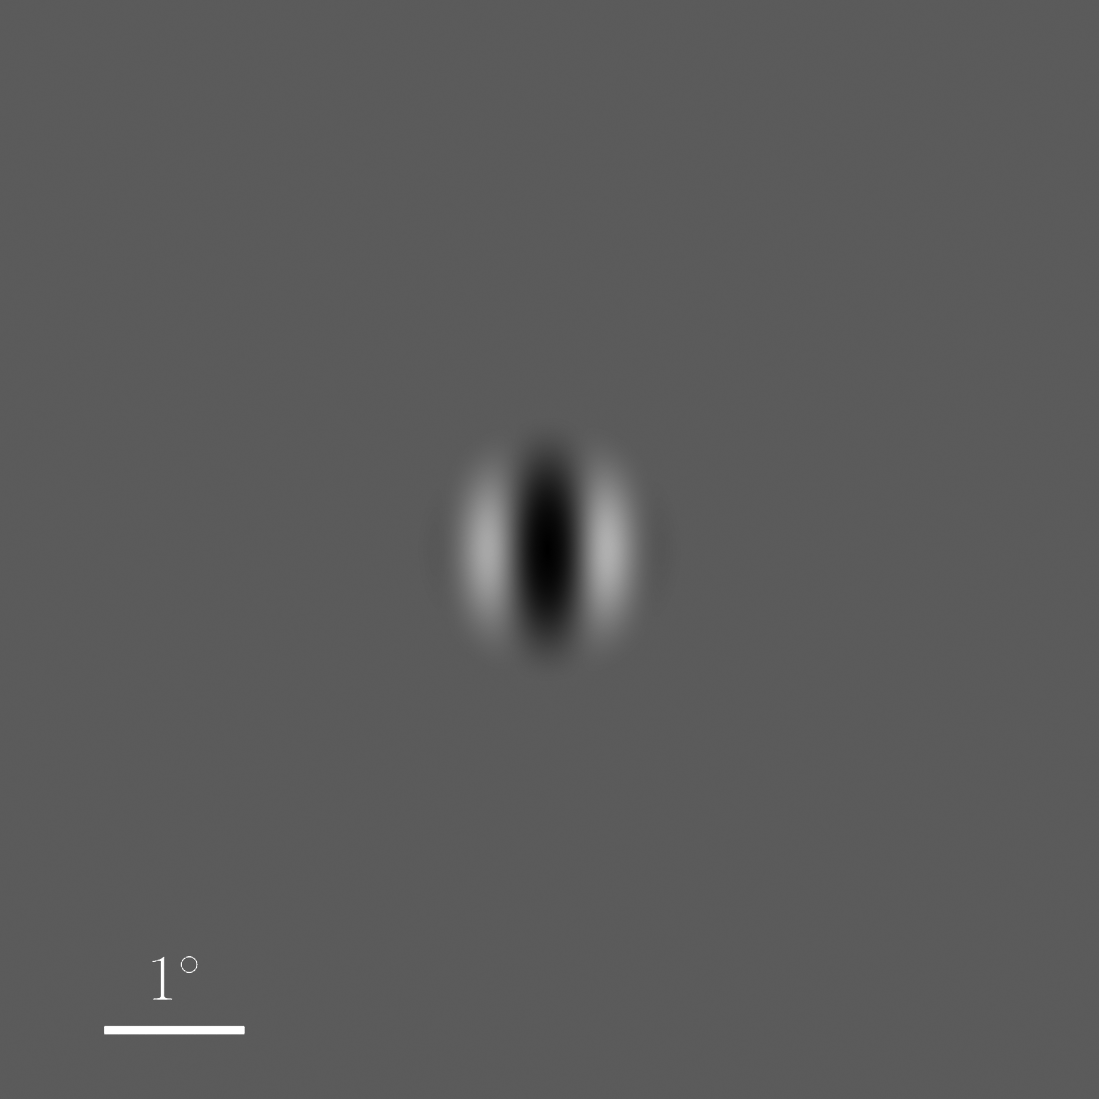
\includegraphics[width=0.48\textwidth]{../jpg/s1_a}}~~
%	\subfloat[Sehwinkel $= 3.6^{\circ}$][Sehwinkel $= 3.6^{\circ}$]{
\includegraphics[width=0.48\textwidth]{../jpg/s2_a}}
%
%	\subfloat[Sehwinkel $= 5.4^{\circ}$][Sehwinkel $= 5.4^{\circ}$]{
\includegraphics[width=0.48\textwidth]{../jpg/s3_a}}~~
%	\subfloat[Sehwinkel $= 7.2^{\circ}$][Sehwinkel $= 7.2^{\circ}$]{
\includegraphics[width=0.48\textwidth]{../jpg/s4_a}}
%
%	\caption[Spatial-Suppression-Bedingungen]{Die vier Mustergrössen $(a - d)$ der \gls{ssauf}.}
%	\label{fig:SpatialSuppression}
%\end{figure}

\subsection{Versuchsablauf \label{subsec:Prozedur}}

Ein Durchgang sah folgendermassen aus: Nach einer Zeitspanne von $440$~ms erschien in der Mitte des Monitors für $560$~ms ein Kreis, der sich über die ersten $200$~ms von einer Grösse von $1.6^{\circ}$ auf eine Grösse von $0.26^{\circ}$ zusammenzog, für $360$~ms diese Grösse beibehielt und anschliessend ausgeblendet wurde. Dieses Vorgehen diente dazu, den Blick der \glspl{vp} in die Bildschirmmitte zu lenken. Nach einem  Intervall von $300$~ms erschien in der Mitte des Monitors ein sich nach links oder rechts bewegendes vertikal schwarz-grau gestreiftes Musters. Die Stelle, an welcher die \glspl{vp} das Muster auf dem Monitor sahen, war stationär. Hinter dieser stationären Stelle bewegte sich das Muster mit einer Geschwindigkeit von $4^\circ / \textnormal{s} $  nach links oder nach rechts. Nach der Darbietungszeit mussten die \glspl{vp} mit einem Tastendruck entscheiden, in welche Richtung sich das Muster bewegt hat. Die \glspl{vp} erhielten die Instruktion, bei einer wahrgenommenen Bewegung nach links mit ihrem linken Zeigefinger die linke Pfeiltaste ($\leftarrow$) und bei einer wahrgenommen Bewegung nach Rechts mit ihrem rechten Zeigefinger die rechte Pfeiltaste ($\rightarrow$) zu drücken. 
Bei einer korrekten Antwort wurde ein Ton abgegeben und die Darbietungszeit des nächsten Musters verringert, bei einer falschen Antwort wurde kein Ton abgegeben und die Darbietungszeit des nächsten Musters erhöht. Die Darbietungszeit des Musters wurde entsprechend dem QUEST-Verfahren \citep{Watson1983} angepasst. Beim QUEST-Verfahren wird mit Hilfe von Grundprinzipien der Bayes-Statistik nach jedem Durchgang eine Schwelle geschätzt. Die Schwellenschätzung wird dann benutzt, um die Darbietungszeit des nächsten Stimulus zu bestimmen. Die \glspl{vp} wurden instruiert, sich bei der Antwortabgabe genügend Zeit zu lassen und möglichst fehlerfrei zu arbeiten. Nach Antwortabgabe startete der nächste Durchgang.

Als Erstes bearbeiteten die \glspl{vp} eine Übungsaufgabe. Dabei wurden die vier Mustergrössen allen \glspl{vp} je drei Mal  in einer pseudorandomisierten Abfolge präsentiert. Die Darbietungszeit aller Mustergrössen betrug zu Beginn der Aufgabe $80$~ms und wurde adaptiv angepasst. Die Übungsaufgabe dauerte etwa eine Minute und wurde nicht ausgewertet. Die $12$~Durchgänge der Übungsaufgabe dienten dazu, dass sich die \glspl{vp} mit der Art der Stimuluspräsentation, der Antworteingabe und dem Ton vertraut machen konnten. 

Als Zweites folgte eine etwas längere Aufgabe. Die \glspl{vp} bearbeiteten drei Wiederholungen, die durch eine Pause von etwa $30$~Sekunden getrennt waren. Eine Wiederholung  bestand aus zwei Schwellenschätzungen pro Mustergrösse. Jede der vier Mustergrössen wurde innerhalb einer Schwellenschätzung sieben Mal präsentiert. Gesamthaft bearbeiteten die \glspl{vp} folglich $3 \times 2 \times 4 \times 7 = 168$ Durchgänge. Die Mustergrössen wurde allen \glspl{vp} in einer pseudorandomisierten Abfolge präsentiert. Die Darbietungszeit der Mustergrössen betrug zu Beginn der Aufgabe $30$~ms und wurde für jede Mustergrösse einzeln über den gesamten Verlauf der $42$~Durchgänge adaptiv angepasst. Die Aufgabe dauerte etwa $7$~Minuten und wurde nicht ausgewertet, weil sich bei einigen \glspl{vp} die Wahrnehmungsleistung während der ersten Durchgänge stark verbessern kann (Duje Tadin, persönliche Mitteilung, 19. August, 2014). Dieser Aufgabenblock diente dazu, diese Trainingseffekte der \glspl{vp} zuzulassen und ihre Leistung auf individuellem Niveau zu festigen. 

Als Drittes bearbeiteten die \glspl{vp} die eigentliche Aufgabe. Die \glspl{vp} bearbeiteten drei Wiederholungen, die durch eine Pause von etwa $1$~Minute getrennt waren. Eine Wiederholung  bestand aus zwei Schwellenschätzungen pro Mustergrösse. Jede der vier Mustergrössen wurde innerhalb einer Schwellenschätzung $22$~Mal präsentiert. Gesamthaft bearbeiteten die \glspl{vp} somit $3 \times 2 \times 4 \times 22 = 528$ Durchgänge. Die Mustergrössen wurde allen \glspl{vp} in einer pseudorandomisierten Abfolge präsentiert. Die Darbietungszeit der Mustergrössen betrug bei Start der Aufgabe $30$~ms und wurde für jede Mustergrösse einzeln über den gesamten Verlauf der $132$~Durchgänge adaptiv angepasst. Daraus resultierten für jede \gls{vp} $\log_{10}$-Schwel\-len\-schätz\-ungen, bei welcher sie in $82\,\%$ der Fälle eine korrekte Antwort abgab respektive die Bewegungsrichtung der Muster richtig erkannt hat.
Die Aufgabe dauerte etwa $25$~Minuten. 

Für jede Mustergrösse wurden die sechs Schwellenschätzungen in eine Rangreihenfolge gebracht, wobei der kleinste und grösste Wert entfernt und die restlichen  vier Schwellenschätzungen gemittelt wurden. Als Basis für alle abhängigen Masse der \gls{ssauf} resultierte so pro \gls{vp} für jede Mustergrösse ($1.8^{\circ}$, $3.6^{\circ}$, $5.4^{\circ}$ und $7.2^{\circ}$) eine $\log_{10}$-Schwellenschätzung.
Der \gls{si} wurde gemäss der Vorgehensweise von \citet{Melnick2013} als Differenz zwischen der $\log_{10}$-Schwellenschätzung für die Mustergrösse $7.2^{\circ}$ und der $\log_{10}$-Schwellenschätzung für die Mustergrösse $1.8^{\circ}$ gebildet. Für die exponentielle Regression wurden die vier~$\log_{10}$-Schwellen\-schätzungen als Exponenten zur Basis~10 verrechnet. Dadurch ergaben sich im Gegensatz zu den $\log_{10}$-Schwellen\-schätzungen leichter interpretierbare Werte im Millisekundenbereich.


\section{Die \glsentrytext{ha}\label{sec:Hick}}

Angelehnt an die Versuchsanordnung von \citet{Rammsayer2007} wurde als Mass für \gls{ms} eine \gls{ha} eingesetzt.

\subsection{Apparatur und Material \label{sub:}}
Präsentiert wurde die Aufgabe auf dem in Abschnitt \ref{sub:ssas} beschriebenen Computer, mit dem einzigen Unterschied, dass die Auflösung des Monitors für die \gls{ha} $1280 \times 1024$ Pixel betrug. Die Antworten der \glspl{vp} wurden mit einer Cedrus RB-830 Tastatur erfasst. 

Die Stimuli wurden mit E-Prime\textsuperscript{\textregistered} \citep{eprime} präsentiert. Die weissen Stimuli wurden auf einem schwarzen Hintergrund präsentiert, welcher eine Leuchtdichte von $2\,\textnormal{cd}/ \textnormal{m}^2$ aufwies. Der horizontale und vertikale Sehwinkel der verwendeten Rechtecke betrug $1.8^{\circ}$ respektive $1.5^{\circ}$. Die Rechtecke wurden auf dem Monitor zentriert dargeboten. Die Stimulianordnung der verwendeten Bedingungen sah folgendermassen aus (siehe Abbildung \ref{fig:Hick}):  In der $0$-Bit-Bedingung wurde ein Rechteck präsentiert. In der $1$-Bit-Bedingung wurden horizontal nebeneinander zwei Rechtecke präsentiert. Die beiden Rechtecke erschlossen zusammen einen horizontalen und vertikalen Sehwinkel von $4.5^{\circ}$ respektive $1.5^{\circ}$. In der $2$-Bit-Bedingung wurden in U-Form vier Rechtecke präsentiert. Die vier Rechtecke erschlossen gemeinsam einen horizontalen und vertikalen Sehwinkel von $7.5^{\circ}$ respektive $4.3^{\circ}$. In der $2.58$-Bit-Bedingung wurden zu den in U-Form angeordneten vier Rechtecken der $2$-Bit-Bedingung in der oberen Reihe je links und rechts ein Rechteck hinzugefügt. Die sechs Rechtecke erschlossen zusammen einen horizontalen und vertikalen Sehwinkel von $12.9^{\circ}$ respektive $4.3^{\circ}$. Der Sehwinkel des imperativen Reizes, einem \enquote{+}, betrug $0.5^{\circ}$ und wurde  immer in der Mitte eines Rechtecks präsentiert. Die Sehwinkel der Stimuli wurden mit einer Kinnstütze, die $61$ cm vom Monitor entfernt war, sichergestellt. Der verwendete Ton wies bei einer Frequenz von $1000$~Hz und einer Lautstärke von $70$~dB eine Länge von $200$~ms auf.

%\begin{figure}[htbp]
%	\centering
%	\subfloat[0-Bit]		[0-Bit-Bedingung]	{
%		\resizebox{.9\textwidth}{!}{
%			\begin{tikzpicture}
%			[scale=1, font=\sffamily, inner sep=0pt, baseline,
%			manifest/.style		= {draw, rectangle, thick, white, inner sep=0pt, minimum width=19mm, minimum height=16mm},
%			invisible/.style	= {draw, rectangle, thick, black!80, inner sep=0pt, minimum width=19mm, minimum height=16mm},
%			visual/.style 		= {draw, rectangle, thick, white, fill=white!100, minimum width= 10.65mm, minimum height=.5mm}]
%			
%			\node [invisible]	at (0,0)							(3)	{};
%			\node [invisible]	[right = 11mm of 3]	  				(4)	{};
%			\node [invisible]	[above left  = 15mm and -3mm of 3]	(2) {};
%			\node [invisible]	[above right = 15mm and -3mm of 4]	(5) {};
%			\node [invisible]	[left  = 11mm of 2]	  				(1)	{};
%			\node [invisible]	[right = 11mm of 5]	  				(6)	{};
%			
%			\node [manifest] at (1.5,1.5)							(9)	{\Huge $+$};
%			
%			\node [visual]		at (-5,-1)	{}							;
%			\node [white]		at (-5,-.6) {\Large$1^{\circ}$}		;
%			
%			\begin{scope}[on background layer]
%				\node [fill=black!80, inner sep= 20pt, fit=(1) (2) (3) (4) (5) (6)] {};
%			\end{scope}
%			\end{tikzpicture}
%}} \newline
%
%\subfloat[1-Bit]		[1-Bit-Bedingung]	{
%	\resizebox{.9\textwidth}{!}{
%		\begin{tikzpicture}
%		[scale=1, font=\sffamily, inner sep=0pt,
%		manifest/.style		= {draw, rectangle, thick, white, inner sep=0pt, minimum width=19mm, minimum height=16mm},
%		invisible/.style	= {draw, rectangle, thick, black!80, inner sep=0pt, minimum width=19mm, minimum height=16mm},
%		visual/.style 		= {draw, rectangle, thick, white, fill=white!100, minimum width= 10.65mm, minimum height=.5mm}]
%		
%		\node [invisible]	at (0,0)							(3)	{};
%		\node [invisible]	[right = 11mm of 3]	  				(4)	{};
%		\node [invisible]	[above left  = 15mm and -3mm of 3]	(2) {};
%		\node [invisible]	[above right = 15mm and -3mm of 4]	(5) {};
%		\node [invisible]	[left  = 11mm of 2]	  				(1)	{};
%		\node [invisible]	[right = 11mm of 5]	  				(6)	{};
%		
%		\node [manifest] at (0,1.5)				(9)		{\Huge $+$}	;
%		\node [manifest] [right = 11mm of 9] 	(10)	{}			;	
%		
%		\node [visual]		at (-5,-1)	{}							;
%		\node [white]		at (-5,-.6) {\Large$1^{\circ}$}		;
%		
%		\begin{scope}[on background layer]
%		\node [fill=black!80, inner sep= 20pt, fit=(1) (2) (3) (4) (5) (6)] {};
%		\end{scope}
%		\end{tikzpicture}
%	}} \newline
%	
%	\subfloat[2-Bit]		[2-Bit-Bedingung]	{
%		\resizebox{.9\textwidth}{!}{
%			\begin{tikzpicture}
%			[scale=1, font=\sffamily, inner sep=0pt,
%			manifest/.style		= {draw, rectangle, thick, white, inner sep=0pt, minimum width=19mm, minimum height=16mm},
%			invisible/.style	= {draw, rectangle, thick, black!80, inner sep=0pt, minimum width=19mm, minimum height=16mm},
%			visual/.style 		= {draw, rectangle, thick, white, fill=white!100, minimum width= 10.65mm, minimum height=.5mm}]
%			
%			\node [invisible]	at (0,0)							(3)	{};
%			\node [invisible]	[right = 11mm of 3]	  				(4)	{};
%			\node [invisible]	[above left  = 15mm and -3mm of 3]	(2) {};
%			\node [invisible]	[above right = 15mm and -3mm of 4]	(5) {};
%			\node [invisible]	[left  = 11mm of 2]	  				(1)	{};
%			\node [invisible]	[right = 11mm of 5]	  				(6)	{};
%			
%			\node [manifest]	at (0,0)							(3)	{};
%			\node [manifest]	[right = 11mm of 3]	  				(4)	{};
%			\node [manifest]	[above left  = 15mm and -3mm of 3]	(2) {\Huge $+$};
%			\node [manifest]	[above right = 15mm and -3mm of 4]	(5) {};	
%			
%			\node [visual]		at (-5,-1)	{}							;
%			\node [white]		at (-5,-.6) {\Large$1^{\circ}$}		;
%			
%			\begin{scope}[on background layer]
%			\node [fill=black!80, inner sep= 20pt, fit=(1) (2) (3) (4) (5) (6)] {};
%			\end{scope}
%			\end{tikzpicture}
%		}} \newline
%		
%		\subfloat[$2.58$-Bit]		[$2.58$-Bit-Bedingung]	{
%			\resizebox{.9\textwidth}{!}{
%				\begin{tikzpicture}
%				[scale=1, font=\sffamily, inner sep=0pt,
%				manifest/.style		= {draw, rectangle, thick, white, inner sep=0pt, minimum width=19mm, minimum height=16mm},
%				invisible/.style	= {draw, rectangle, thick, black!80, inner sep=0pt, minimum width=19mm, minimum height=16mm},
%				visual/.style 		= {draw, rectangle, thick, white, fill=white!100, minimum width= 10.65mm, minimum height=.5mm}]
%				
%				\node [invisible]	at (0,0)							(3)	{};
%				\node [invisible]	[right = 11mm of 3]	  				(4)	{};
%				\node [invisible]	[above left  = 15mm and -3mm of 3]	(2) {};
%				\node [invisible]	[above right = 15mm and -3mm of 4]	(5) {};
%				\node [invisible]	[left  = 11mm of 2]	  				(1)	{};
%				\node [invisible]	[right = 11mm of 5]	  				(6)	{};
%				
%				\node [manifest]	at (0,0)							(3)	{};
%				\node [manifest]	[right = 11mm of 3]	  				(4)	{};
%				\node [manifest]	[above left  = 15mm and -3mm of 3]	(2) {};
%				\node [manifest]	[above right = 15mm and -3mm of 4]	(5) {};
%				\node [manifest]	[left  = 11mm of 2]	  				(1)	{};
%				\node [manifest]	[right = 11mm of 5]	  				(6)	{\Huge $+$};
%				
%				\node [visual]		at (-5,-1)	{}							;
%				\node [white]		at (-5,-.6) {\Large$1^{\circ}$}		;
%				
%				\begin{scope}[on background layer]
%				\node [fill=black!80, inner sep= 20pt, fit=(1) (2) (3) (4) (5) (6)] {};
%				\end{scope}
%				\end{tikzpicture}
%			}} \newline
%			
%			\caption[Hick Bedingungen]{Die vier Bedingungen $(a - d)$ der \gls{ha}. }
%			\label{fig:Hick}
%\end{figure}




\subsection{Versuchsablauf \label{subsec:HVersuchsablauf}}


In der $0$-Bit-Bedingung bearbeiteten die \glspl{vp} $32$ Durchgänge. Jeder Durchgang startete nach $1100$ ms mit der Präsentation eines Rechtecks. Nach einer variablen Zeitdauer, \gls{soa} genannt, welche $1000$, $1333$, $1666$ oder $2000$ ms betrug, wurde der imperative Reiz, ein \enquote{+}, eingeblendet. Die \glspl{vp} wurden angewiesen, mit dem Zeigefinger ihrer dominanten Hand so rasch als möglich auf die vorgesehene Antworttaste zu drücken. Bei einer Antwortabgabe nach Einblenden des imperativen Reizes folgte ein Ton. Bei einer Antwortabgabe vor Einblenden des imperativen Reizes folgte kein Ton. In beiden Fällen führte eine Antwortabgabe zur Ausblendung der Stimuli und zum Start des nächsten Durchganges.

Die $1$-Bit-Bedingung unterschied sich von der $0$-Bit-Bedingung in der Anzahl dargebotener Rechtecke und der Tonabgabe. Der imperative Reiz trat im linken oder im rechten Rechteck auf. Die \glspl{vp} erhielten die Anweisung, beim Auftreten des imperativen Reizes im linken Rechteck mit ihrem linken Zeigefinger und beim Auftreten des imperativen Reizes im rechten Rechteck mit ihrem rechten Zeigefinger so rasch als möglich auf die dem jeweiligen Finger zugewiesene Antworttaste zu drücken. Bei einer korrekten Antwortabgabe nach Einblendung des imperativen Reizes folgte ein Ton. Bei einer Antwortabgabe vor Einblendung des imperativen Reizes oder bei einer falschen Antwortabgabe folgte kein Ton.

Die $2$-Bit-Bedingung unterschied sich von der $1$-Bit-Bedingung lediglich in der Anzahl präsentierter Rechtecke. Der imperative Reiz trat entweder im oberen linken, unteren linken, oberen rechten oder unteren rechten Rechteck auf. Die \glspl{vp} wurden angewiesen, beim Auftreten des imperativen Reizes im oberen linken Rechteck mit ihrem linken Mittelfinger, beim Auftreten des imperativen Reizes im unteren linken Rechteck mit ihrem linken Zeigefinger,  beim Auftreten des imperativen Reizes im oberen rechten Rechteck mit ihrem rechten Mittelfinger und beim Auftreten des imperativen Reizes im unteren rechten Rechteck mit ihrem rechten Zeigefinger so rasch als möglich auf die dem jeweiligen Finger zugewiesene Antworttaste zu drücken.

Die $2.58$-Bit-Bedingung unterschied sich von der $2$-Bit-Bedingung nur in der Anzahl präsentierter Rechtecke. Der imperative Reiz trat entweder im oberen äusseren linken, oberen inneren linken, unteren linken, oberen äusseren rechten, oberen inneren rechten oder unteren rechten Rechteck auf. Die \glspl{vp} wurden angewiesen, beim Auftreten des imperativen Reizes im oberen äusseren linken Rechteck mit ihrem linken Ringfinger, beim Auftreten des imperativen Reizes im oberen inneren linken Rechteck mit ihrem linken Mittelfinger, beim Auftreten des imperativen Reizes im unteren linken Rechteck mit ihrem linken Zeigefinger, beim Auftreten des imperativen Reizes im oberen äusseren Rechteck mit ihrem rechten Ringfinger, beim Auftreten des imperativen Reizes oberen inneren rechten Rechteck mit ihrem rechten Mittelfinger und beim Auftreten des imperativen Reizes im unteren rechten Rechteck mit ihrem rechten Zeigefinger so rasch als möglich auf die dem jeweiligen Finger zugewiesene Antworttaste zu drücken.

Die Bedingungen wurden von allen \glspl{vp} in aufsteigender Reihenfolge ($0$-, $1$-, $2$-, $2.58$-Bit-Bedingung) bearbeitet. Jeder Bedingung gingen acht  Übungsdurchgänge voraus, damit sich die \glspl{vp} mit der Art der Stimuluspräsentation, der Antworteingabe und dem Ton vertraut machen konnten. 
Der imperative Reiz trat in der $1$-, $2$- und $2.58$-Bit-Bedingung für alle \glspl{vp} in einer pseudorandomisierten Abfolge mit der identischen, ausbalancierten \gls{soa} am identischen, über die $32$~Durchgänge der Bedingungen ausbalancierten Ort auf. Insgesamt dauerte die Aufgabe etwa $15$~Minuten. 

Pro Bedingung wurde für jede \gls{vp} der Mittelwert und die Standardabweichung aller korrekten Antworten bestimmt, die zwischen $100$ und $2500$~ms lagen. Basierend auf diesen Berechnungen wurden für jede \gls{vp} in jeder Bedingung diejenigen Durchgänge entfernt, welche eine \gls{rz} $\geq$ \gls{m} $+\,3\,\times$ \gls{sd} aufwiesen. Nach dieser intraindividuellen Ausreisserkontrolle wurden die verbliebenen Durchgänge innerhalb einer Bedingung gemittelt und für jede \gls{vp} als Leistungsmass der Bedingung der \gls{ha} verwendet.


\section{Erfassung der psychometrischen Intelligenz \label{sec:Intelligenz}}

\glsunset{bist} % see http://tex.stackexchange.com/questions/30167/suppress-the-glossary-expansion-at-first-occurance


Psychometrische Intelligenz wurde mit einer modifizierten Kurzversion des \acrlong{bist} \citep[\gls{bist};][]{Jaeger1997} erfasst. Die fähigkeitstheoretische Grundlage des Tests ist das integrativ konzipierte bimodale und hierarchische \gls{bism} von \citet[][siehe Abbildung \ref{fig:BIS}]{Jaeger1984}. 
\begin{figure}[htb]
	\centering
	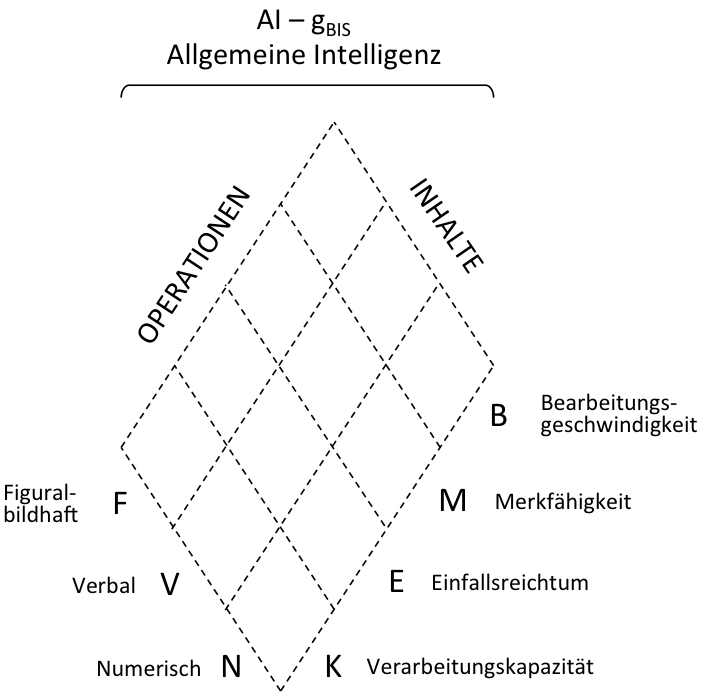
\includegraphics[width=0.8\textwidth]{../jpg/BIS}
	\caption[Das BIS]{Das BIS von \citet{Jaeger1984}.}
	\label{fig:BIS}
\end{figure} 

Als integratives Modell ist das \gls{bism} zu bezeichnen, weil \citet{Jaeger1984} bei der Konstruktion des Modells versucht hat, die Vielfalt intellektueller Leistungsformen möglichst umfassend zu repräsentieren.
Bimodal ist das \gls{bism}, weil das Modell zwei Modalitäten aufweist, unter welchen Leistungen und Fähigkeiten klassifiziert werden können. 
Das \gls{bism} trennt dabei zwischen sogenannten Operationen und Inhalten. Innerhalb der Modalität Operationen werden die vier Fähigkeitsbündel Verarbeitungskapazität, Bearbeitungsgeschwindigkeit, Merkfähigkeit und Einfallsreichtum unterschieden. 
\gls{k} steht für die Fähigkeit, komplexe Informationen von Aufgaben zu verarbeiten, die nicht auf Anhieb zu lösen sind, sondern die erst durch vielfältiges Beziehungsstiften, formallogisch exaktes Denken und sachgerechtes Beurteilen von Informationen zu lösen sind. 
\gls{b} beschreibt das Arbeitstempo, die Auffassungsleichtigkeit und die Konzentrationskraft beim Lösen von einfach strukturierten Aufgaben mit geringem Schwierigkeitsgrad. 
\gls{M} spiegelt die Fähigkeit wider, sich etwas aktiv einzuprägen, etwas kurzfristig wieder zu erkennen oder zu reproduzieren. 
\gls{e} beschreibt die Fähigkeit, flexible Ideen zu produzieren und über vielfältige Vorstellungen von Problemen zu verfügen. 
Innerhalb der Modalität Inhalte lässt sich nach \citet{Jaeger1984} sprachgebundenes Denken von zahlengebundenem Denken und anschauungsgebundenem, figural-bildhaftem Denken unterscheiden.
\Gls{v} beschreibt den Grad der Aneignung und der Verfügbarkeit des Beziehungssystems Sprache.
\Gls{n} steht für das Ausmass der Aneignung und der Verfügbarkeit des Beziehungssystems Zahlen.
\Gls{f} spiegelt die Fähigkeit wider, Aufgabenmaterial zu verarbeiten, welches bildhaftes beziehungsweise räumliches Vorstellen erfordert.

Auf höchster Hierarchiestufe des \gls{bism} steht als Integral aller sieben Fähigkeiten (\gls{k}, \gls{b}, \gls{M}, \gls{e}, \gls{v}, \gls{n} und \gls{f}) die \gls{ai}. Die \gls{ai} und die Fähigkeiten unterscheiden sich aber lediglich im Differenzierungsgrad. \gls{ai} bildet Intelligenzleistungen gemäss \citet{Jaeger1984} aus grosser Distanz ab, während die sieben Fähigkeiten auf der Ebene darunter Intelligenzleistungen aus geringerer Distanz mit feinerem Auflösungsgrad abbilden. Untersuchungen zum \gls{bism} konnten die postulierte Struktur des \gls{bist} replizieren  und Zusammenhänge mit anderen Intelligenzmodellen wie denjenigen von \citet{Cattell1971}  oder von \citet{Carroll1993} herstellen \citep{Bucik1996, Beauducel2002, Suess2002}.

Die von \citet{Jaeger1997} vorgeschlagene Kurzversion des \gls{bist} enthält $15$ Subtests. Die Operationen \gls{b}, \gls{M} und \gls{e} werden darin mit je einem Subtest pro Inhalt erfasst, wobei \gls{k} mit zwei Subtests pro Inhalt erfasst wird. Bei der Modellierung der Daten mittels Strukturgleichungsmodellen hätte dies bei der vorliegenden Arbeit zu einer Überrepräsentation von \gls{k} im \gls{gfaktor} geführt. Um dies zu vermeiden, wurden die Operationen \gls{b} und \gls{M} um je einen Subtest pro Inhalt angereichert. Grundlage für die Auswahl der Subtests bildeten die Erkenntnisse von \citet{Wicki2014}, wobei bei der Entscheidung über die Aufnahme der Subtests ökonomische (Bearbeitungszeit der Subtests) und teststatistische (Trennschärfe und Reliabilität der Subtests)  Gesichtspunkte berücksichtigt wurden. Die Kurzversion von \citet{Jaeger1997} wurde mit folgenden Subtests ergänzt: Klassifizieren von Wörtern, Old English, Rechen-Zeichen, Wege-Erinnern, Worte Merken und Zweistellige Zahlen. 
\citet{Wicki2014} berichtet für diese modifizierte Kurzversion für die Operationen \gls{k}, \gls{b} und \gls{M} interne Konsistenzen von Cronbachs $\alpha=.61-.73$ und Konstruktreliabilitäten, gemessen mit \citeauthor{McDonald1999}'s \citeyearpar{McDonald1999} Omegakoeffizienten, von $\Omega = .58-.64$.
Auf Subtests der Operation \gls{e} wurde gänzlich verzichtet, weil zum einen unklar ist, wie Einfallsreichtum und Intelligenz zusammenhängen \citep{Kim2005} und zum anderen weil \citet{Jaeger1997} unbefriedigende Objektivitätswerte berichten. 
Alle eingesetzten Subtests, deren Beschreibung sowie Zuordnung zu den jeweiligen Operationen und Inhalte sind Tabelle \ref{tab:BIS} zu entnehmen.
\begin{sidewaystable}
	
	
	\begin{adjustbox}{width=\textwidth,totalheight=.9\textheight,keepaspectratio}
		
		\begin{threeparttable}
			\captionsetup{labelsep = none}
			\caption[Die Subtests des BIS-Test]{\newline  \textit{Reihenfolge der eingesetzten Subtests des BIS-Test} \vspace{.2cm}}
			\label{tab:BIS}
			
			\begin{tabular}{l l c c c c p{.0001cm} c c c p{20cm}}
				
				\hline
				Nr.	&	Name	&	Abkürzung	& \multicolumn{3}{c}{Operation}	&	&	\multicolumn{3}{c}{Inhalt}	&	Beschreibung\\
				\cline{4-6}
				\cline{8-10}
				&&&	K	& B & M	&&	V	&	N	&	F	& \\
				\hline
				1				&	Unvollständige Wörter*	&	UW			&&	\checkmark	&&&\checkmark&&& In vorgegebenen Wörtern fehlen einige Buchstaben, welche zu ergänzen sind (z.B. F\_scher)	\\
				2				&	Orientierungs-Gedächtnis	&	OG		&&&	\checkmark	&&&&\checkmark& Auf einem Stadtplanausschnitt markierte Gebäude müssen eingeprägt und unmittelbar danach wiedergegeben werden\\
				3				&	Zahlenreihen			&	ZN			&	\checkmark	&&&&&\checkmark&& Nach bestimmten Regeln aufgebaute Zahlenreihen sind um ein weiteres Glied zu ergänzen (z.B. 2 5 8 11 14 17 ?)\\
				4				&	Analogien				&	AN			&	\checkmark	&&&&&&\checkmark& Analogien mit Form $A:B=C:\,?$ müssen ergänzt werden, wobei die Analogien aus geometrischen Formen bestehen\\
				5				&	X-Grösser				&	XG			&&	\checkmark	&&&&\checkmark&& Zahlen, die um $3$ grösser sind als die unmittelbar vorangegangene Zahl müssen so schnell wie möglich durchgestrichen werden (z.B. 18 20 24 \cancel{27} 13 18 \cancel{21} \ldots)\\
				6				&	Wortanalogien			&	WA			&	\checkmark	&&&&\checkmark&&& Wortanalogien der Form \enquote{Huhn zu Küken} wie \enquote{Kuh zu ?} müssen vervollständigt werden\\
				7				&	Zahlenpaare				&	ZP			&&&	\checkmark	&&&\checkmark&& Zahlenpaare der Form 71 -- 918 sind einzuprägen. Das jeweils zweite Glied ist anschliessend unter vier Distraktoren zu identifizieren\\
				8				&	Tatsache-Meinung		&	TM			&	\checkmark	&&&&\checkmark&&& Sätze müssen daraufhin geprüft werden, ob sie eher eine Tatsache oder eher eine Meinung wiedergeben\\
				9				&	Buchstaben-Durchstreichen&	BD			&&	\checkmark	&&&&&\checkmark& Alle \enquote{x} müssen in Zeilen von Buchstaben durchgestrichen werden (z.B. sys\cancel{x}kdihj\cancel{x}\ldots)\\
				10				&	Schätzen				&	SC			&	\checkmark	&&&&&\checkmark&& Rechenaufgaben der Form $118492-3684-2106-4768=\,?$ müssen durch einfache rechnerische Überlegungen geschätzt bzw. gelöst werden\\
				11				&	Sinnvoller Text			&	ST			&&&	\checkmark	&&\checkmark&&& Verbale Detailangaben in einem Text sind einzuprägen und unmittelbar danach zu reproduzieren\\
				12				&	Charkow					&	CH			&	\checkmark	&&&&&&\checkmark& Eine Folge von Strichzeichnungen, die nach einer bestimmten Regel aufgebaut ist, ist um die beiden folgenden Glieder zu ergänzen\\
				13				&	Teil-Ganzes				&	TG			&&	\checkmark	&&&\checkmark&&& In Wortlisten sind zwei aufeinander folgende Wörter, die in der Beziehung Ganzes/zugehöriger Teil zueinander stehen zu markieren (z.B. Baum, \cancel{Blatt}, Stein, Haus, \cancel{Dach}, \ldots)\\
				14				&	Rechen--Zeichen			&	RZ			&&	\checkmark	&&&&\checkmark&& In  einfachen vorgegebenen Gleichungen stehen anstelle von Plus- oder Minuszeichen leere Kästchen. Die richtigen Rechenzeichen sind einzutragen\\
				15				&	Worte merken			&	WM			&&&	\checkmark	&&\checkmark&&& Eine Liste von Wörtern ist einzuprägen und unmittelbar danach in beliebiger Reihenfolge zu reproduzieren\\ 
				16				&	Klassifizieren von Wörtern&	KW			&&	\checkmark	&&&\checkmark&&& In Spalten von Wörtern sind alle Worte, die Pflanzen bezeichnen, durchzustreichen\\
				17				&	Zweistellige Zahlen		&	ZZ			&&&	\checkmark	&&&\checkmark&& Eine Reihe zweistelliger Zahlen ist einzuprägen und unmittelbar danach in beliebiger Reihenfolge zu reproduzieren\\
				18				&	Old English				&	OE			&&	\checkmark	&&&&&\checkmark& In Buchstabenreihen sind alle in einem vorgegebenen Schrifttyp gedruckten Buchstaben durchzustreichen\\
				19				&	Wege--Erinnern			&	WE			&&&	\checkmark	&&&&\checkmark& Ein in einem Stadtplanausschnitt eingezeichneter Weg ist einzuprägen und unmittelbar danach zu reproduzieren\\
				
				\hline

			\end{tabular}
			
			\begin{tablenotes}[flushleft]
				\footnotesize				% font size
				\setlength\labelsep{0pt}	% no indent on second line
				\item \textit{Anmerkungen.} * Der Subtest UW wurde als Aufwärmaufgabe verwendet und floss nicht in die Auswertung mit ein. K~=~Verarbeitungskapazität, B~=~Bearbeitungsgeschwindigkeit, M~=~Merkfähigkeit, V~=~verbal, N~=~numerisch, F~=~figural--bildhaft.
			\end{tablenotes}
		\end{threeparttable}
	\end{adjustbox}
\end{sidewaystable}

Die $19$ Subtests wurden den \glspl{vp} nach der in Tabelle \ref{tab:BIS} aufgeführten Reihenfolge vorgelegt und gemäss dem Manual des \gls{bist} instruiert. 
Die Bearbeitung der Subtests dauerte insgesamt $50$ Minuten.
Die Aufwärmaufgabe \gls{uw} wurde nicht ausgewertet. Die Rohwerte der restlichen $18$~Subtests wurden \textit{z}-standardisiert. 
Für die Beantwortung der Fragestellungen 1 und 2 wurden alle $18$~\textit{z}-stand\-ard\-isier\-ten Subtests gemittelt. Dadurch resultierte für jede \glspl{vp} ein \textit{z}-standardisiertes Mittel ihrer Leistung. 
Um für die Beantwortung der Fragestellungen 3, 4 und 5 einen \gls{gfaktor} zu bilden, wurden die $18$~\textit{z}-standardisierten Subtests innerhalb ihrer zugehörigen Operation gemittelt. Damit flossen in jede Operation (\gls{k}, \gls{b} und \gls{M}) zwei Subtests aus dem Bereich \gls{v}, zwei Subtests aus dem Bereich \gls{n} und zwei Subtests aus dem Bereich \gls{f} (insgesamt sechs Subtests) ein. Der \gls{gfaktor} wurde anschliessend aus den drei gemittelten \textit{z}-Werten der Operationen \gls{k}, \gls{b} und \gls{M} abgeleitet.


\section{Weitere Instrumente}

Im Rahmen der Untersuchung wurden den \glspl{vp} Fragebögen und weitere Com\-put\-er-Auf\-gaben zur Bearbeitung vorgelegt. Sie sind für die Fragestellungen dieser Arbeit nicht relevant und werden deshalb im folgenden Abschnitt nur kurz beschrieben.


\subsection{Fragebögen}

\subsubsection*{Persönliche Angaben}
Die Erfassung persönlicher Angaben fand in zwei Teilen statt. In einem ersten Teil machten die \glspl{vp} schriftlich Angaben zu ihrer Muttersprache, Seh- und Hörfähigkeit, ihren chronischen Krankheiten und ihrem Medikamenten- sowie Nikotinkonsum. In einem zweiten Teil machten sie computergestützt Angaben zu ihrem Alter, Geschlecht, Bildungsniveau, Koffeinkonsum,  Videospielhäufigkeit, Musikinstrumenterfahrung und Vertrautheit mit dem Zehnfingersystem beim Computerschreiben.


\subsubsection*{Kurzform der deutschen Übersetzung des revidierten \gls{epq-rk}}
Die \glspl{vp} haben  computergestützt die Kurzform der deutschen Übersetzung des \gls{epq-rk} von \citet{Ruch1999} bearbeitet. Der Fragebogen enthält insgesamt $50$~Fragen, darunter $14$~Items zur Erfassung von Psychotizismus, $12$~Items zur Erfassung von Extraversion, $12$~Items zur Erfassung von Neurotizismus und $12$~Items zur Erfassung der individuellen Neigung, sozial erwünschte Antworten abzugben.

\subsubsection*{Deutsche Übersetzung des \gls{dii}}
Die deutsche Übersetzung des \gls{dii} stammt von \citet{Kuhmann1996} und beinhaltet insgesamt $23$~Items, darunter $11$~Items zur Erfassung der funktionalen Impulsivität und  $12$~Items zur Erfassung der dysfunktionalen Impulsivität. Der Fragebogen wurde von den \glspl{vp} computergestützt bearbeitet.

\subsection{Zeitverarbeitungsaufgaben}


\subsubsection*{Zeitdauerdiskrimination im Millisekundenbereich mit gefüllten und leeren Intervallen}

Die \glspl{vp} bekamen über Lautsprecher hintereinander eine Standardtondauer und eine variable Vergleichstondauer dargeboten. Danach mussten die \glspl{vp} jeweils mit einem Tastendruck entscheiden, ob die erste oder die zweite Tondauer länger war. Bei einer korrekten Antwort verringerte sich die Differenz zwischen der Standard- und der Vergleichstondauer und bei einer falschen Antwort erhöhte sich diese Differenz. Die Aufgabe wurde einmal mit gefüllten Zeitintervallen (das heisst mit jeweils zwei kontinuierlichen Tönen) und einmal mit leeren Zeitintervallen (das heisst die Töne waren durch einen Klick am Anfang und einen Klick am Schluss des Intervalls gekennzeichnet) durchgeführt. Diese Aufgaben dauerte insgesamt etwa $15$ Minuten. Der Aufgabenaufbau war vergleichbar mit demjenigen von \citet{Stauffer2011}. 


\subsubsection*{Zeitgeneralisation im Millisekundenbereich}

Die Aufgabe der \glspl{vp} war es, in einer Lernphase die über Lautsprecher fünf Mal präsentierte Standardtonlänge einzuprägen. Danach folgte die eigentliche Aufgabe: Es wurden in zufälliger Reihenfolge die Standardtonlänge und sechs Vergleichstonlängen präsentiert. Die \glspl{vp} mussten nach jeder Tonlänge mit einem Tastendruck entscheiden, ob die präsentierte Tonlänge von gleicher Länge war wie die Standardtonlänge oder nicht. Diese Aufgabe dauerte insgesamt etwa $5$ Minuten \citep[siehe][]{Stauffer2011}.

\subsubsection*{Rhythmuswahrnehmung}

Die \glspl{vp} hatten die Aufgabe, sechs über Lautsprecher in unregelmässigen Abständen präsentierte Töne von jeweils $3$~ms Dauer auf rhythmische Darbietung hin zu beurteilen. 
Gaben die \glspl{vp} an, den Rhythmus als regelmässig wahrgenommen zu haben, wurde die Abweichung des Interstimulusintervalls beim nächsten Durchgang erhöht. Gaben die \glspl{vp} an, den Rhythmus als unregelmässig wahrgenommen zu haben, wurde die Abweichung des Interstimulusintervalls beim nächsten Durchgang verringert.
Die Aufgabe dauerte insgesamt etwa $5$ Minuten \citep[siehe][]{Stauffer2011}.

\subsection{\gls{ita}}

Die auf einem Computermonitor präsentierten Stimuli der \gls{ita} \citep{Vickers1972} bestanden aus zwei ungleich langen vertikalen Linien, die an ihren oberen Enden mit einer horizontalen Linie verbunden waren. Bei jedem Durchgang wurde die kürzere vertikale Linie zufällig links oder rechts präsentiert und nach der Darbietungszeit mit einer Pi-förmigen Abbildung, die gleich lange vertikale Linien aufwies, maskiert. Die Aufgabe der \glspl{vp} bestand darin anzugeben, ob die linke oder die rechte vertikale Linie länger war. Eine korrekte Antwort verringerte und eine falsche Antwort erhöhte die Darbietungszeit des nächsten Stimulus. Die Aufgabe dauerte insgesamt etwa $5$ Minuten.


\section{Untersuchungsablauf \label{sec:Versuchsablauf}}

Die Untersuchung wurde vor Datenerhebungsbeginn von der Ethikkomission der philosophisch-humanwissenschaftlichen Fakultät der Universität Bern gutgeheissen. Die \glspl{vp} nahmen an zwei Sitzungen teil, welche $2$ bis $14$~Tage voneinander getrennt waren. Zwei \glspl{vp} hatten krankheitsbedingt ein längeres Intervall zwischen den beiden Sitzungen ($18$ und $30$ Tage).

\subsection{Sitzung 1}

Die \glspl{vp} wurden in Gruppen von zwei bis sechs Personen in einem $18\,\textnormal{m}^2$ grossen Raum an Einzeltische gesetzt. Die Tische waren so weit voneinander entfernt, dass die \glspl{vp} nicht durch den Nachbarn gestört werden oder abschreiben konnten. 
Ohne die Fragestellungen der Arbeit zu offenbaren, klärte der Versuchsleiter\footnote{In dieser Arbeit wird der Einfachheit halber nur die männliche Form verwendet. Die weibliche Form ist selbstverständlich immer mit eingeschlossen.} die \glspl{vp} über den Zweck der Untersuchung auf, informierte sie über den Ablauf der bevorstehenden Sitzung und nahm die Einverständniserklärungen der \glspl{vp} entgegen. Danach wurden der Reihenfolge nach folgende Daten erhoben und Instrumente eingesetzt:

\begin{enumerate}
	\item Persönliche Angaben Teil 1
	\item \acrshort{bist}
	\item Persönliche Angaben Teil 2
	\item \gls{epq-rk}
	\item \gls{dii}
\end{enumerate}

\noindent Diese erste Sitzung dauerte insgesamt etwa 90 Minuten.

\subsection{Sitzung 2}
Die zweite Sitzung fand als Einzeltestung in einer $5\,\textnormal{m}^2$ grossen, schallgedämpften Kabine statt. 
Der Versuchsleiter informierte die \glspl{vp} über den Ablauf der bevorstehenden Sitzung und legte ihnen am Computer der Reihenfolge nach folgende Aufgaben vor:

\begin{enumerate}
	\item	\gls{ssauf}
	\item	Die fünf Aufgaben
			\begin{dinglist}{43}
				\item \gls{ha}
				\item Zeitdauerdiskrimination im Millisekundenbereich mit gefüllten Intervallen
				\item Zeitdauerdiskrimination im Millisekundenbereich mit leeren Intervallen
				\item Zeitgeneralisation im Millisekundenbereich
				\item Rhythmuswahrnehmung
			\end{dinglist}
			wurden über alle \glspl{vp} hinweg vollständig permutiert, was in $5\,! = 120$ unterschiedlichen Reihenfolgen resultierte. Nach $120$~\glspl{vp} wurden die Reihenfolgen wiederholt, das heisst  \gls{vp} $121$ bearbeitete die Aufgaben in der gleichen Reihenfolge wie \gls{vp} 1, \gls{vp} $122$ bearbeitete die Aufgaben in der gleichen Reihenfolge wie \gls{vp} 2 und so weiter.
	\item	\gls{ita}
\end{enumerate}

Nach der letzten Aufgabe wurden die \glspl{vp} vollständig über das Ziel der Untersuchung aufgeklärt und entlöhnt. Diese zweite Sitzung dauerte inklusive einer fünfminütigen Pause nach 50 Minuten insgesamt etwa 120 Minuten.



%\clearpage
\section{Statistische Analyse \label{sec:StatistischeAnalyse}}

Alle Berechnungen wurden in R \citep{R} durchgeführt, dessen Basisfunktionen mit folgenden Paketen ergänzt wurde:
{coin} \citep{coin},
dplyr \citep{dplyr},
effsize \citep{effsize},
ez \citep{ez},
lavaan \citep{lavaan},
Metrics \citep{Metrics},
multcomp \citep{multcomp},
nlme \citep{nlme},
nlstools \citep{nlstools},
nortest \citep{nortest},
pbapply \citep{pbapply},
plotrix \citep{plotrix},
ppcor \citep{ppcor},
psych \citep{psych},
readxl \citep{readxl},
reshape2 \citep{reshape2},
rprime \citep{rprime},
R.matlab \citep{R.matlab} und
semPlot \citep{semPlot} .
Als Editor diente RStudio \citep{RStudio}.

Die Fragestellungen 3, 4 und 5 (siehe Seite \pageref{text:Fragestellung3}) werden mittels \gls{kfa} beantwortet. Die Güte einer \gls{kfa} kann anhand einer Vielzahl von unterschiedlichen Kennwerten beurteilt werden, weshalb hier die für diese Arbeit wichtigen Kennwerte kurz vorgestellt werden.








\subsubsection*{\gls{cst}}

KURZ NOCHMALS SAGEN, WAS GUTER CHI-QUADRAT WERT IST!

Der \gls{cst} ist ein Modelltest, der angibt, wie stark sich die empirische Var\-ianz-Ko\-var\-ianz\-ma\-trix von der theoretischen, vom Modell implizierten Var\-ianz-Ko\-var\-ianz\-ma\-trix unterscheidet \citep{Kline2011}. Die dafür berechnete Teststatistik folgt in grossen Stichproben und unter der Voraussetzung der multivariaten Normalverteilung einer zentralen Chi Quad\-rat-Ver\-teil\-ung und wird deshalb auch als $\upchi^2_{m}$ bezeichnet. Die Freiheitsgrade für den $\upchi^2$-Test ergeben sich aus den Freiheitsgraden des zu testenden Modells ($df_{m}$). Wenn $\upchi^2_{m}=0$ ist, stimmt die empirische Var\-ianz-Ko\-var\-ianz\-ma\-trix mit der vom Modell implizierten Varianz-Kovarianzmatrix ohne Abweichung überein und die empirischen Daten passen perfekt zum theoretischen Modell. Bildet das Modell die Daten nicht gut ab, wird $\upchi^2_{m}>0$. Liegt $\upchi^2_{m}$ über dem kritischen $\upchi^2_{df}$, sind die Abweichungen zwischen der empirischen und der theoretischen Varianz-Kovarianzmatrix grösser als durch den Stichprobenfehler erwartet, und die Nullhypothese wird verworfen. Wenn ein korrekt spezifiziertes Modell mit mehreren Zufallsstichproben geprüft wird, liegt der Erwartungswert von $\upchi^2_{m}$ bei $df_{m}$, und $\upchi^2_{m}$ würde bei einem $\alpha$-Fehler von $5\,\%$ bei 19 von 20 Stichproben im nicht-signifikanten Bereich liegen.


\subsubsection*{\gls{cfi}}
Der \gls{cfi} lässt sich der Klasse der inkrementellen Fit Indizes zuordnen und wurde von \citet{Bentler1990} entworfen. Die Formel lautet

$$ \textnormal{CFI} = 1 - \frac{\upchi^2_{m}-df_{m}}{\upchi^2_{b}-df_{b}} $$

\noindent Im Zähler wird $df_{m}$ von $\upchi^2_{m}$ subtrahiert. Im Nenner des Bruchs wird die gleiche Differenz mit den Werten des Baseline Modells ($df_{b}$ und $\upchi^2_{b}$) gebildet.
Das Baseline Modell nimmt keinerlei Zusammenhänge zwischen den manifesten Variablen an und wird deshalb auch als \enquote{independence model} bezeichnet. Zieht man den beschriebenen Quotienten von Eins ab, ergibt sich ein Mass für die relative Verbesserung des angenommenen Modells gegenüber dem Baseline Modell. Aus der Formel folgt, dass \gls{cfi} $= 1$ ergibt, wenn $\upchi^2_{m} \leq df_{m}$ ist. Das bedeutet aber auch, dass ein \gls{cfi} von Eins nicht mit einem perfekten Fit ($\upchi^2_{m} = 0$) gleichzusetzen ist. Ein \gls{cfi} von $.95$ ist laut \citet{Hu1999} als guter Fit zu bezeichnen.

\subsubsection*{\gls{rmsea}}
Die Anzahl Freiheitsgrade eines Modells geben an, auf wie vielen Dimensionen die empirischen Daten vom Modell abweichen können. Der RMSEA \citep{Steiger1990} ist ein Fit Index, der die durchschnittliche Abweichung des Modells pro mögliche Dimension der Abweichung angibt. Die Formel lautet

$$ \textnormal{RMSEA} = \sqrt{ \frac{\upchi^2_{m}-df_{m}}{df_{m}(N-1)} } $$

\noindent Wie beim \gls{cfi} ergibt sich der beste Wert, wenn $\upchi^2_{m} \leq df_{m}$ ist (dann ist \gls{rmsea} $= 0$). Das bedeutet jedoch wie beim \gls{cfi} auch, dass ein \gls{rmsea} von Null keinen perfekten Modellfit ($\upchi^2_{m} = 0$) ergibt. Im Nenner wird $df_{m}$ mit der Stichprobengrösse minus Eins multipliziert. Dies führt dazu, dass der \gls{rmsea} bei Modellen mit vielen Freiheitsgraden und grossen Stichproben kleiner wird. Ein \gls{rmsea} von $.05$ deutet laut \citet{Browne1993} auf einen guten Modellfit hin.
%Weiter kann für den \gls{rmsea} ein Konfidenzintervall berechnet werden, in dem der Populationswert mit einer gewissen Wahrscheinlichkeit zu liegen kommt. Dieses $90\,\%$~Konfidenzintervall ist nicht zwingend symmetrisch und sollte bei einem guten Fit die Null miteinschliessen. 

\subsubsection*{\gls{srmr}}
Das \gls{srmr} ist ein Mass dafür, wie hoch die durchschnittlichen Korrelationsresiduen der manifesten Variablen sind \citep{Kline2011}. Anders formuliert gibt das \gls{srmr} den durchschnittlichen Zusammenhang der manifesten Variablen wieder, welcher nicht durch das Modell erklärt werden kann. Das \gls{srmr} sollte möglichst nahe bei Null zu liegen kommen, was bedeutet, dass das theoretische Modell die empirische Var\-ianz-Ko\-var\-ianz\-ma\-trix angemessen abbildet. Gemäss \citet{Hu1999} kann ein \gls{srmr} $\leq.08$ als guter Modellfit interpretiert werden.










% =================================================================
% R E S U L T S
% =================================================================
\chapter{Resultate \label{cha:Resultate}}

\section{Deskriptiv- und Inferenzstatistik \label{sec:Deskriptive_Statistik}}

\subsection{\gls{ssauf} \label{subsec:SSres}}

Deskriptiven Angaben zur Aufgabe sind in Tabelle \ref{tab:spatial_suppression_descriptives} abgetragen. 
Die Schwellenschätzungen aller \glspl{vp} sind in Abbildung \ref{fig:spatial_suppression_scatterplot} zu sehen.


\begin{table}[htbp]
	\centering
%	\captionsetup{font = small}
	\caption[Deskriptive Angaben zur Schwellenbestimmung in der \gls{ssauf}]{\newline  \textit{Deskriptive Angaben zu den Schwellenschätzungen der \gls{ssauf} in Millisekunden (Mittelwert, Standardabweichung, Minimum, Maximum) und Kennwerte zur Verteilung der Daten} \vspace{.2cm}}
	\label{tab:spatial_suppression_descriptives}
	%	\resizebox{\columnwidth}{!}{%	
	\begin{threeparttable}
		
		\begin{tabular}{
				c
				S[table-format = 2.0]
				S[table-format = 3.0]
				S[table-format = 2.0]
				S[table-format = 3.0]
				S[table-format = 1.2]
				S[table-format = 1.2]
				S[table-format = <0.3, add-integer-zero=false]
			}
			\hline
			Bedingung 		&	\textit{M}	&	\textit{SD}	&	{Min}	&	Max 	&	\textnormal{Schiefe}	&	\textnormal{Kurtosis}  &{S-W \textit{p}-Wert}\\
			\hline
			$1.8^{\circ}$	&	82			&	28			&	31		&	161		&	-0.25					&	0.19					& 		.39	\\
			$3.6^{\circ}$	&	89			&	31			&	37		&	282		&	0.02					&	0.80					& 		.03	\\
			$5.4^{\circ}$	&	109			&	40			&	45		&	422		&	0.73					&	1.78					& 		<.001	\\
			$7.2^{\circ}$	&	136			&	60			&	61		&	705		&	1.14					&	1.86					& 		<.001	\\
			\hline
		\end{tabular}%
		%}
		\begin{tablenotes}[flushleft]
			\footnotesize				% font size
			\setlength\labelsep{0pt}	% no indent on second line
			\item \textit{Anmerkungen.} Min~=~Minimum, Max~=~Maximum, S-W~=~Shapiro-Wilk-Test.
		\end{tablenotes}%
	\end{threeparttable}%
	%}
\end{table}

\begin{figure}[htbp]
	\centering
	\resizebox{\textwidth}{!}{
		% Created by tikzDevice version 0.10.1 on 2016-06-27 17:31:43
% !TEX encoding = UTF-8 Unicode
\begin{tikzpicture}[x=1pt,y=1pt]
\definecolor{fillColor}{RGB}{255,255,255}
\path[use as bounding box,fill=fillColor,fill opacity=0.00] (0,0) rectangle (505.89,505.89);
\begin{scope}
\path[clip] ( 40.39, 35.64) rectangle (121.72,494.80);
\definecolor{drawColor}{RGB}{0,0,0}
\definecolor{fillColor}{RGB}{0,0,0}

\path[draw=drawColor,line width= 0.4pt,line join=round,line cap=round,fill=fillColor] ( 43.83,131.60) circle (  0.99);

\path[draw=drawColor,line width= 0.4pt,line join=round,line cap=round,fill=fillColor] ( 44.26,133.42) circle (  0.99);

\path[draw=drawColor,line width= 0.4pt,line join=round,line cap=round,fill=fillColor] ( 44.69,104.27) circle (  0.99);

\path[draw=drawColor,line width= 0.4pt,line join=round,line cap=round,fill=fillColor] ( 45.12,131.60) circle (  0.99);

\path[draw=drawColor,line width= 0.4pt,line join=round,line cap=round,fill=fillColor] ( 45.54,119.46) circle (  0.99);

\path[draw=drawColor,line width= 0.4pt,line join=round,line cap=round,fill=fillColor] ( 45.97, 93.34) circle (  0.99);

\path[draw=drawColor,line width= 0.4pt,line join=round,line cap=round,fill=fillColor] ( 46.40,113.38) circle (  0.99);

\path[draw=drawColor,line width= 0.4pt,line join=round,line cap=round,fill=fillColor] ( 46.83,115.20) circle (  0.99);

\path[draw=drawColor,line width= 0.4pt,line join=round,line cap=round,fill=fillColor] ( 47.25,121.28) circle (  0.99);

\path[draw=drawColor,line width= 0.4pt,line join=round,line cap=round,fill=fillColor] ( 47.68, 97.59) circle (  0.99);

\path[draw=drawColor,line width= 0.4pt,line join=round,line cap=round,fill=fillColor] ( 48.11,126.74) circle (  0.99);

\path[draw=drawColor,line width= 0.4pt,line join=round,line cap=round,fill=fillColor] ( 48.54,114.60) circle (  0.99);

\path[draw=drawColor,line width= 0.4pt,line join=round,line cap=round,fill=fillColor] ( 48.97,115.20) circle (  0.99);

\path[draw=drawColor,line width= 0.4pt,line join=round,line cap=round,fill=fillColor] ( 49.39,104.88) circle (  0.99);

\path[draw=drawColor,line width= 0.4pt,line join=round,line cap=round,fill=fillColor] ( 49.82,120.06) circle (  0.99);

\path[draw=drawColor,line width= 0.4pt,line join=round,line cap=round,fill=fillColor] ( 50.25, 95.77) circle (  0.99);

\path[draw=drawColor,line width= 0.4pt,line join=round,line cap=round,fill=fillColor] ( 50.68, 84.84) circle (  0.99);

\path[draw=drawColor,line width= 0.4pt,line join=round,line cap=round,fill=fillColor] ( 51.11,120.06) circle (  0.99);

\path[draw=drawColor,line width= 0.4pt,line join=round,line cap=round,fill=fillColor] ( 51.53,117.03) circle (  0.99);

\path[draw=drawColor,line width= 0.4pt,line join=round,line cap=round,fill=fillColor] ( 51.96, 87.87) circle (  0.99);

\path[draw=drawColor,line width= 0.4pt,line join=round,line cap=round,fill=fillColor] ( 52.39,146.18) circle (  0.99);

\path[draw=drawColor,line width= 0.4pt,line join=round,line cap=round,fill=fillColor] ( 52.82,120.06) circle (  0.99);

\path[draw=drawColor,line width= 0.4pt,line join=round,line cap=round,fill=fillColor] ( 53.25, 91.52) circle (  0.99);

\path[draw=drawColor,line width= 0.4pt,line join=round,line cap=round,fill=fillColor] ( 53.67, 95.77) circle (  0.99);

\path[draw=drawColor,line width= 0.4pt,line join=round,line cap=round,fill=fillColor] ( 54.10, 90.91) circle (  0.99);

\path[draw=drawColor,line width= 0.4pt,line join=round,line cap=round,fill=fillColor] ( 54.53,104.88) circle (  0.99);

\path[draw=drawColor,line width= 0.4pt,line join=round,line cap=round,fill=fillColor] ( 54.96,112.17) circle (  0.99);

\path[draw=drawColor,line width= 0.4pt,line join=round,line cap=round,fill=fillColor] ( 55.38,109.74) circle (  0.99);

\path[draw=drawColor,line width= 0.4pt,line join=round,line cap=round,fill=fillColor] ( 55.81,100.02) circle (  0.99);

\path[draw=drawColor,line width= 0.4pt,line join=round,line cap=round,fill=fillColor] ( 56.24, 90.91) circle (  0.99);

\path[draw=drawColor,line width= 0.4pt,line join=round,line cap=round,fill=fillColor] ( 56.67, 85.44) circle (  0.99);

\path[draw=drawColor,line width= 0.4pt,line join=round,line cap=round,fill=fillColor] ( 57.10,121.28) circle (  0.99);

\path[draw=drawColor,line width= 0.4pt,line join=round,line cap=round,fill=fillColor] ( 57.52,101.23) circle (  0.99);

\path[draw=drawColor,line width= 0.4pt,line join=round,line cap=round,fill=fillColor] ( 57.95,107.31) circle (  0.99);

\path[draw=drawColor,line width= 0.4pt,line join=round,line cap=round,fill=fillColor] ( 58.38,100.63) circle (  0.99);

\path[draw=drawColor,line width= 0.4pt,line join=round,line cap=round,fill=fillColor] ( 58.81, 95.16) circle (  0.99);

\path[draw=drawColor,line width= 0.4pt,line join=round,line cap=round,fill=fillColor] ( 59.24, 84.23) circle (  0.99);

\path[draw=drawColor,line width= 0.4pt,line join=round,line cap=round,fill=fillColor] ( 59.66,101.23) circle (  0.99);

\path[draw=drawColor,line width= 0.4pt,line join=round,line cap=round,fill=fillColor] ( 60.09,120.06) circle (  0.99);

\path[draw=drawColor,line width= 0.4pt,line join=round,line cap=round,fill=fillColor] ( 60.52,131.00) circle (  0.99);

\path[draw=drawColor,line width= 0.4pt,line join=round,line cap=round,fill=fillColor] ( 60.95,130.39) circle (  0.99);

\path[draw=drawColor,line width= 0.4pt,line join=round,line cap=round,fill=fillColor] ( 61.37,103.06) circle (  0.99);

\path[draw=drawColor,line width= 0.4pt,line join=round,line cap=round,fill=fillColor] ( 61.80,129.17) circle (  0.99);

\path[draw=drawColor,line width= 0.4pt,line join=round,line cap=round,fill=fillColor] ( 62.23,133.42) circle (  0.99);

\path[draw=drawColor,line width= 0.4pt,line join=round,line cap=round,fill=fillColor] ( 62.66, 72.08) circle (  0.99);

\path[draw=drawColor,line width= 0.4pt,line join=round,line cap=round,fill=fillColor] ( 63.09,100.02) circle (  0.99);

\path[draw=drawColor,line width= 0.4pt,line join=round,line cap=round,fill=fillColor] ( 63.51,131.00) circle (  0.99);

\path[draw=drawColor,line width= 0.4pt,line join=round,line cap=round,fill=fillColor] ( 63.94, 83.62) circle (  0.99);

\path[draw=drawColor,line width= 0.4pt,line join=round,line cap=round,fill=fillColor] ( 64.37,113.38) circle (  0.99);

\path[draw=drawColor,line width= 0.4pt,line join=round,line cap=round,fill=fillColor] ( 64.80, 90.30) circle (  0.99);

\path[draw=drawColor,line width= 0.4pt,line join=round,line cap=round,fill=fillColor] ( 65.23, 79.98) circle (  0.99);

\path[draw=drawColor,line width= 0.4pt,line join=round,line cap=round,fill=fillColor] ( 65.65,106.09) circle (  0.99);

\path[draw=drawColor,line width= 0.4pt,line join=round,line cap=round,fill=fillColor] ( 66.08,132.21) circle (  0.99);

\path[draw=drawColor,line width= 0.4pt,line join=round,line cap=round,fill=fillColor] ( 66.51, 90.91) circle (  0.99);

\path[draw=drawColor,line width= 0.4pt,line join=round,line cap=round,fill=fillColor] ( 66.94,109.13) circle (  0.99);

\path[draw=drawColor,line width= 0.4pt,line join=round,line cap=round,fill=fillColor] ( 67.36,106.09) circle (  0.99);

\path[draw=drawColor,line width= 0.4pt,line join=round,line cap=round,fill=fillColor] ( 67.79,100.63) circle (  0.99);

\path[draw=drawColor,line width= 0.4pt,line join=round,line cap=round,fill=fillColor] ( 68.22,103.66) circle (  0.99);

\path[draw=drawColor,line width= 0.4pt,line join=round,line cap=round,fill=fillColor] ( 68.65, 76.33) circle (  0.99);

\path[draw=drawColor,line width= 0.4pt,line join=round,line cap=round,fill=fillColor] ( 69.08, 81.80) circle (  0.99);

\path[draw=drawColor,line width= 0.4pt,line join=round,line cap=round,fill=fillColor] ( 69.50,104.27) circle (  0.99);

\path[draw=drawColor,line width= 0.4pt,line join=round,line cap=round,fill=fillColor] ( 69.93,146.79) circle (  0.99);

\path[draw=drawColor,line width= 0.4pt,line join=round,line cap=round,fill=fillColor] ( 70.36,104.88) circle (  0.99);

\path[draw=drawColor,line width= 0.4pt,line join=round,line cap=round,fill=fillColor] ( 70.79,121.88) circle (  0.99);

\path[draw=drawColor,line width= 0.4pt,line join=round,line cap=round,fill=fillColor] ( 71.22,117.63) circle (  0.99);

\path[draw=drawColor,line width= 0.4pt,line join=round,line cap=round,fill=fillColor] ( 71.64, 95.16) circle (  0.99);

\path[draw=drawColor,line width= 0.4pt,line join=round,line cap=round,fill=fillColor] ( 72.07,127.96) circle (  0.99);

\path[draw=drawColor,line width= 0.4pt,line join=round,line cap=round,fill=fillColor] ( 72.50,117.03) circle (  0.99);

\path[draw=drawColor,line width= 0.4pt,line join=round,line cap=round,fill=fillColor] ( 72.93,112.77) circle (  0.99);

\path[draw=drawColor,line width= 0.4pt,line join=round,line cap=round,fill=fillColor] ( 73.35,111.56) circle (  0.99);

\path[draw=drawColor,line width= 0.4pt,line join=round,line cap=round,fill=fillColor] ( 73.78, 91.52) circle (  0.99);

\path[draw=drawColor,line width= 0.4pt,line join=round,line cap=round,fill=fillColor] ( 74.21,102.45) circle (  0.99);

\path[draw=drawColor,line width= 0.4pt,line join=round,line cap=round,fill=fillColor] ( 74.64,108.52) circle (  0.99);

\path[draw=drawColor,line width= 0.4pt,line join=round,line cap=round,fill=fillColor] ( 75.07,100.63) circle (  0.99);

\path[draw=drawColor,line width= 0.4pt,line join=round,line cap=round,fill=fillColor] ( 75.49, 94.55) circle (  0.99);

\path[draw=drawColor,line width= 0.4pt,line join=round,line cap=round,fill=fillColor] ( 75.92,114.60) circle (  0.99);

\path[draw=drawColor,line width= 0.4pt,line join=round,line cap=round,fill=fillColor] ( 76.35,117.03) circle (  0.99);

\path[draw=drawColor,line width= 0.4pt,line join=round,line cap=round,fill=fillColor] ( 76.78, 88.48) circle (  0.99);

\path[draw=drawColor,line width= 0.4pt,line join=round,line cap=round,fill=fillColor] ( 77.21,117.63) circle (  0.99);

\path[draw=drawColor,line width= 0.4pt,line join=round,line cap=round,fill=fillColor] ( 77.63,113.99) circle (  0.99);

\path[draw=drawColor,line width= 0.4pt,line join=round,line cap=round,fill=fillColor] ( 78.06,117.03) circle (  0.99);

\path[draw=drawColor,line width= 0.4pt,line join=round,line cap=round,fill=fillColor] ( 78.49, 99.41) circle (  0.99);

\path[draw=drawColor,line width= 0.4pt,line join=round,line cap=round,fill=fillColor] ( 78.92,104.27) circle (  0.99);

\path[draw=drawColor,line width= 0.4pt,line join=round,line cap=round,fill=fillColor] ( 79.34,114.60) circle (  0.99);

\path[draw=drawColor,line width= 0.4pt,line join=round,line cap=round,fill=fillColor] ( 79.77,124.31) circle (  0.99);

\path[draw=drawColor,line width= 0.4pt,line join=round,line cap=round,fill=fillColor] ( 80.20, 99.41) circle (  0.99);

\path[draw=drawColor,line width= 0.4pt,line join=round,line cap=round,fill=fillColor] ( 80.63, 99.41) circle (  0.99);

\path[draw=drawColor,line width= 0.4pt,line join=round,line cap=round,fill=fillColor] ( 81.06, 90.30) circle (  0.99);

\path[draw=drawColor,line width= 0.4pt,line join=round,line cap=round,fill=fillColor] ( 81.48, 81.80) circle (  0.99);

\path[draw=drawColor,line width= 0.4pt,line join=round,line cap=round,fill=fillColor] ( 81.91, 92.73) circle (  0.99);

\path[draw=drawColor,line width= 0.4pt,line join=round,line cap=round,fill=fillColor] ( 82.34, 98.81) circle (  0.99);

\path[draw=drawColor,line width= 0.4pt,line join=round,line cap=round,fill=fillColor] ( 82.77,112.77) circle (  0.99);

\path[draw=drawColor,line width= 0.4pt,line join=round,line cap=round,fill=fillColor] ( 83.20, 87.27) circle (  0.99);

\path[draw=drawColor,line width= 0.4pt,line join=round,line cap=round,fill=fillColor] ( 83.62, 84.23) circle (  0.99);

\path[draw=drawColor,line width= 0.4pt,line join=round,line cap=round,fill=fillColor] ( 84.05,110.34) circle (  0.99);

\path[draw=drawColor,line width= 0.4pt,line join=round,line cap=round,fill=fillColor] ( 84.48,112.17) circle (  0.99);

\path[draw=drawColor,line width= 0.4pt,line join=round,line cap=round,fill=fillColor] ( 84.91,135.25) circle (  0.99);

\path[draw=drawColor,line width= 0.4pt,line join=round,line cap=round,fill=fillColor] ( 85.33,104.27) circle (  0.99);

\path[draw=drawColor,line width= 0.4pt,line join=round,line cap=round,fill=fillColor] ( 85.76,102.45) circle (  0.99);

\path[draw=drawColor,line width= 0.4pt,line join=round,line cap=round,fill=fillColor] ( 86.19, 72.69) circle (  0.99);

\path[draw=drawColor,line width= 0.4pt,line join=round,line cap=round,fill=fillColor] ( 86.62, 90.91) circle (  0.99);

\path[draw=drawColor,line width= 0.4pt,line join=round,line cap=round,fill=fillColor] ( 87.05, 92.73) circle (  0.99);

\path[draw=drawColor,line width= 0.4pt,line join=round,line cap=round,fill=fillColor] ( 87.47, 92.12) circle (  0.99);

\path[draw=drawColor,line width= 0.4pt,line join=round,line cap=round,fill=fillColor] ( 87.90,103.66) circle (  0.99);

\path[draw=drawColor,line width= 0.4pt,line join=round,line cap=round,fill=fillColor] ( 88.33, 87.87) circle (  0.99);

\path[draw=drawColor,line width= 0.4pt,line join=round,line cap=round,fill=fillColor] ( 88.76, 99.41) circle (  0.99);

\path[draw=drawColor,line width= 0.4pt,line join=round,line cap=round,fill=fillColor] ( 89.19, 76.33) circle (  0.99);

\path[draw=drawColor,line width= 0.4pt,line join=round,line cap=round,fill=fillColor] ( 89.61,135.25) circle (  0.99);

\path[draw=drawColor,line width= 0.4pt,line join=round,line cap=round,fill=fillColor] ( 90.04,120.06) circle (  0.99);

\path[draw=drawColor,line width= 0.4pt,line join=round,line cap=round,fill=fillColor] ( 90.47,101.23) circle (  0.99);

\path[draw=drawColor,line width= 0.4pt,line join=round,line cap=round,fill=fillColor] ( 90.90, 83.62) circle (  0.99);

\path[draw=drawColor,line width= 0.4pt,line join=round,line cap=round,fill=fillColor] ( 91.32,117.03) circle (  0.99);

\path[draw=drawColor,line width= 0.4pt,line join=round,line cap=round,fill=fillColor] ( 91.75,120.06) circle (  0.99);

\path[draw=drawColor,line width= 0.4pt,line join=round,line cap=round,fill=fillColor] ( 92.18,106.70) circle (  0.99);

\path[draw=drawColor,line width= 0.4pt,line join=round,line cap=round,fill=fillColor] ( 92.61, 94.55) circle (  0.99);

\path[draw=drawColor,line width= 0.4pt,line join=round,line cap=round,fill=fillColor] ( 93.04, 83.01) circle (  0.99);

\path[draw=drawColor,line width= 0.4pt,line join=round,line cap=round,fill=fillColor] ( 93.46, 82.41) circle (  0.99);

\path[draw=drawColor,line width= 0.4pt,line join=round,line cap=round,fill=fillColor] ( 93.89, 99.41) circle (  0.99);

\path[draw=drawColor,line width= 0.4pt,line join=round,line cap=round,fill=fillColor] ( 94.32,107.31) circle (  0.99);

\path[draw=drawColor,line width= 0.4pt,line join=round,line cap=round,fill=fillColor] ( 94.75,102.45) circle (  0.99);

\path[draw=drawColor,line width= 0.4pt,line join=round,line cap=round,fill=fillColor] ( 95.18, 93.95) circle (  0.99);

\path[draw=drawColor,line width= 0.4pt,line join=round,line cap=round,fill=fillColor] ( 95.60, 89.09) circle (  0.99);

\path[draw=drawColor,line width= 0.4pt,line join=round,line cap=round,fill=fillColor] ( 96.03,116.42) circle (  0.99);

\path[draw=drawColor,line width= 0.4pt,line join=round,line cap=round,fill=fillColor] ( 96.46, 87.87) circle (  0.99);

\path[draw=drawColor,line width= 0.4pt,line join=round,line cap=round,fill=fillColor] ( 96.89,143.14) circle (  0.99);

\path[draw=drawColor,line width= 0.4pt,line join=round,line cap=round,fill=fillColor] ( 97.32, 92.73) circle (  0.99);

\path[draw=drawColor,line width= 0.4pt,line join=round,line cap=round,fill=fillColor] ( 97.74,145.57) circle (  0.99);

\path[draw=drawColor,line width= 0.4pt,line join=round,line cap=round,fill=fillColor] ( 98.17,115.81) circle (  0.99);

\path[draw=drawColor,line width= 0.4pt,line join=round,line cap=round,fill=fillColor] ( 98.60, 80.58) circle (  0.99);

\path[draw=drawColor,line width= 0.4pt,line join=round,line cap=round,fill=fillColor] ( 99.03, 93.34) circle (  0.99);

\path[draw=drawColor,line width= 0.4pt,line join=round,line cap=round,fill=fillColor] ( 99.45,119.46) circle (  0.99);

\path[draw=drawColor,line width= 0.4pt,line join=round,line cap=round,fill=fillColor] ( 99.88,103.66) circle (  0.99);

\path[draw=drawColor,line width= 0.4pt,line join=round,line cap=round,fill=fillColor] (100.31,101.23) circle (  0.99);

\path[draw=drawColor,line width= 0.4pt,line join=round,line cap=round,fill=fillColor] (100.74,100.63) circle (  0.99);

\path[draw=drawColor,line width= 0.4pt,line join=round,line cap=round,fill=fillColor] (101.17,101.84) circle (  0.99);

\path[draw=drawColor,line width= 0.4pt,line join=round,line cap=round,fill=fillColor] (101.59,107.31) circle (  0.99);

\path[draw=drawColor,line width= 0.4pt,line join=round,line cap=round,fill=fillColor] (102.02,116.42) circle (  0.99);

\path[draw=drawColor,line width= 0.4pt,line join=round,line cap=round,fill=fillColor] (102.45, 80.58) circle (  0.99);

\path[draw=drawColor,line width= 0.4pt,line join=round,line cap=round,fill=fillColor] (102.88, 99.41) circle (  0.99);

\path[draw=drawColor,line width= 0.4pt,line join=round,line cap=round,fill=fillColor] (103.31, 96.98) circle (  0.99);

\path[draw=drawColor,line width= 0.4pt,line join=round,line cap=round,fill=fillColor] (103.73,110.34) circle (  0.99);

\path[draw=drawColor,line width= 0.4pt,line join=round,line cap=round,fill=fillColor] (104.16,103.66) circle (  0.99);

\path[draw=drawColor,line width= 0.4pt,line join=round,line cap=round,fill=fillColor] (104.59,150.43) circle (  0.99);

\path[draw=drawColor,line width= 0.4pt,line join=round,line cap=round,fill=fillColor] (105.02,121.88) circle (  0.99);

\path[draw=drawColor,line width= 0.4pt,line join=round,line cap=round,fill=fillColor] (105.44,183.84) circle (  0.99);

\path[draw=drawColor,line width= 0.4pt,line join=round,line cap=round,fill=fillColor] (105.87,105.49) circle (  0.99);

\path[draw=drawColor,line width= 0.4pt,line join=round,line cap=round,fill=fillColor] (106.30, 93.95) circle (  0.99);

\path[draw=drawColor,line width= 0.4pt,line join=round,line cap=round,fill=fillColor] (106.73,117.03) circle (  0.99);

\path[draw=drawColor,line width= 0.4pt,line join=round,line cap=round,fill=fillColor] (107.16,101.84) circle (  0.99);

\path[draw=drawColor,line width= 0.4pt,line join=round,line cap=round,fill=fillColor] (107.58, 95.16) circle (  0.99);

\path[draw=drawColor,line width= 0.4pt,line join=round,line cap=round,fill=fillColor] (108.01,129.17) circle (  0.99);

\path[draw=drawColor,line width= 0.4pt,line join=round,line cap=round,fill=fillColor] (108.44,101.84) circle (  0.99);

\path[draw=drawColor,line width= 0.4pt,line join=round,line cap=round,fill=fillColor] (108.87, 95.77) circle (  0.99);

\path[draw=drawColor,line width= 0.4pt,line join=round,line cap=round,fill=fillColor] (109.30, 90.30) circle (  0.99);

\path[draw=drawColor,line width= 0.4pt,line join=round,line cap=round,fill=fillColor] (109.72, 89.09) circle (  0.99);

\path[draw=drawColor,line width= 0.4pt,line join=round,line cap=round,fill=fillColor] (110.15, 96.98) circle (  0.99);

\path[draw=drawColor,line width= 0.4pt,line join=round,line cap=round,fill=fillColor] (110.58, 79.98) circle (  0.99);

\path[draw=drawColor,line width= 0.4pt,line join=round,line cap=round,fill=fillColor] (111.01,106.09) circle (  0.99);

\path[draw=drawColor,line width= 0.4pt,line join=round,line cap=round,fill=fillColor] (111.43,106.09) circle (  0.99);

\path[draw=drawColor,line width= 0.4pt,line join=round,line cap=round,fill=fillColor] (111.86, 83.01) circle (  0.99);

\path[draw=drawColor,line width= 0.4pt,line join=round,line cap=round,fill=fillColor] (112.29, 95.16) circle (  0.99);

\path[draw=drawColor,line width= 0.4pt,line join=round,line cap=round,fill=fillColor] (112.72, 71.47) circle (  0.99);

\path[draw=drawColor,line width= 0.4pt,line join=round,line cap=round,fill=fillColor] (113.15, 96.98) circle (  0.99);

\path[draw=drawColor,line width= 0.4pt,line join=round,line cap=round,fill=fillColor] (113.57,120.67) circle (  0.99);

\path[draw=drawColor,line width= 0.4pt,line join=round,line cap=round,fill=fillColor] (114.00,126.14) circle (  0.99);

\path[draw=drawColor,line width= 0.4pt,line join=round,line cap=round,fill=fillColor] (114.43,103.06) circle (  0.99);

\path[draw=drawColor,line width= 0.4pt,line join=round,line cap=round,fill=fillColor] (114.86, 95.16) circle (  0.99);

\path[draw=drawColor,line width= 0.4pt,line join=round,line cap=round,fill=fillColor] (115.29,112.77) circle (  0.99);

\path[draw=drawColor,line width= 0.4pt,line join=round,line cap=round,fill=fillColor] (115.71, 93.34) circle (  0.99);

\path[draw=drawColor,line width= 0.4pt,line join=round,line cap=round,fill=fillColor] (116.14, 87.87) circle (  0.99);

\path[draw=drawColor,line width= 0.4pt,line join=round,line cap=round,fill=fillColor] (116.57, 90.91) circle (  0.99);

\path[draw=drawColor,line width= 0.4pt,line join=round,line cap=round,fill=fillColor] (117.00, 87.87) circle (  0.99);

\path[draw=drawColor,line width= 0.4pt,line join=round,line cap=round,fill=fillColor] (117.42,101.23) circle (  0.99);

\path[draw=drawColor,line width= 0.4pt,line join=round,line cap=round,fill=fillColor] (117.85, 93.95) circle (  0.99);

\path[draw=drawColor,line width= 0.4pt,line join=round,line cap=round,fill=fillColor] (118.28, 90.91) circle (  0.99);

\path[draw=drawColor,line width= 0.4pt,line join=round,line cap=round,fill=fillColor] (118.71, 95.16) circle (  0.99);

\path[draw=drawColor,line width= 0.4pt,line join=round,line cap=round,fill=fillColor] (119.14, 84.84) circle (  0.99);
\end{scope}
\begin{scope}
\path[clip] (  0.00,  0.00) rectangle (126.47,505.89);
\definecolor{drawColor}{RGB}{0,0,0}

\node[text=drawColor,anchor=base,inner sep=0pt, outer sep=0pt, scale=  1.32] at ( 81.06,495.79) {\bfseries $1.8^\circ$};

\node[text=drawColor,anchor=base,inner sep=0pt, outer sep=0pt, scale=  1.32] at ( 81.06,  5.54) {Vp};
\end{scope}
\begin{scope}
\path[clip] (  0.00,  0.00) rectangle (505.89,505.89);
\definecolor{drawColor}{RGB}{0,0,0}

\path[draw=drawColor,line width= 0.4pt,line join=round,line cap=round] ( 43.83, 35.64) -- (118.71, 35.64);

\path[draw=drawColor,line width= 0.4pt,line join=round,line cap=round] ( 43.83, 35.64) -- ( 43.83, 31.68);

\path[draw=drawColor,line width= 0.4pt,line join=round,line cap=round] ( 69.08, 35.64) -- ( 69.08, 31.68);

\path[draw=drawColor,line width= 0.4pt,line join=round,line cap=round] ( 94.75, 35.64) -- ( 94.75, 31.68);

\path[draw=drawColor,line width= 0.4pt,line join=round,line cap=round] (118.71, 35.64) -- (118.71, 31.68);

\node[text=drawColor,anchor=base,inner sep=0pt, outer sep=0pt, scale=  0.99] at ( 43.83, 21.38) {1};

\node[text=drawColor,anchor=base,inner sep=0pt, outer sep=0pt, scale=  0.99] at ( 69.08, 21.38) {60};

\node[text=drawColor,anchor=base,inner sep=0pt, outer sep=0pt, scale=  0.99] at ( 94.75, 21.38) {120};

\node[text=drawColor,anchor=base,inner sep=0pt, outer sep=0pt, scale=  0.99] at (118.71, 21.38) {176};

\path[draw=drawColor,line width= 0.4pt,line join=round,line cap=round] ( 40.39, 52.65) -- ( 40.39,477.80);

\path[draw=drawColor,line width= 0.4pt,line join=round,line cap=round] ( 40.39, 52.65) -- ( 36.43, 52.65);

\path[draw=drawColor,line width= 0.4pt,line join=round,line cap=round] ( 40.39,113.38) -- ( 36.43,113.38);

\path[draw=drawColor,line width= 0.4pt,line join=round,line cap=round] ( 40.39,174.12) -- ( 36.43,174.12);

\path[draw=drawColor,line width= 0.4pt,line join=round,line cap=round] ( 40.39,234.85) -- ( 36.43,234.85);

\path[draw=drawColor,line width= 0.4pt,line join=round,line cap=round] ( 40.39,295.59) -- ( 36.43,295.59);

\path[draw=drawColor,line width= 0.4pt,line join=round,line cap=round] ( 40.39,356.32) -- ( 36.43,356.32);

\path[draw=drawColor,line width= 0.4pt,line join=round,line cap=round] ( 40.39,417.06) -- ( 36.43,417.06);

\path[draw=drawColor,line width= 0.4pt,line join=round,line cap=round] ( 40.39,477.80) -- ( 36.43,477.80);

\node[text=drawColor,anchor=base east,inner sep=0pt, outer sep=0pt, scale=  0.99] at ( 32.47, 49.24) {0};

\node[text=drawColor,anchor=base east,inner sep=0pt, outer sep=0pt, scale=  0.99] at ( 32.47,109.97) {100};

\node[text=drawColor,anchor=base east,inner sep=0pt, outer sep=0pt, scale=  0.99] at ( 32.47,170.71) {200};

\node[text=drawColor,anchor=base east,inner sep=0pt, outer sep=0pt, scale=  0.99] at ( 32.47,231.44) {300};

\node[text=drawColor,anchor=base east,inner sep=0pt, outer sep=0pt, scale=  0.99] at ( 32.47,292.18) {400};

\node[text=drawColor,anchor=base east,inner sep=0pt, outer sep=0pt, scale=  0.99] at ( 32.47,352.92) {500};

\node[text=drawColor,anchor=base east,inner sep=0pt, outer sep=0pt, scale=  0.99] at ( 32.47,413.65) {600};

\node[text=drawColor,anchor=base east,inner sep=0pt, outer sep=0pt, scale=  0.99] at ( 32.47,474.39) {700};
\end{scope}
\begin{scope}
\path[clip] (  0.00,  0.00) rectangle (126.47,505.89);
\definecolor{drawColor}{RGB}{0,0,0}

\node[text=drawColor,rotate= 90.00,anchor=base,inner sep=0pt, outer sep=0pt, scale=  1.32] at ( 11.09,265.22) {Schwellensch{"a}tzungen 82 \% korrekt (ms)};
\end{scope}
\begin{scope}
\path[clip] (166.86, 35.64) rectangle (248.19,494.80);
\definecolor{drawColor}{RGB}{0,0,0}
\definecolor{fillColor}{RGB}{0,0,0}

\path[draw=drawColor,line width= 0.4pt,line join=round,line cap=round,fill=fillColor] (170.30,155.29) circle (  0.99);

\path[draw=drawColor,line width= 0.4pt,line join=round,line cap=round,fill=fillColor] (170.73,144.96) circle (  0.99);

\path[draw=drawColor,line width= 0.4pt,line join=round,line cap=round,fill=fillColor] (171.16,110.95) circle (  0.99);

\path[draw=drawColor,line width= 0.4pt,line join=round,line cap=round,fill=fillColor] (171.59,130.39) circle (  0.99);

\path[draw=drawColor,line width= 0.4pt,line join=round,line cap=round,fill=fillColor] (172.02,123.71) circle (  0.99);

\path[draw=drawColor,line width= 0.4pt,line join=round,line cap=round,fill=fillColor] (172.44,101.23) circle (  0.99);

\path[draw=drawColor,line width= 0.4pt,line join=round,line cap=round,fill=fillColor] (172.87,127.35) circle (  0.99);

\path[draw=drawColor,line width= 0.4pt,line join=round,line cap=round,fill=fillColor] (173.30,123.71) circle (  0.99);

\path[draw=drawColor,line width= 0.4pt,line join=round,line cap=round,fill=fillColor] (173.73,120.67) circle (  0.99);

\path[draw=drawColor,line width= 0.4pt,line join=round,line cap=round,fill=fillColor] (174.16,104.27) circle (  0.99);

\path[draw=drawColor,line width= 0.4pt,line join=round,line cap=round,fill=fillColor] (174.58,144.36) circle (  0.99);

\path[draw=drawColor,line width= 0.4pt,line join=round,line cap=round,fill=fillColor] (175.01,112.17) circle (  0.99);

\path[draw=drawColor,line width= 0.4pt,line join=round,line cap=round,fill=fillColor] (175.44,127.35) circle (  0.99);

\path[draw=drawColor,line width= 0.4pt,line join=round,line cap=round,fill=fillColor] (175.87,120.67) circle (  0.99);

\path[draw=drawColor,line width= 0.4pt,line join=round,line cap=round,fill=fillColor] (176.29,115.81) circle (  0.99);

\path[draw=drawColor,line width= 0.4pt,line join=round,line cap=round,fill=fillColor] (176.72,100.02) circle (  0.99);

\path[draw=drawColor,line width= 0.4pt,line join=round,line cap=round,fill=fillColor] (177.15, 86.66) circle (  0.99);

\path[draw=drawColor,line width= 0.4pt,line join=round,line cap=round,fill=fillColor] (177.58,121.28) circle (  0.99);

\path[draw=drawColor,line width= 0.4pt,line join=round,line cap=round,fill=fillColor] (178.01,120.06) circle (  0.99);

\path[draw=drawColor,line width= 0.4pt,line join=round,line cap=round,fill=fillColor] (178.43, 95.77) circle (  0.99);

\path[draw=drawColor,line width= 0.4pt,line join=round,line cap=round,fill=fillColor] (178.86,145.57) circle (  0.99);

\path[draw=drawColor,line width= 0.4pt,line join=round,line cap=round,fill=fillColor] (179.29,114.60) circle (  0.99);

\path[draw=drawColor,line width= 0.4pt,line join=round,line cap=round,fill=fillColor] (179.72, 89.09) circle (  0.99);

\path[draw=drawColor,line width= 0.4pt,line join=round,line cap=round,fill=fillColor] (180.15,104.27) circle (  0.99);

\path[draw=drawColor,line width= 0.4pt,line join=round,line cap=round,fill=fillColor] (180.57, 85.44) circle (  0.99);

\path[draw=drawColor,line width= 0.4pt,line join=round,line cap=round,fill=fillColor] (181.00,120.06) circle (  0.99);

\path[draw=drawColor,line width= 0.4pt,line join=round,line cap=round,fill=fillColor] (181.43,118.24) circle (  0.99);

\path[draw=drawColor,line width= 0.4pt,line join=round,line cap=round,fill=fillColor] (181.86,110.34) circle (  0.99);

\path[draw=drawColor,line width= 0.4pt,line join=round,line cap=round,fill=fillColor] (182.28,104.88) circle (  0.99);

\path[draw=drawColor,line width= 0.4pt,line join=round,line cap=round,fill=fillColor] (182.71,101.23) circle (  0.99);

\path[draw=drawColor,line width= 0.4pt,line join=round,line cap=round,fill=fillColor] (183.14, 88.48) circle (  0.99);

\path[draw=drawColor,line width= 0.4pt,line join=round,line cap=round,fill=fillColor] (183.57,103.06) circle (  0.99);

\path[draw=drawColor,line width= 0.4pt,line join=round,line cap=round,fill=fillColor] (184.00,110.34) circle (  0.99);

\path[draw=drawColor,line width= 0.4pt,line join=round,line cap=round,fill=fillColor] (184.42,118.24) circle (  0.99);

\path[draw=drawColor,line width= 0.4pt,line join=round,line cap=round,fill=fillColor] (184.85,113.99) circle (  0.99);

\path[draw=drawColor,line width= 0.4pt,line join=round,line cap=round,fill=fillColor] (185.28, 93.34) circle (  0.99);

\path[draw=drawColor,line width= 0.4pt,line join=round,line cap=round,fill=fillColor] (185.71, 79.98) circle (  0.99);

\path[draw=drawColor,line width= 0.4pt,line join=round,line cap=round,fill=fillColor] (186.14,105.49) circle (  0.99);

\path[draw=drawColor,line width= 0.4pt,line join=round,line cap=round,fill=fillColor] (186.56,117.63) circle (  0.99);

\path[draw=drawColor,line width= 0.4pt,line join=round,line cap=round,fill=fillColor] (186.99,128.57) circle (  0.99);

\path[draw=drawColor,line width= 0.4pt,line join=round,line cap=round,fill=fillColor] (187.42,121.88) circle (  0.99);

\path[draw=drawColor,line width= 0.4pt,line join=round,line cap=round,fill=fillColor] (187.85,124.92) circle (  0.99);

\path[draw=drawColor,line width= 0.4pt,line join=round,line cap=round,fill=fillColor] (188.27,120.67) circle (  0.99);

\path[draw=drawColor,line width= 0.4pt,line join=round,line cap=round,fill=fillColor] (188.70,123.10) circle (  0.99);

\path[draw=drawColor,line width= 0.4pt,line join=round,line cap=round,fill=fillColor] (189.13, 75.12) circle (  0.99);

\path[draw=drawColor,line width= 0.4pt,line join=round,line cap=round,fill=fillColor] (189.56,103.06) circle (  0.99);

\path[draw=drawColor,line width= 0.4pt,line join=round,line cap=round,fill=fillColor] (189.99,145.57) circle (  0.99);

\path[draw=drawColor,line width= 0.4pt,line join=round,line cap=round,fill=fillColor] (190.41, 87.27) circle (  0.99);

\path[draw=drawColor,line width= 0.4pt,line join=round,line cap=round,fill=fillColor] (190.84,122.49) circle (  0.99);

\path[draw=drawColor,line width= 0.4pt,line join=round,line cap=round,fill=fillColor] (191.27, 92.73) circle (  0.99);

\path[draw=drawColor,line width= 0.4pt,line join=round,line cap=round,fill=fillColor] (191.70, 89.09) circle (  0.99);

\path[draw=drawColor,line width= 0.4pt,line join=round,line cap=round,fill=fillColor] (192.13,113.99) circle (  0.99);

\path[draw=drawColor,line width= 0.4pt,line join=round,line cap=round,fill=fillColor] (192.55,132.82) circle (  0.99);

\path[draw=drawColor,line width= 0.4pt,line join=round,line cap=round,fill=fillColor] (192.98,107.92) circle (  0.99);

\path[draw=drawColor,line width= 0.4pt,line join=round,line cap=round,fill=fillColor] (193.41,120.06) circle (  0.99);

\path[draw=drawColor,line width= 0.4pt,line join=round,line cap=round,fill=fillColor] (193.84,126.14) circle (  0.99);

\path[draw=drawColor,line width= 0.4pt,line join=round,line cap=round,fill=fillColor] (194.26, 95.16) circle (  0.99);

\path[draw=drawColor,line width= 0.4pt,line join=round,line cap=round,fill=fillColor] (194.69,113.99) circle (  0.99);

\path[draw=drawColor,line width= 0.4pt,line join=round,line cap=round,fill=fillColor] (195.12, 75.73) circle (  0.99);

\path[draw=drawColor,line width= 0.4pt,line join=round,line cap=round,fill=fillColor] (195.55, 99.41) circle (  0.99);

\path[draw=drawColor,line width= 0.4pt,line join=round,line cap=round,fill=fillColor] (195.98,121.88) circle (  0.99);

\path[draw=drawColor,line width= 0.4pt,line join=round,line cap=round,fill=fillColor] (196.40,138.89) circle (  0.99);

\path[draw=drawColor,line width= 0.4pt,line join=round,line cap=round,fill=fillColor] (196.83,100.63) circle (  0.99);

\path[draw=drawColor,line width= 0.4pt,line join=round,line cap=round,fill=fillColor] (197.26,120.06) circle (  0.99);

\path[draw=drawColor,line width= 0.4pt,line join=round,line cap=round,fill=fillColor] (197.69,124.92) circle (  0.99);

\path[draw=drawColor,line width= 0.4pt,line join=round,line cap=round,fill=fillColor] (198.12, 92.73) circle (  0.99);

\path[draw=drawColor,line width= 0.4pt,line join=round,line cap=round,fill=fillColor] (198.54,145.57) circle (  0.99);

\path[draw=drawColor,line width= 0.4pt,line join=round,line cap=round,fill=fillColor] (198.97,111.56) circle (  0.99);

\path[draw=drawColor,line width= 0.4pt,line join=round,line cap=round,fill=fillColor] (199.40,110.34) circle (  0.99);

\path[draw=drawColor,line width= 0.4pt,line join=round,line cap=round,fill=fillColor] (199.83,113.38) circle (  0.99);

\path[draw=drawColor,line width= 0.4pt,line join=round,line cap=round,fill=fillColor] (200.26, 96.98) circle (  0.99);

\path[draw=drawColor,line width= 0.4pt,line join=round,line cap=round,fill=fillColor] (200.68,106.09) circle (  0.99);

\path[draw=drawColor,line width= 0.4pt,line join=round,line cap=round,fill=fillColor] (201.11,101.23) circle (  0.99);

\path[draw=drawColor,line width= 0.4pt,line join=round,line cap=round,fill=fillColor] (201.54, 98.81) circle (  0.99);

\path[draw=drawColor,line width= 0.4pt,line join=round,line cap=round,fill=fillColor] (201.97,105.49) circle (  0.99);

\path[draw=drawColor,line width= 0.4pt,line join=round,line cap=round,fill=fillColor] (202.39,123.10) circle (  0.99);

\path[draw=drawColor,line width= 0.4pt,line join=round,line cap=round,fill=fillColor] (202.82,110.95) circle (  0.99);

\path[draw=drawColor,line width= 0.4pt,line join=round,line cap=round,fill=fillColor] (203.25,101.84) circle (  0.99);

\path[draw=drawColor,line width= 0.4pt,line join=round,line cap=round,fill=fillColor] (203.68,115.20) circle (  0.99);

\path[draw=drawColor,line width= 0.4pt,line join=round,line cap=round,fill=fillColor] (204.11,110.95) circle (  0.99);

\path[draw=drawColor,line width= 0.4pt,line join=round,line cap=round,fill=fillColor] (204.53,106.09) circle (  0.99);

\path[draw=drawColor,line width= 0.4pt,line join=round,line cap=round,fill=fillColor] (204.96,112.17) circle (  0.99);

\path[draw=drawColor,line width= 0.4pt,line join=round,line cap=round,fill=fillColor] (205.39,103.06) circle (  0.99);

\path[draw=drawColor,line width= 0.4pt,line join=round,line cap=round,fill=fillColor] (205.82,126.14) circle (  0.99);

\path[draw=drawColor,line width= 0.4pt,line join=round,line cap=round,fill=fillColor] (206.25,113.99) circle (  0.99);

\path[draw=drawColor,line width= 0.4pt,line join=round,line cap=round,fill=fillColor] (206.67, 99.41) circle (  0.99);

\path[draw=drawColor,line width= 0.4pt,line join=round,line cap=round,fill=fillColor] (207.10,106.09) circle (  0.99);

\path[draw=drawColor,line width= 0.4pt,line join=round,line cap=round,fill=fillColor] (207.53, 96.98) circle (  0.99);

\path[draw=drawColor,line width= 0.4pt,line join=round,line cap=round,fill=fillColor] (207.96, 93.95) circle (  0.99);

\path[draw=drawColor,line width= 0.4pt,line join=round,line cap=round,fill=fillColor] (208.38, 98.81) circle (  0.99);

\path[draw=drawColor,line width= 0.4pt,line join=round,line cap=round,fill=fillColor] (208.81, 92.12) circle (  0.99);

\path[draw=drawColor,line width= 0.4pt,line join=round,line cap=round,fill=fillColor] (209.24,108.52) circle (  0.99);

\path[draw=drawColor,line width= 0.4pt,line join=round,line cap=round,fill=fillColor] (209.67,106.09) circle (  0.99);

\path[draw=drawColor,line width= 0.4pt,line join=round,line cap=round,fill=fillColor] (210.10, 81.80) circle (  0.99);

\path[draw=drawColor,line width= 0.4pt,line join=round,line cap=round,fill=fillColor] (210.52,118.24) circle (  0.99);

\path[draw=drawColor,line width= 0.4pt,line join=round,line cap=round,fill=fillColor] (210.95,126.14) circle (  0.99);

\path[draw=drawColor,line width= 0.4pt,line join=round,line cap=round,fill=fillColor] (211.38,117.63) circle (  0.99);

\path[draw=drawColor,line width= 0.4pt,line join=round,line cap=round,fill=fillColor] (211.81,104.27) circle (  0.99);

\path[draw=drawColor,line width= 0.4pt,line join=round,line cap=round,fill=fillColor] (212.24,107.31) circle (  0.99);

\path[draw=drawColor,line width= 0.4pt,line join=round,line cap=round,fill=fillColor] (212.66, 81.80) circle (  0.99);

\path[draw=drawColor,line width= 0.4pt,line join=round,line cap=round,fill=fillColor] (213.09,103.66) circle (  0.99);

\path[draw=drawColor,line width= 0.4pt,line join=round,line cap=round,fill=fillColor] (213.52, 95.16) circle (  0.99);

\path[draw=drawColor,line width= 0.4pt,line join=round,line cap=round,fill=fillColor] (213.95, 89.69) circle (  0.99);

\path[draw=drawColor,line width= 0.4pt,line join=round,line cap=round,fill=fillColor] (214.37,106.70) circle (  0.99);

\path[draw=drawColor,line width= 0.4pt,line join=round,line cap=round,fill=fillColor] (214.80, 96.38) circle (  0.99);

\path[draw=drawColor,line width= 0.4pt,line join=round,line cap=round,fill=fillColor] (215.23,100.63) circle (  0.99);

\path[draw=drawColor,line width= 0.4pt,line join=round,line cap=round,fill=fillColor] (215.66, 79.98) circle (  0.99);

\path[draw=drawColor,line width= 0.4pt,line join=round,line cap=round,fill=fillColor] (216.09,149.82) circle (  0.99);

\path[draw=drawColor,line width= 0.4pt,line join=round,line cap=round,fill=fillColor] (216.51,100.63) circle (  0.99);

\path[draw=drawColor,line width= 0.4pt,line join=round,line cap=round,fill=fillColor] (216.94,101.23) circle (  0.99);

\path[draw=drawColor,line width= 0.4pt,line join=round,line cap=round,fill=fillColor] (217.37, 82.41) circle (  0.99);

\path[draw=drawColor,line width= 0.4pt,line join=round,line cap=round,fill=fillColor] (217.80,103.66) circle (  0.99);

\path[draw=drawColor,line width= 0.4pt,line join=round,line cap=round,fill=fillColor] (218.23,131.60) circle (  0.99);

\path[draw=drawColor,line width= 0.4pt,line join=round,line cap=round,fill=fillColor] (218.65,113.38) circle (  0.99);

\path[draw=drawColor,line width= 0.4pt,line join=round,line cap=round,fill=fillColor] (219.08, 94.55) circle (  0.99);

\path[draw=drawColor,line width= 0.4pt,line join=round,line cap=round,fill=fillColor] (219.51, 77.55) circle (  0.99);

\path[draw=drawColor,line width= 0.4pt,line join=round,line cap=round,fill=fillColor] (219.94, 98.81) circle (  0.99);

\path[draw=drawColor,line width= 0.4pt,line join=round,line cap=round,fill=fillColor] (220.36, 99.41) circle (  0.99);

\path[draw=drawColor,line width= 0.4pt,line join=round,line cap=round,fill=fillColor] (220.79,103.66) circle (  0.99);

\path[draw=drawColor,line width= 0.4pt,line join=round,line cap=round,fill=fillColor] (221.22,110.95) circle (  0.99);

\path[draw=drawColor,line width= 0.4pt,line join=round,line cap=round,fill=fillColor] (221.65, 98.81) circle (  0.99);

\path[draw=drawColor,line width= 0.4pt,line join=round,line cap=round,fill=fillColor] (222.08, 86.05) circle (  0.99);

\path[draw=drawColor,line width= 0.4pt,line join=round,line cap=round,fill=fillColor] (222.50,121.88) circle (  0.99);

\path[draw=drawColor,line width= 0.4pt,line join=round,line cap=round,fill=fillColor] (222.93, 92.73) circle (  0.99);

\path[draw=drawColor,line width= 0.4pt,line join=round,line cap=round,fill=fillColor] (223.36,191.73) circle (  0.99);

\path[draw=drawColor,line width= 0.4pt,line join=round,line cap=round,fill=fillColor] (223.79, 94.55) circle (  0.99);

\path[draw=drawColor,line width= 0.4pt,line join=round,line cap=round,fill=fillColor] (224.22,223.92) circle (  0.99);

\path[draw=drawColor,line width= 0.4pt,line join=round,line cap=round,fill=fillColor] (224.64,115.20) circle (  0.99);

\path[draw=drawColor,line width= 0.4pt,line join=round,line cap=round,fill=fillColor] (225.07, 90.91) circle (  0.99);

\path[draw=drawColor,line width= 0.4pt,line join=round,line cap=round,fill=fillColor] (225.50, 90.30) circle (  0.99);

\path[draw=drawColor,line width= 0.4pt,line join=round,line cap=round,fill=fillColor] (225.93,121.88) circle (  0.99);

\path[draw=drawColor,line width= 0.4pt,line join=round,line cap=round,fill=fillColor] (226.35, 94.55) circle (  0.99);

\path[draw=drawColor,line width= 0.4pt,line join=round,line cap=round,fill=fillColor] (226.78,100.63) circle (  0.99);

\path[draw=drawColor,line width= 0.4pt,line join=round,line cap=round,fill=fillColor] (227.21,103.06) circle (  0.99);

\path[draw=drawColor,line width= 0.4pt,line join=round,line cap=round,fill=fillColor] (227.64,116.42) circle (  0.99);

\path[draw=drawColor,line width= 0.4pt,line join=round,line cap=round,fill=fillColor] (228.07,114.60) circle (  0.99);

\path[draw=drawColor,line width= 0.4pt,line join=round,line cap=round,fill=fillColor] (228.49,132.82) circle (  0.99);

\path[draw=drawColor,line width= 0.4pt,line join=round,line cap=round,fill=fillColor] (228.92, 78.15) circle (  0.99);

\path[draw=drawColor,line width= 0.4pt,line join=round,line cap=round,fill=fillColor] (229.35,107.92) circle (  0.99);

\path[draw=drawColor,line width= 0.4pt,line join=round,line cap=round,fill=fillColor] (229.78,101.23) circle (  0.99);

\path[draw=drawColor,line width= 0.4pt,line join=round,line cap=round,fill=fillColor] (230.21,112.17) circle (  0.99);

\path[draw=drawColor,line width= 0.4pt,line join=round,line cap=round,fill=fillColor] (230.63,106.70) circle (  0.99);

\path[draw=drawColor,line width= 0.4pt,line join=round,line cap=round,fill=fillColor] (231.06,169.87) circle (  0.99);

\path[draw=drawColor,line width= 0.4pt,line join=round,line cap=round,fill=fillColor] (231.49,121.88) circle (  0.99);

\path[draw=drawColor,line width= 0.4pt,line join=round,line cap=round,fill=fillColor] (231.92,177.76) circle (  0.99);

\path[draw=drawColor,line width= 0.4pt,line join=round,line cap=round,fill=fillColor] (232.34,104.88) circle (  0.99);

\path[draw=drawColor,line width= 0.4pt,line join=round,line cap=round,fill=fillColor] (232.77, 99.41) circle (  0.99);

\path[draw=drawColor,line width= 0.4pt,line join=round,line cap=round,fill=fillColor] (233.20,122.49) circle (  0.99);

\path[draw=drawColor,line width= 0.4pt,line join=round,line cap=round,fill=fillColor] (233.63,114.60) circle (  0.99);

\path[draw=drawColor,line width= 0.4pt,line join=round,line cap=round,fill=fillColor] (234.06,107.31) circle (  0.99);

\path[draw=drawColor,line width= 0.4pt,line join=round,line cap=round,fill=fillColor] (234.48,119.46) circle (  0.99);

\path[draw=drawColor,line width= 0.4pt,line join=round,line cap=round,fill=fillColor] (234.91, 99.41) circle (  0.99);

\path[draw=drawColor,line width= 0.4pt,line join=round,line cap=round,fill=fillColor] (235.34,104.27) circle (  0.99);

\path[draw=drawColor,line width= 0.4pt,line join=round,line cap=round,fill=fillColor] (235.77,123.10) circle (  0.99);

\path[draw=drawColor,line width= 0.4pt,line join=round,line cap=round,fill=fillColor] (236.20, 87.87) circle (  0.99);

\path[draw=drawColor,line width= 0.4pt,line join=round,line cap=round,fill=fillColor] (236.62, 96.98) circle (  0.99);

\path[draw=drawColor,line width= 0.4pt,line join=round,line cap=round,fill=fillColor] (237.05,113.38) circle (  0.99);

\path[draw=drawColor,line width= 0.4pt,line join=round,line cap=round,fill=fillColor] (237.48,110.34) circle (  0.99);

\path[draw=drawColor,line width= 0.4pt,line join=round,line cap=round,fill=fillColor] (237.91,117.03) circle (  0.99);

\path[draw=drawColor,line width= 0.4pt,line join=round,line cap=round,fill=fillColor] (238.33, 78.76) circle (  0.99);

\path[draw=drawColor,line width= 0.4pt,line join=round,line cap=round,fill=fillColor] (238.76, 98.81) circle (  0.99);

\path[draw=drawColor,line width= 0.4pt,line join=round,line cap=round,fill=fillColor] (239.19, 81.19) circle (  0.99);

\path[draw=drawColor,line width= 0.4pt,line join=round,line cap=round,fill=fillColor] (239.62, 95.16) circle (  0.99);

\path[draw=drawColor,line width= 0.4pt,line join=round,line cap=round,fill=fillColor] (240.05,148.61) circle (  0.99);

\path[draw=drawColor,line width= 0.4pt,line join=round,line cap=round,fill=fillColor] (240.47,148.00) circle (  0.99);

\path[draw=drawColor,line width= 0.4pt,line join=round,line cap=round,fill=fillColor] (240.90,109.13) circle (  0.99);

\path[draw=drawColor,line width= 0.4pt,line join=round,line cap=round,fill=fillColor] (241.33,117.03) circle (  0.99);

\path[draw=drawColor,line width= 0.4pt,line join=round,line cap=round,fill=fillColor] (241.76,111.56) circle (  0.99);

\path[draw=drawColor,line width= 0.4pt,line join=round,line cap=round,fill=fillColor] (242.19,103.06) circle (  0.99);

\path[draw=drawColor,line width= 0.4pt,line join=round,line cap=round,fill=fillColor] (242.61,102.45) circle (  0.99);

\path[draw=drawColor,line width= 0.4pt,line join=round,line cap=round,fill=fillColor] (243.04, 95.77) circle (  0.99);

\path[draw=drawColor,line width= 0.4pt,line join=round,line cap=round,fill=fillColor] (243.47, 83.01) circle (  0.99);

\path[draw=drawColor,line width= 0.4pt,line join=round,line cap=round,fill=fillColor] (243.90,110.95) circle (  0.99);

\path[draw=drawColor,line width= 0.4pt,line join=round,line cap=round,fill=fillColor] (244.33,102.45) circle (  0.99);

\path[draw=drawColor,line width= 0.4pt,line join=round,line cap=round,fill=fillColor] (244.75, 92.12) circle (  0.99);

\path[draw=drawColor,line width= 0.4pt,line join=round,line cap=round,fill=fillColor] (245.18, 90.30) circle (  0.99);

\path[draw=drawColor,line width= 0.4pt,line join=round,line cap=round,fill=fillColor] (245.61,109.74) circle (  0.99);
\end{scope}
\begin{scope}
\path[clip] (126.47,  0.00) rectangle (252.94,505.89);
\definecolor{drawColor}{RGB}{0,0,0}

\node[text=drawColor,anchor=base,inner sep=0pt, outer sep=0pt, scale=  1.32] at (207.53,495.79) {\bfseries $3.6^\circ$};

\node[text=drawColor,anchor=base,inner sep=0pt, outer sep=0pt, scale=  1.32] at (207.53,  5.54) {Vp};
\end{scope}
\begin{scope}
\path[clip] (  0.00,  0.00) rectangle (505.89,505.89);
\definecolor{drawColor}{RGB}{0,0,0}

\path[draw=drawColor,line width= 0.4pt,line join=round,line cap=round] (170.30, 35.64) -- (245.18, 35.64);

\path[draw=drawColor,line width= 0.4pt,line join=round,line cap=round] (170.30, 35.64) -- (170.30, 31.68);

\path[draw=drawColor,line width= 0.4pt,line join=round,line cap=round] (195.55, 35.64) -- (195.55, 31.68);

\path[draw=drawColor,line width= 0.4pt,line join=round,line cap=round] (221.22, 35.64) -- (221.22, 31.68);

\path[draw=drawColor,line width= 0.4pt,line join=round,line cap=round] (245.18, 35.64) -- (245.18, 31.68);

\node[text=drawColor,anchor=base,inner sep=0pt, outer sep=0pt, scale=  0.99] at (170.30, 21.38) {1};

\node[text=drawColor,anchor=base,inner sep=0pt, outer sep=0pt, scale=  0.99] at (195.55, 21.38) {60};

\node[text=drawColor,anchor=base,inner sep=0pt, outer sep=0pt, scale=  0.99] at (221.22, 21.38) {120};

\node[text=drawColor,anchor=base,inner sep=0pt, outer sep=0pt, scale=  0.99] at (245.18, 21.38) {176};

\path[draw=drawColor,line width= 0.4pt,line join=round,line cap=round] (166.86, 52.65) -- (166.86,477.80);

\path[draw=drawColor,line width= 0.4pt,line join=round,line cap=round] (166.86, 52.65) -- (162.90, 52.65);

\path[draw=drawColor,line width= 0.4pt,line join=round,line cap=round] (166.86,113.38) -- (162.90,113.38);

\path[draw=drawColor,line width= 0.4pt,line join=round,line cap=round] (166.86,174.12) -- (162.90,174.12);

\path[draw=drawColor,line width= 0.4pt,line join=round,line cap=round] (166.86,234.85) -- (162.90,234.85);

\path[draw=drawColor,line width= 0.4pt,line join=round,line cap=round] (166.86,295.59) -- (162.90,295.59);

\path[draw=drawColor,line width= 0.4pt,line join=round,line cap=round] (166.86,356.32) -- (162.90,356.32);

\path[draw=drawColor,line width= 0.4pt,line join=round,line cap=round] (166.86,417.06) -- (162.90,417.06);

\path[draw=drawColor,line width= 0.4pt,line join=round,line cap=round] (166.86,477.80) -- (162.90,477.80);

\node[text=drawColor,anchor=base east,inner sep=0pt, outer sep=0pt, scale=  0.99] at (158.94, 49.24) {0};

\node[text=drawColor,anchor=base east,inner sep=0pt, outer sep=0pt, scale=  0.99] at (158.94,109.97) {100};

\node[text=drawColor,anchor=base east,inner sep=0pt, outer sep=0pt, scale=  0.99] at (158.94,170.71) {200};

\node[text=drawColor,anchor=base east,inner sep=0pt, outer sep=0pt, scale=  0.99] at (158.94,231.44) {300};

\node[text=drawColor,anchor=base east,inner sep=0pt, outer sep=0pt, scale=  0.99] at (158.94,292.18) {400};

\node[text=drawColor,anchor=base east,inner sep=0pt, outer sep=0pt, scale=  0.99] at (158.94,352.92) {500};

\node[text=drawColor,anchor=base east,inner sep=0pt, outer sep=0pt, scale=  0.99] at (158.94,413.65) {600};

\node[text=drawColor,anchor=base east,inner sep=0pt, outer sep=0pt, scale=  0.99] at (158.94,474.39) {700};
\end{scope}
\begin{scope}
\path[clip] (293.34, 35.64) rectangle (374.67,494.80);
\definecolor{drawColor}{RGB}{0,0,0}
\definecolor{fillColor}{RGB}{0,0,0}

\path[draw=drawColor,line width= 0.4pt,line join=round,line cap=round,fill=fillColor] (296.78,234.25) circle (  0.99);

\path[draw=drawColor,line width= 0.4pt,line join=round,line cap=round,fill=fillColor] (297.20,193.55) circle (  0.99);

\path[draw=drawColor,line width= 0.4pt,line join=round,line cap=round,fill=fillColor] (297.63,117.63) circle (  0.99);

\path[draw=drawColor,line width= 0.4pt,line join=round,line cap=round,fill=fillColor] (298.06,148.61) circle (  0.99);

\path[draw=drawColor,line width= 0.4pt,line join=round,line cap=round,fill=fillColor] (298.49,139.50) circle (  0.99);

\path[draw=drawColor,line width= 0.4pt,line join=round,line cap=round,fill=fillColor] (298.92,114.60) circle (  0.99);

\path[draw=drawColor,line width= 0.4pt,line join=round,line cap=round,fill=fillColor] (299.34,144.96) circle (  0.99);

\path[draw=drawColor,line width= 0.4pt,line join=round,line cap=round,fill=fillColor] (299.77,114.60) circle (  0.99);

\path[draw=drawColor,line width= 0.4pt,line join=round,line cap=round,fill=fillColor] (300.20,126.14) circle (  0.99);

\path[draw=drawColor,line width= 0.4pt,line join=round,line cap=round,fill=fillColor] (300.63,128.57) circle (  0.99);

\path[draw=drawColor,line width= 0.4pt,line join=round,line cap=round,fill=fillColor] (301.06,228.78) circle (  0.99);

\path[draw=drawColor,line width= 0.4pt,line join=round,line cap=round,fill=fillColor] (301.48,128.57) circle (  0.99);

\path[draw=drawColor,line width= 0.4pt,line join=round,line cap=round,fill=fillColor] (301.91,152.25) circle (  0.99);

\path[draw=drawColor,line width= 0.4pt,line join=round,line cap=round,fill=fillColor] (302.34,152.25) circle (  0.99);

\path[draw=drawColor,line width= 0.4pt,line join=round,line cap=round,fill=fillColor] (302.77,154.07) circle (  0.99);

\path[draw=drawColor,line width= 0.4pt,line join=round,line cap=round,fill=fillColor] (303.19,111.56) circle (  0.99);

\path[draw=drawColor,line width= 0.4pt,line join=round,line cap=round,fill=fillColor] (303.62, 93.34) circle (  0.99);

\path[draw=drawColor,line width= 0.4pt,line join=round,line cap=round,fill=fillColor] (304.05,126.14) circle (  0.99);

\path[draw=drawColor,line width= 0.4pt,line join=round,line cap=round,fill=fillColor] (304.48,111.56) circle (  0.99);

\path[draw=drawColor,line width= 0.4pt,line join=round,line cap=round,fill=fillColor] (304.91,103.66) circle (  0.99);

\path[draw=drawColor,line width= 0.4pt,line join=round,line cap=round,fill=fillColor] (305.33,271.29) circle (  0.99);

\path[draw=drawColor,line width= 0.4pt,line join=round,line cap=round,fill=fillColor] (305.76,115.81) circle (  0.99);

\path[draw=drawColor,line width= 0.4pt,line join=round,line cap=round,fill=fillColor] (306.19, 93.95) circle (  0.99);

\path[draw=drawColor,line width= 0.4pt,line join=round,line cap=round,fill=fillColor] (306.62,113.99) circle (  0.99);

\path[draw=drawColor,line width= 0.4pt,line join=round,line cap=round,fill=fillColor] (307.05, 98.20) circle (  0.99);

\path[draw=drawColor,line width= 0.4pt,line join=round,line cap=round,fill=fillColor] (307.47,107.31) circle (  0.99);

\path[draw=drawColor,line width= 0.4pt,line join=round,line cap=round,fill=fillColor] (307.90,121.88) circle (  0.99);

\path[draw=drawColor,line width= 0.4pt,line join=round,line cap=round,fill=fillColor] (308.33,146.79) circle (  0.99);

\path[draw=drawColor,line width= 0.4pt,line join=round,line cap=round,fill=fillColor] (308.76,120.06) circle (  0.99);

\path[draw=drawColor,line width= 0.4pt,line join=round,line cap=round,fill=fillColor] (309.19, 98.81) circle (  0.99);

\path[draw=drawColor,line width= 0.4pt,line join=round,line cap=round,fill=fillColor] (309.61,103.06) circle (  0.99);

\path[draw=drawColor,line width= 0.4pt,line join=round,line cap=round,fill=fillColor] (310.04,101.84) circle (  0.99);

\path[draw=drawColor,line width= 0.4pt,line join=round,line cap=round,fill=fillColor] (310.47,112.77) circle (  0.99);

\path[draw=drawColor,line width= 0.4pt,line join=round,line cap=round,fill=fillColor] (310.90,131.00) circle (  0.99);

\path[draw=drawColor,line width= 0.4pt,line join=round,line cap=round,fill=fillColor] (311.32,129.17) circle (  0.99);

\path[draw=drawColor,line width= 0.4pt,line join=round,line cap=round,fill=fillColor] (311.75,106.09) circle (  0.99);

\path[draw=drawColor,line width= 0.4pt,line join=round,line cap=round,fill=fillColor] (312.18, 81.80) circle (  0.99);

\path[draw=drawColor,line width= 0.4pt,line join=round,line cap=round,fill=fillColor] (312.61,101.84) circle (  0.99);

\path[draw=drawColor,line width= 0.4pt,line join=round,line cap=round,fill=fillColor] (313.04,121.28) circle (  0.99);

\path[draw=drawColor,line width= 0.4pt,line join=round,line cap=round,fill=fillColor] (313.46,131.00) circle (  0.99);

\path[draw=drawColor,line width= 0.4pt,line join=round,line cap=round,fill=fillColor] (313.89,131.60) circle (  0.99);

\path[draw=drawColor,line width= 0.4pt,line join=round,line cap=round,fill=fillColor] (314.32,146.79) circle (  0.99);

\path[draw=drawColor,line width= 0.4pt,line join=round,line cap=round,fill=fillColor] (314.75,128.57) circle (  0.99);

\path[draw=drawColor,line width= 0.4pt,line join=round,line cap=round,fill=fillColor] (315.18,125.53) circle (  0.99);

\path[draw=drawColor,line width= 0.4pt,line join=round,line cap=round,fill=fillColor] (315.60, 85.44) circle (  0.99);

\path[draw=drawColor,line width= 0.4pt,line join=round,line cap=round,fill=fillColor] (316.03,114.60) circle (  0.99);

\path[draw=drawColor,line width= 0.4pt,line join=round,line cap=round,fill=fillColor] (316.46,146.18) circle (  0.99);

\path[draw=drawColor,line width= 0.4pt,line join=round,line cap=round,fill=fillColor] (316.89, 99.41) circle (  0.99);

\path[draw=drawColor,line width= 0.4pt,line join=round,line cap=round,fill=fillColor] (317.31,200.84) circle (  0.99);

\path[draw=drawColor,line width= 0.4pt,line join=round,line cap=round,fill=fillColor] (317.74,104.88) circle (  0.99);

\path[draw=drawColor,line width= 0.4pt,line join=round,line cap=round,fill=fillColor] (318.17, 96.38) circle (  0.99);

\path[draw=drawColor,line width= 0.4pt,line join=round,line cap=round,fill=fillColor] (318.60,109.74) circle (  0.99);

\path[draw=drawColor,line width= 0.4pt,line join=round,line cap=round,fill=fillColor] (319.03,148.00) circle (  0.99);

\path[draw=drawColor,line width= 0.4pt,line join=round,line cap=round,fill=fillColor] (319.45,108.52) circle (  0.99);

\path[draw=drawColor,line width= 0.4pt,line join=round,line cap=round,fill=fillColor] (319.88,134.03) circle (  0.99);

\path[draw=drawColor,line width= 0.4pt,line join=round,line cap=round,fill=fillColor] (320.31,130.39) circle (  0.99);

\path[draw=drawColor,line width= 0.4pt,line join=round,line cap=round,fill=fillColor] (320.74,110.34) circle (  0.99);

\path[draw=drawColor,line width= 0.4pt,line join=round,line cap=round,fill=fillColor] (321.17,147.39) circle (  0.99);

\path[draw=drawColor,line width= 0.4pt,line join=round,line cap=round,fill=fillColor] (321.59, 92.12) circle (  0.99);

\path[draw=drawColor,line width= 0.4pt,line join=round,line cap=round,fill=fillColor] (322.02,107.31) circle (  0.99);

\path[draw=drawColor,line width= 0.4pt,line join=round,line cap=round,fill=fillColor] (322.45,127.35) circle (  0.99);

\path[draw=drawColor,line width= 0.4pt,line join=round,line cap=round,fill=fillColor] (322.88,168.65) circle (  0.99);

\path[draw=drawColor,line width= 0.4pt,line join=round,line cap=round,fill=fillColor] (323.30,110.34) circle (  0.99);

\path[draw=drawColor,line width= 0.4pt,line join=round,line cap=round,fill=fillColor] (323.73,115.81) circle (  0.99);

\path[draw=drawColor,line width= 0.4pt,line join=round,line cap=round,fill=fillColor] (324.16,139.50) circle (  0.99);

\path[draw=drawColor,line width= 0.4pt,line join=round,line cap=round,fill=fillColor] (324.59,101.84) circle (  0.99);

\path[draw=drawColor,line width= 0.4pt,line join=round,line cap=round,fill=fillColor] (325.02,148.61) circle (  0.99);

\path[draw=drawColor,line width= 0.4pt,line join=round,line cap=round,fill=fillColor] (325.44,140.71) circle (  0.99);

\path[draw=drawColor,line width= 0.4pt,line join=round,line cap=round,fill=fillColor] (325.87,112.17) circle (  0.99);

\path[draw=drawColor,line width= 0.4pt,line join=round,line cap=round,fill=fillColor] (326.30,124.31) circle (  0.99);

\path[draw=drawColor,line width= 0.4pt,line join=round,line cap=round,fill=fillColor] (326.73,110.95) circle (  0.99);

\path[draw=drawColor,line width= 0.4pt,line join=round,line cap=round,fill=fillColor] (327.16,117.63) circle (  0.99);

\path[draw=drawColor,line width= 0.4pt,line join=round,line cap=round,fill=fillColor] (327.58,109.74) circle (  0.99);

\path[draw=drawColor,line width= 0.4pt,line join=round,line cap=round,fill=fillColor] (328.01,113.38) circle (  0.99);

\path[draw=drawColor,line width= 0.4pt,line join=round,line cap=round,fill=fillColor] (328.44,114.60) circle (  0.99);

\path[draw=drawColor,line width= 0.4pt,line join=round,line cap=round,fill=fillColor] (328.87,167.44) circle (  0.99);

\path[draw=drawColor,line width= 0.4pt,line join=round,line cap=round,fill=fillColor] (329.29,118.85) circle (  0.99);

\path[draw=drawColor,line width= 0.4pt,line join=round,line cap=round,fill=fillColor] (329.72, 93.95) circle (  0.99);

\path[draw=drawColor,line width= 0.4pt,line join=round,line cap=round,fill=fillColor] (330.15,126.14) circle (  0.99);

\path[draw=drawColor,line width= 0.4pt,line join=round,line cap=round,fill=fillColor] (330.58,118.85) circle (  0.99);

\path[draw=drawColor,line width= 0.4pt,line join=round,line cap=round,fill=fillColor] (331.01,106.70) circle (  0.99);

\path[draw=drawColor,line width= 0.4pt,line join=round,line cap=round,fill=fillColor] (331.43,105.49) circle (  0.99);

\path[draw=drawColor,line width= 0.4pt,line join=round,line cap=round,fill=fillColor] (331.86,107.92) circle (  0.99);

\path[draw=drawColor,line width= 0.4pt,line join=round,line cap=round,fill=fillColor] (332.29,141.93) circle (  0.99);

\path[draw=drawColor,line width= 0.4pt,line join=round,line cap=round,fill=fillColor] (332.72,123.71) circle (  0.99);

\path[draw=drawColor,line width= 0.4pt,line join=round,line cap=round,fill=fillColor] (333.15,107.31) circle (  0.99);

\path[draw=drawColor,line width= 0.4pt,line join=round,line cap=round,fill=fillColor] (333.57,118.24) circle (  0.99);

\path[draw=drawColor,line width= 0.4pt,line join=round,line cap=round,fill=fillColor] (334.00,105.49) circle (  0.99);

\path[draw=drawColor,line width= 0.4pt,line join=round,line cap=round,fill=fillColor] (334.43,118.24) circle (  0.99);

\path[draw=drawColor,line width= 0.4pt,line join=round,line cap=round,fill=fillColor] (334.86,109.74) circle (  0.99);

\path[draw=drawColor,line width= 0.4pt,line join=round,line cap=round,fill=fillColor] (335.28, 96.38) circle (  0.99);

\path[draw=drawColor,line width= 0.4pt,line join=round,line cap=round,fill=fillColor] (335.71,114.60) circle (  0.99);

\path[draw=drawColor,line width= 0.4pt,line join=round,line cap=round,fill=fillColor] (336.14,124.31) circle (  0.99);

\path[draw=drawColor,line width= 0.4pt,line join=round,line cap=round,fill=fillColor] (336.57, 94.55) circle (  0.99);

\path[draw=drawColor,line width= 0.4pt,line join=round,line cap=round,fill=fillColor] (337.00,134.03) circle (  0.99);

\path[draw=drawColor,line width= 0.4pt,line join=round,line cap=round,fill=fillColor] (337.42,138.28) circle (  0.99);

\path[draw=drawColor,line width= 0.4pt,line join=round,line cap=round,fill=fillColor] (337.85,120.06) circle (  0.99);

\path[draw=drawColor,line width= 0.4pt,line join=round,line cap=round,fill=fillColor] (338.28,111.56) circle (  0.99);

\path[draw=drawColor,line width= 0.4pt,line join=round,line cap=round,fill=fillColor] (338.71,105.49) circle (  0.99);

\path[draw=drawColor,line width= 0.4pt,line join=round,line cap=round,fill=fillColor] (339.14,100.02) circle (  0.99);

\path[draw=drawColor,line width= 0.4pt,line join=round,line cap=round,fill=fillColor] (339.56,118.85) circle (  0.99);

\path[draw=drawColor,line width= 0.4pt,line join=round,line cap=round,fill=fillColor] (339.99,114.60) circle (  0.99);

\path[draw=drawColor,line width= 0.4pt,line join=round,line cap=round,fill=fillColor] (340.42, 98.20) circle (  0.99);

\path[draw=drawColor,line width= 0.4pt,line join=round,line cap=round,fill=fillColor] (340.85,129.17) circle (  0.99);

\path[draw=drawColor,line width= 0.4pt,line join=round,line cap=round,fill=fillColor] (341.27,110.95) circle (  0.99);

\path[draw=drawColor,line width= 0.4pt,line join=round,line cap=round,fill=fillColor] (341.70,113.99) circle (  0.99);

\path[draw=drawColor,line width= 0.4pt,line join=round,line cap=round,fill=fillColor] (342.13, 90.30) circle (  0.99);

\path[draw=drawColor,line width= 0.4pt,line join=round,line cap=round,fill=fillColor] (342.56,159.54) circle (  0.99);

\path[draw=drawColor,line width= 0.4pt,line join=round,line cap=round,fill=fillColor] (342.99,109.13) circle (  0.99);

\path[draw=drawColor,line width= 0.4pt,line join=round,line cap=round,fill=fillColor] (343.41,113.38) circle (  0.99);

\path[draw=drawColor,line width= 0.4pt,line join=round,line cap=round,fill=fillColor] (343.84, 89.09) circle (  0.99);

\path[draw=drawColor,line width= 0.4pt,line join=round,line cap=round,fill=fillColor] (344.27,133.42) circle (  0.99);

\path[draw=drawColor,line width= 0.4pt,line join=round,line cap=round,fill=fillColor] (344.70,135.25) circle (  0.99);

\path[draw=drawColor,line width= 0.4pt,line join=round,line cap=round,fill=fillColor] (345.13,151.65) circle (  0.99);

\path[draw=drawColor,line width= 0.4pt,line join=round,line cap=round,fill=fillColor] (345.55,110.34) circle (  0.99);

\path[draw=drawColor,line width= 0.4pt,line join=round,line cap=round,fill=fillColor] (345.98, 81.80) circle (  0.99);

\path[draw=drawColor,line width= 0.4pt,line join=round,line cap=round,fill=fillColor] (346.41,118.85) circle (  0.99);

\path[draw=drawColor,line width= 0.4pt,line join=round,line cap=round,fill=fillColor] (346.84,106.09) circle (  0.99);

\path[draw=drawColor,line width= 0.4pt,line join=round,line cap=round,fill=fillColor] (347.27,103.06) circle (  0.99);

\path[draw=drawColor,line width= 0.4pt,line join=round,line cap=round,fill=fillColor] (347.69,120.06) circle (  0.99);

\path[draw=drawColor,line width= 0.4pt,line join=round,line cap=round,fill=fillColor] (348.12,118.85) circle (  0.99);

\path[draw=drawColor,line width= 0.4pt,line join=round,line cap=round,fill=fillColor] (348.55, 98.20) circle (  0.99);

\path[draw=drawColor,line width= 0.4pt,line join=round,line cap=round,fill=fillColor] (348.98,139.50) circle (  0.99);

\path[draw=drawColor,line width= 0.4pt,line join=round,line cap=round,fill=fillColor] (349.40,109.74) circle (  0.99);

\path[draw=drawColor,line width= 0.4pt,line join=round,line cap=round,fill=fillColor] (349.83,164.40) circle (  0.99);

\path[draw=drawColor,line width= 0.4pt,line join=round,line cap=round,fill=fillColor] (350.26, 90.30) circle (  0.99);

\path[draw=drawColor,line width= 0.4pt,line join=round,line cap=round,fill=fillColor] (350.69,271.29) circle (  0.99);

\path[draw=drawColor,line width= 0.4pt,line join=round,line cap=round,fill=fillColor] (351.12,112.17) circle (  0.99);

\path[draw=drawColor,line width= 0.4pt,line join=round,line cap=round,fill=fillColor] (351.54, 96.98) circle (  0.99);

\path[draw=drawColor,line width= 0.4pt,line join=round,line cap=round,fill=fillColor] (351.97, 96.98) circle (  0.99);

\path[draw=drawColor,line width= 0.4pt,line join=round,line cap=round,fill=fillColor] (352.40,132.82) circle (  0.99);

\path[draw=drawColor,line width= 0.4pt,line join=round,line cap=round,fill=fillColor] (352.83,104.27) circle (  0.99);

\path[draw=drawColor,line width= 0.4pt,line join=round,line cap=round,fill=fillColor] (353.26,113.99) circle (  0.99);

\path[draw=drawColor,line width= 0.4pt,line join=round,line cap=round,fill=fillColor] (353.68,110.95) circle (  0.99);

\path[draw=drawColor,line width= 0.4pt,line join=round,line cap=round,fill=fillColor] (354.11,119.46) circle (  0.99);

\path[draw=drawColor,line width= 0.4pt,line join=round,line cap=round,fill=fillColor] (354.54,110.34) circle (  0.99);

\path[draw=drawColor,line width= 0.4pt,line join=round,line cap=round,fill=fillColor] (354.97,155.29) circle (  0.99);

\path[draw=drawColor,line width= 0.4pt,line join=round,line cap=round,fill=fillColor] (355.39, 90.30) circle (  0.99);

\path[draw=drawColor,line width= 0.4pt,line join=round,line cap=round,fill=fillColor] (355.82,113.38) circle (  0.99);

\path[draw=drawColor,line width= 0.4pt,line join=round,line cap=round,fill=fillColor] (356.25,107.92) circle (  0.99);

\path[draw=drawColor,line width= 0.4pt,line join=round,line cap=round,fill=fillColor] (356.68,129.17) circle (  0.99);

\path[draw=drawColor,line width= 0.4pt,line join=round,line cap=round,fill=fillColor] (357.11,121.88) circle (  0.99);

\path[draw=drawColor,line width= 0.4pt,line join=round,line cap=round,fill=fillColor] (357.53,147.39) circle (  0.99);

\path[draw=drawColor,line width= 0.4pt,line join=round,line cap=round,fill=fillColor] (357.96,141.93) circle (  0.99);

\path[draw=drawColor,line width= 0.4pt,line join=round,line cap=round,fill=fillColor] (358.39,205.09) circle (  0.99);

\path[draw=drawColor,line width= 0.4pt,line join=round,line cap=round,fill=fillColor] (358.82,117.03) circle (  0.99);

\path[draw=drawColor,line width= 0.4pt,line join=round,line cap=round,fill=fillColor] (359.25, 98.20) circle (  0.99);

\path[draw=drawColor,line width= 0.4pt,line join=round,line cap=round,fill=fillColor] (359.67,143.14) circle (  0.99);

\path[draw=drawColor,line width= 0.4pt,line join=round,line cap=round,fill=fillColor] (360.10,129.17) circle (  0.99);

\path[draw=drawColor,line width= 0.4pt,line join=round,line cap=round,fill=fillColor] (360.53,108.52) circle (  0.99);

\path[draw=drawColor,line width= 0.4pt,line join=round,line cap=round,fill=fillColor] (360.96,126.14) circle (  0.99);

\path[draw=drawColor,line width= 0.4pt,line join=round,line cap=round,fill=fillColor] (361.38,106.09) circle (  0.99);

\path[draw=drawColor,line width= 0.4pt,line join=round,line cap=round,fill=fillColor] (361.81,134.03) circle (  0.99);

\path[draw=drawColor,line width= 0.4pt,line join=round,line cap=round,fill=fillColor] (362.24,128.57) circle (  0.99);

\path[draw=drawColor,line width= 0.4pt,line join=round,line cap=round,fill=fillColor] (362.67,107.31) circle (  0.99);

\path[draw=drawColor,line width= 0.4pt,line join=round,line cap=round,fill=fillColor] (363.10,117.03) circle (  0.99);

\path[draw=drawColor,line width= 0.4pt,line join=round,line cap=round,fill=fillColor] (363.52,109.13) circle (  0.99);

\path[draw=drawColor,line width= 0.4pt,line join=round,line cap=round,fill=fillColor] (363.95,115.81) circle (  0.99);

\path[draw=drawColor,line width= 0.4pt,line join=round,line cap=round,fill=fillColor] (364.38,154.07) circle (  0.99);

\path[draw=drawColor,line width= 0.4pt,line join=round,line cap=round,fill=fillColor] (364.81, 87.87) circle (  0.99);

\path[draw=drawColor,line width= 0.4pt,line join=round,line cap=round,fill=fillColor] (365.24,113.38) circle (  0.99);

\path[draw=drawColor,line width= 0.4pt,line join=round,line cap=round,fill=fillColor] (365.66, 79.98) circle (  0.99);

\path[draw=drawColor,line width= 0.4pt,line join=round,line cap=round,fill=fillColor] (366.09,100.63) circle (  0.99);

\path[draw=drawColor,line width= 0.4pt,line join=round,line cap=round,fill=fillColor] (366.52,308.95) circle (  0.99);

\path[draw=drawColor,line width= 0.4pt,line join=round,line cap=round,fill=fillColor] (366.95,161.97) circle (  0.99);

\path[draw=drawColor,line width= 0.4pt,line join=round,line cap=round,fill=fillColor] (367.37,113.38) circle (  0.99);

\path[draw=drawColor,line width= 0.4pt,line join=round,line cap=round,fill=fillColor] (367.80,129.17) circle (  0.99);

\path[draw=drawColor,line width= 0.4pt,line join=round,line cap=round,fill=fillColor] (368.23,129.78) circle (  0.99);

\path[draw=drawColor,line width= 0.4pt,line join=round,line cap=round,fill=fillColor] (368.66,111.56) circle (  0.99);

\path[draw=drawColor,line width= 0.4pt,line join=round,line cap=round,fill=fillColor] (369.09,110.95) circle (  0.99);

\path[draw=drawColor,line width= 0.4pt,line join=round,line cap=round,fill=fillColor] (369.51,104.27) circle (  0.99);

\path[draw=drawColor,line width= 0.4pt,line join=round,line cap=round,fill=fillColor] (369.94, 84.84) circle (  0.99);

\path[draw=drawColor,line width= 0.4pt,line join=round,line cap=round,fill=fillColor] (370.37,133.42) circle (  0.99);

\path[draw=drawColor,line width= 0.4pt,line join=round,line cap=round,fill=fillColor] (370.80,127.96) circle (  0.99);

\path[draw=drawColor,line width= 0.4pt,line join=round,line cap=round,fill=fillColor] (371.23,112.17) circle (  0.99);

\path[draw=drawColor,line width= 0.4pt,line join=round,line cap=round,fill=fillColor] (371.65, 90.91) circle (  0.99);

\path[draw=drawColor,line width= 0.4pt,line join=round,line cap=round,fill=fillColor] (372.08,124.31) circle (  0.99);
\end{scope}
\begin{scope}
\path[clip] (252.94,  0.00) rectangle (379.42,505.89);
\definecolor{drawColor}{RGB}{0,0,0}

\node[text=drawColor,anchor=base,inner sep=0pt, outer sep=0pt, scale=  1.32] at (334.00,495.79) {\bfseries $5.4^\circ$};

\node[text=drawColor,anchor=base,inner sep=0pt, outer sep=0pt, scale=  1.32] at (334.00,  5.54) {Vp};
\end{scope}
\begin{scope}
\path[clip] (  0.00,  0.00) rectangle (505.89,505.89);
\definecolor{drawColor}{RGB}{0,0,0}

\path[draw=drawColor,line width= 0.4pt,line join=round,line cap=round] (296.78, 35.64) -- (371.65, 35.64);

\path[draw=drawColor,line width= 0.4pt,line join=round,line cap=round] (296.78, 35.64) -- (296.78, 31.68);

\path[draw=drawColor,line width= 0.4pt,line join=round,line cap=round] (322.02, 35.64) -- (322.02, 31.68);

\path[draw=drawColor,line width= 0.4pt,line join=round,line cap=round] (347.69, 35.64) -- (347.69, 31.68);

\path[draw=drawColor,line width= 0.4pt,line join=round,line cap=round] (371.65, 35.64) -- (371.65, 31.68);

\node[text=drawColor,anchor=base,inner sep=0pt, outer sep=0pt, scale=  0.99] at (296.78, 21.38) {1};

\node[text=drawColor,anchor=base,inner sep=0pt, outer sep=0pt, scale=  0.99] at (322.02, 21.38) {60};

\node[text=drawColor,anchor=base,inner sep=0pt, outer sep=0pt, scale=  0.99] at (347.69, 21.38) {120};

\node[text=drawColor,anchor=base,inner sep=0pt, outer sep=0pt, scale=  0.99] at (371.65, 21.38) {176};

\path[draw=drawColor,line width= 0.4pt,line join=round,line cap=round] (293.34, 52.65) -- (293.34,477.80);

\path[draw=drawColor,line width= 0.4pt,line join=round,line cap=round] (293.34, 52.65) -- (289.38, 52.65);

\path[draw=drawColor,line width= 0.4pt,line join=round,line cap=round] (293.34,113.38) -- (289.38,113.38);

\path[draw=drawColor,line width= 0.4pt,line join=round,line cap=round] (293.34,174.12) -- (289.38,174.12);

\path[draw=drawColor,line width= 0.4pt,line join=round,line cap=round] (293.34,234.85) -- (289.38,234.85);

\path[draw=drawColor,line width= 0.4pt,line join=round,line cap=round] (293.34,295.59) -- (289.38,295.59);

\path[draw=drawColor,line width= 0.4pt,line join=round,line cap=round] (293.34,356.32) -- (289.38,356.32);

\path[draw=drawColor,line width= 0.4pt,line join=round,line cap=round] (293.34,417.06) -- (289.38,417.06);

\path[draw=drawColor,line width= 0.4pt,line join=round,line cap=round] (293.34,477.80) -- (289.38,477.80);

\node[text=drawColor,anchor=base east,inner sep=0pt, outer sep=0pt, scale=  0.99] at (285.42, 49.24) {0};

\node[text=drawColor,anchor=base east,inner sep=0pt, outer sep=0pt, scale=  0.99] at (285.42,109.97) {100};

\node[text=drawColor,anchor=base east,inner sep=0pt, outer sep=0pt, scale=  0.99] at (285.42,170.71) {200};

\node[text=drawColor,anchor=base east,inner sep=0pt, outer sep=0pt, scale=  0.99] at (285.42,231.44) {300};

\node[text=drawColor,anchor=base east,inner sep=0pt, outer sep=0pt, scale=  0.99] at (285.42,292.18) {400};

\node[text=drawColor,anchor=base east,inner sep=0pt, outer sep=0pt, scale=  0.99] at (285.42,352.92) {500};

\node[text=drawColor,anchor=base east,inner sep=0pt, outer sep=0pt, scale=  0.99] at (285.42,413.65) {600};

\node[text=drawColor,anchor=base east,inner sep=0pt, outer sep=0pt, scale=  0.99] at (285.42,474.39) {700};
\end{scope}
\begin{scope}
\path[clip] (419.81, 35.64) rectangle (501.14,494.80);
\definecolor{drawColor}{RGB}{0,0,0}
\definecolor{fillColor}{RGB}{0,0,0}

\path[draw=drawColor,line width= 0.4pt,line join=round,line cap=round,fill=fillColor] (423.25,215.42) circle (  0.99);

\path[draw=drawColor,line width= 0.4pt,line join=round,line cap=round,fill=fillColor] (423.68,355.72) circle (  0.99);

\path[draw=drawColor,line width= 0.4pt,line join=round,line cap=round,fill=fillColor] (424.11,138.89) circle (  0.99);

\path[draw=drawColor,line width= 0.4pt,line join=round,line cap=round,fill=fillColor] (424.53,183.84) circle (  0.99);

\path[draw=drawColor,line width= 0.4pt,line join=round,line cap=round,fill=fillColor] (424.96,149.22) circle (  0.99);

\path[draw=drawColor,line width= 0.4pt,line join=round,line cap=round,fill=fillColor] (425.39,122.49) circle (  0.99);

\path[draw=drawColor,line width= 0.4pt,line join=round,line cap=round,fill=fillColor] (425.82,172.90) circle (  0.99);

\path[draw=drawColor,line width= 0.4pt,line join=round,line cap=round,fill=fillColor] (426.24,141.93) circle (  0.99);

\path[draw=drawColor,line width= 0.4pt,line join=round,line cap=round,fill=fillColor] (426.67,126.74) circle (  0.99);

\path[draw=drawColor,line width= 0.4pt,line join=round,line cap=round,fill=fillColor] (427.10,170.47) circle (  0.99);

\path[draw=drawColor,line width= 0.4pt,line join=round,line cap=round,fill=fillColor] (427.53,288.91) circle (  0.99);

\path[draw=drawColor,line width= 0.4pt,line join=round,line cap=round,fill=fillColor] (427.96,137.68) circle (  0.99);

\path[draw=drawColor,line width= 0.4pt,line join=round,line cap=round,fill=fillColor] (428.38,175.33) circle (  0.99);

\path[draw=drawColor,line width= 0.4pt,line join=round,line cap=round,fill=fillColor] (428.81,176.55) circle (  0.99);

\path[draw=drawColor,line width= 0.4pt,line join=round,line cap=round,fill=fillColor] (429.24,215.42) circle (  0.99);

\path[draw=drawColor,line width= 0.4pt,line join=round,line cap=round,fill=fillColor] (429.67,131.00) circle (  0.99);

\path[draw=drawColor,line width= 0.4pt,line join=round,line cap=round,fill=fillColor] (430.10,105.49) circle (  0.99);

\path[draw=drawColor,line width= 0.4pt,line join=round,line cap=round,fill=fillColor] (430.52,140.71) circle (  0.99);

\path[draw=drawColor,line width= 0.4pt,line join=round,line cap=round,fill=fillColor] (430.95,114.60) circle (  0.99);

\path[draw=drawColor,line width= 0.4pt,line join=round,line cap=round,fill=fillColor] (431.38,110.95) circle (  0.99);

\path[draw=drawColor,line width= 0.4pt,line join=round,line cap=round,fill=fillColor] (431.81,348.43) circle (  0.99);

\path[draw=drawColor,line width= 0.4pt,line join=round,line cap=round,fill=fillColor] (432.23,137.68) circle (  0.99);

\path[draw=drawColor,line width= 0.4pt,line join=round,line cap=round,fill=fillColor] (432.66,110.95) circle (  0.99);

\path[draw=drawColor,line width= 0.4pt,line join=round,line cap=round,fill=fillColor] (433.09,155.90) circle (  0.99);

\path[draw=drawColor,line width= 0.4pt,line join=round,line cap=round,fill=fillColor] (433.52,104.88) circle (  0.99);

\path[draw=drawColor,line width= 0.4pt,line join=round,line cap=round,fill=fillColor] (433.95,133.42) circle (  0.99);

\path[draw=drawColor,line width= 0.4pt,line join=round,line cap=round,fill=fillColor] (434.37,134.03) circle (  0.99);

\path[draw=drawColor,line width= 0.4pt,line join=round,line cap=round,fill=fillColor] (434.80,132.21) circle (  0.99);

\path[draw=drawColor,line width= 0.4pt,line join=round,line cap=round,fill=fillColor] (435.23,131.00) circle (  0.99);

\path[draw=drawColor,line width= 0.4pt,line join=round,line cap=round,fill=fillColor] (435.66,112.77) circle (  0.99);

\path[draw=drawColor,line width= 0.4pt,line join=round,line cap=round,fill=fillColor] (436.09,121.28) circle (  0.99);

\path[draw=drawColor,line width= 0.4pt,line join=round,line cap=round,fill=fillColor] (436.51, 97.59) circle (  0.99);

\path[draw=drawColor,line width= 0.4pt,line join=round,line cap=round,fill=fillColor] (436.94,120.67) circle (  0.99);

\path[draw=drawColor,line width= 0.4pt,line join=round,line cap=round,fill=fillColor] (437.37,138.28) circle (  0.99);

\path[draw=drawColor,line width= 0.4pt,line join=round,line cap=round,fill=fillColor] (437.80,169.26) circle (  0.99);

\path[draw=drawColor,line width= 0.4pt,line join=round,line cap=round,fill=fillColor] (438.22,118.85) circle (  0.99);

\path[draw=drawColor,line width= 0.4pt,line join=round,line cap=round,fill=fillColor] (438.65, 89.69) circle (  0.99);

\path[draw=drawColor,line width= 0.4pt,line join=round,line cap=round,fill=fillColor] (439.08,111.56) circle (  0.99);

\path[draw=drawColor,line width= 0.4pt,line join=round,line cap=round,fill=fillColor] (439.51,146.18) circle (  0.99);

\path[draw=drawColor,line width= 0.4pt,line join=round,line cap=round,fill=fillColor] (439.94,120.67) circle (  0.99);

\path[draw=drawColor,line width= 0.4pt,line join=round,line cap=round,fill=fillColor] (440.36,163.18) circle (  0.99);

\path[draw=drawColor,line width= 0.4pt,line join=round,line cap=round,fill=fillColor] (440.79,199.63) circle (  0.99);

\path[draw=drawColor,line width= 0.4pt,line join=round,line cap=round,fill=fillColor] (441.22,145.57) circle (  0.99);

\path[draw=drawColor,line width= 0.4pt,line join=round,line cap=round,fill=fillColor] (441.65,115.20) circle (  0.99);

\path[draw=drawColor,line width= 0.4pt,line join=round,line cap=round,fill=fillColor] (442.08,100.63) circle (  0.99);

\path[draw=drawColor,line width= 0.4pt,line join=round,line cap=round,fill=fillColor] (442.50,131.60) circle (  0.99);

\path[draw=drawColor,line width= 0.4pt,line join=round,line cap=round,fill=fillColor] (442.93,188.09) circle (  0.99);

\path[draw=drawColor,line width= 0.4pt,line join=round,line cap=round,fill=fillColor] (443.36,112.17) circle (  0.99);

\path[draw=drawColor,line width= 0.4pt,line join=round,line cap=round,fill=fillColor] (443.79,291.94) circle (  0.99);

\path[draw=drawColor,line width= 0.4pt,line join=round,line cap=round,fill=fillColor] (444.21,114.60) circle (  0.99);

\path[draw=drawColor,line width= 0.4pt,line join=round,line cap=round,fill=fillColor] (444.64,107.31) circle (  0.99);

\path[draw=drawColor,line width= 0.4pt,line join=round,line cap=round,fill=fillColor] (445.07,122.49) circle (  0.99);

\path[draw=drawColor,line width= 0.4pt,line join=round,line cap=round,fill=fillColor] (445.50,154.68) circle (  0.99);

\path[draw=drawColor,line width= 0.4pt,line join=round,line cap=round,fill=fillColor] (445.93,127.96) circle (  0.99);

\path[draw=drawColor,line width= 0.4pt,line join=round,line cap=round,fill=fillColor] (446.35,169.87) circle (  0.99);

\path[draw=drawColor,line width= 0.4pt,line join=round,line cap=round,fill=fillColor] (446.78,138.28) circle (  0.99);

\path[draw=drawColor,line width= 0.4pt,line join=round,line cap=round,fill=fillColor] (447.21,110.95) circle (  0.99);

\path[draw=drawColor,line width= 0.4pt,line join=round,line cap=round,fill=fillColor] (447.64,163.18) circle (  0.99);

\path[draw=drawColor,line width= 0.4pt,line join=round,line cap=round,fill=fillColor] (448.07, 99.41) circle (  0.99);

\path[draw=drawColor,line width= 0.4pt,line join=round,line cap=round,fill=fillColor] (448.49,150.43) circle (  0.99);

\path[draw=drawColor,line width= 0.4pt,line join=round,line cap=round,fill=fillColor] (448.92,163.18) circle (  0.99);

\path[draw=drawColor,line width= 0.4pt,line join=round,line cap=round,fill=fillColor] (449.35,195.98) circle (  0.99);

\path[draw=drawColor,line width= 0.4pt,line join=round,line cap=round,fill=fillColor] (449.78,118.24) circle (  0.99);

\path[draw=drawColor,line width= 0.4pt,line join=round,line cap=round,fill=fillColor] (450.21,117.03) circle (  0.99);

\path[draw=drawColor,line width= 0.4pt,line join=round,line cap=round,fill=fillColor] (450.63,157.11) circle (  0.99);

\path[draw=drawColor,line width= 0.4pt,line join=round,line cap=round,fill=fillColor] (451.06,109.74) circle (  0.99);

\path[draw=drawColor,line width= 0.4pt,line join=round,line cap=round,fill=fillColor] (451.49,154.68) circle (  0.99);

\path[draw=drawColor,line width= 0.4pt,line join=round,line cap=round,fill=fillColor] (451.92,151.04) circle (  0.99);

\path[draw=drawColor,line width= 0.4pt,line join=round,line cap=round,fill=fillColor] (452.34,121.88) circle (  0.99);

\path[draw=drawColor,line width= 0.4pt,line join=round,line cap=round,fill=fillColor] (452.77,138.89) circle (  0.99);

\path[draw=drawColor,line width= 0.4pt,line join=round,line cap=round,fill=fillColor] (453.20,121.88) circle (  0.99);

\path[draw=drawColor,line width= 0.4pt,line join=round,line cap=round,fill=fillColor] (453.63,128.57) circle (  0.99);

\path[draw=drawColor,line width= 0.4pt,line join=round,line cap=round,fill=fillColor] (454.06,119.46) circle (  0.99);

\path[draw=drawColor,line width= 0.4pt,line join=round,line cap=round,fill=fillColor] (454.48,134.64) circle (  0.99);

\path[draw=drawColor,line width= 0.4pt,line join=round,line cap=round,fill=fillColor] (454.91,130.39) circle (  0.99);

\path[draw=drawColor,line width= 0.4pt,line join=round,line cap=round,fill=fillColor] (455.34,225.14) circle (  0.99);

\path[draw=drawColor,line width= 0.4pt,line join=round,line cap=round,fill=fillColor] (455.77,122.49) circle (  0.99);

\path[draw=drawColor,line width= 0.4pt,line join=round,line cap=round,fill=fillColor] (456.20,103.06) circle (  0.99);

\path[draw=drawColor,line width= 0.4pt,line join=round,line cap=round,fill=fillColor] (456.62,138.89) circle (  0.99);

\path[draw=drawColor,line width= 0.4pt,line join=round,line cap=round,fill=fillColor] (457.05,146.79) circle (  0.99);

\path[draw=drawColor,line width= 0.4pt,line join=round,line cap=round,fill=fillColor] (457.48,139.50) circle (  0.99);

\path[draw=drawColor,line width= 0.4pt,line join=round,line cap=round,fill=fillColor] (457.91,119.46) circle (  0.99);

\path[draw=drawColor,line width= 0.4pt,line join=round,line cap=round,fill=fillColor] (458.33,126.74) circle (  0.99);

\path[draw=drawColor,line width= 0.4pt,line join=round,line cap=round,fill=fillColor] (458.76,185.05) circle (  0.99);

\path[draw=drawColor,line width= 0.4pt,line join=round,line cap=round,fill=fillColor] (459.19,118.24) circle (  0.99);

\path[draw=drawColor,line width= 0.4pt,line join=round,line cap=round,fill=fillColor] (459.62,118.24) circle (  0.99);

\path[draw=drawColor,line width= 0.4pt,line join=round,line cap=round,fill=fillColor] (460.05,127.35) circle (  0.99);

\path[draw=drawColor,line width= 0.4pt,line join=round,line cap=round,fill=fillColor] (460.47,103.66) circle (  0.99);

\path[draw=drawColor,line width= 0.4pt,line join=round,line cap=round,fill=fillColor] (460.90,186.87) circle (  0.99);

\path[draw=drawColor,line width= 0.4pt,line join=round,line cap=round,fill=fillColor] (461.33,111.56) circle (  0.99);

\path[draw=drawColor,line width= 0.4pt,line join=round,line cap=round,fill=fillColor] (461.76,106.70) circle (  0.99);

\path[draw=drawColor,line width= 0.4pt,line join=round,line cap=round,fill=fillColor] (462.19,131.00) circle (  0.99);

\path[draw=drawColor,line width= 0.4pt,line join=round,line cap=round,fill=fillColor] (462.61,160.15) circle (  0.99);

\path[draw=drawColor,line width= 0.4pt,line join=round,line cap=round,fill=fillColor] (463.04,100.63) circle (  0.99);

\path[draw=drawColor,line width= 0.4pt,line join=round,line cap=round,fill=fillColor] (463.47,152.86) circle (  0.99);

\path[draw=drawColor,line width= 0.4pt,line join=round,line cap=round,fill=fillColor] (463.90,205.70) circle (  0.99);

\path[draw=drawColor,line width= 0.4pt,line join=round,line cap=round,fill=fillColor] (464.32,127.96) circle (  0.99);

\path[draw=drawColor,line width= 0.4pt,line join=round,line cap=round,fill=fillColor] (464.75,115.81) circle (  0.99);

\path[draw=drawColor,line width= 0.4pt,line join=round,line cap=round,fill=fillColor] (465.18,115.81) circle (  0.99);

\path[draw=drawColor,line width= 0.4pt,line join=round,line cap=round,fill=fillColor] (465.61,115.81) circle (  0.99);

\path[draw=drawColor,line width= 0.4pt,line join=round,line cap=round,fill=fillColor] (466.04,133.42) circle (  0.99);

\path[draw=drawColor,line width= 0.4pt,line join=round,line cap=round,fill=fillColor] (466.46,143.75) circle (  0.99);

\path[draw=drawColor,line width= 0.4pt,line join=round,line cap=round,fill=fillColor] (466.89,107.31) circle (  0.99);

\path[draw=drawColor,line width= 0.4pt,line join=round,line cap=round,fill=fillColor] (467.32,140.71) circle (  0.99);

\path[draw=drawColor,line width= 0.4pt,line join=round,line cap=round,fill=fillColor] (467.75,137.68) circle (  0.99);

\path[draw=drawColor,line width= 0.4pt,line join=round,line cap=round,fill=fillColor] (468.18,140.11) circle (  0.99);

\path[draw=drawColor,line width= 0.4pt,line join=round,line cap=round,fill=fillColor] (468.60,101.84) circle (  0.99);

\path[draw=drawColor,line width= 0.4pt,line join=round,line cap=round,fill=fillColor] (469.03,155.29) circle (  0.99);

\path[draw=drawColor,line width= 0.4pt,line join=round,line cap=round,fill=fillColor] (469.46,118.85) circle (  0.99);

\path[draw=drawColor,line width= 0.4pt,line join=round,line cap=round,fill=fillColor] (469.89,115.81) circle (  0.99);

\path[draw=drawColor,line width= 0.4pt,line join=round,line cap=round,fill=fillColor] (470.31,101.23) circle (  0.99);

\path[draw=drawColor,line width= 0.4pt,line join=round,line cap=round,fill=fillColor] (470.74,126.74) circle (  0.99);

\path[draw=drawColor,line width= 0.4pt,line join=round,line cap=round,fill=fillColor] (471.17,155.90) circle (  0.99);

\path[draw=drawColor,line width= 0.4pt,line join=round,line cap=round,fill=fillColor] (471.60,188.09) circle (  0.99);

\path[draw=drawColor,line width= 0.4pt,line join=round,line cap=round,fill=fillColor] (472.03,118.24) circle (  0.99);

\path[draw=drawColor,line width= 0.4pt,line join=round,line cap=round,fill=fillColor] (472.45, 94.55) circle (  0.99);

\path[draw=drawColor,line width= 0.4pt,line join=round,line cap=round,fill=fillColor] (472.88,126.74) circle (  0.99);

\path[draw=drawColor,line width= 0.4pt,line join=round,line cap=round,fill=fillColor] (473.31,113.99) circle (  0.99);

\path[draw=drawColor,line width= 0.4pt,line join=round,line cap=round,fill=fillColor] (473.74,109.13) circle (  0.99);

\path[draw=drawColor,line width= 0.4pt,line join=round,line cap=round,fill=fillColor] (474.17,132.21) circle (  0.99);

\path[draw=drawColor,line width= 0.4pt,line join=round,line cap=round,fill=fillColor] (474.59,121.28) circle (  0.99);

\path[draw=drawColor,line width= 0.4pt,line join=round,line cap=round,fill=fillColor] (475.02,121.28) circle (  0.99);

\path[draw=drawColor,line width= 0.4pt,line join=round,line cap=round,fill=fillColor] (475.45,151.65) circle (  0.99);

\path[draw=drawColor,line width= 0.4pt,line join=round,line cap=round,fill=fillColor] (475.88,135.85) circle (  0.99);

\path[draw=drawColor,line width= 0.4pt,line join=round,line cap=round,fill=fillColor] (476.30,178.98) circle (  0.99);

\path[draw=drawColor,line width= 0.4pt,line join=round,line cap=round,fill=fillColor] (476.73, 93.34) circle (  0.99);

\path[draw=drawColor,line width= 0.4pt,line join=round,line cap=round,fill=fillColor] (477.16,200.23) circle (  0.99);

\path[draw=drawColor,line width= 0.4pt,line join=round,line cap=round,fill=fillColor] (477.59,120.67) circle (  0.99);

\path[draw=drawColor,line width= 0.4pt,line join=round,line cap=round,fill=fillColor] (478.02,106.70) circle (  0.99);

\path[draw=drawColor,line width= 0.4pt,line join=round,line cap=round,fill=fillColor] (478.44, 98.81) circle (  0.99);

\path[draw=drawColor,line width= 0.4pt,line join=round,line cap=round,fill=fillColor] (478.87,123.10) circle (  0.99);

\path[draw=drawColor,line width= 0.4pt,line join=round,line cap=round,fill=fillColor] (479.30,112.77) circle (  0.99);

\path[draw=drawColor,line width= 0.4pt,line join=round,line cap=round,fill=fillColor] (479.73,122.49) circle (  0.99);

\path[draw=drawColor,line width= 0.4pt,line join=round,line cap=round,fill=fillColor] (480.16,135.85) circle (  0.99);

\path[draw=drawColor,line width= 0.4pt,line join=round,line cap=round,fill=fillColor] (480.58,127.96) circle (  0.99);

\path[draw=drawColor,line width= 0.4pt,line join=round,line cap=round,fill=fillColor] (481.01,113.99) circle (  0.99);

\path[draw=drawColor,line width= 0.4pt,line join=round,line cap=round,fill=fillColor] (481.44,256.72) circle (  0.99);

\path[draw=drawColor,line width= 0.4pt,line join=round,line cap=round,fill=fillColor] (481.87,100.02) circle (  0.99);

\path[draw=drawColor,line width= 0.4pt,line join=round,line cap=round,fill=fillColor] (482.29,115.81) circle (  0.99);

\path[draw=drawColor,line width= 0.4pt,line join=round,line cap=round,fill=fillColor] (482.72,121.28) circle (  0.99);

\path[draw=drawColor,line width= 0.4pt,line join=round,line cap=round,fill=fillColor] (483.15,148.61) circle (  0.99);

\path[draw=drawColor,line width= 0.4pt,line join=round,line cap=round,fill=fillColor] (483.58,121.88) circle (  0.99);

\path[draw=drawColor,line width= 0.4pt,line join=round,line cap=round,fill=fillColor] (484.01,234.25) circle (  0.99);

\path[draw=drawColor,line width= 0.4pt,line join=round,line cap=round,fill=fillColor] (484.43,129.17) circle (  0.99);

\path[draw=drawColor,line width= 0.4pt,line join=round,line cap=round,fill=fillColor] (484.86,352.68) circle (  0.99);

\path[draw=drawColor,line width= 0.4pt,line join=round,line cap=round,fill=fillColor] (485.29,134.64) circle (  0.99);

\path[draw=drawColor,line width= 0.4pt,line join=round,line cap=round,fill=fillColor] (485.72,109.13) circle (  0.99);

\path[draw=drawColor,line width= 0.4pt,line join=round,line cap=round,fill=fillColor] (486.15,183.84) circle (  0.99);

\path[draw=drawColor,line width= 0.4pt,line join=round,line cap=round,fill=fillColor] (486.57,200.84) circle (  0.99);

\path[draw=drawColor,line width= 0.4pt,line join=round,line cap=round,fill=fillColor] (487.00,135.25) circle (  0.99);

\path[draw=drawColor,line width= 0.4pt,line join=round,line cap=round,fill=fillColor] (487.43,134.03) circle (  0.99);

\path[draw=drawColor,line width= 0.4pt,line join=round,line cap=round,fill=fillColor] (487.86,114.60) circle (  0.99);

\path[draw=drawColor,line width= 0.4pt,line join=round,line cap=round,fill=fillColor] (488.28,162.58) circle (  0.99);

\path[draw=drawColor,line width= 0.4pt,line join=round,line cap=round,fill=fillColor] (488.71,151.65) circle (  0.99);

\path[draw=drawColor,line width= 0.4pt,line join=round,line cap=round,fill=fillColor] (489.14,117.63) circle (  0.99);

\path[draw=drawColor,line width= 0.4pt,line join=round,line cap=round,fill=fillColor] (489.57,118.24) circle (  0.99);

\path[draw=drawColor,line width= 0.4pt,line join=round,line cap=round,fill=fillColor] (490.00,127.35) circle (  0.99);

\path[draw=drawColor,line width= 0.4pt,line join=round,line cap=round,fill=fillColor] (490.42,120.06) circle (  0.99);

\path[draw=drawColor,line width= 0.4pt,line join=round,line cap=round,fill=fillColor] (490.85,156.50) circle (  0.99);

\path[draw=drawColor,line width= 0.4pt,line join=round,line cap=round,fill=fillColor] (491.28, 93.95) circle (  0.99);

\path[draw=drawColor,line width= 0.4pt,line join=round,line cap=round,fill=fillColor] (491.71,129.17) circle (  0.99);

\path[draw=drawColor,line width= 0.4pt,line join=round,line cap=round,fill=fillColor] (492.14,101.84) circle (  0.99);

\path[draw=drawColor,line width= 0.4pt,line join=round,line cap=round,fill=fillColor] (492.56,113.38) circle (  0.99);

\path[draw=drawColor,line width= 0.4pt,line join=round,line cap=round,fill=fillColor] (492.99,480.83) circle (  0.99);

\path[draw=drawColor,line width= 0.4pt,line join=round,line cap=round,fill=fillColor] (493.42,146.18) circle (  0.99);

\path[draw=drawColor,line width= 0.4pt,line join=round,line cap=round,fill=fillColor] (493.85,120.06) circle (  0.99);

\path[draw=drawColor,line width= 0.4pt,line join=round,line cap=round,fill=fillColor] (494.28,181.41) circle (  0.99);

\path[draw=drawColor,line width= 0.4pt,line join=round,line cap=round,fill=fillColor] (494.70,138.28) circle (  0.99);

\path[draw=drawColor,line width= 0.4pt,line join=round,line cap=round,fill=fillColor] (495.13,123.10) circle (  0.99);

\path[draw=drawColor,line width= 0.4pt,line join=round,line cap=round,fill=fillColor] (495.56,124.31) circle (  0.99);

\path[draw=drawColor,line width= 0.4pt,line join=round,line cap=round,fill=fillColor] (495.99,117.03) circle (  0.99);

\path[draw=drawColor,line width= 0.4pt,line join=round,line cap=round,fill=fillColor] (496.41,107.92) circle (  0.99);

\path[draw=drawColor,line width= 0.4pt,line join=round,line cap=round,fill=fillColor] (496.84,204.49) circle (  0.99);

\path[draw=drawColor,line width= 0.4pt,line join=round,line cap=round,fill=fillColor] (497.27,368.47) circle (  0.99);

\path[draw=drawColor,line width= 0.4pt,line join=round,line cap=round,fill=fillColor] (497.70,111.56) circle (  0.99);

\path[draw=drawColor,line width= 0.4pt,line join=round,line cap=round,fill=fillColor] (498.13, 93.34) circle (  0.99);

\path[draw=drawColor,line width= 0.4pt,line join=round,line cap=round,fill=fillColor] (498.55,165.61) circle (  0.99);
\end{scope}
\begin{scope}
\path[clip] (379.42,  0.00) rectangle (505.89,505.89);
\definecolor{drawColor}{RGB}{0,0,0}

\node[text=drawColor,anchor=base,inner sep=0pt, outer sep=0pt, scale=  1.32] at (460.47,495.79) {\bfseries $7.2^\circ$};

\node[text=drawColor,anchor=base,inner sep=0pt, outer sep=0pt, scale=  1.32] at (460.47,  5.54) {Vp};
\end{scope}
\begin{scope}
\path[clip] (  0.00,  0.00) rectangle (505.89,505.89);
\definecolor{drawColor}{RGB}{0,0,0}

\path[draw=drawColor,line width= 0.4pt,line join=round,line cap=round] (423.25, 35.64) -- (498.13, 35.64);

\path[draw=drawColor,line width= 0.4pt,line join=round,line cap=round] (423.25, 35.64) -- (423.25, 31.68);

\path[draw=drawColor,line width= 0.4pt,line join=round,line cap=round] (448.49, 35.64) -- (448.49, 31.68);

\path[draw=drawColor,line width= 0.4pt,line join=round,line cap=round] (474.17, 35.64) -- (474.17, 31.68);

\path[draw=drawColor,line width= 0.4pt,line join=round,line cap=round] (498.13, 35.64) -- (498.13, 31.68);

\node[text=drawColor,anchor=base,inner sep=0pt, outer sep=0pt, scale=  0.99] at (423.25, 21.38) {1};

\node[text=drawColor,anchor=base,inner sep=0pt, outer sep=0pt, scale=  0.99] at (448.49, 21.38) {60};

\node[text=drawColor,anchor=base,inner sep=0pt, outer sep=0pt, scale=  0.99] at (474.17, 21.38) {120};

\node[text=drawColor,anchor=base,inner sep=0pt, outer sep=0pt, scale=  0.99] at (498.13, 21.38) {176};

\path[draw=drawColor,line width= 0.4pt,line join=round,line cap=round] (419.81, 52.65) -- (419.81,477.80);

\path[draw=drawColor,line width= 0.4pt,line join=round,line cap=round] (419.81, 52.65) -- (415.85, 52.65);

\path[draw=drawColor,line width= 0.4pt,line join=round,line cap=round] (419.81,113.38) -- (415.85,113.38);

\path[draw=drawColor,line width= 0.4pt,line join=round,line cap=round] (419.81,174.12) -- (415.85,174.12);

\path[draw=drawColor,line width= 0.4pt,line join=round,line cap=round] (419.81,234.85) -- (415.85,234.85);

\path[draw=drawColor,line width= 0.4pt,line join=round,line cap=round] (419.81,295.59) -- (415.85,295.59);

\path[draw=drawColor,line width= 0.4pt,line join=round,line cap=round] (419.81,356.32) -- (415.85,356.32);

\path[draw=drawColor,line width= 0.4pt,line join=round,line cap=round] (419.81,417.06) -- (415.85,417.06);

\path[draw=drawColor,line width= 0.4pt,line join=round,line cap=round] (419.81,477.80) -- (415.85,477.80);

\node[text=drawColor,anchor=base east,inner sep=0pt, outer sep=0pt, scale=  0.99] at (411.89, 49.24) {0};

\node[text=drawColor,anchor=base east,inner sep=0pt, outer sep=0pt, scale=  0.99] at (411.89,109.97) {100};

\node[text=drawColor,anchor=base east,inner sep=0pt, outer sep=0pt, scale=  0.99] at (411.89,170.71) {200};

\node[text=drawColor,anchor=base east,inner sep=0pt, outer sep=0pt, scale=  0.99] at (411.89,231.44) {300};

\node[text=drawColor,anchor=base east,inner sep=0pt, outer sep=0pt, scale=  0.99] at (411.89,292.18) {400};

\node[text=drawColor,anchor=base east,inner sep=0pt, outer sep=0pt, scale=  0.99] at (411.89,352.92) {500};

\node[text=drawColor,anchor=base east,inner sep=0pt, outer sep=0pt, scale=  0.99] at (411.89,413.65) {600};

\node[text=drawColor,anchor=base east,inner sep=0pt, outer sep=0pt, scale=  0.99] at (411.89,474.39) {700};
\end{scope}
\end{tikzpicture}
}
	\caption[Spatial-Suppression-Streudiagramm]{Streudiagramme der Schwellenschätzungen in der \gls{ssauf}. Die horizontale Linie kennzeichnet jeweils den Mittelwert innerhalb einer Bedingung (vgl. Tabelle \ref{tab:spatial_suppression_descriptives}). Siehe Anhang \ref{cha:AAnhang} für eine Beschreibung der Ausreisserkontrolle. Vp = Versuchsperson.}
	\label{fig:spatial_suppression_scatterplot}
\end{figure}



Als erstes wurde geprüft, ob die Mustergrösse einen signifikanten Einfluss auf die Wahrnehmungsleistung ausübte.
Dafür wurde eine einfaktorielle Varianzanalyse mit Messwiederholung\footnote{Die Abweichung der Daten von der Normalverteilung (siehe Kennwerte zur Verteilung in Tabelle \ref{tab:spatial_suppression_descriptives}) erforderten eigentlich verteilungsfreien Analyseverfahren. Da die Ergebnisse dieser nonparametrischen Analyseverfahren aber nicht bedeutend von den mit parametrischen Verfahren ermittelten Ergebnissen abwichen, werden im Folgenden die Ergebnisse der traditionellen (parametrischen) Verfahren berichtet. Siehe Anhang \ref{cha:BAnhang} für die Analyse der Aufgaben mittels nonparametrischer Verfahren.}
gerechnet. Sphärizität war gemäss einem Mauchly-Test nicht gegeben [$\upchi^2(5)=202.12$, $p<.001$], weshalb die Freiheitsgrade des \textit{F}-Tests mit der Greenhouse-Geisser-Methode korrigiert wurden ($\hat{\varepsilon}=.55$). Der \textit{F}-Test hat ergeben, dass die Unterschiede zwischen den Bedingungsmittelwerten signifikant von 0 abwichen [$F(1.65,\,290.40)=275.26$, $p<.001$, $\eta_{G}^2=.27$]. Der Effekt der Mustergrösse auf die Wahrnehmungsleistung konnte dabei gemäss generalisiertem $\eta_{G}^2$ \citep{Olejnik2003} als gross bezeichnet werden \citep{Bakeman2005}.
Um zu erfahren, ob sich alle oder nur bestimmte Mittelwertpaare signifikant voneinander unterschieden, wurden post hoc alle Mittelwerte miteinander verglichen.
Tukey-Tests haben gezeigt, dass sich alle Mittelwertpaare signifikant voneinander unterschieden (alle \textit{p}s $<.001$).
Die Wahrnehmungsleistung der \glspl{vp} verschlechterte sich also mit zunehmender Mustergrösse signifikant.
Die Effektstärken für die Mittelwertsunterschiede wurden mit Cohens \textit{d} für abhängige Stichproben \citep{Morris2002} bestimmt. 
Dabei hat sich gezeigt, dass die Effektstärken im mittleren bis hohen Bereich \citep[][S. 40]{Cohen1988} lagen (siehe Tabelle \ref{tab:effect_sizes_spatial_suppression}). 




\begin{table}[htbp]
	\centering
	\setlength{\tabcolsep}{10pt}
	\captionsetup{labelsep = none}
	\caption[Effektstärken zwischen den Bed SS]{\newline \textit{Effektstärken (Cohens \textit{d} für abhängige Stichproben) der Mittelwertunterschiede in der \gls{ssauf}} \vspace{.2cm}}
	\label{tab:effect_sizes_spatial_suppression}
	\sisetup{table-number-alignment = center}
	\begin{threeparttable}
		\begin{tabular}{
				c
				S[table-format = 1.2]
				S[table-format = 1.2]
				S[table-format = 1.2]
				c
				>{\centering\arraybackslash}p{1.2cm}
			}
			\hline
			
			{Bedingung}		&	\(1.8^{\circ}\)		&	\(3.6^{\circ}\)		&	\(5.4^{\circ}\)		\\
			\hline
			$1.8^{\circ}$	&						&						&						\\
			$3.6^{\circ}$	&	0.51				&						&						\\
			$5.4^{\circ}$	&	1.12				&	1.07				&						\\
			$7.2^{\circ}$	&	1.39				&	1.42				&	1.08					\\

			\hline
			
		\end{tabular}%
		%}
		\begin{tablenotes}[flushleft]
			\footnotesize				% font size
			\setlength\labelsep{0pt}	% no indent on second line
			\item \textit{Anmerkung}. Alle Mittelwertsunterschiede waren statistisch signifikant ($p<.001$).
		\end{tablenotes}
		
	\end{threeparttable}
\end{table}





Produkt-Moment-Korrelationen zwischen den vier Bedingungen der \gls{ssauf} sind in Tabelle \ref{tab:product_moment_correlations_manifest} abgetragen. Sie deuteten ausnahmslos auf stark positive Zusammenhänge zwischen den Bedingungen hin.
\clearpage

Der \gls{si} wies einen Mittelwert $\pm$ Standardabweichung von $0.222\,\pm\,0.160$ auf (Minimum $= -0.185$, Maximum $= 0.886$). 
Die Verteilung des \gls{si} (siehe Abbildung \ref{fig:suppression_index_density}) hatte eine Schiefe von $0.91$ und eine Kurtosis von $1.80$ und wich damit gemäss einem Shapiro-Wilk-Test signifikant von der Normalverteilung ab ($p<.001$).




\begin{figure}[htbp]
	\centering
%	\captionsetup{font = small}
	\resizebox{1\textwidth}{!}{% or alternatively .919 
		% Created by tikzDevice version 0.10.1 on 2016-07-27 13:41:50
% !TEX encoding = UTF-8 Unicode
\begin{tikzpicture}[x=1pt,y=1pt]
\definecolor{fillColor}{RGB}{255,255,255}
\path[use as bounding box,fill=fillColor,fill opacity=0.00] (0,0) rectangle (361.35,144.54);
\begin{scope}
\path[clip] ( 42.00, 48.00) rectangle (361.35,138.54);
\definecolor{drawColor}{RGB}{0,0,0}

\path[draw=drawColor,line width= 0.4pt,line join=round,line cap=round] ( 86.57, 51.38) --
	( 87.06, 51.39) --
	( 87.55, 51.41) --
	( 88.04, 51.42) --
	( 88.53, 51.45) --
	( 89.03, 51.48) --
	( 89.52, 51.52) --
	( 90.01, 51.57) --
	( 90.50, 51.64) --
	( 91.00, 51.71) --
	( 91.49, 51.79) --
	( 91.98, 51.90) --
	( 92.47, 52.01) --
	( 92.96, 52.14) --
	( 93.46, 52.28) --
	( 93.95, 52.44) --
	( 94.44, 52.60) --
	( 94.93, 52.76) --
	( 95.43, 52.93) --
	( 95.92, 53.09) --
	( 96.41, 53.24) --
	( 96.90, 53.38) --
	( 97.40, 53.50) --
	( 97.89, 53.59) --
	( 98.38, 53.66) --
	( 98.87, 53.70) --
	( 99.36, 53.71) --
	( 99.86, 53.69) --
	(100.35, 53.64) --
	(100.84, 53.56) --
	(101.33, 53.45) --
	(101.83, 53.33) --
	(102.32, 53.19) --
	(102.81, 53.04) --
	(103.30, 52.89) --
	(103.79, 52.74) --
	(104.29, 52.60) --
	(104.78, 52.48) --
	(105.27, 52.37) --
	(105.76, 52.29) --
	(106.26, 52.22) --
	(106.75, 52.19) --
	(107.24, 52.18) --
	(107.73, 52.19) --
	(108.23, 52.24) --
	(108.72, 52.31) --
	(109.21, 52.41) --
	(109.70, 52.52) --
	(110.19, 52.66) --
	(110.69, 52.80) --
	(111.18, 52.95) --
	(111.67, 53.11) --
	(112.16, 53.26) --
	(112.66, 53.40) --
	(113.15, 53.54) --
	(113.64, 53.65) --
	(114.13, 53.75) --
	(114.62, 53.82) --
	(115.12, 53.87) --
	(115.61, 53.91) --
	(116.10, 53.92) --
	(116.59, 53.93) --
	(117.09, 53.92) --
	(117.58, 53.91) --
	(118.07, 53.91) --
	(118.56, 53.92) --
	(119.06, 53.95) --
	(119.55, 54.00) --
	(120.04, 54.09) --
	(120.53, 54.21) --
	(121.02, 54.37) --
	(121.52, 54.58) --
	(122.01, 54.83) --
	(122.50, 55.13) --
	(122.99, 55.47) --
	(123.49, 55.85) --
	(123.98, 56.28) --
	(124.47, 56.74) --
	(124.96, 57.24) --
	(125.45, 57.77) --
	(125.95, 58.33) --
	(126.44, 58.91) --
	(126.93, 59.50) --
	(127.42, 60.10) --
	(127.92, 60.69) --
	(128.41, 61.28) --
	(128.90, 61.86) --
	(129.39, 62.41) --
	(129.89, 62.93) --
	(130.38, 63.42) --
	(130.87, 63.86) --
	(131.36, 64.26) --
	(131.85, 64.61) --
	(132.35, 64.90) --
	(132.84, 65.16) --
	(133.33, 65.36) --
	(133.82, 65.51) --
	(134.32, 65.63) --
	(134.81, 65.73) --
	(135.30, 65.80) --
	(135.79, 65.86) --
	(136.28, 65.93) --
	(136.78, 66.00) --
	(137.27, 66.10) --
	(137.76, 66.24) --
	(138.25, 66.42) --
	(138.75, 66.65) --
	(139.24, 66.95) --
	(139.73, 67.30) --
	(140.22, 67.71) --
	(140.72, 68.18) --
	(141.21, 68.72) --
	(141.70, 69.30) --
	(142.19, 69.94) --
	(142.68, 70.61) --
	(143.18, 71.31) --
	(143.67, 72.03) --
	(144.16, 72.76) --
	(144.65, 73.49) --
	(145.15, 74.22) --
	(145.64, 74.95) --
	(146.13, 75.66) --
	(146.62, 76.35) --
	(147.11, 77.04) --
	(147.61, 77.71) --
	(148.10, 78.37) --
	(148.59, 79.02) --
	(149.08, 79.68) --
	(149.58, 80.33) --
	(150.07, 80.99) --
	(150.56, 81.66) --
	(151.05, 82.35) --
	(151.55, 83.07) --
	(152.04, 83.81) --
	(152.53, 84.59) --
	(153.02, 85.40) --
	(153.51, 86.26) --
	(154.01, 87.17) --
	(154.50, 88.13) --
	(154.99, 89.16) --
	(155.48, 90.24) --
	(155.98, 91.39) --
	(156.47, 92.61) --
	(156.96, 93.90) --
	(157.45, 95.26) --
	(157.94, 96.69) --
	(158.44, 98.21) --
	(158.93, 99.81) --
	(159.42,101.49) --
	(159.91,103.25) --
	(160.41,105.08) --
	(160.90,106.98) --
	(161.39,108.93) --
	(161.88,110.93) --
	(162.38,112.94) --
	(162.87,114.95) --
	(163.36,116.91) --
	(163.85,118.79) --
	(164.34,120.56) --
	(164.84,122.18) --
	(165.33,123.61) --
	(165.82,124.81) --
	(166.31,125.77) --
	(166.81,126.43) --
	(167.30,126.78) --
	(167.79,126.85) --
	(168.28,126.65) --
	(168.77,126.20) --
	(169.27,125.53) --
	(169.76,124.70) --
	(170.25,123.75) --
	(170.74,122.73) --
	(171.24,121.72) --
	(171.73,120.77) --
	(172.22,119.93) --
	(172.71,119.25) --
	(173.21,118.76) --
	(173.70,118.46) --
	(174.19,118.37) --
	(174.68,118.48) --
	(175.17,118.79) --
	(175.67,119.24) --
	(176.16,119.78) --
	(176.65,120.38) --
	(177.14,120.97) --
	(177.64,121.53) --
	(178.13,122.00) --
	(178.62,122.35) --
	(179.11,122.56) --
	(179.60,122.58) --
	(180.10,122.42) --
	(180.59,122.08) --
	(181.08,121.59) --
	(181.57,120.93) --
	(182.07,120.13) --
	(182.56,119.21) --
	(183.05,118.18) --
	(183.54,117.03) --
	(184.04,115.80) --
	(184.53,114.48) --
	(185.02,113.09) --
	(185.51,111.63) --
	(186.00,110.10) --
	(186.50,108.50) --
	(186.99,106.83) --
	(187.48,105.12) --
	(187.97,103.35) --
	(188.47,101.56) --
	(188.96, 99.76) --
	(189.45, 97.98) --
	(189.94, 96.24) --
	(190.43, 94.56) --
	(190.93, 92.98) --
	(191.42, 91.50) --
	(191.91, 90.19) --
	(192.40, 89.04) --
	(192.90, 88.06) --
	(193.39, 87.26) --
	(193.88, 86.65) --
	(194.37, 86.22) --
	(194.87, 85.95) --
	(195.36, 85.85) --
	(195.85, 85.89) --
	(196.34, 86.06) --
	(196.83, 86.32) --
	(197.33, 86.64) --
	(197.82, 87.00) --
	(198.31, 87.37) --
	(198.80, 87.73) --
	(199.30, 88.06) --
	(199.79, 88.33) --
	(200.28, 88.53) --
	(200.77, 88.63) --
	(201.26, 88.64) --
	(201.76, 88.54) --
	(202.25, 88.33) --
	(202.74, 88.00) --
	(203.23, 87.55) --
	(203.73, 86.98) --
	(204.22, 86.29) --
	(204.71, 85.48) --
	(205.20, 84.57) --
	(205.70, 83.56) --
	(206.19, 82.48) --
	(206.68, 81.33) --
	(207.17, 80.14) --
	(207.66, 78.92) --
	(208.16, 77.70) --
	(208.65, 76.52) --
	(209.14, 75.39) --
	(209.63, 74.34) --
	(210.13, 73.39) --
	(210.62, 72.56) --
	(211.11, 71.87) --
	(211.60, 71.33) --
	(212.09, 70.95) --
	(212.59, 70.75) --
	(213.08, 70.72) --
	(213.57, 70.84) --
	(214.06, 71.09) --
	(214.56, 71.47) --
	(215.05, 71.94) --
	(215.54, 72.50) --
	(216.03, 73.11) --
	(216.53, 73.75) --
	(217.02, 74.39) --
	(217.51, 75.02) --
	(218.00, 75.60) --
	(218.49, 76.11) --
	(218.99, 76.56) --
	(219.48, 76.91) --
	(219.97, 77.17) --
	(220.46, 77.32) --
	(220.96, 77.36) --
	(221.45, 77.28) --
	(221.94, 77.09) --
	(222.43, 76.81) --
	(222.92, 76.42) --
	(223.42, 75.95) --
	(223.91, 75.39) --
	(224.40, 74.76) --
	(224.89, 74.05) --
	(225.39, 73.29) --
	(225.88, 72.49) --
	(226.37, 71.66) --
	(226.86, 70.81) --
	(227.36, 69.95) --
	(227.85, 69.09) --
	(228.34, 68.25) --
	(228.83, 67.43) --
	(229.32, 66.65) --
	(229.82, 65.92) --
	(230.31, 65.24) --
	(230.80, 64.63) --
	(231.29, 64.09) --
	(231.79, 63.62) --
	(232.28, 63.24) --
	(232.77, 62.95) --
	(233.26, 62.76) --
	(233.75, 62.67) --
	(234.25, 62.69) --
	(234.74, 62.81) --
	(235.23, 63.03) --
	(235.72, 63.34) --
	(236.22, 63.75) --
	(236.71, 64.24) --
	(237.20, 64.80) --
	(237.69, 65.42) --
	(238.19, 66.08) --
	(238.68, 66.75) --
	(239.17, 67.42) --
	(239.66, 68.05) --
	(240.15, 68.64) --
	(240.65, 69.15) --
	(241.14, 69.57) --
	(241.63, 69.87) --
	(242.12, 70.03) --
	(242.62, 70.06) --
	(243.11, 69.96) --
	(243.60, 69.72) --
	(244.09, 69.35) --
	(244.59, 68.86) --
	(245.08, 68.27) --
	(245.57, 67.59) --
	(246.06, 66.84) --
	(246.55, 66.04) --
	(247.05, 65.22) --
	(247.54, 64.40) --
	(248.03, 63.58) --
	(248.52, 62.79) --
	(249.02, 62.04) --
	(249.51, 61.33) --
	(250.00, 60.67) --
	(250.49, 60.06) --
	(250.98, 59.51) --
	(251.48, 59.01) --
	(251.97, 58.56) --
	(252.46, 58.16) --
	(252.95, 57.80) --
	(253.45, 57.48) --
	(253.94, 57.19) --
	(254.43, 56.96) --
	(254.92, 56.75) --
	(255.42, 56.58) --
	(255.91, 56.44) --
	(256.40, 56.33) --
	(256.89, 56.25) --
	(257.38, 56.18) --
	(257.88, 56.14) --
	(258.37, 56.11) --
	(258.86, 56.09) --
	(259.35, 56.08) --
	(259.85, 56.06) --
	(260.34, 56.03) --
	(260.83, 55.98) --
	(261.32, 55.92) --
	(261.81, 55.84) --
	(262.31, 55.73) --
	(262.80, 55.60) --
	(263.29, 55.43) --
	(263.78, 55.25) --
	(264.28, 55.04) --
	(264.77, 54.82) --
	(265.26, 54.58) --
	(265.75, 54.34) --
	(266.25, 54.09) --
	(266.74, 53.84) --
	(267.23, 53.60) --
	(267.72, 53.38) --
	(268.21, 53.18) --
	(268.71, 53.00) --
	(269.20, 52.85) --
	(269.69, 52.73) --
	(270.18, 52.65) --
	(270.68, 52.60) --
	(271.17, 52.58) --
	(271.66, 52.60) --
	(272.15, 52.65) --
	(272.64, 52.72) --
	(273.14, 52.82) --
	(273.63, 52.93) --
	(274.12, 53.06) --
	(274.61, 53.19) --
	(275.11, 53.31) --
	(275.60, 53.43) --
	(276.09, 53.54) --
	(276.58, 53.62) --
	(277.08, 53.68) --
	(277.57, 53.71) --
	(278.06, 53.72) --
	(278.55, 53.69) --
	(279.04, 53.64) --
	(279.54, 53.55) --
	(280.03, 53.44) --
	(280.52, 53.31) --
	(281.01, 53.16) --
	(281.51, 53.00) --
	(282.00, 52.84) --
	(282.49, 52.67) --
	(282.98, 52.51) --
	(283.47, 52.35) --
	(283.97, 52.21) --
	(284.46, 52.07) --
	(284.95, 51.95) --
	(285.44, 51.84) --
	(285.94, 51.75) --
	(286.43, 51.67) --
	(286.92, 51.60) --
	(287.41, 51.54) --
	(287.91, 51.50) --
	(288.40, 51.46) --
	(288.89, 51.44) --
	(289.38, 51.41) --
	(289.87, 51.40) --
	(290.37, 51.39) --
	(290.86, 51.38) --
	(291.35, 51.37) --
	(291.84, 51.37) --
	(292.34, 51.37) --
	(292.83, 51.37) --
	(293.32, 51.37) --
	(293.81, 51.37) --
	(294.30, 51.38) --
	(294.80, 51.39) --
	(295.29, 51.40) --
	(295.78, 51.41) --
	(296.27, 51.43) --
	(296.77, 51.46) --
	(297.26, 51.50) --
	(297.75, 51.54) --
	(298.24, 51.60) --
	(298.74, 51.66) --
	(299.23, 51.74) --
	(299.72, 51.83) --
	(300.21, 51.94) --
	(300.70, 52.06) --
	(301.20, 52.20) --
	(301.69, 52.34) --
	(302.18, 52.50) --
	(302.67, 52.66) --
	(303.17, 52.82) --
	(303.66, 52.99) --
	(304.15, 53.15) --
	(304.64, 53.29) --
	(305.13, 53.42) --
	(305.63, 53.53) --
	(306.12, 53.62) --
	(306.61, 53.68) --
	(307.10, 53.70) --
	(307.60, 53.70) --
	(308.09, 53.67) --
	(308.58, 53.60) --
	(309.07, 53.51) --
	(309.57, 53.39) --
	(310.06, 53.26) --
	(310.55, 53.11) --
	(311.04, 52.95) --
	(311.53, 52.79) --
	(312.03, 52.63) --
	(312.52, 52.47) --
	(313.01, 52.33) --
	(313.50, 52.20) --
	(314.00, 52.09) --
	(314.49, 51.99) --
	(314.98, 51.92) --
	(315.47, 51.87) --
	(315.96, 51.83) --
	(316.46, 51.83) --
	(316.95, 51.84) --
	(317.44, 51.88) --
	(317.93, 51.94) --
	(318.43, 52.03) --
	(318.92, 52.13) --
	(319.41, 52.25) --
	(319.90, 52.38) --
	(320.40, 52.53) --
	(320.89, 52.69) --
	(321.38, 52.85) --
	(321.87, 53.01) --
	(322.36, 53.17) --
	(322.86, 53.31) --
	(323.35, 53.44) --
	(323.84, 53.55) --
	(324.33, 53.63) --
	(324.83, 53.69) --
	(325.32, 53.71) --
	(325.81, 53.70) --
	(326.30, 53.66) --
	(326.79, 53.59) --
	(327.29, 53.50) --
	(327.78, 53.38) --
	(328.27, 53.24) --
	(328.76, 53.09) --
	(329.26, 52.93) --
	(329.75, 52.76) --
	(330.24, 52.60) --
	(330.73, 52.44) --
	(331.23, 52.28) --
	(331.72, 52.14) --
	(332.21, 52.01) --
	(332.70, 51.90) --
	(333.19, 51.79) --
	(333.69, 51.71) --
	(334.18, 51.64) --
	(334.67, 51.57) --
	(335.16, 51.52) --
	(335.66, 51.48) --
	(336.15, 51.45) --
	(336.64, 51.42) --
	(337.13, 51.41) --
	(337.62, 51.39) --
	(338.12, 51.38);
\end{scope}
\begin{scope}
\path[clip] (  0.00,  0.00) rectangle (361.35,144.54);
\definecolor{drawColor}{RGB}{0,0,0}

\node[text=drawColor,anchor=base,inner sep=0pt, outer sep=0pt, scale=  1.00] at (201.68,  8.40) {Suppression-Index};

\node[text=drawColor,rotate= 90.00,anchor=base,inner sep=0pt, outer sep=0pt, scale=  1.00] at (  9.60, 93.27) {Dichte};
\end{scope}
\begin{scope}
\path[clip] (  0.00,  0.00) rectangle (361.35,144.54);
\definecolor{drawColor}{RGB}{0,0,0}

\path[draw=drawColor,line width= 0.4pt,line join=round,line cap=round] ( 53.83, 48.00) -- (349.52, 48.00);

\path[draw=drawColor,line width= 0.4pt,line join=round,line cap=round] ( 53.83, 48.00) -- ( 53.83, 42.00);

\path[draw=drawColor,line width= 0.4pt,line join=round,line cap=round] ( 96.07, 48.00) -- ( 96.07, 42.00);

\path[draw=drawColor,line width= 0.4pt,line join=round,line cap=round] (138.31, 48.00) -- (138.31, 42.00);

\path[draw=drawColor,line width= 0.4pt,line join=round,line cap=round] (180.55, 48.00) -- (180.55, 42.00);

\path[draw=drawColor,line width= 0.4pt,line join=round,line cap=round] (222.80, 48.00) -- (222.80, 42.00);

\path[draw=drawColor,line width= 0.4pt,line join=round,line cap=round] (265.04, 48.00) -- (265.04, 42.00);

\path[draw=drawColor,line width= 0.4pt,line join=round,line cap=round] (307.28, 48.00) -- (307.28, 42.00);

\path[draw=drawColor,line width= 0.4pt,line join=round,line cap=round] (349.52, 48.00) -- (349.52, 42.00);

\node[text=drawColor,anchor=base,inner sep=0pt, outer sep=0pt, scale=  1.00] at ( 53.83, 30.00) {-0.4};

\node[text=drawColor,anchor=base,inner sep=0pt, outer sep=0pt, scale=  1.00] at ( 96.07, 30.00) {-0.2};

\node[text=drawColor,anchor=base,inner sep=0pt, outer sep=0pt, scale=  1.00] at (138.31, 30.00) {0.0};

\node[text=drawColor,anchor=base,inner sep=0pt, outer sep=0pt, scale=  1.00] at (180.55, 30.00) {0.2};

\node[text=drawColor,anchor=base,inner sep=0pt, outer sep=0pt, scale=  1.00] at (222.80, 30.00) {0.4};

\node[text=drawColor,anchor=base,inner sep=0pt, outer sep=0pt, scale=  1.00] at (265.04, 30.00) {0.6};

\node[text=drawColor,anchor=base,inner sep=0pt, outer sep=0pt, scale=  1.00] at (307.28, 30.00) {0.8};

\node[text=drawColor,anchor=base,inner sep=0pt, outer sep=0pt, scale=  1.00] at (349.52, 30.00) {1.0};

\path[draw=drawColor,line width= 0.4pt,line join=round,line cap=round] ( 42.00, 51.35) -- ( 42.00,135.19);

\path[draw=drawColor,line width= 0.4pt,line join=round,line cap=round] ( 42.00, 51.35) -- ( 36.00, 51.35);

\path[draw=drawColor,line width= 0.4pt,line join=round,line cap=round] ( 42.00, 72.31) -- ( 36.00, 72.31);

\path[draw=drawColor,line width= 0.4pt,line join=round,line cap=round] ( 42.00, 93.27) -- ( 36.00, 93.27);

\path[draw=drawColor,line width= 0.4pt,line join=round,line cap=round] ( 42.00,114.23) -- ( 36.00,114.23);

\path[draw=drawColor,line width= 0.4pt,line join=round,line cap=round] ( 42.00,135.19) -- ( 36.00,135.19);

\node[text=drawColor,anchor=base east,inner sep=0pt, outer sep=0pt, scale=  1.00] at ( 33.60, 47.91) {0};

\node[text=drawColor,anchor=base east,inner sep=0pt, outer sep=0pt, scale=  1.00] at ( 33.60, 68.87) {1};

\node[text=drawColor,anchor=base east,inner sep=0pt, outer sep=0pt, scale=  1.00] at ( 33.60, 89.83) {2};

\node[text=drawColor,anchor=base east,inner sep=0pt, outer sep=0pt, scale=  1.00] at ( 33.60,110.78) {3};

\node[text=drawColor,anchor=base east,inner sep=0pt, outer sep=0pt, scale=  1.00] at ( 33.60,131.74) {4};

\path[draw=drawColor,line width= 0.2pt,line join=round,line cap=round] ( 99.24, 48.00) -- ( 99.24, 57.05);

\path[draw=drawColor,line width= 0.2pt,line join=round,line cap=round] (115.08, 48.00) -- (115.08, 57.05);

\path[draw=drawColor,line width= 0.2pt,line join=round,line cap=round] (125.01, 48.00) -- (125.01, 57.05);

\path[draw=drawColor,line width= 0.2pt,line join=round,line cap=round] (129.86, 48.00) -- (129.86, 57.05);

\path[draw=drawColor,line width= 0.2pt,line join=round,line cap=round] (130.29, 48.00) -- (130.29, 57.05);

\path[draw=drawColor,line width= 0.2pt,line join=round,line cap=round] (131.55, 48.00) -- (131.55, 57.05);

\path[draw=drawColor,line width= 0.2pt,line join=round,line cap=round] (134.72, 48.00) -- (134.72, 57.05);

\path[draw=drawColor,line width= 0.2pt,line join=round,line cap=round] (134.93, 48.00) -- (134.93, 57.05);

\path[draw=drawColor,line width= 0.2pt,line join=round,line cap=round] (136.20, 48.00) -- (136.20, 57.05);

\path[draw=drawColor,line width= 0.2pt,line join=round,line cap=round] (139.16, 48.00) -- (139.16, 57.05);

\path[draw=drawColor,line width= 0.2pt,line join=round,line cap=round] (141.27, 48.00) -- (141.27, 57.05);

\path[draw=drawColor,line width= 0.2pt,line join=round,line cap=round] (142.96, 48.00) -- (142.96, 57.05);

\path[draw=drawColor,line width= 0.2pt,line join=round,line cap=round] (144.23, 48.00) -- (144.23, 57.05);

\path[draw=drawColor,line width= 0.2pt,line join=round,line cap=round] (145.49, 48.00) -- (145.49, 57.05);

\path[draw=drawColor,line width= 0.2pt,line join=round,line cap=round] (145.70, 48.00) -- (145.70, 57.05);

\path[draw=drawColor,line width= 0.2pt,line join=round,line cap=round] (146.34, 48.00) -- (146.34, 57.05);

\path[draw=drawColor,line width= 0.2pt,line join=round,line cap=round] (147.61, 48.00) -- (147.61, 57.05);

\path[draw=drawColor,line width= 0.2pt,line join=round,line cap=round] (148.87, 48.00) -- (148.87, 57.05);

\path[draw=drawColor,line width= 0.2pt,line join=round,line cap=round] (149.93, 48.00) -- (149.93, 57.05);

\path[draw=drawColor,line width= 0.2pt,line join=round,line cap=round] (151.20, 48.00) -- (151.20, 57.05);

\path[draw=drawColor,line width= 0.2pt,line join=round,line cap=round] (151.41, 48.00) -- (151.41, 57.05);

\path[draw=drawColor,line width= 0.2pt,line join=round,line cap=round] (152.25, 48.00) -- (152.25, 57.05);

\path[draw=drawColor,line width= 0.2pt,line join=round,line cap=round] (152.25, 48.00) -- (152.25, 57.05);

\path[draw=drawColor,line width= 0.2pt,line join=round,line cap=round] (153.10, 48.00) -- (153.10, 57.05);

\path[draw=drawColor,line width= 0.2pt,line join=round,line cap=round] (154.58, 48.00) -- (154.58, 57.05);

\path[draw=drawColor,line width= 0.2pt,line join=round,line cap=round] (155.63, 48.00) -- (155.63, 57.05);

\path[draw=drawColor,line width= 0.2pt,line join=round,line cap=round] (156.26, 48.00) -- (156.26, 57.05);

\path[draw=drawColor,line width= 0.2pt,line join=round,line cap=round] (156.26, 48.00) -- (156.26, 57.05);

\path[draw=drawColor,line width= 0.2pt,line join=round,line cap=round] (156.90, 48.00) -- (156.90, 57.05);

\path[draw=drawColor,line width= 0.2pt,line join=round,line cap=round] (158.38, 48.00) -- (158.38, 57.05);

\path[draw=drawColor,line width= 0.2pt,line join=round,line cap=round] (158.59, 48.00) -- (158.59, 57.05);

\path[draw=drawColor,line width= 0.2pt,line join=round,line cap=round] (159.22, 48.00) -- (159.22, 57.05);

\path[draw=drawColor,line width= 0.2pt,line join=round,line cap=round] (159.64, 48.00) -- (159.64, 57.05);

\path[draw=drawColor,line width= 0.2pt,line join=round,line cap=round] (159.86, 48.00) -- (159.86, 57.05);

\path[draw=drawColor,line width= 0.2pt,line join=round,line cap=round] (159.86, 48.00) -- (159.86, 57.05);

\path[draw=drawColor,line width= 0.2pt,line join=round,line cap=round] (160.07, 48.00) -- (160.07, 57.05);

\path[draw=drawColor,line width= 0.2pt,line join=round,line cap=round] (160.91, 48.00) -- (160.91, 57.05);

\path[draw=drawColor,line width= 0.2pt,line join=round,line cap=round] (162.39, 48.00) -- (162.39, 57.05);

\path[draw=drawColor,line width= 0.2pt,line join=round,line cap=round] (162.81, 48.00) -- (162.81, 57.05);

\path[draw=drawColor,line width= 0.2pt,line join=round,line cap=round] (162.81, 48.00) -- (162.81, 57.05);

\path[draw=drawColor,line width= 0.2pt,line join=round,line cap=round] (162.81, 48.00) -- (162.81, 57.05);

\path[draw=drawColor,line width= 0.2pt,line join=round,line cap=round] (163.66, 48.00) -- (163.66, 57.05);

\path[draw=drawColor,line width= 0.2pt,line join=round,line cap=round] (164.50, 48.00) -- (164.50, 57.05);

\path[draw=drawColor,line width= 0.2pt,line join=round,line cap=round] (164.50, 48.00) -- (164.50, 57.05);

\path[draw=drawColor,line width= 0.2pt,line join=round,line cap=round] (165.35, 48.00) -- (165.35, 57.05);

\path[draw=drawColor,line width= 0.2pt,line join=round,line cap=round] (165.56, 48.00) -- (165.56, 57.05);

\path[draw=drawColor,line width= 0.2pt,line join=round,line cap=round] (165.56, 48.00) -- (165.56, 57.05);

\path[draw=drawColor,line width= 0.2pt,line join=round,line cap=round] (165.98, 48.00) -- (165.98, 57.05);

\path[draw=drawColor,line width= 0.2pt,line join=round,line cap=round] (165.98, 48.00) -- (165.98, 57.05);

\path[draw=drawColor,line width= 0.2pt,line join=round,line cap=round] (166.40, 48.00) -- (166.40, 57.05);

\path[draw=drawColor,line width= 0.2pt,line join=round,line cap=round] (166.83, 48.00) -- (166.83, 57.05);

\path[draw=drawColor,line width= 0.2pt,line join=round,line cap=round] (166.83, 48.00) -- (166.83, 57.05);

\path[draw=drawColor,line width= 0.2pt,line join=round,line cap=round] (166.83, 48.00) -- (166.83, 57.05);

\path[draw=drawColor,line width= 0.2pt,line join=round,line cap=round] (167.25, 48.00) -- (167.25, 57.05);

\path[draw=drawColor,line width= 0.2pt,line join=round,line cap=round] (167.25, 48.00) -- (167.25, 57.05);

\path[draw=drawColor,line width= 0.2pt,line join=round,line cap=round] (167.67, 48.00) -- (167.67, 57.05);

\path[draw=drawColor,line width= 0.2pt,line join=round,line cap=round] (167.67, 48.00) -- (167.67, 57.05);

\path[draw=drawColor,line width= 0.2pt,line join=round,line cap=round] (168.30, 48.00) -- (168.30, 57.05);

\path[draw=drawColor,line width= 0.2pt,line join=round,line cap=round] (168.30, 48.00) -- (168.30, 57.05);

\path[draw=drawColor,line width= 0.2pt,line join=round,line cap=round] (168.94, 48.00) -- (168.94, 57.05);

\path[draw=drawColor,line width= 0.2pt,line join=round,line cap=round] (168.94, 48.00) -- (168.94, 57.05);

\path[draw=drawColor,line width= 0.2pt,line join=round,line cap=round] (169.15, 48.00) -- (169.15, 57.05);

\path[draw=drawColor,line width= 0.2pt,line join=round,line cap=round] (169.15, 48.00) -- (169.15, 57.05);

\path[draw=drawColor,line width= 0.2pt,line join=round,line cap=round] (169.36, 48.00) -- (169.36, 57.05);

\path[draw=drawColor,line width= 0.2pt,line join=round,line cap=round] (170.63, 48.00) -- (170.63, 57.05);

\path[draw=drawColor,line width= 0.2pt,line join=round,line cap=round] (170.63, 48.00) -- (170.63, 57.05);

\path[draw=drawColor,line width= 0.2pt,line join=round,line cap=round] (170.63, 48.00) -- (170.63, 57.05);

\path[draw=drawColor,line width= 0.2pt,line join=round,line cap=round] (170.84, 48.00) -- (170.84, 57.05);

\path[draw=drawColor,line width= 0.2pt,line join=round,line cap=round] (171.05, 48.00) -- (171.05, 57.05);

\path[draw=drawColor,line width= 0.2pt,line join=round,line cap=round] (171.68, 48.00) -- (171.68, 57.05);

\path[draw=drawColor,line width= 0.2pt,line join=round,line cap=round] (172.32, 48.00) -- (172.32, 57.05);

\path[draw=drawColor,line width= 0.2pt,line join=round,line cap=round] (172.74, 48.00) -- (172.74, 57.05);

\path[draw=drawColor,line width= 0.2pt,line join=round,line cap=round] (173.16, 48.00) -- (173.16, 57.05);

\path[draw=drawColor,line width= 0.2pt,line join=round,line cap=round] (174.64, 48.00) -- (174.64, 57.05);

\path[draw=drawColor,line width= 0.2pt,line join=round,line cap=round] (175.27, 48.00) -- (175.27, 57.05);

\path[draw=drawColor,line width= 0.2pt,line join=round,line cap=round] (176.54, 48.00) -- (176.54, 57.05);

\path[draw=drawColor,line width= 0.2pt,line join=round,line cap=round] (176.54, 48.00) -- (176.54, 57.05);

\path[draw=drawColor,line width= 0.2pt,line join=round,line cap=round] (176.96, 48.00) -- (176.96, 57.05);

\path[draw=drawColor,line width= 0.2pt,line join=round,line cap=round] (177.17, 48.00) -- (177.17, 57.05);

\path[draw=drawColor,line width= 0.2pt,line join=round,line cap=round] (177.17, 48.00) -- (177.17, 57.05);

\path[draw=drawColor,line width= 0.2pt,line join=round,line cap=round] (177.60, 48.00) -- (177.60, 57.05);

\path[draw=drawColor,line width= 0.2pt,line join=round,line cap=round] (178.02, 48.00) -- (178.02, 57.05);

\path[draw=drawColor,line width= 0.2pt,line join=round,line cap=round] (178.02, 48.00) -- (178.02, 57.05);

\path[draw=drawColor,line width= 0.2pt,line join=round,line cap=round] (178.23, 48.00) -- (178.23, 57.05);

\path[draw=drawColor,line width= 0.2pt,line join=round,line cap=round] (178.44, 48.00) -- (178.44, 57.05);

\path[draw=drawColor,line width= 0.2pt,line join=round,line cap=round] (178.65, 48.00) -- (178.65, 57.05);

\path[draw=drawColor,line width= 0.2pt,line join=round,line cap=round] (178.86, 48.00) -- (178.86, 57.05);

\path[draw=drawColor,line width= 0.2pt,line join=round,line cap=round] (179.08, 48.00) -- (179.08, 57.05);

\path[draw=drawColor,line width= 0.2pt,line join=round,line cap=round] (179.08, 48.00) -- (179.08, 57.05);

\path[draw=drawColor,line width= 0.2pt,line join=round,line cap=round] (179.08, 48.00) -- (179.08, 57.05);

\path[draw=drawColor,line width= 0.2pt,line join=round,line cap=round] (179.50, 48.00) -- (179.50, 57.05);

\path[draw=drawColor,line width= 0.2pt,line join=round,line cap=round] (179.71, 48.00) -- (179.71, 57.05);

\path[draw=drawColor,line width= 0.2pt,line join=round,line cap=round] (179.71, 48.00) -- (179.71, 57.05);

\path[draw=drawColor,line width= 0.2pt,line join=round,line cap=round] (180.98, 48.00) -- (180.98, 57.05);

\path[draw=drawColor,line width= 0.2pt,line join=round,line cap=round] (180.98, 48.00) -- (180.98, 57.05);

\path[draw=drawColor,line width= 0.2pt,line join=round,line cap=round] (181.19, 48.00) -- (181.19, 57.05);

\path[draw=drawColor,line width= 0.2pt,line join=round,line cap=round] (181.82, 48.00) -- (181.82, 57.05);

\path[draw=drawColor,line width= 0.2pt,line join=round,line cap=round] (182.03, 48.00) -- (182.03, 57.05);

\path[draw=drawColor,line width= 0.2pt,line join=round,line cap=round] (183.93, 48.00) -- (183.93, 57.05);

\path[draw=drawColor,line width= 0.2pt,line join=round,line cap=round] (184.14, 48.00) -- (184.14, 57.05);

\path[draw=drawColor,line width= 0.2pt,line join=round,line cap=round] (184.36, 48.00) -- (184.36, 57.05);

\path[draw=drawColor,line width= 0.2pt,line join=round,line cap=round] (184.57, 48.00) -- (184.57, 57.05);

\path[draw=drawColor,line width= 0.2pt,line join=round,line cap=round] (184.57, 48.00) -- (184.57, 57.05);

\path[draw=drawColor,line width= 0.2pt,line join=round,line cap=round] (184.57, 48.00) -- (184.57, 57.05);

\path[draw=drawColor,line width= 0.2pt,line join=round,line cap=round] (184.78, 48.00) -- (184.78, 57.05);

\path[draw=drawColor,line width= 0.2pt,line join=round,line cap=round] (184.99, 48.00) -- (184.99, 57.05);

\path[draw=drawColor,line width= 0.2pt,line join=round,line cap=round] (185.83, 48.00) -- (185.83, 57.05);

\path[draw=drawColor,line width= 0.2pt,line join=round,line cap=round] (186.47, 48.00) -- (186.47, 57.05);

\path[draw=drawColor,line width= 0.2pt,line join=round,line cap=round] (186.47, 48.00) -- (186.47, 57.05);

\path[draw=drawColor,line width= 0.2pt,line join=round,line cap=round] (187.52, 48.00) -- (187.52, 57.05);

\path[draw=drawColor,line width= 0.2pt,line join=round,line cap=round] (188.37, 48.00) -- (188.37, 57.05);

\path[draw=drawColor,line width= 0.2pt,line join=round,line cap=round] (188.37, 48.00) -- (188.37, 57.05);

\path[draw=drawColor,line width= 0.2pt,line join=round,line cap=round] (188.37, 48.00) -- (188.37, 57.05);

\path[draw=drawColor,line width= 0.2pt,line join=round,line cap=round] (188.37, 48.00) -- (188.37, 57.05);

\path[draw=drawColor,line width= 0.2pt,line join=round,line cap=round] (188.58, 48.00) -- (188.58, 57.05);

\path[draw=drawColor,line width= 0.2pt,line join=round,line cap=round] (188.79, 48.00) -- (188.79, 57.05);

\path[draw=drawColor,line width= 0.2pt,line join=round,line cap=round] (190.90, 48.00) -- (190.90, 57.05);

\path[draw=drawColor,line width= 0.2pt,line join=round,line cap=round] (191.11, 48.00) -- (191.11, 57.05);

\path[draw=drawColor,line width= 0.2pt,line join=round,line cap=round] (191.75, 48.00) -- (191.75, 57.05);

\path[draw=drawColor,line width= 0.2pt,line join=round,line cap=round] (193.23, 48.00) -- (193.23, 57.05);

\path[draw=drawColor,line width= 0.2pt,line join=round,line cap=round] (194.92, 48.00) -- (194.92, 57.05);

\path[draw=drawColor,line width= 0.2pt,line join=round,line cap=round] (195.34, 48.00) -- (195.34, 57.05);

\path[draw=drawColor,line width= 0.2pt,line join=round,line cap=round] (195.55, 48.00) -- (195.55, 57.05);

\path[draw=drawColor,line width= 0.2pt,line join=round,line cap=round] (197.24, 48.00) -- (197.24, 57.05);

\path[draw=drawColor,line width= 0.2pt,line join=round,line cap=round] (198.08, 48.00) -- (198.08, 57.05);

\path[draw=drawColor,line width= 0.2pt,line join=round,line cap=round] (198.30, 48.00) -- (198.30, 57.05);

\path[draw=drawColor,line width= 0.2pt,line join=round,line cap=round] (199.35, 48.00) -- (199.35, 57.05);

\path[draw=drawColor,line width= 0.2pt,line join=round,line cap=round] (199.35, 48.00) -- (199.35, 57.05);

\path[draw=drawColor,line width= 0.2pt,line join=round,line cap=round] (199.99, 48.00) -- (199.99, 57.05);

\path[draw=drawColor,line width= 0.2pt,line join=round,line cap=round] (200.41, 48.00) -- (200.41, 57.05);

\path[draw=drawColor,line width= 0.2pt,line join=round,line cap=round] (201.04, 48.00) -- (201.04, 57.05);

\path[draw=drawColor,line width= 0.2pt,line join=round,line cap=round] (201.68, 48.00) -- (201.68, 57.05);

\path[draw=drawColor,line width= 0.2pt,line join=round,line cap=round] (202.10, 48.00) -- (202.10, 57.05);

\path[draw=drawColor,line width= 0.2pt,line join=round,line cap=round] (203.36, 48.00) -- (203.36, 57.05);

\path[draw=drawColor,line width= 0.2pt,line join=round,line cap=round] (203.58, 48.00) -- (203.58, 57.05);

\path[draw=drawColor,line width= 0.2pt,line join=round,line cap=round] (204.84, 48.00) -- (204.84, 57.05);

\path[draw=drawColor,line width= 0.2pt,line join=round,line cap=round] (205.05, 48.00) -- (205.05, 57.05);

\path[draw=drawColor,line width= 0.2pt,line join=round,line cap=round] (206.11, 48.00) -- (206.11, 57.05);

\path[draw=drawColor,line width= 0.2pt,line join=round,line cap=round] (206.32, 48.00) -- (206.32, 57.05);

\path[draw=drawColor,line width= 0.2pt,line join=round,line cap=round] (206.32, 48.00) -- (206.32, 57.05);

\path[draw=drawColor,line width= 0.2pt,line join=round,line cap=round] (207.80, 48.00) -- (207.80, 57.05);

\path[draw=drawColor,line width= 0.2pt,line join=round,line cap=round] (208.01, 48.00) -- (208.01, 57.05);

\path[draw=drawColor,line width= 0.2pt,line join=round,line cap=round] (209.28, 48.00) -- (209.28, 57.05);

\path[draw=drawColor,line width= 0.2pt,line join=round,line cap=round] (213.29, 48.00) -- (213.29, 57.05);

\path[draw=drawColor,line width= 0.2pt,line join=round,line cap=round] (214.35, 48.00) -- (214.35, 57.05);

\path[draw=drawColor,line width= 0.2pt,line join=round,line cap=round] (216.25, 48.00) -- (216.25, 57.05);

\path[draw=drawColor,line width= 0.2pt,line join=round,line cap=round] (217.94, 48.00) -- (217.94, 57.05);

\path[draw=drawColor,line width= 0.2pt,line join=round,line cap=round] (218.15, 48.00) -- (218.15, 57.05);

\path[draw=drawColor,line width= 0.2pt,line join=round,line cap=round] (218.57, 48.00) -- (218.57, 57.05);

\path[draw=drawColor,line width= 0.2pt,line join=round,line cap=round] (219.21, 48.00) -- (219.21, 57.05);

\path[draw=drawColor,line width= 0.2pt,line join=round,line cap=round] (219.84, 48.00) -- (219.84, 57.05);

\path[draw=drawColor,line width= 0.2pt,line join=round,line cap=round] (221.53, 48.00) -- (221.53, 57.05);

\path[draw=drawColor,line width= 0.2pt,line join=round,line cap=round] (221.95, 48.00) -- (221.95, 57.05);

\path[draw=drawColor,line width= 0.2pt,line join=round,line cap=round] (222.58, 48.00) -- (222.58, 57.05);

\path[draw=drawColor,line width= 0.2pt,line join=round,line cap=round] (223.85, 48.00) -- (223.85, 57.05);

\path[draw=drawColor,line width= 0.2pt,line join=round,line cap=round] (225.33, 48.00) -- (225.33, 57.05);

\path[draw=drawColor,line width= 0.2pt,line join=round,line cap=round] (225.33, 48.00) -- (225.33, 57.05);

\path[draw=drawColor,line width= 0.2pt,line join=round,line cap=round] (227.02, 48.00) -- (227.02, 57.05);

\path[draw=drawColor,line width= 0.2pt,line join=round,line cap=round] (227.23, 48.00) -- (227.23, 57.05);

\path[draw=drawColor,line width= 0.2pt,line join=round,line cap=round] (231.46, 48.00) -- (231.46, 57.05);

\path[draw=drawColor,line width= 0.2pt,line join=round,line cap=round] (231.88, 48.00) -- (231.88, 57.05);

\path[draw=drawColor,line width= 0.2pt,line join=round,line cap=round] (236.31, 48.00) -- (236.31, 57.05);

\path[draw=drawColor,line width= 0.2pt,line join=round,line cap=round] (239.90, 48.00) -- (239.90, 57.05);

\path[draw=drawColor,line width= 0.2pt,line join=round,line cap=round] (239.90, 48.00) -- (239.90, 57.05);

\path[draw=drawColor,line width= 0.2pt,line join=round,line cap=round] (241.80, 48.00) -- (241.80, 57.05);

\path[draw=drawColor,line width= 0.2pt,line join=round,line cap=round] (242.65, 48.00) -- (242.65, 57.05);

\path[draw=drawColor,line width= 0.2pt,line join=round,line cap=round] (242.86, 48.00) -- (242.86, 57.05);

\path[draw=drawColor,line width= 0.2pt,line join=round,line cap=round] (243.92, 48.00) -- (243.92, 57.05);

\path[draw=drawColor,line width= 0.2pt,line join=round,line cap=round] (244.55, 48.00) -- (244.55, 57.05);

\path[draw=drawColor,line width= 0.2pt,line join=round,line cap=round] (245.40, 48.00) -- (245.40, 57.05);

\path[draw=drawColor,line width= 0.2pt,line join=round,line cap=round] (250.04, 48.00) -- (250.04, 57.05);

\path[draw=drawColor,line width= 0.2pt,line join=round,line cap=round] (253.00, 48.00) -- (253.00, 57.05);

\path[draw=drawColor,line width= 0.2pt,line join=round,line cap=round] (259.55, 48.00) -- (259.55, 57.05);

\path[draw=drawColor,line width= 0.2pt,line join=round,line cap=round] (263.77, 48.00) -- (263.77, 57.05);

\path[draw=drawColor,line width= 0.2pt,line join=round,line cap=round] (277.92, 48.00) -- (277.92, 57.05);

\path[draw=drawColor,line width= 0.2pt,line join=round,line cap=round] (307.28, 48.00) -- (307.28, 57.05);

\path[draw=drawColor,line width= 0.2pt,line join=round,line cap=round] (325.44, 48.00) -- (325.44, 57.05);
\end{scope}
\end{tikzpicture}
}
	\caption[Dichtefunktion des \gls{si}]{Dichtefunktion des \gls{si}. Der \gls{si} wurde als Differenz zwischen der $\log_{10}$-Schwellenschätzung für die Mustergrösse $7.2^{\circ}$ und der $\log_{10}$-Schwellenschätzung für die Mustergrösse $1.8^{\circ}$ gebildet. Alle Datenpunkte sind auf der \textit{x}-Achse mit vertikalen Strichen markiert.}
	\label{fig:suppression_index_density}
\end{figure}







\subsection{\gls{ha}}

Die mittleren \glspl{rz} aller \glspl{vp} sind in Abbildung \ref{fig:hick_scatterplot} zu sehen.
Die dazugehörigen deskriptiven Angaben sind in Tabelle \ref{tab:hick_descriptives} abgetragen. 

\begin{figure}[p]
	\centering
	\resizebox{\textwidth}{!}{
		% Created by tikzDevice version 0.10.1 on 2016-08-25 17:21:34
% !TEX encoding = UTF-8 Unicode
\begin{tikzpicture}[x=1pt,y=1pt]
\definecolor{fillColor}{RGB}{255,255,255}
\path[use as bounding box,fill=fillColor,fill opacity=0.00] (0,0) rectangle (361.35,433.62);
\begin{scope}
\path[clip] ( 28.91, 28.91) rectangle ( 83.11,419.17);
\definecolor{drawColor}{RGB}{0,0,0}
\definecolor{fillColor}{RGB}{0,0,0}

\path[draw=drawColor,line width= 0.4pt,line join=round,line cap=round,fill=fillColor] ( 31.20,246.75) circle (  0.99);

\path[draw=drawColor,line width= 0.4pt,line join=round,line cap=round,fill=fillColor] ( 31.48,171.90) circle (  0.99);

\path[draw=drawColor,line width= 0.4pt,line join=round,line cap=round,fill=fillColor] ( 31.77,165.70) circle (  0.99);

\path[draw=drawColor,line width= 0.4pt,line join=round,line cap=round,fill=fillColor] ( 32.05,173.45) circle (  0.99);

\path[draw=drawColor,line width= 0.4pt,line join=round,line cap=round,fill=fillColor] ( 32.33,156.93) circle (  0.99);

\path[draw=drawColor,line width= 0.4pt,line join=round,line cap=round,fill=fillColor] ( 32.62,157.96) circle (  0.99);

\path[draw=drawColor,line width= 0.4pt,line join=round,line cap=round,fill=fillColor] ( 32.90,158.48) circle (  0.99);

\path[draw=drawColor,line width= 0.4pt,line join=round,line cap=round,fill=fillColor] ( 33.18,155.90) circle (  0.99);

\path[draw=drawColor,line width= 0.4pt,line join=round,line cap=round,fill=fillColor] ( 33.47,162.09) circle (  0.99);

\path[draw=drawColor,line width= 0.4pt,line join=round,line cap=round,fill=fillColor] ( 33.75,163.12) circle (  0.99);

\path[draw=drawColor,line width= 0.4pt,line join=round,line cap=round,fill=fillColor] ( 34.03,186.87) circle (  0.99);

\path[draw=drawColor,line width= 0.4pt,line join=round,line cap=round,fill=fillColor] ( 34.32,145.06) circle (  0.99);

\path[draw=drawColor,line width= 0.4pt,line join=round,line cap=round,fill=fillColor] ( 34.60,174.48) circle (  0.99);

\path[draw=drawColor,line width= 0.4pt,line join=round,line cap=round,fill=fillColor] ( 34.89,175.51) circle (  0.99);

\path[draw=drawColor,line width= 0.4pt,line join=round,line cap=round,fill=fillColor] ( 35.17,162.09) circle (  0.99);

\path[draw=drawColor,line width= 0.4pt,line join=round,line cap=round,fill=fillColor] ( 35.45,170.35) circle (  0.99);

\path[draw=drawColor,line width= 0.4pt,line join=round,line cap=round,fill=fillColor] ( 35.74,152.28) circle (  0.99);

\path[draw=drawColor,line width= 0.4pt,line join=round,line cap=round,fill=fillColor] ( 36.02,171.38) circle (  0.99);

\path[draw=drawColor,line width= 0.4pt,line join=round,line cap=round,fill=fillColor] ( 36.30,154.35) circle (  0.99);

\path[draw=drawColor,line width= 0.4pt,line join=round,line cap=round,fill=fillColor] ( 36.59,159.51) circle (  0.99);

\path[draw=drawColor,line width= 0.4pt,line join=round,line cap=round,fill=fillColor] ( 36.87,184.80) circle (  0.99);

\path[draw=drawColor,line width= 0.4pt,line join=round,line cap=round,fill=fillColor] ( 37.15,161.06) circle (  0.99);

\path[draw=drawColor,line width= 0.4pt,line join=round,line cap=round,fill=fillColor] ( 37.44,161.58) circle (  0.99);

\path[draw=drawColor,line width= 0.4pt,line join=round,line cap=round,fill=fillColor] ( 37.72,171.38) circle (  0.99);

\path[draw=drawColor,line width= 0.4pt,line join=round,line cap=round,fill=fillColor] ( 38.00,178.09) circle (  0.99);

\path[draw=drawColor,line width= 0.4pt,line join=round,line cap=round,fill=fillColor] ( 38.29,170.87) circle (  0.99);

\path[draw=drawColor,line width= 0.4pt,line join=round,line cap=round,fill=fillColor] ( 38.57,157.96) circle (  0.99);

\path[draw=drawColor,line width= 0.4pt,line join=round,line cap=round,fill=fillColor] ( 38.85,158.99) circle (  0.99);

\path[draw=drawColor,line width= 0.4pt,line join=round,line cap=round,fill=fillColor] ( 39.14,148.67) circle (  0.99);

\path[draw=drawColor,line width= 0.4pt,line join=round,line cap=round,fill=fillColor] ( 39.42,163.12) circle (  0.99);

\path[draw=drawColor,line width= 0.4pt,line join=round,line cap=round,fill=fillColor] ( 39.71,153.83) circle (  0.99);

\path[draw=drawColor,line width= 0.4pt,line join=round,line cap=round,fill=fillColor] ( 39.99,169.83) circle (  0.99);

\path[draw=drawColor,line width= 0.4pt,line join=round,line cap=round,fill=fillColor] ( 40.27,149.19) circle (  0.99);

\path[draw=drawColor,line width= 0.4pt,line join=round,line cap=round,fill=fillColor] ( 40.56,164.67) circle (  0.99);

\path[draw=drawColor,line width= 0.4pt,line join=round,line cap=round,fill=fillColor] ( 40.84,156.93) circle (  0.99);

\path[draw=drawColor,line width= 0.4pt,line join=round,line cap=round,fill=fillColor] ( 41.12,175.00) circle (  0.99);

\path[draw=drawColor,line width= 0.4pt,line join=round,line cap=round,fill=fillColor] ( 41.41,157.96) circle (  0.99);

\path[draw=drawColor,line width= 0.4pt,line join=round,line cap=round,fill=fillColor] ( 41.69,157.96) circle (  0.99);

\path[draw=drawColor,line width= 0.4pt,line join=round,line cap=round,fill=fillColor] ( 41.97,185.32) circle (  0.99);

\path[draw=drawColor,line width= 0.4pt,line join=round,line cap=round,fill=fillColor] ( 42.26,187.39) circle (  0.99);

\path[draw=drawColor,line width= 0.4pt,line join=round,line cap=round,fill=fillColor] ( 42.54,163.12) circle (  0.99);

\path[draw=drawColor,line width= 0.4pt,line join=round,line cap=round,fill=fillColor] ( 42.82,149.19) circle (  0.99);

\path[draw=drawColor,line width= 0.4pt,line join=round,line cap=round,fill=fillColor] ( 43.11,165.70) circle (  0.99);

\path[draw=drawColor,line width= 0.4pt,line join=round,line cap=round,fill=fillColor] ( 43.39,163.12) circle (  0.99);

\path[draw=drawColor,line width= 0.4pt,line join=round,line cap=round,fill=fillColor] ( 43.68,150.73) circle (  0.99);

\path[draw=drawColor,line width= 0.4pt,line join=round,line cap=round,fill=fillColor] ( 43.96,164.67) circle (  0.99);

\path[draw=drawColor,line width= 0.4pt,line join=round,line cap=round,fill=fillColor] ( 44.24,167.77) circle (  0.99);

\path[draw=drawColor,line width= 0.4pt,line join=round,line cap=round,fill=fillColor] ( 44.53,179.64) circle (  0.99);

\path[draw=drawColor,line width= 0.4pt,line join=round,line cap=round,fill=fillColor] ( 44.81,159.51) circle (  0.99);

\path[draw=drawColor,line width= 0.4pt,line join=round,line cap=round,fill=fillColor] ( 45.09,162.09) circle (  0.99);

\path[draw=drawColor,line width= 0.4pt,line join=round,line cap=round,fill=fillColor] ( 45.38,154.86) circle (  0.99);

\path[draw=drawColor,line width= 0.4pt,line join=round,line cap=round,fill=fillColor] ( 45.66,171.90) circle (  0.99);

\path[draw=drawColor,line width= 0.4pt,line join=round,line cap=round,fill=fillColor] ( 45.94,161.58) circle (  0.99);

\path[draw=drawColor,line width= 0.4pt,line join=round,line cap=round,fill=fillColor] ( 46.23,166.74) circle (  0.99);

\path[draw=drawColor,line width= 0.4pt,line join=round,line cap=round,fill=fillColor] ( 46.51,189.97) circle (  0.99);

\path[draw=drawColor,line width= 0.4pt,line join=round,line cap=round,fill=fillColor] ( 46.79,213.71) circle (  0.99);

\path[draw=drawColor,line width= 0.4pt,line join=round,line cap=round,fill=fillColor] ( 47.08,175.00) circle (  0.99);

\path[draw=drawColor,line width= 0.4pt,line join=round,line cap=round,fill=fillColor] ( 47.36,165.19) circle (  0.99);

\path[draw=drawColor,line width= 0.4pt,line join=round,line cap=round,fill=fillColor] ( 47.64,163.64) circle (  0.99);

\path[draw=drawColor,line width= 0.4pt,line join=round,line cap=round,fill=fillColor] ( 47.93,145.06) circle (  0.99);

\path[draw=drawColor,line width= 0.4pt,line join=round,line cap=round,fill=fillColor] ( 48.21,185.32) circle (  0.99);

\path[draw=drawColor,line width= 0.4pt,line join=round,line cap=round,fill=fillColor] ( 48.50,193.58) circle (  0.99);

\path[draw=drawColor,line width= 0.4pt,line join=round,line cap=round,fill=fillColor] ( 48.78,148.15) circle (  0.99);

\path[draw=drawColor,line width= 0.4pt,line join=round,line cap=round,fill=fillColor] ( 49.06,172.42) circle (  0.99);

\path[draw=drawColor,line width= 0.4pt,line join=round,line cap=round,fill=fillColor] ( 49.35,161.06) circle (  0.99);

\path[draw=drawColor,line width= 0.4pt,line join=round,line cap=round,fill=fillColor] ( 49.63,169.83) circle (  0.99);

\path[draw=drawColor,line width= 0.4pt,line join=round,line cap=round,fill=fillColor] ( 49.91,160.03) circle (  0.99);

\path[draw=drawColor,line width= 0.4pt,line join=round,line cap=round,fill=fillColor] ( 50.20,189.97) circle (  0.99);

\path[draw=drawColor,line width= 0.4pt,line join=round,line cap=round,fill=fillColor] ( 50.48,167.25) circle (  0.99);

\path[draw=drawColor,line width= 0.4pt,line join=round,line cap=round,fill=fillColor] ( 50.76,166.22) circle (  0.99);

\path[draw=drawColor,line width= 0.4pt,line join=round,line cap=round,fill=fillColor] ( 51.05,157.96) circle (  0.99);

\path[draw=drawColor,line width= 0.4pt,line join=round,line cap=round,fill=fillColor] ( 51.33,167.25) circle (  0.99);

\path[draw=drawColor,line width= 0.4pt,line join=round,line cap=round,fill=fillColor] ( 51.61,163.12) circle (  0.99);

\path[draw=drawColor,line width= 0.4pt,line join=round,line cap=round,fill=fillColor] ( 51.90,158.99) circle (  0.99);

\path[draw=drawColor,line width= 0.4pt,line join=round,line cap=round,fill=fillColor] ( 52.18,177.58) circle (  0.99);

\path[draw=drawColor,line width= 0.4pt,line join=round,line cap=round,fill=fillColor] ( 52.46,148.15) circle (  0.99);

\path[draw=drawColor,line width= 0.4pt,line join=round,line cap=round,fill=fillColor] ( 52.75,176.03) circle (  0.99);

\path[draw=drawColor,line width= 0.4pt,line join=round,line cap=round,fill=fillColor] ( 53.03,167.25) circle (  0.99);

\path[draw=drawColor,line width= 0.4pt,line join=round,line cap=round,fill=fillColor] ( 53.32,155.38) circle (  0.99);

\path[draw=drawColor,line width= 0.4pt,line join=round,line cap=round,fill=fillColor] ( 53.60,161.58) circle (  0.99);

\path[draw=drawColor,line width= 0.4pt,line join=round,line cap=round,fill=fillColor] ( 53.88,165.70) circle (  0.99);

\path[draw=drawColor,line width= 0.4pt,line join=round,line cap=round,fill=fillColor] ( 54.17,185.32) circle (  0.99);

\path[draw=drawColor,line width= 0.4pt,line join=round,line cap=round,fill=fillColor] ( 54.45,176.55) circle (  0.99);

\path[draw=drawColor,line width= 0.4pt,line join=round,line cap=round,fill=fillColor] ( 54.73,225.59) circle (  0.99);

\path[draw=drawColor,line width= 0.4pt,line join=round,line cap=round,fill=fillColor] ( 55.02,163.12) circle (  0.99);

\path[draw=drawColor,line width= 0.4pt,line join=round,line cap=round,fill=fillColor] ( 55.30,176.03) circle (  0.99);

\path[draw=drawColor,line width= 0.4pt,line join=round,line cap=round,fill=fillColor] ( 55.58,150.73) circle (  0.99);

\path[draw=drawColor,line width= 0.4pt,line join=round,line cap=round,fill=fillColor] ( 55.87,179.13) circle (  0.99);

\path[draw=drawColor,line width= 0.4pt,line join=round,line cap=round,fill=fillColor] ( 56.15,173.96) circle (  0.99);

\path[draw=drawColor,line width= 0.4pt,line join=round,line cap=round,fill=fillColor] ( 56.43,149.70) circle (  0.99);

\path[draw=drawColor,line width= 0.4pt,line join=round,line cap=round,fill=fillColor] ( 56.72,155.38) circle (  0.99);

\path[draw=drawColor,line width= 0.4pt,line join=round,line cap=round,fill=fillColor] ( 57.00,165.70) circle (  0.99);

\path[draw=drawColor,line width= 0.4pt,line join=round,line cap=round,fill=fillColor] ( 57.29,150.22) circle (  0.99);

\path[draw=drawColor,line width= 0.4pt,line join=round,line cap=round,fill=fillColor] ( 57.57,175.00) circle (  0.99);

\path[draw=drawColor,line width= 0.4pt,line join=round,line cap=round,fill=fillColor] ( 57.85,174.48) circle (  0.99);

\path[draw=drawColor,line width= 0.4pt,line join=round,line cap=round,fill=fillColor] ( 58.14,140.41) circle (  0.99);

\path[draw=drawColor,line width= 0.4pt,line join=round,line cap=round,fill=fillColor] ( 58.42,163.64) circle (  0.99);

\path[draw=drawColor,line width= 0.4pt,line join=round,line cap=round,fill=fillColor] ( 58.70,194.10) circle (  0.99);

\path[draw=drawColor,line width= 0.4pt,line join=round,line cap=round,fill=fillColor] ( 58.99,166.74) circle (  0.99);

\path[draw=drawColor,line width= 0.4pt,line join=round,line cap=round,fill=fillColor] ( 59.27,156.93) circle (  0.99);

\path[draw=drawColor,line width= 0.4pt,line join=round,line cap=round,fill=fillColor] ( 59.55,182.74) circle (  0.99);

\path[draw=drawColor,line width= 0.4pt,line join=round,line cap=round,fill=fillColor] ( 59.84,159.51) circle (  0.99);

\path[draw=drawColor,line width= 0.4pt,line join=round,line cap=round,fill=fillColor] ( 60.12,168.29) circle (  0.99);

\path[draw=drawColor,line width= 0.4pt,line join=round,line cap=round,fill=fillColor] ( 60.40,160.54) circle (  0.99);

\path[draw=drawColor,line width= 0.4pt,line join=round,line cap=round,fill=fillColor] ( 60.69,165.70) circle (  0.99);

\path[draw=drawColor,line width= 0.4pt,line join=round,line cap=round,fill=fillColor] ( 60.97,161.58) circle (  0.99);

\path[draw=drawColor,line width= 0.4pt,line join=round,line cap=round,fill=fillColor] ( 61.25,152.80) circle (  0.99);

\path[draw=drawColor,line width= 0.4pt,line join=round,line cap=round,fill=fillColor] ( 61.54,167.77) circle (  0.99);

\path[draw=drawColor,line width= 0.4pt,line join=round,line cap=round,fill=fillColor] ( 61.82,157.45) circle (  0.99);

\path[draw=drawColor,line width= 0.4pt,line join=round,line cap=round,fill=fillColor] ( 62.11,170.35) circle (  0.99);

\path[draw=drawColor,line width= 0.4pt,line join=round,line cap=round,fill=fillColor] ( 62.39,194.61) circle (  0.99);

\path[draw=drawColor,line width= 0.4pt,line join=round,line cap=round,fill=fillColor] ( 62.67,196.68) circle (  0.99);

\path[draw=drawColor,line width= 0.4pt,line join=round,line cap=round,fill=fillColor] ( 62.96,164.16) circle (  0.99);

\path[draw=drawColor,line width= 0.4pt,line join=round,line cap=round,fill=fillColor] ( 63.24,163.64) circle (  0.99);

\path[draw=drawColor,line width= 0.4pt,line join=round,line cap=round,fill=fillColor] ( 63.52,153.32) circle (  0.99);

\path[draw=drawColor,line width= 0.4pt,line join=round,line cap=round,fill=fillColor] ( 63.81,156.93) circle (  0.99);

\path[draw=drawColor,line width= 0.4pt,line join=round,line cap=round,fill=fillColor] ( 64.09,165.19) circle (  0.99);

\path[draw=drawColor,line width= 0.4pt,line join=round,line cap=round,fill=fillColor] ( 64.37,149.70) circle (  0.99);

\path[draw=drawColor,line width= 0.4pt,line join=round,line cap=round,fill=fillColor] ( 64.66,145.57) circle (  0.99);

\path[draw=drawColor,line width= 0.4pt,line join=round,line cap=round,fill=fillColor] ( 64.94,170.87) circle (  0.99);

\path[draw=drawColor,line width= 0.4pt,line join=round,line cap=round,fill=fillColor] ( 65.22,171.90) circle (  0.99);

\path[draw=drawColor,line width= 0.4pt,line join=round,line cap=round,fill=fillColor] ( 65.51,167.25) circle (  0.99);

\path[draw=drawColor,line width= 0.4pt,line join=round,line cap=round,fill=fillColor] ( 65.79,191.52) circle (  0.99);

\path[draw=drawColor,line width= 0.4pt,line join=round,line cap=round,fill=fillColor] ( 66.08,169.32) circle (  0.99);

\path[draw=drawColor,line width= 0.4pt,line join=round,line cap=round,fill=fillColor] ( 66.36,208.03) circle (  0.99);

\path[draw=drawColor,line width= 0.4pt,line join=round,line cap=round,fill=fillColor] ( 66.64,154.86) circle (  0.99);

\path[draw=drawColor,line width= 0.4pt,line join=round,line cap=round,fill=fillColor] ( 66.93,166.74) circle (  0.99);

\path[draw=drawColor,line width= 0.4pt,line join=round,line cap=round,fill=fillColor] ( 67.21,164.67) circle (  0.99);

\path[draw=drawColor,line width= 0.4pt,line join=round,line cap=round,fill=fillColor] ( 67.49,160.03) circle (  0.99);

\path[draw=drawColor,line width= 0.4pt,line join=round,line cap=round,fill=fillColor] ( 67.78,155.38) circle (  0.99);

\path[draw=drawColor,line width= 0.4pt,line join=round,line cap=round,fill=fillColor] ( 68.06,186.87) circle (  0.99);

\path[draw=drawColor,line width= 0.4pt,line join=round,line cap=round,fill=fillColor] ( 68.34,156.93) circle (  0.99);

\path[draw=drawColor,line width= 0.4pt,line join=round,line cap=round,fill=fillColor] ( 68.63,165.19) circle (  0.99);

\path[draw=drawColor,line width= 0.4pt,line join=round,line cap=round,fill=fillColor] ( 68.91,153.83) circle (  0.99);

\path[draw=drawColor,line width= 0.4pt,line join=round,line cap=round,fill=fillColor] ( 69.19,165.19) circle (  0.99);

\path[draw=drawColor,line width= 0.4pt,line join=round,line cap=round,fill=fillColor] ( 69.48,180.16) circle (  0.99);

\path[draw=drawColor,line width= 0.4pt,line join=round,line cap=round,fill=fillColor] ( 69.76,160.54) circle (  0.99);

\path[draw=drawColor,line width= 0.4pt,line join=round,line cap=round,fill=fillColor] ( 70.04,168.29) circle (  0.99);

\path[draw=drawColor,line width= 0.4pt,line join=round,line cap=round,fill=fillColor] ( 70.33,171.90) circle (  0.99);

\path[draw=drawColor,line width= 0.4pt,line join=round,line cap=round,fill=fillColor] ( 70.61,164.67) circle (  0.99);

\path[draw=drawColor,line width= 0.4pt,line join=round,line cap=round,fill=fillColor] ( 70.90,176.55) circle (  0.99);

\path[draw=drawColor,line width= 0.4pt,line join=round,line cap=round,fill=fillColor] ( 71.18,159.51) circle (  0.99);

\path[draw=drawColor,line width= 0.4pt,line join=round,line cap=round,fill=fillColor] ( 71.46,141.44) circle (  0.99);

\path[draw=drawColor,line width= 0.4pt,line join=round,line cap=round,fill=fillColor] ( 71.75,155.90) circle (  0.99);

\path[draw=drawColor,line width= 0.4pt,line join=round,line cap=round,fill=fillColor] ( 72.03,157.96) circle (  0.99);

\path[draw=drawColor,line width= 0.4pt,line join=round,line cap=round,fill=fillColor] ( 72.31,147.12) circle (  0.99);

\path[draw=drawColor,line width= 0.4pt,line join=round,line cap=round,fill=fillColor] ( 72.60,168.80) circle (  0.99);

\path[draw=drawColor,line width= 0.4pt,line join=round,line cap=round,fill=fillColor] ( 72.88,175.51) circle (  0.99);

\path[draw=drawColor,line width= 0.4pt,line join=round,line cap=round,fill=fillColor] ( 73.16,201.32) circle (  0.99);

\path[draw=drawColor,line width= 0.4pt,line join=round,line cap=round,fill=fillColor] ( 73.45,177.58) circle (  0.99);

\path[draw=drawColor,line width= 0.4pt,line join=round,line cap=round,fill=fillColor] ( 73.73,156.41) circle (  0.99);

\path[draw=drawColor,line width= 0.4pt,line join=round,line cap=round,fill=fillColor] ( 74.01,166.74) circle (  0.99);

\path[draw=drawColor,line width= 0.4pt,line join=round,line cap=round,fill=fillColor] ( 74.30,168.80) circle (  0.99);

\path[draw=drawColor,line width= 0.4pt,line join=round,line cap=round,fill=fillColor] ( 74.58,189.45) circle (  0.99);

\path[draw=drawColor,line width= 0.4pt,line join=round,line cap=round,fill=fillColor] ( 74.87,188.42) circle (  0.99);

\path[draw=drawColor,line width= 0.4pt,line join=round,line cap=round,fill=fillColor] ( 75.15,173.96) circle (  0.99);

\path[draw=drawColor,line width= 0.4pt,line join=round,line cap=round,fill=fillColor] ( 75.43,176.55) circle (  0.99);

\path[draw=drawColor,line width= 0.4pt,line join=round,line cap=round,fill=fillColor] ( 75.72,177.06) circle (  0.99);

\path[draw=drawColor,line width= 0.4pt,line join=round,line cap=round,fill=fillColor] ( 76.00,165.19) circle (  0.99);

\path[draw=drawColor,line width= 0.4pt,line join=round,line cap=round,fill=fillColor] ( 76.28,167.77) circle (  0.99);

\path[draw=drawColor,line width= 0.4pt,line join=round,line cap=round,fill=fillColor] ( 76.57,167.25) circle (  0.99);

\path[draw=drawColor,line width= 0.4pt,line join=round,line cap=round,fill=fillColor] ( 76.85,158.48) circle (  0.99);

\path[draw=drawColor,line width= 0.4pt,line join=round,line cap=round,fill=fillColor] ( 77.13,163.12) circle (  0.99);

\path[draw=drawColor,line width= 0.4pt,line join=round,line cap=round,fill=fillColor] ( 77.42,164.16) circle (  0.99);

\path[draw=drawColor,line width= 0.4pt,line join=round,line cap=round,fill=fillColor] ( 77.70,167.77) circle (  0.99);

\path[draw=drawColor,line width= 0.4pt,line join=round,line cap=round,fill=fillColor] ( 77.98,199.26) circle (  0.99);

\path[draw=drawColor,line width= 0.4pt,line join=round,line cap=round,fill=fillColor] ( 78.27,172.93) circle (  0.99);

\path[draw=drawColor,line width= 0.4pt,line join=round,line cap=round,fill=fillColor] ( 78.55,159.51) circle (  0.99);

\path[draw=drawColor,line width= 0.4pt,line join=round,line cap=round,fill=fillColor] ( 78.83,165.70) circle (  0.99);

\path[draw=drawColor,line width= 0.4pt,line join=round,line cap=round,fill=fillColor] ( 79.12,165.19) circle (  0.99);

\path[draw=drawColor,line width= 0.4pt,line join=round,line cap=round,fill=fillColor] ( 79.40,146.60) circle (  0.99);

\path[draw=drawColor,line width= 0.4pt,line join=round,line cap=round,fill=fillColor] ( 79.69,165.19) circle (  0.99);

\path[draw=drawColor,line width= 0.4pt,line join=round,line cap=round,fill=fillColor] ( 79.97,154.35) circle (  0.99);

\path[draw=drawColor,line width= 0.4pt,line join=round,line cap=round,fill=fillColor] ( 80.25,149.19) circle (  0.99);

\path[draw=drawColor,line width= 0.4pt,line join=round,line cap=round,fill=fillColor] ( 80.54,153.83) circle (  0.99);

\path[draw=drawColor,line width= 0.4pt,line join=round,line cap=round,fill=fillColor] ( 80.82,140.93) circle (  0.99);

\path[draw=drawColor,line width= 0.4pt,line join=round,line cap=round,fill=fillColor] ( 81.10,180.68) circle (  0.99);
\end{scope}
\begin{scope}
\path[clip] (  0.00,  0.00) rectangle ( 90.34,433.62);
\definecolor{drawColor}{RGB}{0,0,0}

\node[text=drawColor,anchor=base,inner sep=0pt, outer sep=0pt, scale=  0.99] at ( 56.01,422.98) {\bfseries \textsf{0-bit}};

\node[text=drawColor,anchor=base,inner sep=0pt, outer sep=0pt, scale=  0.99] at ( 56.01,  2.77) {Vp};
\end{scope}
\begin{scope}
\path[clip] (  0.00,  0.00) rectangle (361.35,433.62);
\definecolor{drawColor}{RGB}{0,0,0}

\path[draw=drawColor,line width= 0.4pt,line join=round,line cap=round] ( 31.20, 28.91) -- ( 81.10, 28.91);

\path[draw=drawColor,line width= 0.4pt,line join=round,line cap=round] ( 31.20, 28.91) -- ( 31.20, 24.95);

\path[draw=drawColor,line width= 0.4pt,line join=round,line cap=round] ( 47.93, 28.91) -- ( 47.93, 24.95);

\path[draw=drawColor,line width= 0.4pt,line join=round,line cap=round] ( 64.94, 28.91) -- ( 64.94, 24.95);

\path[draw=drawColor,line width= 0.4pt,line join=round,line cap=round] ( 81.10, 28.91) -- ( 81.10, 24.95);

\node[text=drawColor,anchor=base,inner sep=0pt, outer sep=0pt, scale=  0.69] at ( 31.20, 16.63) {1};

\node[text=drawColor,anchor=base,inner sep=0pt, outer sep=0pt, scale=  0.69] at ( 47.93, 16.63) {60};

\node[text=drawColor,anchor=base,inner sep=0pt, outer sep=0pt, scale=  0.69] at ( 64.94, 16.63) {120};

\node[text=drawColor,anchor=base,inner sep=0pt, outer sep=0pt, scale=  0.69] at ( 81.10, 16.63) {177};

\path[draw=drawColor,line width= 0.4pt,line join=round,line cap=round] ( 28.91, 43.36) -- ( 28.91,404.71);

\path[draw=drawColor,line width= 0.4pt,line join=round,line cap=round] ( 28.91, 43.36) -- ( 24.95, 43.36);

\path[draw=drawColor,line width= 0.4pt,line join=round,line cap=round] ( 28.91, 94.98) -- ( 24.95, 94.98);

\path[draw=drawColor,line width= 0.4pt,line join=round,line cap=round] ( 28.91,146.60) -- ( 24.95,146.60);

\path[draw=drawColor,line width= 0.4pt,line join=round,line cap=round] ( 28.91,198.23) -- ( 24.95,198.23);

\path[draw=drawColor,line width= 0.4pt,line join=round,line cap=round] ( 28.91,249.85) -- ( 24.95,249.85);

\path[draw=drawColor,line width= 0.4pt,line join=round,line cap=round] ( 28.91,301.47) -- ( 24.95,301.47);

\path[draw=drawColor,line width= 0.4pt,line join=round,line cap=round] ( 28.91,353.09) -- ( 24.95,353.09);

\path[draw=drawColor,line width= 0.4pt,line join=round,line cap=round] ( 28.91,404.71) -- ( 24.95,404.71);

\node[text=drawColor,anchor=base east,inner sep=0pt, outer sep=0pt, scale=  0.73] at ( 22.97, 40.86) {0};

\node[text=drawColor,anchor=base east,inner sep=0pt, outer sep=0pt, scale=  0.73] at ( 22.97, 92.48) {100};

\node[text=drawColor,anchor=base east,inner sep=0pt, outer sep=0pt, scale=  0.73] at ( 22.97,144.10) {200};

\node[text=drawColor,anchor=base east,inner sep=0pt, outer sep=0pt, scale=  0.73] at ( 22.97,195.73) {300};

\node[text=drawColor,anchor=base east,inner sep=0pt, outer sep=0pt, scale=  0.73] at ( 22.97,247.35) {400};

\node[text=drawColor,anchor=base east,inner sep=0pt, outer sep=0pt, scale=  0.73] at ( 22.97,298.97) {500};

\node[text=drawColor,anchor=base east,inner sep=0pt, outer sep=0pt, scale=  0.73] at ( 22.97,350.59) {600};

\node[text=drawColor,anchor=base east,inner sep=0pt, outer sep=0pt, scale=  0.73] at ( 22.97,402.21) {700};
\end{scope}
\begin{scope}
\path[clip] ( 28.91, 28.91) rectangle ( 83.11,419.17);
\definecolor{drawColor}{RGB}{0,0,0}

\path[draw=drawColor,line width= 0.4pt,line join=round,line cap=round] ( 28.91,167.26) -- ( 83.11,167.26);
\end{scope}
\begin{scope}
\path[clip] (  0.00,  0.00) rectangle ( 90.34,433.62);
\definecolor{drawColor}{RGB}{0,0,0}

\node[text=drawColor,rotate= 90.00,anchor=base,inner sep=0pt, outer sep=0pt, scale=  0.86] at (  7.52,224.04) {Mittlere Reaktionszeit (ms)};
\end{scope}
\begin{scope}
\path[clip] (119.25, 28.91) rectangle (173.45,419.17);
\definecolor{drawColor}{RGB}{0,0,0}
\definecolor{fillColor}{RGB}{0,0,0}

\path[draw=drawColor,line width= 0.4pt,line join=round,line cap=round,fill=fillColor] (121.54,231.26) circle (  0.99);

\path[draw=drawColor,line width= 0.4pt,line join=round,line cap=round,fill=fillColor] (121.82,188.42) circle (  0.99);

\path[draw=drawColor,line width= 0.4pt,line join=round,line cap=round,fill=fillColor] (122.10,191.00) circle (  0.99);

\path[draw=drawColor,line width= 0.4pt,line join=round,line cap=round,fill=fillColor] (122.39,199.77) circle (  0.99);

\path[draw=drawColor,line width= 0.4pt,line join=round,line cap=round,fill=fillColor] (122.67,182.22) circle (  0.99);

\path[draw=drawColor,line width= 0.4pt,line join=round,line cap=round,fill=fillColor] (122.95,169.32) circle (  0.99);

\path[draw=drawColor,line width= 0.4pt,line join=round,line cap=round,fill=fillColor] (123.24,180.16) circle (  0.99);

\path[draw=drawColor,line width= 0.4pt,line join=round,line cap=round,fill=fillColor] (123.52,178.09) circle (  0.99);

\path[draw=drawColor,line width= 0.4pt,line join=round,line cap=round,fill=fillColor] (123.80,193.58) circle (  0.99);

\path[draw=drawColor,line width= 0.4pt,line join=round,line cap=round,fill=fillColor] (124.09,208.55) circle (  0.99);

\path[draw=drawColor,line width= 0.4pt,line join=round,line cap=round,fill=fillColor] (124.37,212.16) circle (  0.99);

\path[draw=drawColor,line width= 0.4pt,line join=round,line cap=round,fill=fillColor] (124.66,175.00) circle (  0.99);

\path[draw=drawColor,line width= 0.4pt,line join=round,line cap=round,fill=fillColor] (124.94,186.35) circle (  0.99);

\path[draw=drawColor,line width= 0.4pt,line join=round,line cap=round,fill=fillColor] (125.22,192.03) circle (  0.99);

\path[draw=drawColor,line width= 0.4pt,line join=round,line cap=round,fill=fillColor] (125.51,189.45) circle (  0.99);

\path[draw=drawColor,line width= 0.4pt,line join=round,line cap=round,fill=fillColor] (125.79,199.77) circle (  0.99);

\path[draw=drawColor,line width= 0.4pt,line join=round,line cap=round,fill=fillColor] (126.07,176.55) circle (  0.99);

\path[draw=drawColor,line width= 0.4pt,line join=round,line cap=round,fill=fillColor] (126.36,192.55) circle (  0.99);

\path[draw=drawColor,line width= 0.4pt,line join=round,line cap=round,fill=fillColor] (126.64,188.93) circle (  0.99);

\path[draw=drawColor,line width= 0.4pt,line join=round,line cap=round,fill=fillColor] (126.92,181.19) circle (  0.99);

\path[draw=drawColor,line width= 0.4pt,line join=round,line cap=round,fill=fillColor] (127.21,237.46) circle (  0.99);

\path[draw=drawColor,line width= 0.4pt,line join=round,line cap=round,fill=fillColor] (127.49,185.32) circle (  0.99);

\path[draw=drawColor,line width= 0.4pt,line join=round,line cap=round,fill=fillColor] (127.77,181.19) circle (  0.99);

\path[draw=drawColor,line width= 0.4pt,line join=round,line cap=round,fill=fillColor] (128.06,192.03) circle (  0.99);

\path[draw=drawColor,line width= 0.4pt,line join=round,line cap=round,fill=fillColor] (128.34,199.26) circle (  0.99);

\path[draw=drawColor,line width= 0.4pt,line join=round,line cap=round,fill=fillColor] (128.63,185.84) circle (  0.99);

\path[draw=drawColor,line width= 0.4pt,line join=round,line cap=round,fill=fillColor] (128.91,191.00) circle (  0.99);

\path[draw=drawColor,line width= 0.4pt,line join=round,line cap=round,fill=fillColor] (129.19,187.90) circle (  0.99);

\path[draw=drawColor,line width= 0.4pt,line join=round,line cap=round,fill=fillColor] (129.48,164.16) circle (  0.99);

\path[draw=drawColor,line width= 0.4pt,line join=round,line cap=round,fill=fillColor] (129.76,201.84) circle (  0.99);

\path[draw=drawColor,line width= 0.4pt,line join=round,line cap=round,fill=fillColor] (130.04,201.84) circle (  0.99);

\path[draw=drawColor,line width= 0.4pt,line join=round,line cap=round,fill=fillColor] (130.33,221.97) circle (  0.99);

\path[draw=drawColor,line width= 0.4pt,line join=round,line cap=round,fill=fillColor] (130.61,173.45) circle (  0.99);

\path[draw=drawColor,line width= 0.4pt,line join=round,line cap=round,fill=fillColor] (130.89,187.39) circle (  0.99);

\path[draw=drawColor,line width= 0.4pt,line join=round,line cap=round,fill=fillColor] (131.18,169.83) circle (  0.99);

\path[draw=drawColor,line width= 0.4pt,line join=round,line cap=round,fill=fillColor] (131.46,193.06) circle (  0.99);

\path[draw=drawColor,line width= 0.4pt,line join=round,line cap=round,fill=fillColor] (131.74,199.77) circle (  0.99);

\path[draw=drawColor,line width= 0.4pt,line join=round,line cap=round,fill=fillColor] (132.03,189.45) circle (  0.99);

\path[draw=drawColor,line width= 0.4pt,line join=round,line cap=round,fill=fillColor] (132.31,200.29) circle (  0.99);

\path[draw=drawColor,line width= 0.4pt,line join=round,line cap=round,fill=fillColor] (132.59,200.29) circle (  0.99);

\path[draw=drawColor,line width= 0.4pt,line join=round,line cap=round,fill=fillColor] (132.88,190.48) circle (  0.99);

\path[draw=drawColor,line width= 0.4pt,line join=round,line cap=round,fill=fillColor] (133.16,180.68) circle (  0.99);

\path[draw=drawColor,line width= 0.4pt,line join=round,line cap=round,fill=fillColor] (133.45,188.93) circle (  0.99);

\path[draw=drawColor,line width= 0.4pt,line join=round,line cap=round,fill=fillColor] (133.73,190.48) circle (  0.99);

\path[draw=drawColor,line width= 0.4pt,line join=round,line cap=round,fill=fillColor] (134.01,165.70) circle (  0.99);

\path[draw=drawColor,line width= 0.4pt,line join=round,line cap=round,fill=fillColor] (134.30,200.29) circle (  0.99);

\path[draw=drawColor,line width= 0.4pt,line join=round,line cap=round,fill=fillColor] (134.58,192.55) circle (  0.99);

\path[draw=drawColor,line width= 0.4pt,line join=round,line cap=round,fill=fillColor] (134.86,199.26) circle (  0.99);

\path[draw=drawColor,line width= 0.4pt,line join=round,line cap=round,fill=fillColor] (135.15,197.19) circle (  0.99);

\path[draw=drawColor,line width= 0.4pt,line join=round,line cap=round,fill=fillColor] (135.43,198.23) circle (  0.99);

\path[draw=drawColor,line width= 0.4pt,line join=round,line cap=round,fill=fillColor] (135.71,189.97) circle (  0.99);

\path[draw=drawColor,line width= 0.4pt,line join=round,line cap=round,fill=fillColor] (136.00,200.29) circle (  0.99);

\path[draw=drawColor,line width= 0.4pt,line join=round,line cap=round,fill=fillColor] (136.28,207.00) circle (  0.99);

\path[draw=drawColor,line width= 0.4pt,line join=round,line cap=round,fill=fillColor] (136.56,196.68) circle (  0.99);

\path[draw=drawColor,line width= 0.4pt,line join=round,line cap=round,fill=fillColor] (136.85,227.13) circle (  0.99);

\path[draw=drawColor,line width= 0.4pt,line join=round,line cap=round,fill=fillColor] (137.13,253.98) circle (  0.99);

\path[draw=drawColor,line width= 0.4pt,line join=round,line cap=round,fill=fillColor] (137.42,223.00) circle (  0.99);

\path[draw=drawColor,line width= 0.4pt,line join=round,line cap=round,fill=fillColor] (137.70,196.68) circle (  0.99);

\path[draw=drawColor,line width= 0.4pt,line join=round,line cap=round,fill=fillColor] (137.98,190.48) circle (  0.99);

\path[draw=drawColor,line width= 0.4pt,line join=round,line cap=round,fill=fillColor] (138.27,179.64) circle (  0.99);

\path[draw=drawColor,line width= 0.4pt,line join=round,line cap=round,fill=fillColor] (138.55,232.30) circle (  0.99);

\path[draw=drawColor,line width= 0.4pt,line join=round,line cap=round,fill=fillColor] (138.83,220.94) circle (  0.99);

\path[draw=drawColor,line width= 0.4pt,line join=round,line cap=round,fill=fillColor] (139.12,175.00) circle (  0.99);

\path[draw=drawColor,line width= 0.4pt,line join=round,line cap=round,fill=fillColor] (139.40,193.58) circle (  0.99);

\path[draw=drawColor,line width= 0.4pt,line join=round,line cap=round,fill=fillColor] (139.68,180.68) circle (  0.99);

\path[draw=drawColor,line width= 0.4pt,line join=round,line cap=round,fill=fillColor] (139.97,205.97) circle (  0.99);

\path[draw=drawColor,line width= 0.4pt,line join=round,line cap=round,fill=fillColor] (140.25,192.55) circle (  0.99);

\path[draw=drawColor,line width= 0.4pt,line join=round,line cap=round,fill=fillColor] (140.53,217.33) circle (  0.99);

\path[draw=drawColor,line width= 0.4pt,line join=round,line cap=round,fill=fillColor] (140.82,212.68) circle (  0.99);

\path[draw=drawColor,line width= 0.4pt,line join=round,line cap=round,fill=fillColor] (141.10,189.97) circle (  0.99);

\path[draw=drawColor,line width= 0.4pt,line join=round,line cap=round,fill=fillColor] (141.38,180.68) circle (  0.99);

\path[draw=drawColor,line width= 0.4pt,line join=round,line cap=round,fill=fillColor] (141.67,189.45) circle (  0.99);

\path[draw=drawColor,line width= 0.4pt,line join=round,line cap=round,fill=fillColor] (141.95,205.97) circle (  0.99);

\path[draw=drawColor,line width= 0.4pt,line join=round,line cap=round,fill=fillColor] (142.24,186.87) circle (  0.99);

\path[draw=drawColor,line width= 0.4pt,line join=round,line cap=round,fill=fillColor] (142.52,199.77) circle (  0.99);

\path[draw=drawColor,line width= 0.4pt,line join=round,line cap=round,fill=fillColor] (142.80,177.06) circle (  0.99);

\path[draw=drawColor,line width= 0.4pt,line join=round,line cap=round,fill=fillColor] (143.09,220.94) circle (  0.99);

\path[draw=drawColor,line width= 0.4pt,line join=round,line cap=round,fill=fillColor] (143.37,192.03) circle (  0.99);

\path[draw=drawColor,line width= 0.4pt,line join=round,line cap=round,fill=fillColor] (143.65,188.42) circle (  0.99);

\path[draw=drawColor,line width= 0.4pt,line join=round,line cap=round,fill=fillColor] (143.94,190.48) circle (  0.99);

\path[draw=drawColor,line width= 0.4pt,line join=round,line cap=round,fill=fillColor] (144.22,188.93) circle (  0.99);

\path[draw=drawColor,line width= 0.4pt,line join=round,line cap=round,fill=fillColor] (144.50,211.65) circle (  0.99);

\path[draw=drawColor,line width= 0.4pt,line join=round,line cap=round,fill=fillColor] (144.79,192.55) circle (  0.99);

\path[draw=drawColor,line width= 0.4pt,line join=round,line cap=round,fill=fillColor] (145.07,238.49) circle (  0.99);

\path[draw=drawColor,line width= 0.4pt,line join=round,line cap=round,fill=fillColor] (145.35,195.13) circle (  0.99);

\path[draw=drawColor,line width= 0.4pt,line join=round,line cap=round,fill=fillColor] (145.64,223.00) circle (  0.99);

\path[draw=drawColor,line width= 0.4pt,line join=round,line cap=round,fill=fillColor] (145.92,184.80) circle (  0.99);

\path[draw=drawColor,line width= 0.4pt,line join=round,line cap=round,fill=fillColor] (146.20,196.68) circle (  0.99);

\path[draw=drawColor,line width= 0.4pt,line join=round,line cap=round,fill=fillColor] (146.49,212.68) circle (  0.99);

\path[draw=drawColor,line width= 0.4pt,line join=round,line cap=round,fill=fillColor] (146.77,177.06) circle (  0.99);

\path[draw=drawColor,line width= 0.4pt,line join=round,line cap=round,fill=fillColor] (147.06,176.03) circle (  0.99);

\path[draw=drawColor,line width= 0.4pt,line join=round,line cap=round,fill=fillColor] (147.34,189.45) circle (  0.99);

\path[draw=drawColor,line width= 0.4pt,line join=round,line cap=round,fill=fillColor] (147.62,189.45) circle (  0.99);

\path[draw=drawColor,line width= 0.4pt,line join=round,line cap=round,fill=fillColor] (147.91,216.29) circle (  0.99);

\path[draw=drawColor,line width= 0.4pt,line join=round,line cap=round,fill=fillColor] (148.19,188.42) circle (  0.99);

\path[draw=drawColor,line width= 0.4pt,line join=round,line cap=round,fill=fillColor] (148.47,174.48) circle (  0.99);

\path[draw=drawColor,line width= 0.4pt,line join=round,line cap=round,fill=fillColor] (148.76,201.32) circle (  0.99);

\path[draw=drawColor,line width= 0.4pt,line join=round,line cap=round,fill=fillColor] (149.04,193.58) circle (  0.99);

\path[draw=drawColor,line width= 0.4pt,line join=round,line cap=round,fill=fillColor] (149.32,192.03) circle (  0.99);

\path[draw=drawColor,line width= 0.4pt,line join=round,line cap=round,fill=fillColor] (149.61,189.45) circle (  0.99);

\path[draw=drawColor,line width= 0.4pt,line join=round,line cap=round,fill=fillColor] (149.89,212.68) circle (  0.99);

\path[draw=drawColor,line width= 0.4pt,line join=round,line cap=round,fill=fillColor] (150.17,191.52) circle (  0.99);

\path[draw=drawColor,line width= 0.4pt,line join=round,line cap=round,fill=fillColor] (150.46,205.97) circle (  0.99);

\path[draw=drawColor,line width= 0.4pt,line join=round,line cap=round,fill=fillColor] (150.74,186.35) circle (  0.99);

\path[draw=drawColor,line width= 0.4pt,line join=round,line cap=round,fill=fillColor] (151.03,188.42) circle (  0.99);

\path[draw=drawColor,line width= 0.4pt,line join=round,line cap=round,fill=fillColor] (151.31,183.77) circle (  0.99);

\path[draw=drawColor,line width= 0.4pt,line join=round,line cap=round,fill=fillColor] (151.59,194.61) circle (  0.99);

\path[draw=drawColor,line width= 0.4pt,line join=round,line cap=round,fill=fillColor] (151.88,194.10) circle (  0.99);

\path[draw=drawColor,line width= 0.4pt,line join=round,line cap=round,fill=fillColor] (152.16,189.45) circle (  0.99);

\path[draw=drawColor,line width= 0.4pt,line join=round,line cap=round,fill=fillColor] (152.44,204.94) circle (  0.99);

\path[draw=drawColor,line width= 0.4pt,line join=round,line cap=round,fill=fillColor] (152.73,224.55) circle (  0.99);

\path[draw=drawColor,line width= 0.4pt,line join=round,line cap=round,fill=fillColor] (153.01,219.91) circle (  0.99);

\path[draw=drawColor,line width= 0.4pt,line join=round,line cap=round,fill=fillColor] (153.29,194.10) circle (  0.99);

\path[draw=drawColor,line width= 0.4pt,line join=round,line cap=round,fill=fillColor] (153.58,201.84) circle (  0.99);

\path[draw=drawColor,line width= 0.4pt,line join=round,line cap=round,fill=fillColor] (153.86,184.29) circle (  0.99);

\path[draw=drawColor,line width= 0.4pt,line join=round,line cap=round,fill=fillColor] (154.14,192.03) circle (  0.99);

\path[draw=drawColor,line width= 0.4pt,line join=round,line cap=round,fill=fillColor] (154.43,223.00) circle (  0.99);

\path[draw=drawColor,line width= 0.4pt,line join=round,line cap=round,fill=fillColor] (154.71,194.61) circle (  0.99);

\path[draw=drawColor,line width= 0.4pt,line join=round,line cap=round,fill=fillColor] (154.99,176.55) circle (  0.99);

\path[draw=drawColor,line width= 0.4pt,line join=round,line cap=round,fill=fillColor] (155.28,178.09) circle (  0.99);

\path[draw=drawColor,line width= 0.4pt,line join=round,line cap=round,fill=fillColor] (155.56,184.80) circle (  0.99);

\path[draw=drawColor,line width= 0.4pt,line join=round,line cap=round,fill=fillColor] (155.85,205.45) circle (  0.99);

\path[draw=drawColor,line width= 0.4pt,line join=round,line cap=round,fill=fillColor] (156.13,210.10) circle (  0.99);

\path[draw=drawColor,line width= 0.4pt,line join=round,line cap=round,fill=fillColor] (156.41,184.29) circle (  0.99);

\path[draw=drawColor,line width= 0.4pt,line join=round,line cap=round,fill=fillColor] (156.70,211.65) circle (  0.99);

\path[draw=drawColor,line width= 0.4pt,line join=round,line cap=round,fill=fillColor] (156.98,197.71) circle (  0.99);

\path[draw=drawColor,line width= 0.4pt,line join=round,line cap=round,fill=fillColor] (157.26,200.81) circle (  0.99);

\path[draw=drawColor,line width= 0.4pt,line join=round,line cap=round,fill=fillColor] (157.55,203.39) circle (  0.99);

\path[draw=drawColor,line width= 0.4pt,line join=round,line cap=round,fill=fillColor] (157.83,197.71) circle (  0.99);

\path[draw=drawColor,line width= 0.4pt,line join=round,line cap=round,fill=fillColor] (158.11,179.64) circle (  0.99);

\path[draw=drawColor,line width= 0.4pt,line join=round,line cap=round,fill=fillColor] (158.40,222.49) circle (  0.99);

\path[draw=drawColor,line width= 0.4pt,line join=round,line cap=round,fill=fillColor] (158.68,194.10) circle (  0.99);

\path[draw=drawColor,line width= 0.4pt,line join=round,line cap=round,fill=fillColor] (158.96,191.52) circle (  0.99);

\path[draw=drawColor,line width= 0.4pt,line join=round,line cap=round,fill=fillColor] (159.25,211.13) circle (  0.99);

\path[draw=drawColor,line width= 0.4pt,line join=round,line cap=round,fill=fillColor] (159.53,191.52) circle (  0.99);

\path[draw=drawColor,line width= 0.4pt,line join=round,line cap=round,fill=fillColor] (159.82,217.84) circle (  0.99);

\path[draw=drawColor,line width= 0.4pt,line join=round,line cap=round,fill=fillColor] (160.10,187.39) circle (  0.99);

\path[draw=drawColor,line width= 0.4pt,line join=round,line cap=round,fill=fillColor] (160.38,203.90) circle (  0.99);

\path[draw=drawColor,line width= 0.4pt,line join=round,line cap=round,fill=fillColor] (160.67,204.94) circle (  0.99);

\path[draw=drawColor,line width= 0.4pt,line join=round,line cap=round,fill=fillColor] (160.95,187.39) circle (  0.99);

\path[draw=drawColor,line width= 0.4pt,line join=round,line cap=round,fill=fillColor] (161.23,231.78) circle (  0.99);

\path[draw=drawColor,line width= 0.4pt,line join=round,line cap=round,fill=fillColor] (161.52,186.87) circle (  0.99);

\path[draw=drawColor,line width= 0.4pt,line join=round,line cap=round,fill=fillColor] (161.80,173.96) circle (  0.99);

\path[draw=drawColor,line width= 0.4pt,line join=round,line cap=round,fill=fillColor] (162.08,179.64) circle (  0.99);

\path[draw=drawColor,line width= 0.4pt,line join=round,line cap=round,fill=fillColor] (162.37,185.32) circle (  0.99);

\path[draw=drawColor,line width= 0.4pt,line join=round,line cap=round,fill=fillColor] (162.65,167.25) circle (  0.99);

\path[draw=drawColor,line width= 0.4pt,line join=round,line cap=round,fill=fillColor] (162.93,200.81) circle (  0.99);

\path[draw=drawColor,line width= 0.4pt,line join=round,line cap=round,fill=fillColor] (163.22,196.16) circle (  0.99);

\path[draw=drawColor,line width= 0.4pt,line join=round,line cap=round,fill=fillColor] (163.50,258.11) circle (  0.99);

\path[draw=drawColor,line width= 0.4pt,line join=round,line cap=round,fill=fillColor] (163.78,211.65) circle (  0.99);

\path[draw=drawColor,line width= 0.4pt,line join=round,line cap=round,fill=fillColor] (164.07,193.06) circle (  0.99);

\path[draw=drawColor,line width= 0.4pt,line join=round,line cap=round,fill=fillColor] (164.35,216.81) circle (  0.99);

\path[draw=drawColor,line width= 0.4pt,line join=round,line cap=round,fill=fillColor] (164.64,199.77) circle (  0.99);

\path[draw=drawColor,line width= 0.4pt,line join=round,line cap=round,fill=fillColor] (164.92,223.52) circle (  0.99);

\path[draw=drawColor,line width= 0.4pt,line join=round,line cap=round,fill=fillColor] (165.20,207.00) circle (  0.99);

\path[draw=drawColor,line width= 0.4pt,line join=round,line cap=round,fill=fillColor] (165.49,194.10) circle (  0.99);

\path[draw=drawColor,line width= 0.4pt,line join=round,line cap=round,fill=fillColor] (165.77,200.29) circle (  0.99);

\path[draw=drawColor,line width= 0.4pt,line join=round,line cap=round,fill=fillColor] (166.05,189.97) circle (  0.99);

\path[draw=drawColor,line width= 0.4pt,line join=round,line cap=round,fill=fillColor] (166.34,197.71) circle (  0.99);

\path[draw=drawColor,line width= 0.4pt,line join=round,line cap=round,fill=fillColor] (166.62,204.94) circle (  0.99);

\path[draw=drawColor,line width= 0.4pt,line join=round,line cap=round,fill=fillColor] (166.90,201.32) circle (  0.99);

\path[draw=drawColor,line width= 0.4pt,line join=round,line cap=round,fill=fillColor] (167.19,183.77) circle (  0.99);

\path[draw=drawColor,line width= 0.4pt,line join=round,line cap=round,fill=fillColor] (167.47,202.87) circle (  0.99);

\path[draw=drawColor,line width= 0.4pt,line join=round,line cap=round,fill=fillColor] (167.75,190.48) circle (  0.99);

\path[draw=drawColor,line width= 0.4pt,line join=round,line cap=round,fill=fillColor] (168.04,200.29) circle (  0.99);

\path[draw=drawColor,line width= 0.4pt,line join=round,line cap=round,fill=fillColor] (168.32,237.46) circle (  0.99);

\path[draw=drawColor,line width= 0.4pt,line join=round,line cap=round,fill=fillColor] (168.61,203.39) circle (  0.99);

\path[draw=drawColor,line width= 0.4pt,line join=round,line cap=round,fill=fillColor] (168.89,186.87) circle (  0.99);

\path[draw=drawColor,line width= 0.4pt,line join=round,line cap=round,fill=fillColor] (169.17,183.26) circle (  0.99);

\path[draw=drawColor,line width= 0.4pt,line join=round,line cap=round,fill=fillColor] (169.46,207.52) circle (  0.99);

\path[draw=drawColor,line width= 0.4pt,line join=round,line cap=round,fill=fillColor] (169.74,170.35) circle (  0.99);

\path[draw=drawColor,line width= 0.4pt,line join=round,line cap=round,fill=fillColor] (170.02,195.13) circle (  0.99);

\path[draw=drawColor,line width= 0.4pt,line join=round,line cap=round,fill=fillColor] (170.31,179.13) circle (  0.99);

\path[draw=drawColor,line width= 0.4pt,line join=round,line cap=round,fill=fillColor] (170.59,184.29) circle (  0.99);

\path[draw=drawColor,line width= 0.4pt,line join=round,line cap=round,fill=fillColor] (170.87,176.03) circle (  0.99);

\path[draw=drawColor,line width= 0.4pt,line join=round,line cap=round,fill=fillColor] (171.16,175.00) circle (  0.99);

\path[draw=drawColor,line width= 0.4pt,line join=round,line cap=round,fill=fillColor] (171.44,197.71) circle (  0.99);
\end{scope}
\begin{scope}
\path[clip] ( 90.34,  0.00) rectangle (180.67,433.62);
\definecolor{drawColor}{RGB}{0,0,0}

\node[text=drawColor,anchor=base,inner sep=0pt, outer sep=0pt, scale=  0.99] at (146.35,422.98) {\bfseries \textsf{1-bit}};

\node[text=drawColor,anchor=base,inner sep=0pt, outer sep=0pt, scale=  0.99] at (146.35,  2.77) {Vp};
\end{scope}
\begin{scope}
\path[clip] (  0.00,  0.00) rectangle (361.35,433.62);
\definecolor{drawColor}{RGB}{0,0,0}

\path[draw=drawColor,line width= 0.4pt,line join=round,line cap=round] (121.54, 28.91) -- (171.44, 28.91);

\path[draw=drawColor,line width= 0.4pt,line join=round,line cap=round] (121.54, 28.91) -- (121.54, 24.95);

\path[draw=drawColor,line width= 0.4pt,line join=round,line cap=round] (138.27, 28.91) -- (138.27, 24.95);

\path[draw=drawColor,line width= 0.4pt,line join=round,line cap=round] (155.28, 28.91) -- (155.28, 24.95);

\path[draw=drawColor,line width= 0.4pt,line join=round,line cap=round] (171.44, 28.91) -- (171.44, 24.95);

\node[text=drawColor,anchor=base,inner sep=0pt, outer sep=0pt, scale=  0.69] at (121.54, 16.63) {1};

\node[text=drawColor,anchor=base,inner sep=0pt, outer sep=0pt, scale=  0.69] at (138.27, 16.63) {60};

\node[text=drawColor,anchor=base,inner sep=0pt, outer sep=0pt, scale=  0.69] at (155.28, 16.63) {120};

\node[text=drawColor,anchor=base,inner sep=0pt, outer sep=0pt, scale=  0.69] at (171.44, 16.63) {177};

\path[draw=drawColor,line width= 0.4pt,line join=round,line cap=round] (119.25, 43.36) -- (119.25,404.71);

\path[draw=drawColor,line width= 0.4pt,line join=round,line cap=round] (119.25, 43.36) -- (115.29, 43.36);

\path[draw=drawColor,line width= 0.4pt,line join=round,line cap=round] (119.25, 94.98) -- (115.29, 94.98);

\path[draw=drawColor,line width= 0.4pt,line join=round,line cap=round] (119.25,146.60) -- (115.29,146.60);

\path[draw=drawColor,line width= 0.4pt,line join=round,line cap=round] (119.25,198.23) -- (115.29,198.23);

\path[draw=drawColor,line width= 0.4pt,line join=round,line cap=round] (119.25,249.85) -- (115.29,249.85);

\path[draw=drawColor,line width= 0.4pt,line join=round,line cap=round] (119.25,301.47) -- (115.29,301.47);

\path[draw=drawColor,line width= 0.4pt,line join=round,line cap=round] (119.25,353.09) -- (115.29,353.09);

\path[draw=drawColor,line width= 0.4pt,line join=round,line cap=round] (119.25,404.71) -- (115.29,404.71);

\node[text=drawColor,anchor=base east,inner sep=0pt, outer sep=0pt, scale=  0.73] at (113.31, 40.86) {0};

\node[text=drawColor,anchor=base east,inner sep=0pt, outer sep=0pt, scale=  0.73] at (113.31, 92.48) {100};

\node[text=drawColor,anchor=base east,inner sep=0pt, outer sep=0pt, scale=  0.73] at (113.31,144.10) {200};

\node[text=drawColor,anchor=base east,inner sep=0pt, outer sep=0pt, scale=  0.73] at (113.31,195.73) {300};

\node[text=drawColor,anchor=base east,inner sep=0pt, outer sep=0pt, scale=  0.73] at (113.31,247.35) {400};

\node[text=drawColor,anchor=base east,inner sep=0pt, outer sep=0pt, scale=  0.73] at (113.31,298.97) {500};

\node[text=drawColor,anchor=base east,inner sep=0pt, outer sep=0pt, scale=  0.73] at (113.31,350.59) {600};

\node[text=drawColor,anchor=base east,inner sep=0pt, outer sep=0pt, scale=  0.73] at (113.31,402.21) {700};
\end{scope}
\begin{scope}
\path[clip] (119.25, 28.91) rectangle (173.45,419.17);
\definecolor{drawColor}{RGB}{0,0,0}

\path[draw=drawColor,line width= 0.4pt,line join=round,line cap=round] (119.25,196.35) -- (173.45,196.35);
\end{scope}
\begin{scope}
\path[clip] (209.58, 28.91) rectangle (263.79,419.17);
\definecolor{drawColor}{RGB}{0,0,0}
\definecolor{fillColor}{RGB}{0,0,0}

\path[draw=drawColor,line width= 0.4pt,line join=round,line cap=round,fill=fillColor] (211.87,311.28) circle (  0.99);

\path[draw=drawColor,line width= 0.4pt,line join=round,line cap=round,fill=fillColor] (212.16,220.94) circle (  0.99);

\path[draw=drawColor,line width= 0.4pt,line join=round,line cap=round,fill=fillColor] (212.44,229.20) circle (  0.99);

\path[draw=drawColor,line width= 0.4pt,line join=round,line cap=round,fill=fillColor] (212.72,254.49) circle (  0.99);

\path[draw=drawColor,line width= 0.4pt,line join=round,line cap=round,fill=fillColor] (213.01,214.75) circle (  0.99);

\path[draw=drawColor,line width= 0.4pt,line join=round,line cap=round,fill=fillColor] (213.29,192.55) circle (  0.99);

\path[draw=drawColor,line width= 0.4pt,line join=round,line cap=round,fill=fillColor] (213.58,217.33) circle (  0.99);

\path[draw=drawColor,line width= 0.4pt,line join=round,line cap=round,fill=fillColor] (213.86,226.62) circle (  0.99);

\path[draw=drawColor,line width= 0.4pt,line join=round,line cap=round,fill=fillColor] (214.14,233.85) circle (  0.99);

\path[draw=drawColor,line width= 0.4pt,line join=round,line cap=round,fill=fillColor] (214.43,260.69) circle (  0.99);

\path[draw=drawColor,line width= 0.4pt,line join=round,line cap=round,fill=fillColor] (214.71,250.88) circle (  0.99);

\path[draw=drawColor,line width= 0.4pt,line join=round,line cap=round,fill=fillColor] (214.99,217.84) circle (  0.99);

\path[draw=drawColor,line width= 0.4pt,line join=round,line cap=round,fill=fillColor] (215.28,214.23) circle (  0.99);

\path[draw=drawColor,line width= 0.4pt,line join=round,line cap=round,fill=fillColor] (215.56,233.85) circle (  0.99);

\path[draw=drawColor,line width= 0.4pt,line join=round,line cap=round,fill=fillColor] (215.84,211.65) circle (  0.99);

\path[draw=drawColor,line width= 0.4pt,line join=round,line cap=round,fill=fillColor] (216.13,241.07) circle (  0.99);

\path[draw=drawColor,line width= 0.4pt,line join=round,line cap=round,fill=fillColor] (216.41,203.90) circle (  0.99);

\path[draw=drawColor,line width= 0.4pt,line join=round,line cap=round,fill=fillColor] (216.69,221.97) circle (  0.99);

\path[draw=drawColor,line width= 0.4pt,line join=round,line cap=round,fill=fillColor] (216.98,245.20) circle (  0.99);

\path[draw=drawColor,line width= 0.4pt,line join=round,line cap=round,fill=fillColor] (217.26,211.65) circle (  0.99);

\path[draw=drawColor,line width= 0.4pt,line join=round,line cap=round,fill=fillColor] (217.54,281.34) circle (  0.99);

\path[draw=drawColor,line width= 0.4pt,line join=round,line cap=round,fill=fillColor] (217.83,221.46) circle (  0.99);

\path[draw=drawColor,line width= 0.4pt,line join=round,line cap=round,fill=fillColor] (218.11,250.88) circle (  0.99);

\path[draw=drawColor,line width= 0.4pt,line join=round,line cap=round,fill=fillColor] (218.40,236.43) circle (  0.99);

\path[draw=drawColor,line width= 0.4pt,line join=round,line cap=round,fill=fillColor] (218.68,237.46) circle (  0.99);

\path[draw=drawColor,line width= 0.4pt,line join=round,line cap=round,fill=fillColor] (218.96,214.23) circle (  0.99);

\path[draw=drawColor,line width= 0.4pt,line join=round,line cap=round,fill=fillColor] (219.25,240.04) circle (  0.99);

\path[draw=drawColor,line width= 0.4pt,line join=round,line cap=round,fill=fillColor] (219.53,212.68) circle (  0.99);

\path[draw=drawColor,line width= 0.4pt,line join=round,line cap=round,fill=fillColor] (219.81,204.94) circle (  0.99);

\path[draw=drawColor,line width= 0.4pt,line join=round,line cap=round,fill=fillColor] (220.10,241.59) circle (  0.99);

\path[draw=drawColor,line width= 0.4pt,line join=round,line cap=round,fill=fillColor] (220.38,234.88) circle (  0.99);

\path[draw=drawColor,line width= 0.4pt,line join=round,line cap=round,fill=fillColor] (220.66,278.76) circle (  0.99);

\path[draw=drawColor,line width= 0.4pt,line join=round,line cap=round,fill=fillColor] (220.95,202.87) circle (  0.99);

\path[draw=drawColor,line width= 0.4pt,line join=round,line cap=round,fill=fillColor] (221.23,212.16) circle (  0.99);

\path[draw=drawColor,line width= 0.4pt,line join=round,line cap=round,fill=fillColor] (221.51,187.90) circle (  0.99);

\path[draw=drawColor,line width= 0.4pt,line join=round,line cap=round,fill=fillColor] (221.80,244.17) circle (  0.99);

\path[draw=drawColor,line width= 0.4pt,line join=round,line cap=round,fill=fillColor] (222.08,250.36) circle (  0.99);

\path[draw=drawColor,line width= 0.4pt,line join=round,line cap=round,fill=fillColor] (222.37,216.81) circle (  0.99);

\path[draw=drawColor,line width= 0.4pt,line join=round,line cap=round,fill=fillColor] (222.65,290.11) circle (  0.99);

\path[draw=drawColor,line width= 0.4pt,line join=round,line cap=round,fill=fillColor] (222.93,249.33) circle (  0.99);

\path[draw=drawColor,line width= 0.4pt,line join=round,line cap=round,fill=fillColor] (223.22,243.14) circle (  0.99);

\path[draw=drawColor,line width= 0.4pt,line join=round,line cap=round,fill=fillColor] (223.50,230.23) circle (  0.99);

\path[draw=drawColor,line width= 0.4pt,line join=round,line cap=round,fill=fillColor] (223.78,236.94) circle (  0.99);

\path[draw=drawColor,line width= 0.4pt,line join=round,line cap=round,fill=fillColor] (224.07,222.49) circle (  0.99);

\path[draw=drawColor,line width= 0.4pt,line join=round,line cap=round,fill=fillColor] (224.35,202.87) circle (  0.99);

\path[draw=drawColor,line width= 0.4pt,line join=round,line cap=round,fill=fillColor] (224.63,272.56) circle (  0.99);

\path[draw=drawColor,line width= 0.4pt,line join=round,line cap=round,fill=fillColor] (224.92,195.65) circle (  0.99);

\path[draw=drawColor,line width= 0.4pt,line join=round,line cap=round,fill=fillColor] (225.20,245.72) circle (  0.99);

\path[draw=drawColor,line width= 0.4pt,line join=round,line cap=round,fill=fillColor] (225.48,243.65) circle (  0.99);

\path[draw=drawColor,line width= 0.4pt,line join=round,line cap=round,fill=fillColor] (225.77,240.04) circle (  0.99);

\path[draw=drawColor,line width= 0.4pt,line join=round,line cap=round,fill=fillColor] (226.05,228.17) circle (  0.99);

\path[draw=drawColor,line width= 0.4pt,line join=round,line cap=round,fill=fillColor] (226.33,225.59) circle (  0.99);

\path[draw=drawColor,line width= 0.4pt,line join=round,line cap=round,fill=fillColor] (226.62,246.23) circle (  0.99);

\path[draw=drawColor,line width= 0.4pt,line join=round,line cap=round,fill=fillColor] (226.90,235.39) circle (  0.99);

\path[draw=drawColor,line width= 0.4pt,line join=round,line cap=round,fill=fillColor] (227.19,238.49) circle (  0.99);

\path[draw=drawColor,line width= 0.4pt,line join=round,line cap=round,fill=fillColor] (227.47,253.98) circle (  0.99);

\path[draw=drawColor,line width= 0.4pt,line join=round,line cap=round,fill=fillColor] (227.75,347.93) circle (  0.99);

\path[draw=drawColor,line width= 0.4pt,line join=round,line cap=round,fill=fillColor] (228.04,245.20) circle (  0.99);

\path[draw=drawColor,line width= 0.4pt,line join=round,line cap=round,fill=fillColor] (228.32,219.91) circle (  0.99);

\path[draw=drawColor,line width= 0.4pt,line join=round,line cap=round,fill=fillColor] (228.60,202.87) circle (  0.99);

\path[draw=drawColor,line width= 0.4pt,line join=round,line cap=round,fill=fillColor] (228.89,280.82) circle (  0.99);

\path[draw=drawColor,line width= 0.4pt,line join=round,line cap=round,fill=fillColor] (229.17,282.37) circle (  0.99);

\path[draw=drawColor,line width= 0.4pt,line join=round,line cap=round,fill=fillColor] (229.45,210.62) circle (  0.99);

\path[draw=drawColor,line width= 0.4pt,line join=round,line cap=round,fill=fillColor] (229.74,246.23) circle (  0.99);

\path[draw=drawColor,line width= 0.4pt,line join=round,line cap=round,fill=fillColor] (230.02,214.75) circle (  0.99);

\path[draw=drawColor,line width= 0.4pt,line join=round,line cap=round,fill=fillColor] (230.30,223.52) circle (  0.99);

\path[draw=drawColor,line width= 0.4pt,line join=round,line cap=round,fill=fillColor] (230.59,236.43) circle (  0.99);

\path[draw=drawColor,line width= 0.4pt,line join=round,line cap=round,fill=fillColor] (230.87,273.59) circle (  0.99);

\path[draw=drawColor,line width= 0.4pt,line join=round,line cap=round,fill=fillColor] (231.16,269.98) circle (  0.99);

\path[draw=drawColor,line width= 0.4pt,line join=round,line cap=round,fill=fillColor] (231.44,210.62) circle (  0.99);

\path[draw=drawColor,line width= 0.4pt,line join=round,line cap=round,fill=fillColor] (231.72,197.19) circle (  0.99);

\path[draw=drawColor,line width= 0.4pt,line join=round,line cap=round,fill=fillColor] (232.01,223.00) circle (  0.99);

\path[draw=drawColor,line width= 0.4pt,line join=round,line cap=round,fill=fillColor] (232.29,233.85) circle (  0.99);

\path[draw=drawColor,line width= 0.4pt,line join=round,line cap=round,fill=fillColor] (232.57,211.13) circle (  0.99);

\path[draw=drawColor,line width= 0.4pt,line join=round,line cap=round,fill=fillColor] (232.86,218.87) circle (  0.99);

\path[draw=drawColor,line width= 0.4pt,line join=round,line cap=round,fill=fillColor] (233.14,229.72) circle (  0.99);

\path[draw=drawColor,line width= 0.4pt,line join=round,line cap=round,fill=fillColor] (233.42,251.91) circle (  0.99);

\path[draw=drawColor,line width= 0.4pt,line join=round,line cap=round,fill=fillColor] (233.71,240.04) circle (  0.99);

\path[draw=drawColor,line width= 0.4pt,line join=round,line cap=round,fill=fillColor] (233.99,218.87) circle (  0.99);

\path[draw=drawColor,line width= 0.4pt,line join=round,line cap=round,fill=fillColor] (234.27,243.65) circle (  0.99);

\path[draw=drawColor,line width= 0.4pt,line join=round,line cap=round,fill=fillColor] (234.56,224.04) circle (  0.99);

\path[draw=drawColor,line width= 0.4pt,line join=round,line cap=round,fill=fillColor] (234.84,290.11) circle (  0.99);

\path[draw=drawColor,line width= 0.4pt,line join=round,line cap=round,fill=fillColor] (235.12,257.07) circle (  0.99);

\path[draw=drawColor,line width= 0.4pt,line join=round,line cap=round,fill=fillColor] (235.41,298.89) circle (  0.99);

\path[draw=drawColor,line width= 0.4pt,line join=round,line cap=round,fill=fillColor] (235.69,244.17) circle (  0.99);

\path[draw=drawColor,line width= 0.4pt,line join=round,line cap=round,fill=fillColor] (235.98,293.73) circle (  0.99);

\path[draw=drawColor,line width= 0.4pt,line join=round,line cap=round,fill=fillColor] (236.26,238.49) circle (  0.99);

\path[draw=drawColor,line width= 0.4pt,line join=round,line cap=round,fill=fillColor] (236.54,251.91) circle (  0.99);

\path[draw=drawColor,line width= 0.4pt,line join=round,line cap=round,fill=fillColor] (236.83,226.62) circle (  0.99);

\path[draw=drawColor,line width= 0.4pt,line join=round,line cap=round,fill=fillColor] (237.11,207.52) circle (  0.99);

\path[draw=drawColor,line width= 0.4pt,line join=round,line cap=round,fill=fillColor] (237.39,197.71) circle (  0.99);

\path[draw=drawColor,line width= 0.4pt,line join=round,line cap=round,fill=fillColor] (237.68,230.75) circle (  0.99);

\path[draw=drawColor,line width= 0.4pt,line join=round,line cap=round,fill=fillColor] (237.96,245.20) circle (  0.99);

\path[draw=drawColor,line width= 0.4pt,line join=round,line cap=round,fill=fillColor] (238.24,236.94) circle (  0.99);

\path[draw=drawColor,line width= 0.4pt,line join=round,line cap=round,fill=fillColor] (238.53,205.97) circle (  0.99);

\path[draw=drawColor,line width= 0.4pt,line join=round,line cap=round,fill=fillColor] (238.81,261.20) circle (  0.99);

\path[draw=drawColor,line width= 0.4pt,line join=round,line cap=round,fill=fillColor] (239.09,212.68) circle (  0.99);

\path[draw=drawColor,line width= 0.4pt,line join=round,line cap=round,fill=fillColor] (239.38,289.08) circle (  0.99);

\path[draw=drawColor,line width= 0.4pt,line join=round,line cap=round,fill=fillColor] (239.66,257.59) circle (  0.99);

\path[draw=drawColor,line width= 0.4pt,line join=round,line cap=round,fill=fillColor] (239.95,224.55) circle (  0.99);

\path[draw=drawColor,line width= 0.4pt,line join=round,line cap=round,fill=fillColor] (240.23,220.42) circle (  0.99);

\path[draw=drawColor,line width= 0.4pt,line join=round,line cap=round,fill=fillColor] (240.51,216.29) circle (  0.99);

\path[draw=drawColor,line width= 0.4pt,line join=round,line cap=round,fill=fillColor] (240.80,250.36) circle (  0.99);

\path[draw=drawColor,line width= 0.4pt,line join=round,line cap=round,fill=fillColor] (241.08,213.71) circle (  0.99);

\path[draw=drawColor,line width= 0.4pt,line join=round,line cap=round,fill=fillColor] (241.36,210.10) circle (  0.99);

\path[draw=drawColor,line width= 0.4pt,line join=round,line cap=round,fill=fillColor] (241.65,211.65) circle (  0.99);

\path[draw=drawColor,line width= 0.4pt,line join=round,line cap=round,fill=fillColor] (241.93,236.94) circle (  0.99);

\path[draw=drawColor,line width= 0.4pt,line join=round,line cap=round,fill=fillColor] (242.21,251.91) circle (  0.99);

\path[draw=drawColor,line width= 0.4pt,line join=round,line cap=round,fill=fillColor] (242.50,236.43) circle (  0.99);

\path[draw=drawColor,line width= 0.4pt,line join=round,line cap=round,fill=fillColor] (242.78,247.27) circle (  0.99);

\path[draw=drawColor,line width= 0.4pt,line join=round,line cap=round,fill=fillColor] (243.06,273.59) circle (  0.99);

\path[draw=drawColor,line width= 0.4pt,line join=round,line cap=round,fill=fillColor] (243.35,267.40) circle (  0.99);

\path[draw=drawColor,line width= 0.4pt,line join=round,line cap=round,fill=fillColor] (243.63,275.66) circle (  0.99);

\path[draw=drawColor,line width= 0.4pt,line join=round,line cap=round,fill=fillColor] (243.91,247.27) circle (  0.99);

\path[draw=drawColor,line width= 0.4pt,line join=round,line cap=round,fill=fillColor] (244.20,211.65) circle (  0.99);

\path[draw=drawColor,line width= 0.4pt,line join=round,line cap=round,fill=fillColor] (244.48,244.69) circle (  0.99);

\path[draw=drawColor,line width= 0.4pt,line join=round,line cap=round,fill=fillColor] (244.77,274.11) circle (  0.99);

\path[draw=drawColor,line width= 0.4pt,line join=round,line cap=round,fill=fillColor] (245.05,214.75) circle (  0.99);

\path[draw=drawColor,line width= 0.4pt,line join=round,line cap=round,fill=fillColor] (245.33,210.62) circle (  0.99);

\path[draw=drawColor,line width= 0.4pt,line join=round,line cap=round,fill=fillColor] (245.62,199.77) circle (  0.99);

\path[draw=drawColor,line width= 0.4pt,line join=round,line cap=round,fill=fillColor] (245.90,216.29) circle (  0.99);

\path[draw=drawColor,line width= 0.4pt,line join=round,line cap=round,fill=fillColor] (246.18,246.23) circle (  0.99);

\path[draw=drawColor,line width= 0.4pt,line join=round,line cap=round,fill=fillColor] (246.47,258.62) circle (  0.99);

\path[draw=drawColor,line width= 0.4pt,line join=round,line cap=round,fill=fillColor] (246.75,247.78) circle (  0.99);

\path[draw=drawColor,line width= 0.4pt,line join=round,line cap=round,fill=fillColor] (247.03,250.88) circle (  0.99);

\path[draw=drawColor,line width= 0.4pt,line join=round,line cap=round,fill=fillColor] (247.32,230.23) circle (  0.99);

\path[draw=drawColor,line width= 0.4pt,line join=round,line cap=round,fill=fillColor] (247.60,227.13) circle (  0.99);

\path[draw=drawColor,line width= 0.4pt,line join=round,line cap=round,fill=fillColor] (247.88,246.23) circle (  0.99);

\path[draw=drawColor,line width= 0.4pt,line join=round,line cap=round,fill=fillColor] (248.17,253.98) circle (  0.99);

\path[draw=drawColor,line width= 0.4pt,line join=round,line cap=round,fill=fillColor] (248.45,196.68) circle (  0.99);

\path[draw=drawColor,line width= 0.4pt,line join=round,line cap=round,fill=fillColor] (248.73,319.54) circle (  0.99);

\path[draw=drawColor,line width= 0.4pt,line join=round,line cap=round,fill=fillColor] (249.02,220.42) circle (  0.99);

\path[draw=drawColor,line width= 0.4pt,line join=round,line cap=round,fill=fillColor] (249.30,220.42) circle (  0.99);

\path[draw=drawColor,line width= 0.4pt,line join=round,line cap=round,fill=fillColor] (249.59,279.27) circle (  0.99);

\path[draw=drawColor,line width= 0.4pt,line join=round,line cap=round,fill=fillColor] (249.87,237.46) circle (  0.99);

\path[draw=drawColor,line width= 0.4pt,line join=round,line cap=round,fill=fillColor] (250.15,280.30) circle (  0.99);

\path[draw=drawColor,line width= 0.4pt,line join=round,line cap=round,fill=fillColor] (250.44,223.00) circle (  0.99);

\path[draw=drawColor,line width= 0.4pt,line join=round,line cap=round,fill=fillColor] (250.72,261.20) circle (  0.99);

\path[draw=drawColor,line width= 0.4pt,line join=round,line cap=round,fill=fillColor] (251.00,240.56) circle (  0.99);

\path[draw=drawColor,line width= 0.4pt,line join=round,line cap=round,fill=fillColor] (251.29,260.17) circle (  0.99);

\path[draw=drawColor,line width= 0.4pt,line join=round,line cap=round,fill=fillColor] (251.57,239.01) circle (  0.99);

\path[draw=drawColor,line width= 0.4pt,line join=round,line cap=round,fill=fillColor] (251.85,228.68) circle (  0.99);

\path[draw=drawColor,line width= 0.4pt,line join=round,line cap=round,fill=fillColor] (252.14,215.78) circle (  0.99);

\path[draw=drawColor,line width= 0.4pt,line join=round,line cap=round,fill=fillColor] (252.42,200.29) circle (  0.99);

\path[draw=drawColor,line width= 0.4pt,line join=round,line cap=round,fill=fillColor] (252.70,237.97) circle (  0.99);

\path[draw=drawColor,line width= 0.4pt,line join=round,line cap=round,fill=fillColor] (252.99,209.58) circle (  0.99);

\path[draw=drawColor,line width= 0.4pt,line join=round,line cap=round,fill=fillColor] (253.27,263.27) circle (  0.99);

\path[draw=drawColor,line width= 0.4pt,line join=round,line cap=round,fill=fillColor] (253.56,208.03) circle (  0.99);

\path[draw=drawColor,line width= 0.4pt,line join=round,line cap=round,fill=fillColor] (253.84,306.63) circle (  0.99);

\path[draw=drawColor,line width= 0.4pt,line join=round,line cap=round,fill=fillColor] (254.12,245.20) circle (  0.99);

\path[draw=drawColor,line width= 0.4pt,line join=round,line cap=round,fill=fillColor] (254.41,262.24) circle (  0.99);

\path[draw=drawColor,line width= 0.4pt,line join=round,line cap=round,fill=fillColor] (254.69,219.91) circle (  0.99);

\path[draw=drawColor,line width= 0.4pt,line join=round,line cap=round,fill=fillColor] (254.97,250.36) circle (  0.99);

\path[draw=drawColor,line width= 0.4pt,line join=round,line cap=round,fill=fillColor] (255.26,279.79) circle (  0.99);

\path[draw=drawColor,line width= 0.4pt,line join=round,line cap=round,fill=fillColor] (255.54,256.04) circle (  0.99);

\path[draw=drawColor,line width= 0.4pt,line join=round,line cap=round,fill=fillColor] (255.82,220.42) circle (  0.99);

\path[draw=drawColor,line width= 0.4pt,line join=round,line cap=round,fill=fillColor] (256.11,203.90) circle (  0.99);

\path[draw=drawColor,line width= 0.4pt,line join=round,line cap=round,fill=fillColor] (256.39,242.62) circle (  0.99);

\path[draw=drawColor,line width= 0.4pt,line join=round,line cap=round,fill=fillColor] (256.67,247.78) circle (  0.99);

\path[draw=drawColor,line width= 0.4pt,line join=round,line cap=round,fill=fillColor] (256.96,303.02) circle (  0.99);

\path[draw=drawColor,line width= 0.4pt,line join=round,line cap=round,fill=fillColor] (257.24,235.39) circle (  0.99);

\path[draw=drawColor,line width= 0.4pt,line join=round,line cap=round,fill=fillColor] (257.52,205.97) circle (  0.99);

\path[draw=drawColor,line width= 0.4pt,line join=round,line cap=round,fill=fillColor] (257.81,267.92) circle (  0.99);

\path[draw=drawColor,line width= 0.4pt,line join=round,line cap=round,fill=fillColor] (258.09,223.52) circle (  0.99);

\path[draw=drawColor,line width= 0.4pt,line join=round,line cap=round,fill=fillColor] (258.38,232.30) circle (  0.99);

\path[draw=drawColor,line width= 0.4pt,line join=round,line cap=round,fill=fillColor] (258.66,301.47) circle (  0.99);

\path[draw=drawColor,line width= 0.4pt,line join=round,line cap=round,fill=fillColor] (258.94,242.62) circle (  0.99);

\path[draw=drawColor,line width= 0.4pt,line join=round,line cap=round,fill=fillColor] (259.23,237.97) circle (  0.99);

\path[draw=drawColor,line width= 0.4pt,line join=round,line cap=round,fill=fillColor] (259.51,217.33) circle (  0.99);

\path[draw=drawColor,line width= 0.4pt,line join=round,line cap=round,fill=fillColor] (259.79,236.43) circle (  0.99);

\path[draw=drawColor,line width= 0.4pt,line join=round,line cap=round,fill=fillColor] (260.08,191.00) circle (  0.99);

\path[draw=drawColor,line width= 0.4pt,line join=round,line cap=round,fill=fillColor] (260.36,220.42) circle (  0.99);

\path[draw=drawColor,line width= 0.4pt,line join=round,line cap=round,fill=fillColor] (260.64,223.00) circle (  0.99);

\path[draw=drawColor,line width= 0.4pt,line join=round,line cap=round,fill=fillColor] (260.93,250.88) circle (  0.99);

\path[draw=drawColor,line width= 0.4pt,line join=round,line cap=round,fill=fillColor] (261.21,197.71) circle (  0.99);

\path[draw=drawColor,line width= 0.4pt,line join=round,line cap=round,fill=fillColor] (261.49,211.13) circle (  0.99);

\path[draw=drawColor,line width= 0.4pt,line join=round,line cap=round,fill=fillColor] (261.78,245.20) circle (  0.99);
\end{scope}
\begin{scope}
\path[clip] (180.67,  0.00) rectangle (271.01,433.62);
\definecolor{drawColor}{RGB}{0,0,0}

\node[text=drawColor,anchor=base,inner sep=0pt, outer sep=0pt, scale=  0.99] at (236.68,422.98) {\bfseries \textsf{2-bit}};

\node[text=drawColor,anchor=base,inner sep=0pt, outer sep=0pt, scale=  0.99] at (236.68,  2.77) {Vp};
\end{scope}
\begin{scope}
\path[clip] (  0.00,  0.00) rectangle (361.35,433.62);
\definecolor{drawColor}{RGB}{0,0,0}

\path[draw=drawColor,line width= 0.4pt,line join=round,line cap=round] (211.87, 28.91) -- (261.78, 28.91);

\path[draw=drawColor,line width= 0.4pt,line join=round,line cap=round] (211.87, 28.91) -- (211.87, 24.95);

\path[draw=drawColor,line width= 0.4pt,line join=round,line cap=round] (228.60, 28.91) -- (228.60, 24.95);

\path[draw=drawColor,line width= 0.4pt,line join=round,line cap=round] (245.62, 28.91) -- (245.62, 24.95);

\path[draw=drawColor,line width= 0.4pt,line join=round,line cap=round] (261.78, 28.91) -- (261.78, 24.95);

\node[text=drawColor,anchor=base,inner sep=0pt, outer sep=0pt, scale=  0.69] at (211.87, 16.63) {1};

\node[text=drawColor,anchor=base,inner sep=0pt, outer sep=0pt, scale=  0.69] at (228.60, 16.63) {60};

\node[text=drawColor,anchor=base,inner sep=0pt, outer sep=0pt, scale=  0.69] at (245.62, 16.63) {120};

\node[text=drawColor,anchor=base,inner sep=0pt, outer sep=0pt, scale=  0.69] at (261.78, 16.63) {177};

\path[draw=drawColor,line width= 0.4pt,line join=round,line cap=round] (209.58, 43.36) -- (209.58,404.71);

\path[draw=drawColor,line width= 0.4pt,line join=round,line cap=round] (209.58, 43.36) -- (205.62, 43.36);

\path[draw=drawColor,line width= 0.4pt,line join=round,line cap=round] (209.58, 94.98) -- (205.62, 94.98);

\path[draw=drawColor,line width= 0.4pt,line join=round,line cap=round] (209.58,146.60) -- (205.62,146.60);

\path[draw=drawColor,line width= 0.4pt,line join=round,line cap=round] (209.58,198.23) -- (205.62,198.23);

\path[draw=drawColor,line width= 0.4pt,line join=round,line cap=round] (209.58,249.85) -- (205.62,249.85);

\path[draw=drawColor,line width= 0.4pt,line join=round,line cap=round] (209.58,301.47) -- (205.62,301.47);

\path[draw=drawColor,line width= 0.4pt,line join=round,line cap=round] (209.58,353.09) -- (205.62,353.09);

\path[draw=drawColor,line width= 0.4pt,line join=round,line cap=round] (209.58,404.71) -- (205.62,404.71);

\node[text=drawColor,anchor=base east,inner sep=0pt, outer sep=0pt, scale=  0.73] at (203.64, 40.86) {0};

\node[text=drawColor,anchor=base east,inner sep=0pt, outer sep=0pt, scale=  0.73] at (203.64, 92.48) {100};

\node[text=drawColor,anchor=base east,inner sep=0pt, outer sep=0pt, scale=  0.73] at (203.64,144.10) {200};

\node[text=drawColor,anchor=base east,inner sep=0pt, outer sep=0pt, scale=  0.73] at (203.64,195.73) {300};

\node[text=drawColor,anchor=base east,inner sep=0pt, outer sep=0pt, scale=  0.73] at (203.64,247.35) {400};

\node[text=drawColor,anchor=base east,inner sep=0pt, outer sep=0pt, scale=  0.73] at (203.64,298.97) {500};

\node[text=drawColor,anchor=base east,inner sep=0pt, outer sep=0pt, scale=  0.73] at (203.64,350.59) {600};

\node[text=drawColor,anchor=base east,inner sep=0pt, outer sep=0pt, scale=  0.73] at (203.64,402.21) {700};
\end{scope}
\begin{scope}
\path[clip] (209.58, 28.91) rectangle (263.79,419.17);
\definecolor{drawColor}{RGB}{0,0,0}

\path[draw=drawColor,line width= 0.4pt,line join=round,line cap=round] (209.58,237.98) -- (263.79,237.98);
\end{scope}
\begin{scope}
\path[clip] (299.92, 28.91) rectangle (354.12,419.17);
\definecolor{drawColor}{RGB}{0,0,0}
\definecolor{fillColor}{RGB}{0,0,0}

\path[draw=drawColor,line width= 0.4pt,line join=round,line cap=round,fill=fillColor] (302.21,378.90) circle (  0.99);

\path[draw=drawColor,line width= 0.4pt,line join=round,line cap=round,fill=fillColor] (302.50,240.56) circle (  0.99);

\path[draw=drawColor,line width= 0.4pt,line join=round,line cap=round,fill=fillColor] (302.78,232.81) circle (  0.99);

\path[draw=drawColor,line width= 0.4pt,line join=round,line cap=round,fill=fillColor] (303.06,250.88) circle (  0.99);

\path[draw=drawColor,line width= 0.4pt,line join=round,line cap=round,fill=fillColor] (303.35,254.49) circle (  0.99);

\path[draw=drawColor,line width= 0.4pt,line join=round,line cap=round,fill=fillColor] (303.63,238.49) circle (  0.99);

\path[draw=drawColor,line width= 0.4pt,line join=round,line cap=round,fill=fillColor] (303.91,245.72) circle (  0.99);

\path[draw=drawColor,line width= 0.4pt,line join=round,line cap=round,fill=fillColor] (304.20,250.88) circle (  0.99);

\path[draw=drawColor,line width= 0.4pt,line join=round,line cap=round,fill=fillColor] (304.48,284.43) circle (  0.99);

\path[draw=drawColor,line width= 0.4pt,line join=round,line cap=round,fill=fillColor] (304.76,270.50) circle (  0.99);

\path[draw=drawColor,line width= 0.4pt,line join=round,line cap=round,fill=fillColor] (305.05,291.66) circle (  0.99);

\path[draw=drawColor,line width= 0.4pt,line join=round,line cap=round,fill=fillColor] (305.33,234.88) circle (  0.99);

\path[draw=drawColor,line width= 0.4pt,line join=round,line cap=round,fill=fillColor] (305.61,237.97) circle (  0.99);

\path[draw=drawColor,line width= 0.4pt,line join=round,line cap=round,fill=fillColor] (305.90,242.10) circle (  0.99);

\path[draw=drawColor,line width= 0.4pt,line join=round,line cap=round,fill=fillColor] (306.18,246.75) circle (  0.99);

\path[draw=drawColor,line width= 0.4pt,line join=round,line cap=round,fill=fillColor] (306.46,263.79) circle (  0.99);

\path[draw=drawColor,line width= 0.4pt,line join=round,line cap=round,fill=fillColor] (306.75,227.65) circle (  0.99);

\path[draw=drawColor,line width= 0.4pt,line join=round,line cap=round,fill=fillColor] (307.03,248.30) circle (  0.99);

\path[draw=drawColor,line width= 0.4pt,line join=round,line cap=round,fill=fillColor] (307.32,271.53) circle (  0.99);

\path[draw=drawColor,line width= 0.4pt,line join=round,line cap=round,fill=fillColor] (307.60,215.78) circle (  0.99);

\path[draw=drawColor,line width= 0.4pt,line join=round,line cap=round,fill=fillColor] (307.88,372.71) circle (  0.99);

\path[draw=drawColor,line width= 0.4pt,line join=round,line cap=round,fill=fillColor] (308.17,230.23) circle (  0.99);

\path[draw=drawColor,line width= 0.4pt,line join=round,line cap=round,fill=fillColor] (308.45,295.79) circle (  0.99);

\path[draw=drawColor,line width= 0.4pt,line join=round,line cap=round,fill=fillColor] (308.73,247.78) circle (  0.99);

\path[draw=drawColor,line width= 0.4pt,line join=round,line cap=round,fill=fillColor] (309.02,278.76) circle (  0.99);

\path[draw=drawColor,line width= 0.4pt,line join=round,line cap=round,fill=fillColor] (309.30,230.75) circle (  0.99);

\path[draw=drawColor,line width= 0.4pt,line join=round,line cap=round,fill=fillColor] (309.58,277.72) circle (  0.99);

\path[draw=drawColor,line width= 0.4pt,line join=round,line cap=round,fill=fillColor] (309.87,251.91) circle (  0.99);

\path[draw=drawColor,line width= 0.4pt,line join=round,line cap=round,fill=fillColor] (310.15,212.68) circle (  0.99);

\path[draw=drawColor,line width= 0.4pt,line join=round,line cap=round,fill=fillColor] (310.43,281.85) circle (  0.99);

\path[draw=drawColor,line width= 0.4pt,line join=round,line cap=round,fill=fillColor] (310.72,249.33) circle (  0.99);

\path[draw=drawColor,line width= 0.4pt,line join=round,line cap=round,fill=fillColor] (311.00,325.22) circle (  0.99);

\path[draw=drawColor,line width= 0.4pt,line join=round,line cap=round,fill=fillColor] (311.28,232.30) circle (  0.99);

\path[draw=drawColor,line width= 0.4pt,line join=round,line cap=round,fill=fillColor] (311.57,235.91) circle (  0.99);

\path[draw=drawColor,line width= 0.4pt,line join=round,line cap=round,fill=fillColor] (311.85,215.78) circle (  0.99);

\path[draw=drawColor,line width= 0.4pt,line join=round,line cap=round,fill=fillColor] (312.14,295.79) circle (  0.99);

\path[draw=drawColor,line width= 0.4pt,line join=round,line cap=round,fill=fillColor] (312.42,291.66) circle (  0.99);

\path[draw=drawColor,line width= 0.4pt,line join=round,line cap=round,fill=fillColor] (312.70,261.72) circle (  0.99);

\path[draw=drawColor,line width= 0.4pt,line join=round,line cap=round,fill=fillColor] (312.99,356.19) circle (  0.99);

\path[draw=drawColor,line width= 0.4pt,line join=round,line cap=round,fill=fillColor] (313.27,271.53) circle (  0.99);

\path[draw=drawColor,line width= 0.4pt,line join=round,line cap=round,fill=fillColor] (313.55,268.95) circle (  0.99);

\path[draw=drawColor,line width= 0.4pt,line join=round,line cap=round,fill=fillColor] (313.84,264.30) circle (  0.99);

\path[draw=drawColor,line width= 0.4pt,line join=round,line cap=round,fill=fillColor] (314.12,303.02) circle (  0.99);

\path[draw=drawColor,line width= 0.4pt,line join=round,line cap=round,fill=fillColor] (314.40,242.10) circle (  0.99);

\path[draw=drawColor,line width= 0.4pt,line join=round,line cap=round,fill=fillColor] (314.69,216.81) circle (  0.99);

\path[draw=drawColor,line width= 0.4pt,line join=round,line cap=round,fill=fillColor] (314.97,321.09) circle (  0.99);

\path[draw=drawColor,line width= 0.4pt,line join=round,line cap=round,fill=fillColor] (315.25,218.87) circle (  0.99);

\path[draw=drawColor,line width= 0.4pt,line join=round,line cap=round,fill=fillColor] (315.54,265.85) circle (  0.99);

\path[draw=drawColor,line width= 0.4pt,line join=round,line cap=round,fill=fillColor] (315.82,291.66) circle (  0.99);

\path[draw=drawColor,line width= 0.4pt,line join=round,line cap=round,fill=fillColor] (316.11,289.60) circle (  0.99);

\path[draw=drawColor,line width= 0.4pt,line join=round,line cap=round,fill=fillColor] (316.39,265.85) circle (  0.99);

\path[draw=drawColor,line width= 0.4pt,line join=round,line cap=round,fill=fillColor] (316.67,283.92) circle (  0.99);

\path[draw=drawColor,line width= 0.4pt,line join=round,line cap=round,fill=fillColor] (316.96,308.70) circle (  0.99);

\path[draw=drawColor,line width= 0.4pt,line join=round,line cap=round,fill=fillColor] (317.24,275.14) circle (  0.99);

\path[draw=drawColor,line width= 0.4pt,line join=round,line cap=round,fill=fillColor] (317.52,308.70) circle (  0.99);

\path[draw=drawColor,line width= 0.4pt,line join=round,line cap=round,fill=fillColor] (317.81,261.72) circle (  0.99);

\path[draw=drawColor,line width= 0.4pt,line join=round,line cap=round,fill=fillColor] (318.09,342.25) circle (  0.99);

\path[draw=drawColor,line width= 0.4pt,line join=round,line cap=round,fill=fillColor] (318.37,309.21) circle (  0.99);

\path[draw=drawColor,line width= 0.4pt,line join=round,line cap=round,fill=fillColor] (318.66,241.59) circle (  0.99);

\path[draw=drawColor,line width= 0.4pt,line join=round,line cap=round,fill=fillColor] (318.94,232.81) circle (  0.99);

\path[draw=drawColor,line width= 0.4pt,line join=round,line cap=round,fill=fillColor] (319.22,368.58) circle (  0.99);

\path[draw=drawColor,line width= 0.4pt,line join=round,line cap=round,fill=fillColor] (319.51,328.31) circle (  0.99);

\path[draw=drawColor,line width= 0.4pt,line join=round,line cap=round,fill=fillColor] (319.79,233.33) circle (  0.99);

\path[draw=drawColor,line width= 0.4pt,line join=round,line cap=round,fill=fillColor] (320.07,244.17) circle (  0.99);

\path[draw=drawColor,line width= 0.4pt,line join=round,line cap=round,fill=fillColor] (320.36,220.42) circle (  0.99);

\path[draw=drawColor,line width= 0.4pt,line join=round,line cap=round,fill=fillColor] (320.64,257.59) circle (  0.99);

\path[draw=drawColor,line width= 0.4pt,line join=round,line cap=round,fill=fillColor] (320.93,244.69) circle (  0.99);

\path[draw=drawColor,line width= 0.4pt,line join=round,line cap=round,fill=fillColor] (321.21,298.89) circle (  0.99);

\path[draw=drawColor,line width= 0.4pt,line join=round,line cap=round,fill=fillColor] (321.49,257.59) circle (  0.99);

\path[draw=drawColor,line width= 0.4pt,line join=round,line cap=round,fill=fillColor] (321.78,253.98) circle (  0.99);

\path[draw=drawColor,line width= 0.4pt,line join=round,line cap=round,fill=fillColor] (322.06,238.49) circle (  0.99);

\path[draw=drawColor,line width= 0.4pt,line join=round,line cap=round,fill=fillColor] (322.34,240.04) circle (  0.99);

\path[draw=drawColor,line width= 0.4pt,line join=round,line cap=round,fill=fillColor] (322.63,278.24) circle (  0.99);

\path[draw=drawColor,line width= 0.4pt,line join=round,line cap=round,fill=fillColor] (322.91,251.91) circle (  0.99);

\path[draw=drawColor,line width= 0.4pt,line join=round,line cap=round,fill=fillColor] (323.19,257.59) circle (  0.99);

\path[draw=drawColor,line width= 0.4pt,line join=round,line cap=round,fill=fillColor] (323.48,262.75) circle (  0.99);

\path[draw=drawColor,line width= 0.4pt,line join=round,line cap=round,fill=fillColor] (323.76,272.04) circle (  0.99);

\path[draw=drawColor,line width= 0.4pt,line join=round,line cap=round,fill=fillColor] (324.04,268.95) circle (  0.99);

\path[draw=drawColor,line width= 0.4pt,line join=round,line cap=round,fill=fillColor] (324.33,275.66) circle (  0.99);

\path[draw=drawColor,line width= 0.4pt,line join=round,line cap=round,fill=fillColor] (324.61,241.59) circle (  0.99);

\path[draw=drawColor,line width= 0.4pt,line join=round,line cap=round,fill=fillColor] (324.90,244.17) circle (  0.99);

\path[draw=drawColor,line width= 0.4pt,line join=round,line cap=round,fill=fillColor] (325.18,306.12) circle (  0.99);

\path[draw=drawColor,line width= 0.4pt,line join=round,line cap=round,fill=fillColor] (325.46,325.22) circle (  0.99);

\path[draw=drawColor,line width= 0.4pt,line join=round,line cap=round,fill=fillColor] (325.75,323.15) circle (  0.99);

\path[draw=drawColor,line width= 0.4pt,line join=round,line cap=round,fill=fillColor] (326.03,275.66) circle (  0.99);

\path[draw=drawColor,line width= 0.4pt,line join=round,line cap=round,fill=fillColor] (326.31,289.08) circle (  0.99);

\path[draw=drawColor,line width= 0.4pt,line join=round,line cap=round,fill=fillColor] (326.60,260.17) circle (  0.99);

\path[draw=drawColor,line width= 0.4pt,line join=round,line cap=round,fill=fillColor] (326.88,287.02) circle (  0.99);

\path[draw=drawColor,line width= 0.4pt,line join=round,line cap=round,fill=fillColor] (327.16,268.43) circle (  0.99);

\path[draw=drawColor,line width= 0.4pt,line join=round,line cap=round,fill=fillColor] (327.45,236.43) circle (  0.99);

\path[draw=drawColor,line width= 0.4pt,line join=round,line cap=round,fill=fillColor] (327.73,227.65) circle (  0.99);

\path[draw=drawColor,line width= 0.4pt,line join=round,line cap=round,fill=fillColor] (328.01,257.07) circle (  0.99);

\path[draw=drawColor,line width= 0.4pt,line join=round,line cap=round,fill=fillColor] (328.30,262.75) circle (  0.99);

\path[draw=drawColor,line width= 0.4pt,line join=round,line cap=round,fill=fillColor] (328.58,269.46) circle (  0.99);

\path[draw=drawColor,line width= 0.4pt,line join=round,line cap=round,fill=fillColor] (328.86,244.17) circle (  0.99);

\path[draw=drawColor,line width= 0.4pt,line join=round,line cap=round,fill=fillColor] (329.15,297.86) circle (  0.99);

\path[draw=drawColor,line width= 0.4pt,line join=round,line cap=round,fill=fillColor] (329.43,237.97) circle (  0.99);

\path[draw=drawColor,line width= 0.4pt,line join=round,line cap=round,fill=fillColor] (329.72,349.99) circle (  0.99);

\path[draw=drawColor,line width= 0.4pt,line join=round,line cap=round,fill=fillColor] (330.00,269.46) circle (  0.99);

\path[draw=drawColor,line width= 0.4pt,line join=round,line cap=round,fill=fillColor] (330.28,248.30) circle (  0.99);

\path[draw=drawColor,line width= 0.4pt,line join=round,line cap=round,fill=fillColor] (330.57,241.59) circle (  0.99);

\path[draw=drawColor,line width= 0.4pt,line join=round,line cap=round,fill=fillColor] (330.85,233.33) circle (  0.99);

\path[draw=drawColor,line width= 0.4pt,line join=round,line cap=round,fill=fillColor] (331.13,299.92) circle (  0.99);

\path[draw=drawColor,line width= 0.4pt,line join=round,line cap=round,fill=fillColor] (331.42,230.23) circle (  0.99);

\path[draw=drawColor,line width= 0.4pt,line join=round,line cap=round,fill=fillColor] (331.70,237.46) circle (  0.99);

\path[draw=drawColor,line width= 0.4pt,line join=round,line cap=round,fill=fillColor] (331.98,244.69) circle (  0.99);

\path[draw=drawColor,line width= 0.4pt,line join=round,line cap=round,fill=fillColor] (332.27,277.21) circle (  0.99);

\path[draw=drawColor,line width= 0.4pt,line join=round,line cap=round,fill=fillColor] (332.55,275.14) circle (  0.99);

\path[draw=drawColor,line width= 0.4pt,line join=round,line cap=round,fill=fillColor] (332.83,249.33) circle (  0.99);

\path[draw=drawColor,line width= 0.4pt,line join=round,line cap=round,fill=fillColor] (333.12,267.92) circle (  0.99);

\path[draw=drawColor,line width= 0.4pt,line join=round,line cap=round,fill=fillColor] (333.40,288.05) circle (  0.99);

\path[draw=drawColor,line width= 0.4pt,line join=round,line cap=round,fill=fillColor] (333.69,314.37) circle (  0.99);

\path[draw=drawColor,line width= 0.4pt,line join=round,line cap=round,fill=fillColor] (333.97,299.40) circle (  0.99);

\path[draw=drawColor,line width= 0.4pt,line join=round,line cap=round,fill=fillColor] (334.25,292.18) circle (  0.99);

\path[draw=drawColor,line width= 0.4pt,line join=round,line cap=round,fill=fillColor] (334.54,293.21) circle (  0.99);

\path[draw=drawColor,line width= 0.4pt,line join=round,line cap=round,fill=fillColor] (334.82,287.02) circle (  0.99);

\path[draw=drawColor,line width= 0.4pt,line join=round,line cap=round,fill=fillColor] (335.10,297.86) circle (  0.99);

\path[draw=drawColor,line width= 0.4pt,line join=round,line cap=round,fill=fillColor] (335.39,259.14) circle (  0.99);

\path[draw=drawColor,line width= 0.4pt,line join=round,line cap=round,fill=fillColor] (335.67,251.91) circle (  0.99);

\path[draw=drawColor,line width= 0.4pt,line join=round,line cap=round,fill=fillColor] (335.95,225.59) circle (  0.99);

\path[draw=drawColor,line width= 0.4pt,line join=round,line cap=round,fill=fillColor] (336.24,237.97) circle (  0.99);

\path[draw=drawColor,line width= 0.4pt,line join=round,line cap=round,fill=fillColor] (336.52,310.24) circle (  0.99);

\path[draw=drawColor,line width= 0.4pt,line join=round,line cap=round,fill=fillColor] (336.80,315.41) circle (  0.99);

\path[draw=drawColor,line width= 0.4pt,line join=round,line cap=round,fill=fillColor] (337.09,276.17) circle (  0.99);

\path[draw=drawColor,line width= 0.4pt,line join=round,line cap=round,fill=fillColor] (337.37,266.37) circle (  0.99);

\path[draw=drawColor,line width= 0.4pt,line join=round,line cap=round,fill=fillColor] (337.65,294.76) circle (  0.99);

\path[draw=drawColor,line width= 0.4pt,line join=round,line cap=round,fill=fillColor] (337.94,249.85) circle (  0.99);

\path[draw=drawColor,line width= 0.4pt,line join=round,line cap=round,fill=fillColor] (338.22,249.33) circle (  0.99);

\path[draw=drawColor,line width= 0.4pt,line join=round,line cap=round,fill=fillColor] (338.51,274.11) circle (  0.99);

\path[draw=drawColor,line width= 0.4pt,line join=round,line cap=round,fill=fillColor] (338.79,205.97) circle (  0.99);

\path[draw=drawColor,line width= 0.4pt,line join=round,line cap=round,fill=fillColor] (339.07,349.99) circle (  0.99);

\path[draw=drawColor,line width= 0.4pt,line join=round,line cap=round,fill=fillColor] (339.36,252.43) circle (  0.99);

\path[draw=drawColor,line width= 0.4pt,line join=round,line cap=round,fill=fillColor] (339.64,264.30) circle (  0.99);

\path[draw=drawColor,line width= 0.4pt,line join=round,line cap=round,fill=fillColor] (339.92,320.05) circle (  0.99);

\path[draw=drawColor,line width= 0.4pt,line join=round,line cap=round,fill=fillColor] (340.21,338.64) circle (  0.99);

\path[draw=drawColor,line width= 0.4pt,line join=round,line cap=round,fill=fillColor] (340.49,328.83) circle (  0.99);

\path[draw=drawColor,line width= 0.4pt,line join=round,line cap=round,fill=fillColor] (340.77,256.56) circle (  0.99);

\path[draw=drawColor,line width= 0.4pt,line join=round,line cap=round,fill=fillColor] (341.06,255.53) circle (  0.99);

\path[draw=drawColor,line width= 0.4pt,line join=round,line cap=round,fill=fillColor] (341.34,245.20) circle (  0.99);

\path[draw=drawColor,line width= 0.4pt,line join=round,line cap=round,fill=fillColor] (341.62,251.91) circle (  0.99);

\path[draw=drawColor,line width= 0.4pt,line join=round,line cap=round,fill=fillColor] (341.91,281.85) circle (  0.99);

\path[draw=drawColor,line width= 0.4pt,line join=round,line cap=round,fill=fillColor] (342.19,290.11) circle (  0.99);

\path[draw=drawColor,line width= 0.4pt,line join=round,line cap=round,fill=fillColor] (342.47,261.20) circle (  0.99);

\path[draw=drawColor,line width= 0.4pt,line join=round,line cap=round,fill=fillColor] (342.76,236.94) circle (  0.99);

\path[draw=drawColor,line width= 0.4pt,line join=round,line cap=round,fill=fillColor] (343.04,273.59) circle (  0.99);

\path[draw=drawColor,line width= 0.4pt,line join=round,line cap=round,fill=fillColor] (343.33,215.26) circle (  0.99);

\path[draw=drawColor,line width= 0.4pt,line join=round,line cap=round,fill=fillColor] (343.61,306.63) circle (  0.99);

\path[draw=drawColor,line width= 0.4pt,line join=round,line cap=round,fill=fillColor] (343.89,225.59) circle (  0.99);

\path[draw=drawColor,line width= 0.4pt,line join=round,line cap=round,fill=fillColor] (344.18,351.54) circle (  0.99);

\path[draw=drawColor,line width= 0.4pt,line join=round,line cap=round,fill=fillColor] (344.46,297.34) circle (  0.99);

\path[draw=drawColor,line width= 0.4pt,line join=round,line cap=round,fill=fillColor] (344.74,285.47) circle (  0.99);

\path[draw=drawColor,line width= 0.4pt,line join=round,line cap=round,fill=fillColor] (345.03,258.62) circle (  0.99);

\path[draw=drawColor,line width= 0.4pt,line join=round,line cap=round,fill=fillColor] (345.31,282.89) circle (  0.99);

\path[draw=drawColor,line width= 0.4pt,line join=round,line cap=round,fill=fillColor] (345.59,303.53) circle (  0.99);

\path[draw=drawColor,line width= 0.4pt,line join=round,line cap=round,fill=fillColor] (345.88,289.08) circle (  0.99);

\path[draw=drawColor,line width= 0.4pt,line join=round,line cap=round,fill=fillColor] (346.16,231.26) circle (  0.99);

\path[draw=drawColor,line width= 0.4pt,line join=round,line cap=round,fill=fillColor] (346.44,233.85) circle (  0.99);

\path[draw=drawColor,line width= 0.4pt,line join=round,line cap=round,fill=fillColor] (346.73,275.66) circle (  0.99);

\path[draw=drawColor,line width= 0.4pt,line join=round,line cap=round,fill=fillColor] (347.01,253.46) circle (  0.99);

\path[draw=drawColor,line width= 0.4pt,line join=round,line cap=round,fill=fillColor] (347.30,315.92) circle (  0.99);

\path[draw=drawColor,line width= 0.4pt,line join=round,line cap=round,fill=fillColor] (347.58,275.14) circle (  0.99);

\path[draw=drawColor,line width= 0.4pt,line join=round,line cap=round,fill=fillColor] (347.86,240.56) circle (  0.99);

\path[draw=drawColor,line width= 0.4pt,line join=round,line cap=round,fill=fillColor] (348.15,326.76) circle (  0.99);

\path[draw=drawColor,line width= 0.4pt,line join=round,line cap=round,fill=fillColor] (348.43,269.98) circle (  0.99);

\path[draw=drawColor,line width= 0.4pt,line join=round,line cap=round,fill=fillColor] (348.71,248.82) circle (  0.99);

\path[draw=drawColor,line width= 0.4pt,line join=round,line cap=round,fill=fillColor] (349.00,349.48) circle (  0.99);

\path[draw=drawColor,line width= 0.4pt,line join=round,line cap=round,fill=fillColor] (349.28,265.33) circle (  0.99);

\path[draw=drawColor,line width= 0.4pt,line join=round,line cap=round,fill=fillColor] (349.56,280.30) circle (  0.99);

\path[draw=drawColor,line width= 0.4pt,line join=round,line cap=round,fill=fillColor] (349.85,266.88) circle (  0.99);

\path[draw=drawColor,line width= 0.4pt,line join=round,line cap=round,fill=fillColor] (350.13,259.14) circle (  0.99);

\path[draw=drawColor,line width= 0.4pt,line join=round,line cap=round,fill=fillColor] (350.41,215.26) circle (  0.99);

\path[draw=drawColor,line width= 0.4pt,line join=round,line cap=round,fill=fillColor] (350.70,256.04) circle (  0.99);

\path[draw=drawColor,line width= 0.4pt,line join=round,line cap=round,fill=fillColor] (350.98,237.46) circle (  0.99);

\path[draw=drawColor,line width= 0.4pt,line join=round,line cap=round,fill=fillColor] (351.26,265.33) circle (  0.99);

\path[draw=drawColor,line width= 0.4pt,line join=round,line cap=round,fill=fillColor] (351.55,254.49) circle (  0.99);

\path[draw=drawColor,line width= 0.4pt,line join=round,line cap=round,fill=fillColor] (351.83,243.14) circle (  0.99);

\path[draw=drawColor,line width= 0.4pt,line join=round,line cap=round,fill=fillColor] (352.12,249.85) circle (  0.99);
\end{scope}
\begin{scope}
\path[clip] (271.01,  0.00) rectangle (361.35,433.62);
\definecolor{drawColor}{RGB}{0,0,0}

\node[text=drawColor,anchor=base,inner sep=0pt, outer sep=0pt, scale=  0.99] at (327.02,422.98) {\bfseries \textsf{2.58-bit}};

\node[text=drawColor,anchor=base,inner sep=0pt, outer sep=0pt, scale=  0.99] at (327.02,  2.77) {Vp};
\end{scope}
\begin{scope}
\path[clip] (  0.00,  0.00) rectangle (361.35,433.62);
\definecolor{drawColor}{RGB}{0,0,0}

\path[draw=drawColor,line width= 0.4pt,line join=round,line cap=round] (302.21, 28.91) -- (352.12, 28.91);

\path[draw=drawColor,line width= 0.4pt,line join=round,line cap=round] (302.21, 28.91) -- (302.21, 24.95);

\path[draw=drawColor,line width= 0.4pt,line join=round,line cap=round] (318.94, 28.91) -- (318.94, 24.95);

\path[draw=drawColor,line width= 0.4pt,line join=round,line cap=round] (335.95, 28.91) -- (335.95, 24.95);

\path[draw=drawColor,line width= 0.4pt,line join=round,line cap=round] (352.12, 28.91) -- (352.12, 24.95);

\node[text=drawColor,anchor=base,inner sep=0pt, outer sep=0pt, scale=  0.69] at (302.21, 16.63) {1};

\node[text=drawColor,anchor=base,inner sep=0pt, outer sep=0pt, scale=  0.69] at (318.94, 16.63) {60};

\node[text=drawColor,anchor=base,inner sep=0pt, outer sep=0pt, scale=  0.69] at (335.95, 16.63) {120};

\node[text=drawColor,anchor=base,inner sep=0pt, outer sep=0pt, scale=  0.69] at (352.12, 16.63) {177};

\path[draw=drawColor,line width= 0.4pt,line join=round,line cap=round] (299.92, 43.36) -- (299.92,404.71);

\path[draw=drawColor,line width= 0.4pt,line join=round,line cap=round] (299.92, 43.36) -- (295.96, 43.36);

\path[draw=drawColor,line width= 0.4pt,line join=round,line cap=round] (299.92, 94.98) -- (295.96, 94.98);

\path[draw=drawColor,line width= 0.4pt,line join=round,line cap=round] (299.92,146.60) -- (295.96,146.60);

\path[draw=drawColor,line width= 0.4pt,line join=round,line cap=round] (299.92,198.23) -- (295.96,198.23);

\path[draw=drawColor,line width= 0.4pt,line join=round,line cap=round] (299.92,249.85) -- (295.96,249.85);

\path[draw=drawColor,line width= 0.4pt,line join=round,line cap=round] (299.92,301.47) -- (295.96,301.47);

\path[draw=drawColor,line width= 0.4pt,line join=round,line cap=round] (299.92,353.09) -- (295.96,353.09);

\path[draw=drawColor,line width= 0.4pt,line join=round,line cap=round] (299.92,404.71) -- (295.96,404.71);

\node[text=drawColor,anchor=base east,inner sep=0pt, outer sep=0pt, scale=  0.73] at (293.98, 40.86) {0};

\node[text=drawColor,anchor=base east,inner sep=0pt, outer sep=0pt, scale=  0.73] at (293.98, 92.48) {100};

\node[text=drawColor,anchor=base east,inner sep=0pt, outer sep=0pt, scale=  0.73] at (293.98,144.10) {200};

\node[text=drawColor,anchor=base east,inner sep=0pt, outer sep=0pt, scale=  0.73] at (293.98,195.73) {300};

\node[text=drawColor,anchor=base east,inner sep=0pt, outer sep=0pt, scale=  0.73] at (293.98,247.35) {400};

\node[text=drawColor,anchor=base east,inner sep=0pt, outer sep=0pt, scale=  0.73] at (293.98,298.97) {500};

\node[text=drawColor,anchor=base east,inner sep=0pt, outer sep=0pt, scale=  0.73] at (293.98,350.59) {600};

\node[text=drawColor,anchor=base east,inner sep=0pt, outer sep=0pt, scale=  0.73] at (293.98,402.21) {700};
\end{scope}
\begin{scope}
\path[clip] (299.92, 28.91) rectangle (354.12,419.17);
\definecolor{drawColor}{RGB}{0,0,0}

\path[draw=drawColor,line width= 0.4pt,line join=round,line cap=round] (299.92,269.57) -- (354.12,269.57);
\end{scope}
\end{tikzpicture}
}
	\caption[Hick-Aufgabe-Streudiagramm]{Streudiagramme der mittleren Reaktionszeiten in der \gls{ha}. Die horizontale Linie kennzeichnet jeweils den Mittelwert innerhalb einer Bedingung (vgl. Tabelle \ref{tab:hick_descriptives}). Siehe Abschnitt \ref{subsec:HVersuchsablauf} für eine Beschreibung der Datenaufbereitung. Vp = Versuchsperson.}
	\label{fig:hick_scatterplot}
\end{figure}


\begin{table}[htb]
	\centering
	\captionsetup{labelsep = none}
	\caption[Deskriptive Angaben zu den Reaktionszeiten in der \gls{ha}]{\newline \textit{Deskriptive Angaben zu den Reaktionszeiten der \gls{ha} in Millisekunden (Mittelwert, Standardabweichung, Minimum, Maximum) und Kennwerte zur Verteilung der Daten} \vspace{.2cm}}
	\label{tab:hick_descriptives}
	%	\resizebox{\columnwidth}{!}{%	
	\begin{threeparttable}
		
		\begin{tabular}{
				c
				S[table-format = 3.0, add-integer-zero=false]
				S[table-format = 2.0, add-integer-zero=false]
				S[table-format = 3.0, add-integer-zero=false]
				S[table-format = 3.0, add-integer-zero=false]
				S[table-format = 0.2, add-integer-zero=false]
				S[table-format = 1.2, add-integer-zero=false]
				S[table-format = <0.3, add-integer-zero=false]
			}
			\hline
			Bedingung	& 	{\textit{M}}&{\textit{SD}}	&	{Min}	&	{Max} 	&	{\textnormal{Schiefe}}	&	{\textnormal{Kurtosis}} &	{S-W \textit{p}-Wert}\\
			\hline
			0-bit		&	240			&	29			&	188		&	394		&	1.58					&	4.99					& 	<.001			\\
			1-bit		&	296			&	32			&	234		&	416		&	0.94					&	1.33					& 	<.001			\\
			2-bit		&	377			&	54			&	280		&	590		&	0.88					&	1.01					& 	<.001			\\
			2.58-bit	&	438			&	67			&	315		&	650		&	0.82					&	0.41					& 	<.001			\\
			\hline
		\end{tabular}%
		%}
		\begin{tablenotes}[flushleft]
			\footnotesize				% font size
			\setlength\labelsep{0pt}	% no indent on second line
			\item \textit{Anmerkungen.} Min~=~Minimum, Max~=Maximum, S-W~=~Shapiro-Wilk-Test.
		\end{tablenotes}%
	\end{threeparttable}%
	%}
\end{table}

Um zu prüfen, ob die Reaktionszeit von der Anzahl Antwortalternativen abhing, wurde eine einfaktorielle Varianzanalyse mit Messwiederholung gerechnet.
Sphärizität war gemäss einem Mauchly-Test nicht gegeben [$\upchi^2(5)=219.06$, $p<.001$], weshalb die Freiheitsgrade des \textit{F}-Tests mit der Greenhouse-Geisser-Methode korrigiert wurden ($\hat{\varepsilon}=.57$). Der \textit{F}-Test hat ergeben, dass die Unterschiede zwischen den Bedingungsmittelwerten signifikant von 0 abwichen [$F(1.71,\,300.96)=1434.32$, $p<.001$, $\eta_{G}^2=.71$]. Der Effekt der Anzahl Antwortalternativen auf die Reaktionszeit konnte dabei gemäss generalisiertem $\eta_{G}^2$ \citep{Olejnik2003} als gross bezeichnet werden \citep{Bakeman2005}.
Um zu erfahren, ob sich alle oder nur bestimmte Mittelwertpaare signifikant voneinander unterschieden, wurden post hoc alle Mittelwerte miteinander verglichen.
Tukey-Tests haben gezeigt, dass sich alle Mittelwertpaare signifikant voneinander unterschieden (alle \textit{p}s $<.001$).
Die Reaktionszeit der \glspl{vp} erhöhte sich also mit zunehmender Anzahl Antwortalternativen signifikant.
Die Effektstärken für die Mittelwertsunterschiede wurden mit Cohens \textit{d} für abhängige Stichproben \citep{Morris2002} bestimmt und lagen alle im hohen Bereich \citep[][S. 40; siehe Tabelle \ref{tab:effect_sizes_hick}]{Cohen1988}.


\begin{table}[htbp]
	\centering
	\setlength{\tabcolsep}{10pt}
	\captionsetup{labelsep = none}
	\caption[Effektstärken zwischen den Bed Hick]{\newline \textit{Effektstärken (Cohens \textit{d} für abhängige Stichproben) der Mittelwertunterschiede in der \gls{ha}} \vspace{.2cm}}
	\label{tab:effect_sizes_hick}
	\sisetup{table-number-alignment = center}
	\begin{threeparttable}
		\begin{tabular}{
				c
				S[table-format = 1.2]
				S[table-format = 1.2]
				S[table-format = 1.2]
				>{\centering\arraybackslash}p{1.2cm}
			}
			\hline
			
			{Bedingung}	&	{0-bit}		&	{1-bit}		&	{2-bit}		\\
			\hline
			0-bit		&				&				&				\\
			1-bit		&	2.67		&				&				\\
			2-bit		&	3.13		&	2.13		&				\\
			2.58-bit	&	3.43		&	2.71		&	1.62		\\
			
			\hline
			
		\end{tabular}%
		%}
		\begin{tablenotes}[flushleft]
			\footnotesize				% font size
			\setlength\labelsep{0pt}	% no indent on second line
			\item \textit{Anmerkung}. Alle Mittelwertsunterschiede waren statistisch signifikant ($p<.001$).
		\end{tablenotes}
		
	\end{threeparttable}
\end{table}


Produkt-Moment-Korrelationen zwischen den vier Bedingungen der \gls{ha} sind in Tabelle \ref{tab:product_moment_correlations_manifest} abgetragen. Sie deuteten auf stark positive Zusammenhänge zwischen den Bedingungen hin.
















\subsection{\gls{bist}}

Deskriptive Angaben zu den Subtests des \gls{bist} sind in Tabelle \ref{tab:BISdescriptives} zu finden.
Wie aufgrund der Modellannahmen des \gls{bist} zu erwarten war, liessen sich zwischen der Mehrheit der Subtests substanzielle, positive Zusammenhänge beobachten (siehe Tabelle \ref{tab:product_correlations_BIS}). Diese Zusammenhänge bildeten die Voraussetzung für die Beantwortung der dritten, vierten und fünften Fragestellung, bei welchen aus den Aufgaben des \gls{bist} mit Hilfe von Faktoranalysen ein \gls{gfaktor} extrahiert wurde. \textcolor{red}{Ev LIT angeben positiv manifold?}

Der \gls{zwert} des \gls{bist}, gebildet als Mittelwert aller $18$ \textit{z}-standardisierter Subtests, wies einen Mittelwert $\pm$ Standardabweichung von $0.02\,\pm\,0.53$ auf (Minimum $= -1.60$, Maximum $= 1.40$). Die Verteilung der \gls{zwert}s (siehe Abbildung \ref{fig:zwert_density}) hatte eine negative Schiefe ($-0.02$) und eine positive Kurtosis ($0.16$), wich damit aber gemäss einem Shapiro-Wilk-Test  nicht signifikant von der Normalverteilung ab ($p=.82$).



\begin{figure}[htbp]
	\centering
	%	\captionsetup{font = small}
	\resizebox{1\textwidth}{!}{% or alternatively .919 
		% Created by tikzDevice version 0.10.1 on 2016-07-22 08:13:35
% !TEX encoding = UTF-8 Unicode
\begin{tikzpicture}[x=1pt,y=1pt]
\definecolor{fillColor}{RGB}{255,255,255}
\path[use as bounding box,fill=fillColor,fill opacity=0.00] (0,0) rectangle (361.35,144.54);
\begin{scope}
\path[clip] (  0.00, 48.00) rectangle (361.35,144.54);
\definecolor{drawColor}{RGB}{0,0,0}

\path[draw=drawColor,line width= 0.4pt,line join=round,line cap=round] ( 26.91, 51.61) --
	( 27.48, 51.62) --
	( 28.05, 51.63) --
	( 28.62, 51.64) --
	( 29.19, 51.66) --
	( 29.76, 51.68) --
	( 30.33, 51.70) --
	( 30.90, 51.73) --
	( 31.47, 51.77) --
	( 32.04, 51.81) --
	( 32.61, 51.86) --
	( 33.18, 51.91) --
	( 33.75, 51.98) --
	( 34.32, 52.05) --
	( 34.89, 52.13) --
	( 35.46, 52.22) --
	( 36.03, 52.32) --
	( 36.60, 52.42) --
	( 37.17, 52.54) --
	( 37.74, 52.67) --
	( 38.31, 52.80) --
	( 38.88, 52.94) --
	( 39.45, 53.08) --
	( 40.02, 53.23) --
	( 40.59, 53.39) --
	( 41.16, 53.54) --
	( 41.73, 53.69) --
	( 42.30, 53.84) --
	( 42.87, 53.99) --
	( 43.43, 54.13) --
	( 44.00, 54.26) --
	( 44.57, 54.38) --
	( 45.14, 54.49) --
	( 45.71, 54.59) --
	( 46.28, 54.67) --
	( 46.85, 54.75) --
	( 47.42, 54.81) --
	( 47.99, 54.87) --
	( 48.56, 54.91) --
	( 49.13, 54.94) --
	( 49.70, 54.96) --
	( 50.27, 54.98) --
	( 50.84, 54.99) --
	( 51.41, 55.00) --
	( 51.98, 55.00) --
	( 52.55, 55.01) --
	( 53.12, 55.01) --
	( 53.69, 55.01) --
	( 54.26, 55.01) --
	( 54.83, 55.01) --
	( 55.40, 55.00) --
	( 55.97, 55.00) --
	( 56.54, 54.99) --
	( 57.11, 54.98) --
	( 57.68, 54.96) --
	( 58.25, 54.93) --
	( 58.82, 54.90) --
	( 59.39, 54.86) --
	( 59.96, 54.80) --
	( 60.53, 54.73) --
	( 61.10, 54.65) --
	( 61.67, 54.56) --
	( 62.24, 54.46) --
	( 62.81, 54.35) --
	( 63.38, 54.22) --
	( 63.95, 54.09) --
	( 64.52, 53.95) --
	( 65.09, 53.81) --
	( 65.66, 53.66) --
	( 66.23, 53.52) --
	( 66.80, 53.37) --
	( 67.37, 53.22) --
	( 67.94, 53.09) --
	( 68.51, 52.95) --
	( 69.08, 52.83) --
	( 69.65, 52.72) --
	( 70.22, 52.62) --
	( 70.79, 52.53) --
	( 71.36, 52.46) --
	( 71.93, 52.40) --
	( 72.50, 52.36) --
	( 73.07, 52.33) --
	( 73.64, 52.32) --
	( 74.21, 52.33) --
	( 74.78, 52.36) --
	( 75.35, 52.40) --
	( 75.92, 52.46) --
	( 76.49, 52.54) --
	( 77.06, 52.64) --
	( 77.63, 52.75) --
	( 78.20, 52.88) --
	( 78.77, 53.03) --
	( 79.34, 53.19) --
	( 79.91, 53.37) --
	( 80.48, 53.56) --
	( 81.05, 53.76) --
	( 81.62, 53.99) --
	( 82.19, 54.23) --
	( 82.76, 54.48) --
	( 83.33, 54.74) --
	( 83.90, 55.03) --
	( 84.46, 55.32) --
	( 85.03, 55.64) --
	( 85.60, 55.98) --
	( 86.17, 56.34) --
	( 86.74, 56.72) --
	( 87.31, 57.12) --
	( 87.88, 57.54) --
	( 88.45, 58.00) --
	( 89.02, 58.48) --
	( 89.59, 58.99) --
	( 90.16, 59.53) --
	( 90.73, 60.09) --
	( 91.30, 60.67) --
	( 91.87, 61.28) --
	( 92.44, 61.90) --
	( 93.01, 62.53) --
	( 93.58, 63.17) --
	( 94.15, 63.81) --
	( 94.72, 64.43) --
	( 95.29, 65.04) --
	( 95.86, 65.62) --
	( 96.43, 66.16) --
	( 97.00, 66.66) --
	( 97.57, 67.10) --
	( 98.14, 67.49) --
	( 98.71, 67.81) --
	( 99.28, 68.06) --
	( 99.85, 68.23) --
	(100.42, 68.32) --
	(100.99, 68.34) --
	(101.56, 68.29) --
	(102.13, 68.17) --
	(102.70, 67.98) --
	(103.27, 67.73) --
	(103.84, 67.43) --
	(104.41, 67.10) --
	(104.98, 66.75) --
	(105.55, 66.38) --
	(106.12, 66.01) --
	(106.69, 65.66) --
	(107.26, 65.34) --
	(107.83, 65.06) --
	(108.40, 64.83) --
	(108.97, 64.67) --
	(109.54, 64.58) --
	(110.11, 64.58) --
	(110.68, 64.70) --
	(111.25, 64.92) --
	(111.82, 65.26) --
	(112.39, 65.71) --
	(112.96, 66.27) --
	(113.53, 66.96) --
	(114.10, 67.78) --
	(114.67, 68.73) --
	(115.24, 69.79) --
	(115.81, 70.96) --
	(116.38, 72.22) --
	(116.95, 73.56) --
	(117.52, 74.98) --
	(118.09, 76.47) --
	(118.66, 78.00) --
	(119.23, 79.54) --
	(119.80, 81.10) --
	(120.37, 82.64) --
	(120.94, 84.15) --
	(121.51, 85.61) --
	(122.08, 86.99) --
	(122.65, 88.28) --
	(123.22, 89.46) --
	(123.79, 90.54) --
	(124.36, 91.48) --
	(124.93, 92.29) --
	(125.49, 92.92) --
	(126.06, 93.41) --
	(126.63, 93.75) --
	(127.20, 93.94) --
	(127.77, 93.98) --
	(128.34, 93.89) --
	(128.91, 93.65) --
	(129.48, 93.29) --
	(130.05, 92.82) --
	(130.62, 92.27) --
	(131.19, 91.64) --
	(131.76, 90.96) --
	(132.33, 90.23) --
	(132.90, 89.48) --
	(133.47, 88.73) --
	(134.04, 88.00) --
	(134.61, 87.29) --
	(135.18, 86.63) --
	(135.75, 86.02) --
	(136.32, 85.50) --
	(136.89, 85.06) --
	(137.46, 84.71) --
	(138.03, 84.45) --
	(138.60, 84.30) --
	(139.17, 84.25) --
	(139.74, 84.32) --
	(140.31, 84.52) --
	(140.88, 84.83) --
	(141.45, 85.24) --
	(142.02, 85.76) --
	(142.59, 86.39) --
	(143.16, 87.13) --
	(143.73, 87.99) --
	(144.30, 88.94) --
	(144.87, 89.99) --
	(145.44, 91.13) --
	(146.01, 92.36) --
	(146.58, 93.67) --
	(147.15, 95.08) --
	(147.72, 96.57) --
	(148.29, 98.13) --
	(148.86, 99.77) --
	(149.43,101.48) --
	(150.00,103.24) --
	(150.57,105.07) --
	(151.14,106.97) --
	(151.71,108.90) --
	(152.28,110.87) --
	(152.85,112.87) --
	(153.42,114.89) --
	(153.99,116.91) --
	(154.56,118.93) --
	(155.13,120.92) --
	(155.70,122.86) --
	(156.27,124.75) --
	(156.84,126.56) --
	(157.41,128.28) --
	(157.98,129.89) --
	(158.55,131.35) --
	(159.12,132.66) --
	(159.69,133.82) --
	(160.26,134.81) --
	(160.83,135.62) --
	(161.40,136.26) --
	(161.97,136.68) --
	(162.54,136.91) --
	(163.11,136.98) --
	(163.68,136.89) --
	(164.25,136.64) --
	(164.82,136.27) --
	(165.39,135.78) --
	(165.95,135.19) --
	(166.52,134.54) --
	(167.09,133.86) --
	(167.66,133.17) --
	(168.23,132.50) --
	(168.80,131.85) --
	(169.37,131.28) --
	(169.94,130.80) --
	(170.51,130.40) --
	(171.08,130.12) --
	(171.65,129.94) --
	(172.22,129.88) --
	(172.79,129.95) --
	(173.36,130.14) --
	(173.93,130.42) --
	(174.50,130.79) --
	(175.07,131.24) --
	(175.64,131.73) --
	(176.21,132.27) --
	(176.78,132.81) --
	(177.35,133.34) --
	(177.92,133.83) --
	(178.49,134.26) --
	(179.06,134.61) --
	(179.63,134.87) --
	(180.20,135.01) --
	(180.77,135.01) --
	(181.34,134.88) --
	(181.91,134.61) --
	(182.48,134.21) --
	(183.05,133.67) --
	(183.62,132.99) --
	(184.19,132.18) --
	(184.76,131.26) --
	(185.33,130.26) --
	(185.90,129.19) --
	(186.47,128.07) --
	(187.04,126.91) --
	(187.61,125.75) --
	(188.18,124.61) --
	(188.75,123.50) --
	(189.32,122.46) --
	(189.89,121.48) --
	(190.46,120.59) --
	(191.03,119.81) --
	(191.60,119.16) --
	(192.17,118.62) --
	(192.74,118.20) --
	(193.31,117.89) --
	(193.88,117.70) --
	(194.45,117.62) --
	(195.02,117.65) --
	(195.59,117.78) --
	(196.16,117.97) --
	(196.73,118.22) --
	(197.30,118.52) --
	(197.87,118.85) --
	(198.44,119.19) --
	(199.01,119.52) --
	(199.58,119.84) --
	(200.15,120.12) --
	(200.72,120.36) --
	(201.29,120.54) --
	(201.86,120.66) --
	(202.43,120.69) --
	(203.00,120.63) --
	(203.57,120.50) --
	(204.14,120.28) --
	(204.71,119.97) --
	(205.28,119.58) --
	(205.85,119.09) --
	(206.42,118.50) --
	(206.98,117.84) --
	(207.55,117.11) --
	(208.12,116.31) --
	(208.69,115.44) --
	(209.26,114.51) --
	(209.83,113.52) --
	(210.40,112.48) --
	(210.97,111.41) --
	(211.54,110.31) --
	(212.11,109.19) --
	(212.68,108.04) --
	(213.25,106.89) --
	(213.82,105.75) --
	(214.39,104.61) --
	(214.96,103.49) --
	(215.53,102.40) --
	(216.10,101.35) --
	(216.67,100.33) --
	(217.24, 99.38) --
	(217.81, 98.49) --
	(218.38, 97.67) --
	(218.95, 96.91) --
	(219.52, 96.22) --
	(220.09, 95.61) --
	(220.66, 95.09) --
	(221.23, 94.64) --
	(221.80, 94.26) --
	(222.37, 93.94) --
	(222.94, 93.67) --
	(223.51, 93.45) --
	(224.08, 93.27) --
	(224.65, 93.11) --
	(225.22, 92.95) --
	(225.79, 92.79) --
	(226.36, 92.60) --
	(226.93, 92.39) --
	(227.50, 92.13) --
	(228.07, 91.81) --
	(228.64, 91.42) --
	(229.21, 90.96) --
	(229.78, 90.43) --
	(230.35, 89.83) --
	(230.92, 89.15) --
	(231.49, 88.40) --
	(232.06, 87.59) --
	(232.63, 86.72) --
	(233.20, 85.81) --
	(233.77, 84.87) --
	(234.34, 83.91) --
	(234.91, 82.96) --
	(235.48, 82.01) --
	(236.05, 81.10) --
	(236.62, 80.23) --
	(237.19, 79.41) --
	(237.76, 78.66) --
	(238.33, 77.99) --
	(238.90, 77.40) --
	(239.47, 76.92) --
	(240.04, 76.53) --
	(240.61, 76.23) --
	(241.18, 76.02) --
	(241.75, 75.91) --
	(242.32, 75.88) --
	(242.89, 75.94) --
	(243.46, 76.07) --
	(244.03, 76.25) --
	(244.60, 76.47) --
	(245.17, 76.72) --
	(245.74, 77.00) --
	(246.31, 77.28) --
	(246.88, 77.54) --
	(247.45, 77.79) --
	(248.01, 78.00) --
	(248.58, 78.16) --
	(249.15, 78.27) --
	(249.72, 78.32) --
	(250.29, 78.29) --
	(250.86, 78.18) --
	(251.43, 78.01) --
	(252.00, 77.76) --
	(252.57, 77.45) --
	(253.14, 77.07) --
	(253.71, 76.61) --
	(254.28, 76.11) --
	(254.85, 75.55) --
	(255.42, 74.96) --
	(255.99, 74.35) --
	(256.56, 73.71) --
	(257.13, 73.05) --
	(257.70, 72.40) --
	(258.27, 71.75) --
	(258.84, 71.12) --
	(259.41, 70.50) --
	(259.98, 69.90) --
	(260.55, 69.33) --
	(261.12, 68.80) --
	(261.69, 68.29) --
	(262.26, 67.82) --
	(262.83, 67.37) --
	(263.40, 66.95) --
	(263.97, 66.56) --
	(264.54, 66.19) --
	(265.11, 65.84) --
	(265.68, 65.51) --
	(266.25, 65.19) --
	(266.82, 64.87) --
	(267.39, 64.56) --
	(267.96, 64.24) --
	(268.53, 63.93) --
	(269.10, 63.60) --
	(269.67, 63.27) --
	(270.24, 62.93) --
	(270.81, 62.58) --
	(271.38, 62.22) --
	(271.95, 61.85) --
	(272.52, 61.48) --
	(273.09, 61.10) --
	(273.66, 60.72) --
	(274.23, 60.35) --
	(274.80, 59.98) --
	(275.37, 59.62) --
	(275.94, 59.28) --
	(276.51, 58.96) --
	(277.08, 58.66) --
	(277.65, 58.38) --
	(278.22, 58.14) --
	(278.79, 57.92) --
	(279.36, 57.74) --
	(279.93, 57.59) --
	(280.50, 57.48) --
	(281.07, 57.40) --
	(281.64, 57.35) --
	(282.21, 57.32) --
	(282.78, 57.33) --
	(283.35, 57.36) --
	(283.92, 57.42) --
	(284.49, 57.48) --
	(285.06, 57.56) --
	(285.63, 57.65) --
	(286.20, 57.74) --
	(286.77, 57.84) --
	(287.34, 57.92) --
	(287.91, 58.01) --
	(288.48, 58.08) --
	(289.04, 58.14) --
	(289.61, 58.18) --
	(290.18, 58.21) --
	(290.75, 58.21) --
	(291.32, 58.20) --
	(291.89, 58.17) --
	(292.46, 58.12) --
	(293.03, 58.04) --
	(293.60, 57.95) --
	(294.17, 57.83) --
	(294.74, 57.70) --
	(295.31, 57.54) --
	(295.88, 57.37) --
	(296.45, 57.18) --
	(297.02, 56.98) --
	(297.59, 56.77) --
	(298.16, 56.54) --
	(298.73, 56.30) --
	(299.30, 56.06) --
	(299.87, 55.80) --
	(300.44, 55.55) --
	(301.01, 55.29) --
	(301.58, 55.03) --
	(302.15, 54.78) --
	(302.72, 54.53) --
	(303.29, 54.28) --
	(303.86, 54.04) --
	(304.43, 53.81) --
	(305.00, 53.59) --
	(305.57, 53.38) --
	(306.14, 53.19) --
	(306.71, 53.00) --
	(307.28, 52.83) --
	(307.85, 52.67) --
	(308.42, 52.53) --
	(308.99, 52.40) --
	(309.56, 52.29) --
	(310.13, 52.18) --
	(310.70, 52.09) --
	(311.27, 52.01) --
	(311.84, 51.94) --
	(312.41, 51.88) --
	(312.98, 51.82) --
	(313.55, 51.78) --
	(314.12, 51.74) --
	(314.69, 51.71) --
	(315.26, 51.68) --
	(315.83, 51.66) --
	(316.40, 51.64) --
	(316.97, 51.63) --
	(317.54, 51.62) --
	(318.11, 51.61);
\end{scope}
\begin{scope}
\path[clip] (  0.00,  0.00) rectangle (361.35,144.54);
\definecolor{drawColor}{RGB}{0,0,0}

\node[text=drawColor,anchor=base,inner sep=0pt, outer sep=0pt, scale=  1.00] at (180.68,  8.40) {BIS-Test \textit{z}-Wert};
\end{scope}
\begin{scope}
\path[clip] (  0.00,  0.00) rectangle (361.35,144.54);
\definecolor{drawColor}{RGB}{0,0,0}

\path[draw=drawColor,line width= 0.4pt,line join=round,line cap=round] ( 13.38, 48.00) -- (347.97, 48.00);

\path[draw=drawColor,line width= 0.4pt,line join=round,line cap=round] ( 13.38, 48.00) -- ( 13.38, 42.00);

\path[draw=drawColor,line width= 0.4pt,line join=round,line cap=round] ( 97.03, 48.00) -- ( 97.03, 42.00);

\path[draw=drawColor,line width= 0.4pt,line join=round,line cap=round] (180.67, 48.00) -- (180.67, 42.00);

\path[draw=drawColor,line width= 0.4pt,line join=round,line cap=round] (264.32, 48.00) -- (264.32, 42.00);

\path[draw=drawColor,line width= 0.4pt,line join=round,line cap=round] (347.97, 48.00) -- (347.97, 42.00);

\node[text=drawColor,anchor=base,inner sep=0pt, outer sep=0pt, scale=  1.00] at ( 13.38, 30.00) {-2};

\node[text=drawColor,anchor=base,inner sep=0pt, outer sep=0pt, scale=  1.00] at ( 97.03, 30.00) {-1};

\node[text=drawColor,anchor=base,inner sep=0pt, outer sep=0pt, scale=  1.00] at (180.68, 30.00) {0};

\node[text=drawColor,anchor=base,inner sep=0pt, outer sep=0pt, scale=  1.00] at (264.32, 30.00) {1};

\node[text=drawColor,anchor=base,inner sep=0pt, outer sep=0pt, scale=  1.00] at (347.97, 30.00) {2};

\path[draw=drawColor,line width= 0.2pt,line join=round,line cap=round] ( 46.98, 48.00) -- ( 46.98, 57.65);

\path[draw=drawColor,line width= 0.2pt,line join=round,line cap=round] ( 60.23, 48.00) -- ( 60.23, 57.65);

\path[draw=drawColor,line width= 0.2pt,line join=round,line cap=round] ( 87.23, 48.00) -- ( 87.23, 57.65);

\path[draw=drawColor,line width= 0.2pt,line join=round,line cap=round] ( 97.59, 48.00) -- ( 97.59, 57.65);

\path[draw=drawColor,line width= 0.2pt,line join=round,line cap=round] ( 99.08, 48.00) -- ( 99.08, 57.65);

\path[draw=drawColor,line width= 0.2pt,line join=round,line cap=round] ( 99.70, 48.00) -- ( 99.70, 57.65);

\path[draw=drawColor,line width= 0.2pt,line join=round,line cap=round] (100.01, 48.00) -- (100.01, 57.65);

\path[draw=drawColor,line width= 0.2pt,line join=round,line cap=round] (102.50, 48.00) -- (102.50, 57.65);

\path[draw=drawColor,line width= 0.2pt,line join=round,line cap=round] (104.94, 48.00) -- (104.94, 57.65);

\path[draw=drawColor,line width= 0.2pt,line join=round,line cap=round] (112.82, 48.00) -- (112.82, 57.65);

\path[draw=drawColor,line width= 0.2pt,line join=round,line cap=round] (120.20, 48.00) -- (120.20, 57.65);

\path[draw=drawColor,line width= 0.2pt,line join=round,line cap=round] (122.48, 48.00) -- (122.48, 57.65);

\path[draw=drawColor,line width= 0.2pt,line join=round,line cap=round] (122.80, 48.00) -- (122.80, 57.65);

\path[draw=drawColor,line width= 0.2pt,line join=round,line cap=round] (122.95, 48.00) -- (122.95, 57.65);

\path[draw=drawColor,line width= 0.2pt,line join=round,line cap=round] (123.58, 48.00) -- (123.58, 57.65);

\path[draw=drawColor,line width= 0.2pt,line join=round,line cap=round] (124.02, 48.00) -- (124.02, 57.65);

\path[draw=drawColor,line width= 0.2pt,line join=round,line cap=round] (124.66, 48.00) -- (124.66, 57.65);

\path[draw=drawColor,line width= 0.2pt,line join=round,line cap=round] (125.16, 48.00) -- (125.16, 57.65);

\path[draw=drawColor,line width= 0.2pt,line join=round,line cap=round] (126.43, 48.00) -- (126.43, 57.65);

\path[draw=drawColor,line width= 0.2pt,line join=round,line cap=round] (127.78, 48.00) -- (127.78, 57.65);

\path[draw=drawColor,line width= 0.2pt,line join=round,line cap=round] (128.72, 48.00) -- (128.72, 57.65);

\path[draw=drawColor,line width= 0.2pt,line join=round,line cap=round] (128.97, 48.00) -- (128.97, 57.65);

\path[draw=drawColor,line width= 0.2pt,line join=round,line cap=round] (130.40, 48.00) -- (130.40, 57.65);

\path[draw=drawColor,line width= 0.2pt,line join=round,line cap=round] (131.87, 48.00) -- (131.87, 57.65);

\path[draw=drawColor,line width= 0.2pt,line join=round,line cap=round] (132.11, 48.00) -- (132.11, 57.65);

\path[draw=drawColor,line width= 0.2pt,line join=round,line cap=round] (132.25, 48.00) -- (132.25, 57.65);

\path[draw=drawColor,line width= 0.2pt,line join=round,line cap=round] (133.15, 48.00) -- (133.15, 57.65);

\path[draw=drawColor,line width= 0.2pt,line join=round,line cap=round] (138.92, 48.00) -- (138.92, 57.65);

\path[draw=drawColor,line width= 0.2pt,line join=round,line cap=round] (140.24, 48.00) -- (140.24, 57.65);

\path[draw=drawColor,line width= 0.2pt,line join=round,line cap=round] (141.99, 48.00) -- (141.99, 57.65);

\path[draw=drawColor,line width= 0.2pt,line join=round,line cap=round] (142.92, 48.00) -- (142.92, 57.65);

\path[draw=drawColor,line width= 0.2pt,line join=round,line cap=round] (143.07, 48.00) -- (143.07, 57.65);

\path[draw=drawColor,line width= 0.2pt,line join=round,line cap=round] (145.10, 48.00) -- (145.10, 57.65);

\path[draw=drawColor,line width= 0.2pt,line join=round,line cap=round] (149.25, 48.00) -- (149.25, 57.65);

\path[draw=drawColor,line width= 0.2pt,line join=round,line cap=round] (149.95, 48.00) -- (149.95, 57.65);

\path[draw=drawColor,line width= 0.2pt,line join=round,line cap=round] (150.75, 48.00) -- (150.75, 57.65);

\path[draw=drawColor,line width= 0.2pt,line join=round,line cap=round] (150.98, 48.00) -- (150.98, 57.65);

\path[draw=drawColor,line width= 0.2pt,line join=round,line cap=round] (151.16, 48.00) -- (151.16, 57.65);

\path[draw=drawColor,line width= 0.2pt,line join=round,line cap=round] (151.26, 48.00) -- (151.26, 57.65);

\path[draw=drawColor,line width= 0.2pt,line join=round,line cap=round] (151.45, 48.00) -- (151.45, 57.65);

\path[draw=drawColor,line width= 0.2pt,line join=round,line cap=round] (151.68, 48.00) -- (151.68, 57.65);

\path[draw=drawColor,line width= 0.2pt,line join=round,line cap=round] (154.04, 48.00) -- (154.04, 57.65);

\path[draw=drawColor,line width= 0.2pt,line join=round,line cap=round] (156.54, 48.00) -- (156.54, 57.65);

\path[draw=drawColor,line width= 0.2pt,line join=round,line cap=round] (156.92, 48.00) -- (156.92, 57.65);

\path[draw=drawColor,line width= 0.2pt,line join=round,line cap=round] (157.83, 48.00) -- (157.83, 57.65);

\path[draw=drawColor,line width= 0.2pt,line join=round,line cap=round] (158.28, 48.00) -- (158.28, 57.65);

\path[draw=drawColor,line width= 0.2pt,line join=round,line cap=round] (158.86, 48.00) -- (158.86, 57.65);

\path[draw=drawColor,line width= 0.2pt,line join=round,line cap=round] (159.96, 48.00) -- (159.96, 57.65);

\path[draw=drawColor,line width= 0.2pt,line join=round,line cap=round] (159.98, 48.00) -- (159.98, 57.65);

\path[draw=drawColor,line width= 0.2pt,line join=round,line cap=round] (160.00, 48.00) -- (160.00, 57.65);

\path[draw=drawColor,line width= 0.2pt,line join=round,line cap=round] (160.16, 48.00) -- (160.16, 57.65);

\path[draw=drawColor,line width= 0.2pt,line join=round,line cap=round] (160.70, 48.00) -- (160.70, 57.65);

\path[draw=drawColor,line width= 0.2pt,line join=round,line cap=round] (160.79, 48.00) -- (160.79, 57.65);

\path[draw=drawColor,line width= 0.2pt,line join=round,line cap=round] (160.90, 48.00) -- (160.90, 57.65);

\path[draw=drawColor,line width= 0.2pt,line join=round,line cap=round] (161.28, 48.00) -- (161.28, 57.65);

\path[draw=drawColor,line width= 0.2pt,line join=round,line cap=round] (161.35, 48.00) -- (161.35, 57.65);

\path[draw=drawColor,line width= 0.2pt,line join=round,line cap=round] (161.63, 48.00) -- (161.63, 57.65);

\path[draw=drawColor,line width= 0.2pt,line join=round,line cap=round] (162.25, 48.00) -- (162.25, 57.65);

\path[draw=drawColor,line width= 0.2pt,line join=round,line cap=round] (162.46, 48.00) -- (162.46, 57.65);

\path[draw=drawColor,line width= 0.2pt,line join=round,line cap=round] (162.93, 48.00) -- (162.93, 57.65);

\path[draw=drawColor,line width= 0.2pt,line join=round,line cap=round] (164.39, 48.00) -- (164.39, 57.65);

\path[draw=drawColor,line width= 0.2pt,line join=round,line cap=round] (164.95, 48.00) -- (164.95, 57.65);

\path[draw=drawColor,line width= 0.2pt,line join=round,line cap=round] (165.51, 48.00) -- (165.51, 57.65);

\path[draw=drawColor,line width= 0.2pt,line join=round,line cap=round] (165.53, 48.00) -- (165.53, 57.65);

\path[draw=drawColor,line width= 0.2pt,line join=round,line cap=round] (165.99, 48.00) -- (165.99, 57.65);

\path[draw=drawColor,line width= 0.2pt,line join=round,line cap=round] (166.30, 48.00) -- (166.30, 57.65);

\path[draw=drawColor,line width= 0.2pt,line join=round,line cap=round] (166.40, 48.00) -- (166.40, 57.65);

\path[draw=drawColor,line width= 0.2pt,line join=round,line cap=round] (166.93, 48.00) -- (166.93, 57.65);

\path[draw=drawColor,line width= 0.2pt,line join=round,line cap=round] (167.14, 48.00) -- (167.14, 57.65);

\path[draw=drawColor,line width= 0.2pt,line join=round,line cap=round] (167.57, 48.00) -- (167.57, 57.65);

\path[draw=drawColor,line width= 0.2pt,line join=round,line cap=round] (170.98, 48.00) -- (170.98, 57.65);

\path[draw=drawColor,line width= 0.2pt,line join=round,line cap=round] (171.03, 48.00) -- (171.03, 57.65);

\path[draw=drawColor,line width= 0.2pt,line join=round,line cap=round] (171.67, 48.00) -- (171.67, 57.65);

\path[draw=drawColor,line width= 0.2pt,line join=round,line cap=round] (171.78, 48.00) -- (171.78, 57.65);

\path[draw=drawColor,line width= 0.2pt,line join=round,line cap=round] (173.32, 48.00) -- (173.32, 57.65);

\path[draw=drawColor,line width= 0.2pt,line join=round,line cap=round] (174.43, 48.00) -- (174.43, 57.65);

\path[draw=drawColor,line width= 0.2pt,line join=round,line cap=round] (175.26, 48.00) -- (175.26, 57.65);

\path[draw=drawColor,line width= 0.2pt,line join=round,line cap=round] (176.63, 48.00) -- (176.63, 57.65);

\path[draw=drawColor,line width= 0.2pt,line join=round,line cap=round] (176.85, 48.00) -- (176.85, 57.65);

\path[draw=drawColor,line width= 0.2pt,line join=round,line cap=round] (177.14, 48.00) -- (177.14, 57.65);

\path[draw=drawColor,line width= 0.2pt,line join=round,line cap=round] (177.16, 48.00) -- (177.16, 57.65);

\path[draw=drawColor,line width= 0.2pt,line join=round,line cap=round] (177.61, 48.00) -- (177.61, 57.65);

\path[draw=drawColor,line width= 0.2pt,line join=round,line cap=round] (178.13, 48.00) -- (178.13, 57.65);

\path[draw=drawColor,line width= 0.2pt,line join=round,line cap=round] (178.61, 48.00) -- (178.61, 57.65);

\path[draw=drawColor,line width= 0.2pt,line join=round,line cap=round] (179.04, 48.00) -- (179.04, 57.65);

\path[draw=drawColor,line width= 0.2pt,line join=round,line cap=round] (179.41, 48.00) -- (179.41, 57.65);

\path[draw=drawColor,line width= 0.2pt,line join=round,line cap=round] (179.95, 48.00) -- (179.95, 57.65);

\path[draw=drawColor,line width= 0.2pt,line join=round,line cap=round] (180.72, 48.00) -- (180.72, 57.65);

\path[draw=drawColor,line width= 0.2pt,line join=round,line cap=round] (181.14, 48.00) -- (181.14, 57.65);

\path[draw=drawColor,line width= 0.2pt,line join=round,line cap=round] (182.19, 48.00) -- (182.19, 57.65);

\path[draw=drawColor,line width= 0.2pt,line join=round,line cap=round] (182.29, 48.00) -- (182.29, 57.65);

\path[draw=drawColor,line width= 0.2pt,line join=round,line cap=round] (182.64, 48.00) -- (182.64, 57.65);

\path[draw=drawColor,line width= 0.2pt,line join=round,line cap=round] (182.76, 48.00) -- (182.76, 57.65);

\path[draw=drawColor,line width= 0.2pt,line join=round,line cap=round] (183.11, 48.00) -- (183.11, 57.65);

\path[draw=drawColor,line width= 0.2pt,line join=round,line cap=round] (183.69, 48.00) -- (183.69, 57.65);

\path[draw=drawColor,line width= 0.2pt,line join=round,line cap=round] (184.14, 48.00) -- (184.14, 57.65);

\path[draw=drawColor,line width= 0.2pt,line join=round,line cap=round] (184.28, 48.00) -- (184.28, 57.65);

\path[draw=drawColor,line width= 0.2pt,line join=round,line cap=round] (184.43, 48.00) -- (184.43, 57.65);

\path[draw=drawColor,line width= 0.2pt,line join=round,line cap=round] (184.89, 48.00) -- (184.89, 57.65);

\path[draw=drawColor,line width= 0.2pt,line join=round,line cap=round] (185.60, 48.00) -- (185.60, 57.65);

\path[draw=drawColor,line width= 0.2pt,line join=round,line cap=round] (186.12, 48.00) -- (186.12, 57.65);

\path[draw=drawColor,line width= 0.2pt,line join=round,line cap=round] (187.52, 48.00) -- (187.52, 57.65);

\path[draw=drawColor,line width= 0.2pt,line join=round,line cap=round] (187.90, 48.00) -- (187.90, 57.65);

\path[draw=drawColor,line width= 0.2pt,line join=round,line cap=round] (188.55, 48.00) -- (188.55, 57.65);

\path[draw=drawColor,line width= 0.2pt,line join=round,line cap=round] (189.78, 48.00) -- (189.78, 57.65);

\path[draw=drawColor,line width= 0.2pt,line join=round,line cap=round] (190.19, 48.00) -- (190.19, 57.65);

\path[draw=drawColor,line width= 0.2pt,line join=round,line cap=round] (190.76, 48.00) -- (190.76, 57.65);

\path[draw=drawColor,line width= 0.2pt,line join=round,line cap=round] (193.09, 48.00) -- (193.09, 57.65);

\path[draw=drawColor,line width= 0.2pt,line join=round,line cap=round] (195.04, 48.00) -- (195.04, 57.65);

\path[draw=drawColor,line width= 0.2pt,line join=round,line cap=round] (195.67, 48.00) -- (195.67, 57.65);

\path[draw=drawColor,line width= 0.2pt,line join=round,line cap=round] (196.05, 48.00) -- (196.05, 57.65);

\path[draw=drawColor,line width= 0.2pt,line join=round,line cap=round] (196.15, 48.00) -- (196.15, 57.65);

\path[draw=drawColor,line width= 0.2pt,line join=round,line cap=round] (197.25, 48.00) -- (197.25, 57.65);

\path[draw=drawColor,line width= 0.2pt,line join=round,line cap=round] (197.96, 48.00) -- (197.96, 57.65);

\path[draw=drawColor,line width= 0.2pt,line join=round,line cap=round] (198.19, 48.00) -- (198.19, 57.65);

\path[draw=drawColor,line width= 0.2pt,line join=round,line cap=round] (198.56, 48.00) -- (198.56, 57.65);

\path[draw=drawColor,line width= 0.2pt,line join=round,line cap=round] (199.17, 48.00) -- (199.17, 57.65);

\path[draw=drawColor,line width= 0.2pt,line join=round,line cap=round] (199.47, 48.00) -- (199.47, 57.65);

\path[draw=drawColor,line width= 0.2pt,line join=round,line cap=round] (200.82, 48.00) -- (200.82, 57.65);

\path[draw=drawColor,line width= 0.2pt,line join=round,line cap=round] (201.19, 48.00) -- (201.19, 57.65);

\path[draw=drawColor,line width= 0.2pt,line join=round,line cap=round] (201.86, 48.00) -- (201.86, 57.65);

\path[draw=drawColor,line width= 0.2pt,line join=round,line cap=round] (202.72, 48.00) -- (202.72, 57.65);

\path[draw=drawColor,line width= 0.2pt,line join=round,line cap=round] (203.12, 48.00) -- (203.12, 57.65);

\path[draw=drawColor,line width= 0.2pt,line join=round,line cap=round] (204.09, 48.00) -- (204.09, 57.65);

\path[draw=drawColor,line width= 0.2pt,line join=round,line cap=round] (205.11, 48.00) -- (205.11, 57.65);

\path[draw=drawColor,line width= 0.2pt,line join=round,line cap=round] (205.75, 48.00) -- (205.75, 57.65);

\path[draw=drawColor,line width= 0.2pt,line join=round,line cap=round] (206.07, 48.00) -- (206.07, 57.65);

\path[draw=drawColor,line width= 0.2pt,line join=round,line cap=round] (206.36, 48.00) -- (206.36, 57.65);

\path[draw=drawColor,line width= 0.2pt,line join=round,line cap=round] (206.41, 48.00) -- (206.41, 57.65);

\path[draw=drawColor,line width= 0.2pt,line join=round,line cap=round] (206.42, 48.00) -- (206.42, 57.65);

\path[draw=drawColor,line width= 0.2pt,line join=round,line cap=round] (206.73, 48.00) -- (206.73, 57.65);

\path[draw=drawColor,line width= 0.2pt,line join=round,line cap=round] (207.35, 48.00) -- (207.35, 57.65);

\path[draw=drawColor,line width= 0.2pt,line join=round,line cap=round] (210.57, 48.00) -- (210.57, 57.65);

\path[draw=drawColor,line width= 0.2pt,line join=round,line cap=round] (210.60, 48.00) -- (210.60, 57.65);

\path[draw=drawColor,line width= 0.2pt,line join=round,line cap=round] (210.92, 48.00) -- (210.92, 57.65);

\path[draw=drawColor,line width= 0.2pt,line join=round,line cap=round] (212.66, 48.00) -- (212.66, 57.65);

\path[draw=drawColor,line width= 0.2pt,line join=round,line cap=round] (212.88, 48.00) -- (212.88, 57.65);

\path[draw=drawColor,line width= 0.2pt,line join=round,line cap=round] (214.08, 48.00) -- (214.08, 57.65);

\path[draw=drawColor,line width= 0.2pt,line join=round,line cap=round] (214.23, 48.00) -- (214.23, 57.65);

\path[draw=drawColor,line width= 0.2pt,line join=round,line cap=round] (215.10, 48.00) -- (215.10, 57.65);

\path[draw=drawColor,line width= 0.2pt,line join=round,line cap=round] (216.15, 48.00) -- (216.15, 57.65);

\path[draw=drawColor,line width= 0.2pt,line join=round,line cap=round] (216.32, 48.00) -- (216.32, 57.65);

\path[draw=drawColor,line width= 0.2pt,line join=round,line cap=round] (216.62, 48.00) -- (216.62, 57.65);

\path[draw=drawColor,line width= 0.2pt,line join=round,line cap=round] (220.19, 48.00) -- (220.19, 57.65);

\path[draw=drawColor,line width= 0.2pt,line join=round,line cap=round] (220.94, 48.00) -- (220.94, 57.65);

\path[draw=drawColor,line width= 0.2pt,line join=round,line cap=round] (221.07, 48.00) -- (221.07, 57.65);

\path[draw=drawColor,line width= 0.2pt,line join=round,line cap=round] (227.02, 48.00) -- (227.02, 57.65);

\path[draw=drawColor,line width= 0.2pt,line join=round,line cap=round] (227.20, 48.00) -- (227.20, 57.65);

\path[draw=drawColor,line width= 0.2pt,line join=round,line cap=round] (227.32, 48.00) -- (227.32, 57.65);

\path[draw=drawColor,line width= 0.2pt,line join=round,line cap=round] (227.54, 48.00) -- (227.54, 57.65);

\path[draw=drawColor,line width= 0.2pt,line join=round,line cap=round] (228.23, 48.00) -- (228.23, 57.65);

\path[draw=drawColor,line width= 0.2pt,line join=round,line cap=round] (228.25, 48.00) -- (228.25, 57.65);

\path[draw=drawColor,line width= 0.2pt,line join=round,line cap=round] (228.31, 48.00) -- (228.31, 57.65);

\path[draw=drawColor,line width= 0.2pt,line join=round,line cap=round] (230.39, 48.00) -- (230.39, 57.65);

\path[draw=drawColor,line width= 0.2pt,line join=round,line cap=round] (231.66, 48.00) -- (231.66, 57.65);

\path[draw=drawColor,line width= 0.2pt,line join=round,line cap=round] (232.54, 48.00) -- (232.54, 57.65);

\path[draw=drawColor,line width= 0.2pt,line join=round,line cap=round] (232.82, 48.00) -- (232.82, 57.65);

\path[draw=drawColor,line width= 0.2pt,line join=round,line cap=round] (235.35, 48.00) -- (235.35, 57.65);

\path[draw=drawColor,line width= 0.2pt,line join=round,line cap=round] (238.67, 48.00) -- (238.67, 57.65);

\path[draw=drawColor,line width= 0.2pt,line join=round,line cap=round] (241.30, 48.00) -- (241.30, 57.65);

\path[draw=drawColor,line width= 0.2pt,line join=round,line cap=round] (247.23, 48.00) -- (247.23, 57.65);

\path[draw=drawColor,line width= 0.2pt,line join=round,line cap=round] (247.26, 48.00) -- (247.26, 57.65);

\path[draw=drawColor,line width= 0.2pt,line join=round,line cap=round] (248.06, 48.00) -- (248.06, 57.65);

\path[draw=drawColor,line width= 0.2pt,line join=round,line cap=round] (248.85, 48.00) -- (248.85, 57.65);

\path[draw=drawColor,line width= 0.2pt,line join=round,line cap=round] (249.68, 48.00) -- (249.68, 57.65);

\path[draw=drawColor,line width= 0.2pt,line join=round,line cap=round] (252.55, 48.00) -- (252.55, 57.65);

\path[draw=drawColor,line width= 0.2pt,line join=round,line cap=round] (253.37, 48.00) -- (253.37, 57.65);

\path[draw=drawColor,line width= 0.2pt,line join=round,line cap=round] (253.78, 48.00) -- (253.78, 57.65);

\path[draw=drawColor,line width= 0.2pt,line join=round,line cap=round] (255.08, 48.00) -- (255.08, 57.65);

\path[draw=drawColor,line width= 0.2pt,line join=round,line cap=round] (260.44, 48.00) -- (260.44, 57.65);

\path[draw=drawColor,line width= 0.2pt,line join=round,line cap=round] (264.07, 48.00) -- (264.07, 57.65);

\path[draw=drawColor,line width= 0.2pt,line join=round,line cap=round] (266.35, 48.00) -- (266.35, 57.65);

\path[draw=drawColor,line width= 0.2pt,line join=round,line cap=round] (271.82, 48.00) -- (271.82, 57.65);

\path[draw=drawColor,line width= 0.2pt,line join=round,line cap=round] (272.37, 48.00) -- (272.37, 57.65);

\path[draw=drawColor,line width= 0.2pt,line join=round,line cap=round] (286.02, 48.00) -- (286.02, 57.65);

\path[draw=drawColor,line width= 0.2pt,line join=round,line cap=round] (291.18, 48.00) -- (291.18, 57.65);

\path[draw=drawColor,line width= 0.2pt,line join=round,line cap=round] (298.03, 48.00) -- (298.03, 57.65);
\end{scope}
\end{tikzpicture}
}
	\caption[Dichtefunktion des \gls{bist} \gls{zwert}]{Dichtefunktion des \gls{bist} \gls{zwert}s. Der \gls{zwert} wurde als Mittelwert aller 18 \textit{z}-standardisierter Subtests gebildet. Alle Datenpunkte sind auf der \textit{x}-Achse mit vertikalen Strichen markiert.}
	\label{fig:zwert_density}
\end{figure}

\begin{table}[htbp]
	%\flushleft
	\centering
	\captionsetup{labelsep = none}
	\caption[Deskriptive Angaben zur ]{\newline  \textit{Deskriptive Angaben zur Anzahl richtig gelöster Items der Subtests im \gls{bist} (Mittelwert, Standardabweichung, Minimum, Maximum) und Kennwerte zur Verteilung der Daten} \vspace{.2cm}}
	\label{tab:BISdescriptives}
	%	\resizebox{\columnwidth}{!}{%	
	\begin{threeparttable}
		
		\begin{tabular}{
				c
				S[table-format = 2.2]
				S[table-format = 2.2]
				S[table-format = 1.0]
				S[table-format = 2.0]
				S[table-format = 1.2]
				S[table-format = 1.2]
				S[table-format = < 0.3, add-integer-zero=false]
				}
			\hline

			Subtest &  {\textit{M}}	& {\textit{SD}}	&	{Min}	&	{Max} 	& \textnormal{Schiefe}	& \textnormal{Kurtosis} & {S-W  \textit{p}-Wert}\\
			\hline
			OG		&	15.31		&	4.82		&	3		&	27		&	-0.35				&	-0.05					& 		.029			\\
			ZN		&	3.86		&	2.44		&	0		&	9		&	0.50				&	-0.83					& 		<.001			\\
			AN		&	3.23		&	1.62		&	0		&	7		&	0.08				&	-0.41					& 		<.001			\\
			XG		&	19.45		&	6.52		&	1		&	36		&	0.14				&	0.08					& 		.049			\\
			WA		&	3.23		&	1.87		&	0		&	7		&	0.10				&	-0.71					& 		<.001			\\
			ZP		&	5.95		&	2.28		&	1		&	12		&	0.27				&	-0.12					& 		.003			\\
			TM		&	9.25		&	3.62		&	1		&	16		&	-0.03				&	-0.83					& 		.002			\\
			BD		&	51.01		&	10.76		&	2		&	78		&	-1.46				&	5.86					& 		<.001			\\
			SC		&	3.16		&	1.97		&	0		&	7		&	0.06				&	-1.01					& 		<.001			\\
			ST		&	8.59		&	3.68		&	0		&	18		&	-0.04				&	-0.34					& 		.123			\\
			CH		&	2.76		&	1.66		&	0		&	6		&	-0.01				&	-0.81					& 		<.001			\\
			TG		&	11.72		&	3.20		&	1		&	20		&	-0.66				&	1.01					& 		<.001			\\
			RZ		&	10.80		&	4.02		&	1		&	20		&	-0.19				&	-0.49					& 		.059			\\
			WM		&	7.15		&	2.89		&	2		&	17		&	0.77				&	0.83					& 		<.001			\\
			KW		&	23.31		&	6.46		&	2		&	37		&	-0.24				&	0.13					& 		.038			\\
			ZZ		&	6.41		&	2.94		&	1		&	14		&	0.32				&	-0.33					& 		.002			\\
			OE		&	34.33		&	5.93		&	9		&	47		&	-0.46				&	1.08					& 		.007			\\
			WE		&	18.25		&	6.07		&	1		&	31		&	-0.25				&	-0.33					& 		.135			\\
			
			\hline
		\end{tabular}%
		%}
		\begin{tablenotes}[flushleft]
			\footnotesize				% font size
			\setlength\labelsep{0pt}	% no indent on second line
			\item \textit{Anmerkungen.} Siehe Tabelle \ref{tab:BIS} für eine Beschreibung der Subtests.
			Min~=~Minimum, Max~=~Maximum, S-W~=~Shapiro-Wilk-Test.
		\end{tablenotes}%
	\end{threeparttable}%
	%}
\end{table}




\begin{sidewaystable}
	
	\begin{adjustbox}{width=1\textwidth,totalheight=1\textheight,keepaspectratio}
		
		\begin{threeparttable}
			\captionsetup{labelsep = none}
			\caption[Zusammenhänge zwischen den Subtests]{\newline  \textit{Produkt-Moment-Korrelationen zwischen den Subtests des \gls{bist}} \vspace{.2cm}}
			\label{tab:product_correlations_BIS}

		\sisetup{table-space-text-post = $^{*ab}$  }
		\begin{tabular}{
				c
				c
				S[table-format = 0.2, add-integer-zero=false]
				S[table-format = 0.2, add-integer-zero=false]
				S[table-format = 0.2, add-integer-zero=false]
				S[table-format = 0.2, add-integer-zero=false]
				S[table-format = 0.2, add-integer-zero=false]
				S[table-format = 0.2, add-integer-zero=false]
				S[table-format = 0.2, add-integer-zero=false]
				S[table-format = 0.2, add-integer-zero=false]
				S[table-format = 0.2, add-integer-zero=false]
				S[table-format = 0.2, add-integer-zero=false]
				S[table-format = 0.2, add-integer-zero=false]
				S[table-format = 0.2, add-integer-zero=false]
				S[table-format = 0.2, add-integer-zero=false]
				S[table-format = 0.2, add-integer-zero=false]
				S[table-format = 0.2, add-integer-zero=false]
				S[table-format = 0.2, add-integer-zero=false]
				S[table-format = 0.2, add-integer-zero=false]
				>{\centering\arraybackslash}p{1.2cm}
			}
			\hline
			&	{Subtest}	&	{1}	&	{2}	&	{3}	&	{4}	&	{5}	&	{6}	&	{7}	&	{8}	&	{9}	&	{10}&	{11}&	{12}&	{13}&	{14}&	{15}&	{16}&	{17}	\\
			\hline
			
1	&	OG	&	&	&	&	&	&	&	&	&	&	&	&	&	&	&	&	&	\\
2	&	ZN	&	.27{$^{***}$}	&	&	&	&	&	&	&	&	&	&	&	&	&	&	&	&	\\
3	&	AN	&	.31{$^{***}$}	&	.42{$^{***}$}	&	&	&	&	&	&	&	&	&	&	&	&	&	&	&	\\
4	&	XG	&	.21{$^{**}$}	&	.56{$^{***}$}	&	.32{$^{***}$}	&	&	&	&	&	&	&	&	&	&	&	&	&	&	\\
5	&	WA	&	.34{$^{***}$}	&	.41{$^{***}$}	&	.49{$^{***}$}	&	.34{$^{***}$}	&	&	&	&	&	&	&	&	&	&	&	&	&	\\
6	&	ZP	&	.22{$^{**}$}	&	.17{$^{*}$}		&	.13				&	.31{$^{***}$}	&	.17{$^{*}$}		&	&	&	&	&	&	&	&	&	&	&	&	\\
7	&	TM	&	.30{$^{***}$}	&	.26{$^{***}$}	&	.44{$^{***}$}	&	.33{$^{***}$}	&	.51{$^{***}$}	&	.22{$^{**}$}	&	&	&	&	&	&	&	&	&	&	&	\\
8	&	BD	&	.07				&	.08				&	.05				&	.11				&	-.01			&	.04				&	.03	&	&	&	&	&	&	&	&	&	&	\\
9	&	SC	&	.14				&	.52{$^{***}$}	&	.35{$^{***}$}	&	.47{$^{***}$}	&	.23{$^{**}$}	&	.17{$^{*}$}		&	.32{$^{***}$}	&	.20{$^{**}$}	&	&	&&&	&&	&&\\
10	&	ST	&	.38{$^{***}$}	&	.19	{$^{*}$}	&	.24{$^{**}$}	&	.31{$^{***}$}	&	.32{$^{***}$}	&	.24{$^{**}$}	&	.39{$^{***}$}	&	-.01			&	.22{$^{**}$}	&		&&&&&&\\
11	&	CH	&	.36{$^{***}$}	&	.51{$^{***}$}	&	.52{$^{***}$}	&	.31{$^{***}$}	&	.52{$^{***}$}	&	.13				&	.33{$^{***}$}	&	.07				&	.31{$^{***}$}&	.17{$^{*}$}	&	&&&	&&&	\\
12	&	TG	&	.32{$^{***}$}	&	.33{$^{***}$}	&	.27{$^{***}$}	&	.43{$^{***}$}	&	.43{$^{***}$}	&	.16{$^{*}$}		&	.43{$^{***}$}	&	.11				&	.28{$^{***}$}&	.38{$^{***}$}	&	.22{$^{**}$}	&&	&	&&&	\\
13	&	RZ	&	.30{$^{***}$}	&	.53{$^{***}$}	&	.41{$^{***}$}	&	.55{$^{***}$}	&	.43{$^{***}$}	&	.27{$^{***}$}	&	.42{$^{***}$}	&	.08				&	.44{$^{***}$}&	.34{$^{***}$}	&	.38{$^{***}$}&	.33{$^{***}$}&&&&&	\\
14	&	WM	&	.40{$^{***}$}	&	.12				&	.29{$^{***}$}	&	.17{$^{*}$}		&	.26{$^{**}$}	&	.27{$^{***}$}	&	.39{$^{***}$}	&	.08				&	.10			&	.40{$^{***}$}	&	.18{$^{*}$}	&	.18{$^{*}$}		&	.13				&&&&	\\
15	&	KW	&	.26{$^{***}$}	&	.23{$^{**}$}	&	.28{$^{***}$}	&	.35{$^{***}$}	&	.40{$^{***}$}	&	.23{$^{**}$}	&	.56{$^{***}$}	&	.14				&	.29{$^{***}$}&	.52{$^{***}$}	&	.21{$^{**}$}&	.54{$^{***}$}	&	.36{$^{***}$}	&	.32{$^{***}$}	&&&	\\
16	&	ZZ	&	.29{$^{***}$}	&	.05				&	.04				&	.21{$^{**}$}	&	.01				&	.37{$^{***}$}	&	.10				&	.09				&	.05			&	.30{$^{***}$}&	.07				&	.08				&	.09				&	.39{$^{***}$}	&	.13				&					&	\\
17	&	OE	&	.09				&	.04				&	.03				&	.08				&	.01				&	.03				&	.13				&	.34{$^{***}$}	&	.16{$^{*}$}&	.03			&	-.06			&	.15{$^{*}$}		&	.15{$^{*}$}		&	.02				&	.16{$^{*}$}		& -.03				&	\\
18	&	WE	&	.39{$^{***}$}	&	.31{$^{***}$}	&	.27{$^{***}$}	&	.22{$^{**}$}		&	.28{$^{***}$}	&	.28{$^{***}$}	&	.09			&	-.02			&	.16{$^{*}$}	&	.23{$^{**}$}&	.27{$^{***}$}	&	.20{$^{**}$}	&	.34{$^{***}$}	&	.16{$^{*}$}		&	.22{$^{**}$}	&.19{$^{*}$}		&	-.10\\
			\hline			
		\end{tabular}
		
		\begin{tablenotes}[flushleft]
			\footnotesize				% font size
			\setlength\labelsep{0pt}	% no indent on second line
			\item \textit{Anmerkung.} Siehe Tabelle \ref{tab:BIS} für eine Beschreibung der Subtests.
			\item {$^{*}$}$p<.05$. {$^{**}$}$p<.01$. {$^{***}$}$p<.001$ (zweiseitig).
		\end{tablenotes}
		
	\end{threeparttable}
\end{adjustbox}

\end{sidewaystable}










\subsection{Zusammenhänge zwischen den Aufgaben}

Bevor ausgewählte Zusammenhänge zwischen den Aufgaben in den folgenden Abschnitten mit den Fragestellungen abgearbeitet werden, ist der Vollständigkeit halber in Tabelle \ref{tab:product_moment_correlations_manifest} eine umfassende Korrelationsmatrix abgebildet. 

Abgesehen von den bereits erwähnten Zusammenhängen zwischen den Bedingungen der \gls{ssauf}, der \gls{ha} respektive den Subtests des \gls{bist} ist an dieser Stelle gesondert auf Folgendes hinzuweisen:
Der \gls{si} wies eine negative Korrelation mit der $1.8^{\circ}$-Be\-ding\-ung auf ($r=-.28$, $p<.001$) und korrelierte positiv mit der $7.2^{\circ}$-Bedingung ($r=.66$, $p<.001$). 
Diese Zusammenhänge können als Hinweis dafür gesehen werden, dass der \gls{si} als Differenz zwischen der $\log_{10}$-Schwel\-len\-schätz\-ung für die Mustergrösse $7.2^{\circ}$ und der $\log_{10}$-Schwel\-len\-schätz\-ung für die Mustergrösse $1.8^{\circ}$ korrekt gebildet wurde.
Weiter korrelierte einzig die 0-bit-Bedingung der \gls{ha} signifikant mit der $1.8^{\circ}$-, der $3.6^{\circ}$- und der $5.4^{\circ}$-Bedingung der \gls{ssauf}, während alle restlichen Zusammenhänge zwischen den Bedingungen der beiden Aufgaben so gering ausfielen, dass sie bei der gewählten Irrtumswahrscheinlichkeit von weniger als $5\,\%$ nicht von 0 unterschieden werden konnten.
Die Bedingungen der \gls{ha} korrelierten erwartungsgemäss signifikant negativ mit psychometrischer Intelligenz \citep[$r=-.19$ bis $-.28$, alle $p\textnormal{s}<.05$; vgl. ][]{Sheppard2008}.
Die Bedingungen der \gls{ssauf} korrelierten mit Ausnahme des Zusammenhangs zwischen der $7.2^{\circ}$-Bedingung und dem \gls{zwert} des \gls{bist} ($r=-.12$, $p=.10$) alle signifikant negativ mit psychometrischer Intelligenz ($r=-.16$ bis $-.19$, alle $p\textnormal{s}<.05$).




\begin{sidewaystable}
	\centering	
	\begin{adjustbox}{width=.80\textwidth, keepaspectratio}
		
	\begin{threeparttable}
		\captionsetup{labelsep = none}
		\caption[Korrelationen zwischen den drei Aufgaben]{\newline  \textit{Produkt-Moment-Korrelationen zwischen den Bedingungen der \gls{ssauf}, dem \gls{si}, den Bedingungen der \gls{ha}, dem \textit{z}-Wert und dem \gls{gfaktor} des \gls{bist}} \vspace{.2cm}}
		\label{tab:product_moment_correlations_manifest}
		\sisetup{table-space-text-post = $^{***}$}
		\begin{tabular}{
				c
				c
				S[table-format = 0.2, add-integer-zero=false]
				S[table-format = 0.2, add-integer-zero=false]
				S[table-format = 0.2, add-integer-zero=false]
				S[table-format = 0.2, add-integer-zero=false]
				S[table-format = 0.2, add-integer-zero=false]
				p{.001cm}
				S[table-format = 0.2, add-integer-zero=false]
				S[table-format = 0.2, add-integer-zero=false]
				S[table-format = 0.2, add-integer-zero=false]
				S[table-format = 0.2, add-integer-zero=false]
				p{.001cm}
				S[table-format = 0.2, add-integer-zero=false]
				c
				>{\centering\arraybackslash}p{1.2cm}
			}
			\hline
			
			
			&	& 	\multicolumn{5}{c}{\gls{ssauf}}	&	&	\multicolumn{4}{c}{\gls{ha}}	&	&	\multicolumn{2}{c}{\gls{bist}}	\\
			
			\cline{3-7}
			\cline{9-12}
			\cline{14-15}
			
	&	{Mass}			&	{1}				&	{2}				&	{3}				&	{4}			&	{5}			&	& {6}	& {7}	& {8}	&{9}&&{10}&{11} \\
\hline
1	&	$1.8^{\circ}$	&					&					&					&					&				&	& & & & &\\
2	&	$3.6^{\circ}$	&	.85{$^{***}$}	&					&					&					&				&	& & & & &\\
3	&	$5.4^{\circ}$	&	.73{$^{***}$}	&	.87{$^{***}$}	&					&					&				&	& & & & &\\
4	&	$7.2^{\circ}$	&	.54{$^{***}$}	&	.72{$^{***}$}	&	.87{$^{***}$}	&					&				&	& & & & &\\
5	&	SI 				&	-.28{$^{***}$}	&	.05				&	.34{$^{***}$}	&	.66{$^{***}$}	&				&	& & & & &\\
\rule{0pt}{4ex}%  EXTRA vertical height
6	&	0-bit			&	.17{$^{*}$}		&	.24{$^{**}$}	&	.25{$^{***}$}	&	.14				&	.01			&	& & & & &\\
7	&	1-bit			&	.09				&	.11				&	.13				&	.07				&	.00			&	&.76{$^{***}$}	&	&	&	&	&		\\
8	&	2-bit			&	.12				&	.08				&	.08				&	.04				&	-.06		&	&.58{$^{***}$}	&	.72{$^{***}$}	&	&	&	&		\\
9	&	2.58-bit		&	.14				&	.09				&	.12				&	.07				&	-.04		&	&.52{$^{***}$}	&	.66{$^{***}$}	&	.83{$^{***}$}	&	&	&		\\
\rule{0pt}{4ex}%  EXTRA vertical height
10	&	\textit{z}-Wert	&	-.16{$^{*}$}	&	-.17{$^{*}$}	&	-.16{$^{*}$}	&	-.12			&	.00			&	&-.19{$^{*}$}	&	-.27{$^{***}$}	&	-.28{$^{***}$}	&	-.28{$^{***}$}	&				&		\\
11	&	\gls{gfaktor}	&	-.18{$^{*}$}	&	-.19{$^{*}$}	&	-.19{$^{*}$}	&	-.16{$^{*}$}	&	-.01		&	&-.20{$^{**}$}	&	-.28{$^{***}$}	&	-.28{$^{***}$}	&	-.27{$^{***}$}	&				&	.98{$^{***}$}	& \hphantom{.10000}			\\	
			
			\hline
			
		\end{tabular}%
		%}
		\begin{tablenotes}[flushleft]
			\footnotesize				% font size
			\setlength\labelsep{0pt}	% no indent on second line
			\item \textit{Anmerkungen}. SI = \gls{si}. \gls{zwert} = Mittelwert aller 18 \textit{z}-standardisierten Subtests.
			\item {$^{*}$}$p<.05$. {$^{**}$}$p<.01$. {$^{***}$}$p<.001$ (zweiseitig).
		\end{tablenotes}
		
	\end{threeparttable}%
\end{adjustbox}

\end{sidewaystable}





\clearpage
\section{1. Fragestellung}

Mit der ersten Fragestellung sollte geprüft werden, ob die von \citet{Melnick2013} berichteten Zusammenhänge zwischen der \gls{ssauf} und psychometrischer Intelligenz bestätigt werden können. 

Der von \citet{Melnick2013} berichtete Zusammenhang zwischen dem \gls{si} und IQ-Punkten [Studie 1 ($N=12$): $r~=~.64$, $p~=~.02$ und Studie 2 ($N=53$): $r~=~.71$, $p~<~.001$] konnte in der vorliegenden Arbeit nicht bestätigt werden: Der Zusammenhang zwischen dem \gls{si} und dem \gls{zwert} aus dem \gls{bist} betrug $r~=~.00$ ($p~=~.98$; siehe Abbildung~\ref{fig:suppression_index_zscore_scatterplot}). 
Um zu prüfen, ob dieser Zusammenhang signifikant tiefer ausfiel als bei \citeauthor{Melnick2013}, wurden die Korrelationskoeffizienten in Fisher-\textit{Z}-Werte umgerechnet und  auf Unterschiedlichkeit geprüft \citep[][S. 54]{Cohen1983}. 
Dabei hat sich ergeben, dass sich der in der vorliegenden Arbeit ermittelte Korrelationskoeffizient $r~=~.00$ signifikant von den von \citet{Melnick2013} berichteten $r~=~.64$ und $r~=~.71$ unterschied ($z=2.22$, $p=.03$ respektive $z=5.53$, $p<.001$).

\begin{figure}[t]
	\centering
	\resizebox{\textwidth}{!}{% or alternatively .919 
		% Created by tikzDevice version 0.10.1 on 2016-08-23 08:13:13
% !TEX encoding = UTF-8 Unicode
\begin{tikzpicture}[x=1pt,y=1pt]
\definecolor{fillColor}{RGB}{255,255,255}
\path[use as bounding box,fill=fillColor,fill opacity=0.00] (0,0) rectangle (505.89,505.89);
\begin{scope}
\path[clip] ( 48.60, 49.20) rectangle (505.29,505.89);
\definecolor{drawColor}{RGB}{0,0,0}
\definecolor{fillColor}{RGB}{0,0,0}

\path[draw=drawColor,line width= 0.4pt,line join=round,line cap=round,fill=fillColor] (281.48,210.69) circle (  1.50);

\path[draw=drawColor,line width= 0.4pt,line join=round,line cap=round,fill=fillColor] (359.70,337.74) circle (  1.50);

\path[draw=drawColor,line width= 0.4pt,line join=round,line cap=round,fill=fillColor] (254.29,308.42) circle (  1.50);

\path[draw=drawColor,line width= 0.4pt,line join=round,line cap=round,fill=fillColor] (252.78,303.01) circle (  1.50);

\path[draw=drawColor,line width= 0.4pt,line join=round,line cap=round,fill=fillColor] (234.96,229.83) circle (  1.50);

\path[draw=drawColor,line width= 0.4pt,line join=round,line cap=round,fill=fillColor] (257.92,328.60) circle (  1.50);

\path[draw=drawColor,line width= 0.4pt,line join=round,line cap=round,fill=fillColor] (276.04,311.25) circle (  1.50);

\path[draw=drawColor,line width= 0.4pt,line join=round,line cap=round,fill=fillColor] (232.54,363.71) circle (  1.50);

\path[draw=drawColor,line width= 0.4pt,line join=round,line cap=round,fill=fillColor] (196.60,265.36) circle (  1.50);

\path[draw=drawColor,line width= 0.4pt,line join=round,line cap=round,fill=fillColor] (313.19,240.38) circle (  1.50);

\path[draw=drawColor,line width= 0.4pt,line join=round,line cap=round,fill=fillColor] (338.26,240.61) circle (  1.50);

\path[draw=drawColor,line width= 0.4pt,line join=round,line cap=round,fill=fillColor] (227.11,362.71) circle (  1.50);

\path[draw=drawColor,line width= 0.4pt,line join=round,line cap=round,fill=fillColor] (274.53,289.05) circle (  1.50);

\path[draw=drawColor,line width= 0.4pt,line join=round,line cap=round,fill=fillColor] (300.20,293.23) circle (  1.50);

\path[draw=drawColor,line width= 0.4pt,line join=round,line cap=round,fill=fillColor] (302.01,273.67) circle (  1.50);

\path[draw=drawColor,line width= 0.4pt,line join=round,line cap=round,fill=fillColor] (264.86,322.59) circle (  1.50);

\path[draw=drawColor,line width= 0.4pt,line join=round,line cap=round,fill=fillColor] (252.18,361.66) circle (  1.50);

\path[draw=drawColor,line width= 0.4pt,line join=round,line cap=round,fill=fillColor] (221.37,276.62) circle (  1.50);

\path[draw=drawColor,line width= 0.4pt,line join=round,line cap=round,fill=fillColor] (181.50,266.31) circle (  1.50);

\path[draw=drawColor,line width= 0.4pt,line join=round,line cap=round,fill=fillColor] (252.48,425.87) circle (  1.50);

\path[draw=drawColor,line width= 0.4pt,line join=round,line cap=round,fill=fillColor] (337.35,269.65) circle (  1.50);

\path[draw=drawColor,line width= 0.4pt,line join=round,line cap=round,fill=fillColor] (217.14,260.98) circle (  1.50);

\path[draw=drawColor,line width= 0.4pt,line join=round,line cap=round,fill=fillColor] (238.28,336.77) circle (  1.50);

\path[draw=drawColor,line width= 0.4pt,line join=round,line cap=round,fill=fillColor] (300.50,309.64) circle (  1.50);

\path[draw=drawColor,line width= 0.4pt,line join=round,line cap=round,fill=fillColor] (227.11,393.43) circle (  1.50);

\path[draw=drawColor,line width= 0.4pt,line join=round,line cap=round,fill=fillColor] (244.02,280.02) circle (  1.50);

\path[draw=drawColor,line width= 0.4pt,line join=round,line cap=round,fill=fillColor] (228.32,392.74) circle (  1.50);

\path[draw=drawColor,line width= 0.4pt,line join=round,line cap=round,fill=fillColor] (230.13,300.15) circle (  1.50);

\path[draw=drawColor,line width= 0.4pt,line join=round,line cap=round,fill=fillColor] (251.88,289.57) circle (  1.50);

\path[draw=drawColor,line width= 0.4pt,line join=round,line cap=round,fill=fillColor] (245.23,328.43) circle (  1.50);

\path[draw=drawColor,line width= 0.4pt,line join=round,line cap=round,fill=fillColor] (283.59,299.40) circle (  1.50);

\path[draw=drawColor,line width= 0.4pt,line join=round,line cap=round,fill=fillColor] (130.45,205.94) circle (  1.50);

\path[draw=drawColor,line width= 0.4pt,line join=round,line cap=round,fill=fillColor] (230.43,361.70) circle (  1.50);

\path[draw=drawColor,line width= 0.4pt,line join=round,line cap=round,fill=fillColor] (245.53,275.48) circle (  1.50);

\path[draw=drawColor,line width= 0.4pt,line join=round,line cap=round,fill=fillColor] (302.92,350.84) circle (  1.50);

\path[draw=drawColor,line width= 0.4pt,line join=round,line cap=round,fill=fillColor] (244.32,368.38) circle (  1.50);

\path[draw=drawColor,line width= 0.4pt,line join=round,line cap=round,fill=fillColor] (206.27,303.47) circle (  1.50);

\path[draw=drawColor,line width= 0.4pt,line join=round,line cap=round,fill=fillColor] (211.10,336.12) circle (  1.50);

\path[draw=drawColor,line width= 0.4pt,line join=round,line cap=round,fill=fillColor] (229.22,315.32) circle (  1.50);

\path[draw=drawColor,line width= 0.4pt,line join=round,line cap=round,fill=fillColor] (167.30,321.06) circle (  1.50);

\path[draw=drawColor,line width= 0.4pt,line join=round,line cap=round,fill=fillColor] (232.54,309.24) circle (  1.50);

\path[draw=drawColor,line width= 0.4pt,line join=round,line cap=round,fill=fillColor] (326.48,343.44) circle (  1.50);

\path[draw=drawColor,line width= 0.4pt,line join=round,line cap=round,fill=fillColor] (212.01,346.64) circle (  1.50);

\path[draw=drawColor,line width= 0.4pt,line join=round,line cap=round,fill=fillColor] (153.11,341.98) circle (  1.50);

\path[draw=drawColor,line width= 0.4pt,line join=round,line cap=round,fill=fillColor] (305.34,369.42) circle (  1.50);

\path[draw=drawColor,line width= 0.4pt,line join=round,line cap=round,fill=fillColor] (252.48,305.41) circle (  1.50);

\path[draw=drawColor,line width= 0.4pt,line join=round,line cap=round,fill=fillColor] (258.22,206.75) circle (  1.50);

\path[draw=drawColor,line width= 0.4pt,line join=round,line cap=round,fill=fillColor] (271.81,174.42) circle (  1.50);

\path[draw=drawColor,line width= 0.4pt,line join=round,line cap=round,fill=fillColor] (365.75,207.39) circle (  1.50);

\path[draw=drawColor,line width= 0.4pt,line join=round,line cap=round,fill=fillColor] (251.57,204.59) circle (  1.50);

\path[draw=drawColor,line width= 0.4pt,line join=round,line cap=round,fill=fillColor] (277.55,251.41) circle (  1.50);

\path[draw=drawColor,line width= 0.4pt,line join=round,line cap=round,fill=fillColor] (221.37,256.97) circle (  1.50);

\path[draw=drawColor,line width= 0.4pt,line join=round,line cap=round,fill=fillColor] (218.65,175.21) circle (  1.50);

\path[draw=drawColor,line width= 0.4pt,line join=round,line cap=round,fill=fillColor] (275.13,216.17) circle (  1.50);

\path[draw=drawColor,line width= 0.4pt,line join=round,line cap=round,fill=fillColor] (281.78,322.97) circle (  1.50);

\path[draw=drawColor,line width= 0.4pt,line join=round,line cap=round,fill=fillColor] (248.55,172.54) circle (  1.50);

\path[draw=drawColor,line width= 0.4pt,line join=round,line cap=round,fill=fillColor] (212.01,281.35) circle (  1.50);

\path[draw=drawColor,line width= 0.4pt,line join=round,line cap=round,fill=fillColor] (287.82,284.42) circle (  1.50);

\path[draw=drawColor,line width= 0.4pt,line join=round,line cap=round,fill=fillColor] (276.94,217.48) circle (  1.50);

\path[draw=drawColor,line width= 0.4pt,line join=round,line cap=round,fill=fillColor] (346.11,295.70) circle (  1.50);

\path[draw=drawColor,line width= 0.4pt,line join=round,line cap=round,fill=fillColor] (286.01,252.42) circle (  1.50);

\path[draw=drawColor,line width= 0.4pt,line join=round,line cap=round,fill=fillColor] (241.91,296.97) circle (  1.50);

\path[draw=drawColor,line width= 0.4pt,line join=round,line cap=round,fill=fillColor] (215.33,279.59) circle (  1.50);

\path[draw=drawColor,line width= 0.4pt,line join=round,line cap=round,fill=fillColor] (176.67,337.67) circle (  1.50);

\path[draw=drawColor,line width= 0.4pt,line join=round,line cap=round,fill=fillColor] (248.85,300.92) circle (  1.50);

\path[draw=drawColor,line width= 0.4pt,line join=round,line cap=round,fill=fillColor] (225.30,273.08) circle (  1.50);

\path[draw=drawColor,line width= 0.4pt,line join=round,line cap=round,fill=fillColor] (225.90,125.32) circle (  1.50);

\path[draw=drawColor,line width= 0.4pt,line join=round,line cap=round,fill=fillColor] (241.61,228.65) circle (  1.50);

\path[draw=drawColor,line width= 0.4pt,line join=round,line cap=round,fill=fillColor] (205.06,253.13) circle (  1.50);

\path[draw=drawColor,line width= 0.4pt,line join=round,line cap=round,fill=fillColor] (236.17,310.07) circle (  1.50);

\path[draw=drawColor,line width= 0.4pt,line join=round,line cap=round,fill=fillColor] (261.54,317.97) circle (  1.50);

\path[draw=drawColor,line width= 0.4pt,line join=round,line cap=round,fill=fillColor] (241.00,280.63) circle (  1.50);

\path[draw=drawColor,line width= 0.4pt,line join=round,line cap=round,fill=fillColor] (209.59,301.30) circle (  1.50);

\path[draw=drawColor,line width= 0.4pt,line join=round,line cap=round,fill=fillColor] (256.71,343.09) circle (  1.50);

\path[draw=drawColor,line width= 0.4pt,line join=round,line cap=round,fill=fillColor] (268.19,369.94) circle (  1.50);

\path[draw=drawColor,line width= 0.4pt,line join=round,line cap=round,fill=fillColor] (320.14,272.72) circle (  1.50);

\path[draw=drawColor,line width= 0.4pt,line join=round,line cap=round,fill=fillColor] (197.81,249.98) circle (  1.50);

\path[draw=drawColor,line width= 0.4pt,line join=round,line cap=round,fill=fillColor] (230.73,382.95) circle (  1.50);

\path[draw=drawColor,line width= 0.4pt,line join=round,line cap=round,fill=fillColor] (223.79,286.20) circle (  1.50);

\path[draw=drawColor,line width= 0.4pt,line join=round,line cap=round,fill=fillColor] (243.12,232.58) circle (  1.50);

\path[draw=drawColor,line width= 0.4pt,line join=round,line cap=round,fill=fillColor] (225.90,255.12) circle (  1.50);

\path[draw=drawColor,line width= 0.4pt,line join=round,line cap=round,fill=fillColor] (232.85,257.67) circle (  1.50);

\path[draw=drawColor,line width= 0.4pt,line join=round,line cap=round,fill=fillColor] (233.15,212.20) circle (  1.50);

\path[draw=drawColor,line width= 0.4pt,line join=round,line cap=round,fill=fillColor] (285.70,249.25) circle (  1.50);

\path[draw=drawColor,line width= 0.4pt,line join=round,line cap=round,fill=fillColor] (174.85,252.30) circle (  1.50);

\path[draw=drawColor,line width= 0.4pt,line join=round,line cap=round,fill=fillColor] (230.43,307.14) circle (  1.50);

\path[draw=drawColor,line width= 0.4pt,line join=round,line cap=round,fill=fillColor] (247.65,322.37) circle (  1.50);

\path[draw=drawColor,line width= 0.4pt,line join=round,line cap=round,fill=fillColor] (224.99,258.40) circle (  1.50);

\path[draw=drawColor,line width= 0.4pt,line join=round,line cap=round,fill=fillColor] (385.98,417.21) circle (  1.50);

\path[draw=drawColor,line width= 0.4pt,line join=round,line cap=round,fill=fillColor] (235.57,259.50) circle (  1.50);

\path[draw=drawColor,line width= 0.4pt,line join=round,line cap=round,fill=fillColor] (206.27,280.17) circle (  1.50);

\path[draw=drawColor,line width= 0.4pt,line join=round,line cap=round,fill=fillColor] (220.76,310.09) circle (  1.50);

\path[draw=drawColor,line width= 0.4pt,line join=round,line cap=round,fill=fillColor] (334.33,283.77) circle (  1.50);

\path[draw=drawColor,line width= 0.4pt,line join=round,line cap=round,fill=fillColor] (241.00,410.68) circle (  1.50);

\path[draw=drawColor,line width= 0.4pt,line join=round,line cap=round,fill=fillColor] (257.92,275.95) circle (  1.50);

\path[draw=drawColor,line width= 0.4pt,line join=round,line cap=round,fill=fillColor] (310.77,239.72) circle (  1.50);

\path[draw=drawColor,line width= 0.4pt,line join=round,line cap=round,fill=fillColor] (174.25,251.37) circle (  1.50);

\path[draw=drawColor,line width= 0.4pt,line join=round,line cap=round,fill=fillColor] (212.91,272.44) circle (  1.50);

\path[draw=drawColor,line width= 0.4pt,line join=round,line cap=round,fill=fillColor] (216.23,277.61) circle (  1.50);

\path[draw=drawColor,line width= 0.4pt,line join=round,line cap=round,fill=fillColor] (335.54,224.78) circle (  1.50);

\path[draw=drawColor,line width= 0.4pt,line join=round,line cap=round,fill=fillColor] (283.29,205.38) circle (  1.50);

\path[draw=drawColor,line width= 0.4pt,line join=round,line cap=round,fill=fillColor] (293.56,315.37) circle (  1.50);

\path[draw=drawColor,line width= 0.4pt,line join=round,line cap=round,fill=fillColor] (228.32,208.99) circle (  1.50);

\path[draw=drawColor,line width= 0.4pt,line join=round,line cap=round,fill=fillColor] (257.92,364.76) circle (  1.50);

\path[draw=drawColor,line width= 0.4pt,line join=round,line cap=round,fill=fillColor] (301.11,282.87) circle (  1.50);

\path[draw=drawColor,line width= 0.4pt,line join=round,line cap=round,fill=fillColor] (267.88,298.49) circle (  1.50);

\path[draw=drawColor,line width= 0.4pt,line join=round,line cap=round,fill=fillColor] (283.59,258.38) circle (  1.50);

\path[draw=drawColor,line width= 0.4pt,line join=round,line cap=round,fill=fillColor] (215.03,282.30) circle (  1.50);

\path[draw=drawColor,line width= 0.4pt,line join=round,line cap=round,fill=fillColor] (183.31,336.35) circle (  1.50);

\path[draw=drawColor,line width= 0.4pt,line join=round,line cap=round,fill=fillColor] (221.37,253.03) circle (  1.50);

\path[draw=drawColor,line width= 0.4pt,line join=round,line cap=round,fill=fillColor] (244.63,260.44) circle (  1.50);

\path[draw=drawColor,line width= 0.4pt,line join=round,line cap=round,fill=fillColor] (204.76,181.83) circle (  1.50);

\path[draw=drawColor,line width= 0.4pt,line join=round,line cap=round,fill=fillColor] (241.91,191.79) circle (  1.50);

\path[draw=drawColor,line width= 0.4pt,line join=round,line cap=round,fill=fillColor] (306.85,252.55) circle (  1.50);

\path[draw=drawColor,line width= 0.4pt,line join=round,line cap=round,fill=fillColor] (243.72,226.44) circle (  1.50);

\path[draw=drawColor,line width= 0.4pt,line join=round,line cap=round,fill=fillColor] (229.22,281.93) circle (  1.50);

\path[draw=drawColor,line width= 0.4pt,line join=round,line cap=round,fill=fillColor] (305.94,318.25) circle (  1.50);

\path[draw=drawColor,line width= 0.4pt,line join=round,line cap=round,fill=fillColor] (222.58,265.29) circle (  1.50);

\path[draw=drawColor,line width= 0.4pt,line join=round,line cap=round,fill=fillColor] (190.56,305.91) circle (  1.50);

\path[draw=drawColor,line width= 0.4pt,line join=round,line cap=round,fill=fillColor] (247.34,327.49) circle (  1.50);

\path[draw=drawColor,line width= 0.4pt,line join=round,line cap=round,fill=fillColor] (253.08,258.99) circle (  1.50);

\path[draw=drawColor,line width= 0.4pt,line join=round,line cap=round,fill=fillColor] (270.60,175.60) circle (  1.50);

\path[draw=drawColor,line width= 0.4pt,line join=round,line cap=round,fill=fillColor] (244.63,268.25) circle (  1.50);

\path[draw=drawColor,line width= 0.4pt,line join=round,line cap=round,fill=fillColor] (297.79,159.45) circle (  1.50);

\path[draw=drawColor,line width= 0.4pt,line join=round,line cap=round,fill=fillColor] (230.13,203.99) circle (  1.50);

\path[draw=drawColor,line width= 0.4pt,line join=round,line cap=round,fill=fillColor] (187.54,247.53) circle (  1.50);

\path[draw=drawColor,line width= 0.4pt,line join=round,line cap=round,fill=fillColor] (247.34,296.50) circle (  1.50);

\path[draw=drawColor,line width= 0.4pt,line join=round,line cap=round,fill=fillColor] (196.90,204.39) circle (  1.50);

\path[draw=drawColor,line width= 0.4pt,line join=round,line cap=round,fill=fillColor] (272.11,178.75) circle (  1.50);

\path[draw=drawColor,line width= 0.4pt,line join=round,line cap=round,fill=fillColor] (202.94,251.61) circle (  1.50);

\path[draw=drawColor,line width= 0.4pt,line join=round,line cap=round,fill=fillColor] (192.98,215.86) circle (  1.50);

\path[draw=drawColor,line width= 0.4pt,line join=round,line cap=round,fill=fillColor] (207.47,238.71) circle (  1.50);

\path[draw=drawColor,line width= 0.4pt,line join=round,line cap=round,fill=fillColor] (234.05,254.26) circle (  1.50);

\path[draw=drawColor,line width= 0.4pt,line join=round,line cap=round,fill=fillColor] (258.52,237.83) circle (  1.50);

\path[draw=drawColor,line width= 0.4pt,line join=round,line cap=round,fill=fillColor] (242.51,299.68) circle (  1.50);

\path[draw=drawColor,line width= 0.4pt,line join=round,line cap=round,fill=fillColor] (201.43,240.90) circle (  1.50);

\path[draw=drawColor,line width= 0.4pt,line join=round,line cap=round,fill=fillColor] (339.47,273.11) circle (  1.50);

\path[draw=drawColor,line width= 0.4pt,line join=round,line cap=round,fill=fillColor] (255.20,290.29) circle (  1.50);

\path[draw=drawColor,line width= 0.4pt,line join=round,line cap=round,fill=fillColor] (225.30,254.52) circle (  1.50);

\path[draw=drawColor,line width= 0.4pt,line join=round,line cap=round,fill=fillColor] (243.42,337.65) circle (  1.50);

\path[draw=drawColor,line width= 0.4pt,line join=round,line cap=round,fill=fillColor] (252.48,315.78) circle (  1.50);

\path[draw=drawColor,line width= 0.4pt,line join=round,line cap=round,fill=fillColor] (227.11,336.50) circle (  1.50);

\path[draw=drawColor,line width= 0.4pt,line join=round,line cap=round,fill=fillColor] (267.28,108.58) circle (  1.50);

\path[draw=drawColor,line width= 0.4pt,line join=round,line cap=round,fill=fillColor] (199.62,279.46) circle (  1.50);

\path[draw=drawColor,line width= 0.4pt,line join=round,line cap=round,fill=fillColor] (295.07,286.67) circle (  1.50);

\path[draw=drawColor,line width= 0.4pt,line join=round,line cap=round,fill=fillColor] (244.63,297.10) circle (  1.50);

\path[draw=drawColor,line width= 0.4pt,line join=round,line cap=round,fill=fillColor] (227.71,304.32) circle (  1.50);

\path[draw=drawColor,line width= 0.4pt,line join=round,line cap=round,fill=fillColor] (279.66,340.38) circle (  1.50);

\path[draw=drawColor,line width= 0.4pt,line join=round,line cap=round,fill=fillColor] (331.61,259.38) circle (  1.50);

\path[draw=drawColor,line width= 0.4pt,line join=round,line cap=round,fill=fillColor] (273.62,278.14) circle (  1.50);

\path[draw=drawColor,line width= 0.4pt,line join=round,line cap=round,fill=fillColor] (194.79,251.38) circle (  1.50);

\path[draw=drawColor,line width= 0.4pt,line join=round,line cap=round,fill=fillColor] (217.14,216.35) circle (  1.50);

\path[draw=drawColor,line width= 0.4pt,line join=round,line cap=round,fill=fillColor] (308.66,354.16) circle (  1.50);

\path[draw=drawColor,line width= 0.4pt,line join=round,line cap=round,fill=fillColor] (313.49,240.02) circle (  1.50);

\path[draw=drawColor,line width= 0.4pt,line join=round,line cap=round,fill=fillColor] (261.84,287.50) circle (  1.50);

\path[draw=drawColor,line width= 0.4pt,line join=round,line cap=round,fill=fillColor] (239.19,319.95) circle (  1.50);

\path[draw=drawColor,line width= 0.4pt,line join=round,line cap=round,fill=fillColor] (319.53,260.17) circle (  1.50);

\path[draw=drawColor,line width= 0.4pt,line join=round,line cap=round,fill=fillColor] (216.84,247.04) circle (  1.50);

\path[draw=drawColor,line width= 0.4pt,line join=round,line cap=round,fill=fillColor] (273.62,310.48) circle (  1.50);

\path[draw=drawColor,line width= 0.4pt,line join=round,line cap=round,fill=fillColor] (226.50,214.00) circle (  1.50);

\path[draw=drawColor,line width= 0.4pt,line join=round,line cap=round,fill=fillColor] (262.75,274.33) circle (  1.50);

\path[draw=drawColor,line width= 0.4pt,line join=round,line cap=round,fill=fillColor] (310.77,310.00) circle (  1.50);

\path[draw=drawColor,line width= 0.4pt,line join=round,line cap=round,fill=fillColor] (227.71,253.48) circle (  1.50);

\path[draw=drawColor,line width= 0.4pt,line join=round,line cap=round,fill=fillColor] (427.97,201.12) circle (  1.50);

\path[draw=drawColor,line width= 0.4pt,line join=round,line cap=round,fill=fillColor] (217.44,243.88) circle (  1.50);

\path[draw=drawColor,line width= 0.4pt,line join=round,line cap=round,fill=fillColor] (223.79,240.24) circle (  1.50);

\path[draw=drawColor,line width= 0.4pt,line join=round,line cap=round,fill=fillColor] (331.61,230.01) circle (  1.50);

\path[draw=drawColor,line width= 0.4pt,line join=round,line cap=round,fill=fillColor] (232.54,211.88) circle (  1.50);

\path[draw=drawColor,line width= 0.4pt,line join=round,line cap=round,fill=fillColor] (257.92,266.17) circle (  1.50);

\path[draw=drawColor,line width= 0.4pt,line join=round,line cap=round,fill=fillColor] (279.36,378.35) circle (  1.50);

\path[draw=drawColor,line width= 0.4pt,line join=round,line cap=round,fill=fillColor] (255.20,385.82) circle (  1.50);

\path[draw=drawColor,line width= 0.4pt,line join=round,line cap=round,fill=fillColor] (245.53,282.10) circle (  1.50);

\path[draw=drawColor,line width= 0.4pt,line join=round,line cap=round,fill=fillColor] (335.84,274.93) circle (  1.50);

\path[draw=drawColor,line width= 0.4pt,line join=round,line cap=round,fill=fillColor] (453.94,248.67) circle (  1.50);

\path[draw=drawColor,line width= 0.4pt,line join=round,line cap=round,fill=fillColor] (243.12,270.70) circle (  1.50);

\path[draw=drawColor,line width= 0.4pt,line join=round,line cap=round,fill=fillColor] (181.20,371.58) circle (  1.50);

\path[draw=drawColor,line width= 0.4pt,line join=round,line cap=round,fill=fillColor] (350.34,319.76) circle (  1.50);
\end{scope}
\begin{scope}
\path[clip] (  0.00,  0.00) rectangle (505.89,505.89);
\definecolor{drawColor}{RGB}{0,0,0}

\node[text=drawColor,anchor=base,inner sep=0pt, outer sep=0pt, scale=  1.20] at (276.94,  3.60) {Suppression-Index};

\node[text=drawColor,rotate= 90.00,anchor=base,inner sep=0pt, outer sep=0pt, scale=  1.20] at ( 10.20,277.55) {BIS-Test \textit{z}-Wert};
\end{scope}
\begin{scope}
\path[clip] (  0.00,  0.00) rectangle (505.89,505.89);
\definecolor{drawColor}{RGB}{0,0,0}

\path[draw=drawColor,line width= 0.4pt,line join=round,line cap=round] ( 65.51, 49.20) -- (488.38, 49.20);

\path[draw=drawColor,line width= 0.4pt,line join=round,line cap=round] ( 65.51, 49.20) -- ( 65.51, 43.20);

\path[draw=drawColor,line width= 0.4pt,line join=round,line cap=round] (125.92, 49.20) -- (125.92, 43.20);

\path[draw=drawColor,line width= 0.4pt,line join=round,line cap=round] (186.33, 49.20) -- (186.33, 43.20);

\path[draw=drawColor,line width= 0.4pt,line join=round,line cap=round] (246.74, 49.20) -- (246.74, 43.20);

\path[draw=drawColor,line width= 0.4pt,line join=round,line cap=round] (307.15, 49.20) -- (307.15, 43.20);

\path[draw=drawColor,line width= 0.4pt,line join=round,line cap=round] (367.56, 49.20) -- (367.56, 43.20);

\path[draw=drawColor,line width= 0.4pt,line join=round,line cap=round] (427.97, 49.20) -- (427.97, 43.20);

\path[draw=drawColor,line width= 0.4pt,line join=round,line cap=round] (488.38, 49.20) -- (488.38, 43.20);

\node[text=drawColor,anchor=base,inner sep=0pt, outer sep=0pt, scale=  1.20] at ( 65.51, 27.60) {-0.4};

\node[text=drawColor,anchor=base,inner sep=0pt, outer sep=0pt, scale=  1.20] at (125.92, 27.60) {-0.2};

\node[text=drawColor,anchor=base,inner sep=0pt, outer sep=0pt, scale=  1.20] at (186.33, 27.60) {0.0};

\node[text=drawColor,anchor=base,inner sep=0pt, outer sep=0pt, scale=  1.20] at (246.74, 27.60) {0.2};

\node[text=drawColor,anchor=base,inner sep=0pt, outer sep=0pt, scale=  1.20] at (307.15, 27.60) {0.4};

\node[text=drawColor,anchor=base,inner sep=0pt, outer sep=0pt, scale=  1.20] at (367.56, 27.60) {0.6};

\node[text=drawColor,anchor=base,inner sep=0pt, outer sep=0pt, scale=  1.20] at (427.97, 27.60) {0.8};

\node[text=drawColor,anchor=base,inner sep=0pt, outer sep=0pt, scale=  1.20] at (488.38, 27.60) {1.0};

\path[draw=drawColor,line width= 0.4pt,line join=round,line cap=round] ( 48.60, 66.11) -- ( 48.60,488.98);

\path[draw=drawColor,line width= 0.4pt,line join=round,line cap=round] ( 48.60, 66.11) -- ( 42.60, 66.11);

\path[draw=drawColor,line width= 0.4pt,line join=round,line cap=round] ( 48.60,171.83) -- ( 42.60,171.83);

\path[draw=drawColor,line width= 0.4pt,line join=round,line cap=round] ( 48.60,277.55) -- ( 42.60,277.55);

\path[draw=drawColor,line width= 0.4pt,line join=round,line cap=round] ( 48.60,383.26) -- ( 42.60,383.26);

\path[draw=drawColor,line width= 0.4pt,line join=round,line cap=round] ( 48.60,488.98) -- ( 42.60,488.98);

\node[text=drawColor,anchor=base east,inner sep=0pt, outer sep=0pt, scale=  1.20] at ( 36.60, 61.98) {-2};

\node[text=drawColor,anchor=base east,inner sep=0pt, outer sep=0pt, scale=  1.20] at ( 36.60,167.70) {-1};

\node[text=drawColor,anchor=base east,inner sep=0pt, outer sep=0pt, scale=  1.20] at ( 36.60,273.41) {0};

\node[text=drawColor,anchor=base east,inner sep=0pt, outer sep=0pt, scale=  1.20] at ( 36.60,379.13) {1};

\node[text=drawColor,anchor=base east,inner sep=0pt, outer sep=0pt, scale=  1.20] at ( 36.60,484.84) {2};
\end{scope}
\end{tikzpicture}
}
	\caption[Spatial-Index-Intelligenz-Zusammenhang]{Zusammenhang  zwischen dem \gls{si} und dem \gls{zwert} aus dem \gls{bist} ($r=.00$, $p=.98$).}
	\label{fig:suppression_index_zscore_scatterplot}
\end{figure}


Auch der von \citet{Melnick2013} in Studie 2 berichtete Zusammenhang zwischen der kleinsten Mustergrösse ($1.8^{\circ}$-Bedingung) und IQ-Punkten ($r=-.46$, $p<.001$) konnte nicht bestätigt werden: Die Korrelation zwischen der $1.8^{\circ}$-Bedingung und dem \gls{zwert} aus dem \gls{bist} betrug in der vorliegenden Arbeit $r=-.16$ ($p=.03$) und fiel damit signifikant tiefer aus, als bei \citeauthor{Melnick2013} ($z=2.09$, $p=.04$).

Gleichermassen nicht bestätigt werden konnten die von \citet{Melnick2013} berichteten Semipartialkorrelationen zwischen der kleinsten Mustergrösse ($1.8^{\circ}$-Bedingung), der grössten Mustergrösse ($7.2^{\circ}$-Bedingung) und psychometrischer Intelligenz: In Studie 2 von \citeauthor{Melnick2013} betrug die Semipartialkorrelation zwischen der kleinsten Mustergrösse und IQ-Punkten bei Kontrolle für die grösste Mustergrösse $r=-.71$ ($p<.001$) und zwischen der grössten Mustergrösse und IQ-Punkten bei Kontrolle für die kleinste Mustergrösse $r=.55$ ($p<.001$). Hoher IQ war bei \citeauthor{Melnick2013} im Vergleich zu tiefem IQ also mit besserer Wahrnehmungsleistung bei kleiner Mustergrösse und mit schlechterer Wahrnehmungsleistung bei grosser Mustergrösse verbunden. 
In der vorliegenden Arbeit betrug der Semipartialkorrelationskoeffizient bei Kontrolle für die grösste Mustergrösse ($z$) zwischen der kleinsten Mustergrösse ($x$) und dem \gls{zwert} ($y$) aus dem \gls{bist} $r_{y(x.z)}= -.11$ ($p = .15$) und bei einer Kontrolle für die kleinste Mustergrösse ($z$) zwischen der grössten Mustergrösse ($x$) und dem \gls{zwert} ($y$) aus dem \gls{bist} $r_{y(x.z)}=-.04$ ($p = .57$). 
Ein Vergleich dieser unabhängigen Semipartialkorrelationskoeffizienten hat ergeben, dass die in der vorliegenden Arbeit erhaltenen Zusammenhänge signifikant geringer ausfielen ($z=4.84$, $p<.001$ respektive $z=4.10$, $p<.001$) als bei \citeauthor{Melnick2013}.

Abschliessend zur ersten Fragestellung kann festgehalten werden, dass sowohl die von \citet{Melnick2013} berichteten Zusammenhänge zwischen dem \gls{si} und psychometrischer Intelligenz als auch die Zusammenhänge der einzelnen Bedingungen der \gls{ssauf} mit psychometrischer Intelligenz nicht bestätigt werden konnten.













\section{2. Fragestellung \label{sec:2Fragestellung}}


Mit der zweiten Fragestellung sollte geprüft werden, ob die aus der \gls{ssauf} mit einer exponentiellen Regression abgeleiteten Aufgabenparameter benutzt werden können, um psychometrische Intelligenz vorherzusagen. \textcolor{red}{Diese Aufgabenparameter wären dann dem \gls{si} aus messtechnischen Gründen vorzuziehen.}


Für jede \gls{vp} wurden die vier Schwellenschätzungen mit einer  exponentiellen Regression der von \citet{Melnick2013} vorgeschlagenen Form $y=a \times e^{bx}$ vorhergesagt (siehe Abbildung \ref{fig:spatial_suppression_exponential_model}).
\begin{table}[b]
	%\flushleft
	\centering
	\captionsetup{labelsep = none}
	\caption[Deskriptive Angaben zur ]{\newline  \textit{Deskriptive Angaben zur exponentiellen Regression ($y=a \times e^{bx}$) für die Vorhersage der Wahrnehmungsleistung durch die Mustergrössen (Mittelwert, Standardabweichung, Minimum, Maximum) und Kennwerte zur Verteilung der Daten} \vspace{.2cm}}
	\label{tab:spatial_suppression_exponential_model}
	\resizebox{\columnwidth}{!}{%	
		\begin{threeparttable}
			
			\begin{tabular}{
					c
					S[table-format = 2.3]
					S[table-format = 2.3]
					S[table-format = 2.3]
					S[table-format = 3.3]
					S[table-format = 2.2]
					S[table-format = 2.2]
					S[table-format = <0.3, add-integer-zero=false]
				}
				\hline
				Parameter	& 	{\textit{M}}	&{\textit{SD}}	&	{Min}	&	{Max} 	&	{\textnormal{Schiefe}}	&	{\textnormal{Kurtosis}} & {S-W \textit{p}-Wert}\\
				\hline
				$a$			&		70			&	28			&	5		&	195		&	0.97					&	1.87					& 		<.001			\\
				$b$			&		.103		&	.081		&	-.079	&	.650	&	2.17					&	10.80					& 		<.001			\\
				\hline
			\end{tabular}%
			%}
			\begin{tablenotes}[flushleft]
				\footnotesize				% font size
				\setlength\labelsep{0pt}	% no indent on second line
				\item \textit{Anmerkungen.} \textit{a}~=~Asymptote (in ms), \textit{b}~=~Steigung, Min~=~Minimum, Max~=Maximum, S-W~= Shapiro-Wilk-Test.
			\end{tablenotes}%
		\end{threeparttable}%
	}
\end{table}
\begin{figure}[t]
	\centering
	\resizebox{\textwidth}{!}{
		% Created by tikzDevice version 0.10.1 on 2016-08-16 09:17:48
% !TEX encoding = UTF-8 Unicode
\begin{tikzpicture}[x=1pt,y=1pt]
\definecolor{fillColor}{RGB}{255,255,255}
\path[use as bounding box,fill=fillColor,fill opacity=0.00] (0,0) rectangle (505.89,505.89);
\begin{scope}
\path[clip] ( 54.00, 51.00) rectangle (505.89,502.89);
\definecolor{drawColor}{RGB}{0,0,0}

\path[draw=drawColor,line width= 0.4pt,line join=round,line cap=round] (  0.00,230.39) --
	(  0.66,230.45) --
	(  3.31,230.72) --
	(  5.93,230.99) --
	(  8.50,231.26) --
	( 11.04,231.52) --
	( 13.55,231.79) --
	( 16.02,232.06) --
	( 18.46,232.33) --
	( 20.87,232.59) --
	( 23.24,232.86) --
	( 25.59,233.13) --
	( 27.90,233.40) --
	( 30.19,233.66) --
	( 32.45,233.93) --
	( 34.68,234.20) --
	( 36.88,234.47) --
	( 39.06,234.73) --
	( 41.21,235.00) --
	( 43.33,235.27) --
	( 45.43,235.54) --
	( 47.51,235.80) --
	( 49.56,236.07) --
	( 51.59,236.34) --
	( 53.60,236.61) --
	( 55.59,236.87) --
	( 57.55,237.14) --
	( 59.49,237.41) --
	( 61.42,237.68) --
	( 63.32,237.95) --
	( 65.20,238.21) --
	( 67.07,238.48) --
	( 68.91,238.75) --
	( 70.74,239.02) --
	( 72.55,239.28) --
	( 74.34,239.55) --
	( 76.11,239.82) --
	( 77.87,240.09) --
	( 79.60,240.35) --
	( 81.33,240.62) --
	( 83.03,240.89) --
	( 84.72,241.16) --
	( 86.40,241.42) --
	( 88.06,241.69) --
	( 89.70,241.96) --
	( 91.33,242.23) --
	( 92.95,242.49) --
	( 94.55,242.76) --
	( 96.14,243.03) --
	( 97.71,243.30) --
	( 99.27,243.56) --
	(100.81,243.83) --
	(102.35,244.10) --
	(103.87,244.37) --
	(105.38,244.63) --
	(106.87,244.90) --
	(108.36,245.17) --
	(109.83,245.44) --
	(111.29,245.71) --
	(112.73,245.97) --
	(114.17,246.24) --
	(115.60,246.51) --
	(117.01,246.78) --
	(118.41,247.04) --
	(119.81,247.31) --
	(121.19,247.58) --
	(122.56,247.85) --
	(123.92,248.11) --
	(125.27,248.38) --
	(126.61,248.65) --
	(127.94,248.92) --
	(129.27,249.18) --
	(130.58,249.45) --
	(131.88,249.72) --
	(133.17,249.99) --
	(134.46,250.25) --
	(135.73,250.52) --
	(137.00,250.79) --
	(138.26,251.06) --
	(139.51,251.32) --
	(140.75,251.59) --
	(141.98,251.86) --
	(143.20,252.13) --
	(144.42,252.39) --
	(145.62,252.66) --
	(146.82,252.93) --
	(148.02,253.20) --
	(149.20,253.47) --
	(150.38,253.73) --
	(151.54,254.00) --
	(152.71,254.27) --
	(153.86,254.54) --
	(155.01,254.80) --
	(156.15,255.07) --
	(157.28,255.34) --
	(158.40,255.61) --
	(159.52,255.87) --
	(160.63,256.14) --
	(161.74,256.41) --
	(162.83,256.68) --
	(163.93,256.94) --
	(165.01,257.21) --
	(166.09,257.48) --
	(167.16,257.75) --
	(168.23,258.01) --
	(169.29,258.28) --
	(170.34,258.55) --
	(171.39,258.82) --
	(172.43,259.08) --
	(173.46,259.35) --
	(174.49,259.62) --
	(175.52,259.89) --
	(176.54,260.15) --
	(177.55,260.42) --
	(178.55,260.69) --
	(179.56,260.96) --
	(180.55,261.23) --
	(181.54,261.49) --
	(182.53,261.76) --
	(183.51,262.03) --
	(184.48,262.30) --
	(185.45,262.56) --
	(186.41,262.83) --
	(187.37,263.10) --
	(188.33,263.37) --
	(189.28,263.63) --
	(190.22,263.90) --
	(191.16,264.17) --
	(192.09,264.44) --
	(193.02,264.70) --
	(193.95,264.97) --
	(194.87,265.24) --
	(195.78,265.51) --
	(196.69,265.77) --
	(197.60,266.04) --
	(198.50,266.31) --
	(199.40,266.58) --
	(200.29,266.84) --
	(201.18,267.11) --
	(202.06,267.38) --
	(202.94,267.65) --
	(203.82,267.91) --
	(204.69,268.18) --
	(205.56,268.45) --
	(206.42,268.72) --
	(207.28,268.99) --
	(208.14,269.25) --
	(208.99,269.52) --
	(209.84,269.79) --
	(210.68,270.06) --
	(211.52,270.32) --
	(212.35,270.59) --
	(213.18,270.86) --
	(214.01,271.13) --
	(214.84,271.39) --
	(215.66,271.66) --
	(216.47,271.93) --
	(217.29,272.20) --
	(218.10,272.46) --
	(218.90,272.73) --
	(219.70,273.00) --
	(220.50,273.27) --
	(221.30,273.53) --
	(222.09,273.80) --
	(222.88,274.07) --
	(223.66,274.34) --
	(224.45,274.60) --
	(225.22,274.87) --
	(226.00,275.14) --
	(226.77,275.41) --
	(227.54,275.67) --
	(228.30,275.94) --
	(229.07,276.21) --
	(229.82,276.48) --
	(230.58,276.75) --
	(231.33,277.01) --
	(232.08,277.28) --
	(232.83,277.55) --
	(233.57,277.82) --
	(234.31,278.08) --
	(235.05,278.35) --
	(235.78,278.62) --
	(236.51,278.89) --
	(237.24,279.15) --
	(237.97,279.42) --
	(238.69,279.69) --
	(239.41,279.96) --
	(240.13,280.22) --
	(240.84,280.49) --
	(241.55,280.76) --
	(242.26,281.03) --
	(242.97,281.29) --
	(243.67,281.56) --
	(244.37,281.83) --
	(245.07,282.10) --
	(245.76,282.36) --
	(246.45,282.63) --
	(247.14,282.90) --
	(247.83,283.17) --
	(248.51,283.43) --
	(249.20,283.70) --
	(249.88,283.97) --
	(250.55,284.24) --
	(251.23,284.51) --
	(251.90,284.77) --
	(252.57,285.04) --
	(253.24,285.31) --
	(253.90,285.58) --
	(254.56,285.84) --
	(255.22,286.11) --
	(255.88,286.38) --
	(256.53,286.65) --
	(257.19,286.91) --
	(257.84,287.18) --
	(258.48,287.45) --
	(259.13,287.72) --
	(259.77,287.98) --
	(260.41,288.25) --
	(261.05,288.52) --
	(261.69,288.79) --
	(262.32,289.05) --
	(262.95,289.32) --
	(263.58,289.59) --
	(264.21,289.86) --
	(264.84,290.12) --
	(265.46,290.39) --
	(266.08,290.66) --
	(266.70,290.93) --
	(267.32,291.19) --
	(267.93,291.46) --
	(268.55,291.73) --
	(269.16,292.00) --
	(269.77,292.27) --
	(270.37,292.53) --
	(270.98,292.80) --
	(271.58,293.07) --
	(272.18,293.34) --
	(272.78,293.60) --
	(273.38,293.87) --
	(273.97,294.14) --
	(274.56,294.41) --
	(275.16,294.67) --
	(275.74,294.94) --
	(276.33,295.21) --
	(276.92,295.48) --
	(277.50,295.74) --
	(278.08,296.01) --
	(278.66,296.28) --
	(279.24,296.55) --
	(279.81,296.81) --
	(280.39,297.08) --
	(280.96,297.35) --
	(281.53,297.62) --
	(282.10,297.88) --
	(282.67,298.15) --
	(283.23,298.42) --
	(283.80,298.69) --
	(284.36,298.95) --
	(284.92,299.22) --
	(285.48,299.49) --
	(286.03,299.76) --
	(286.59,300.03) --
	(287.14,300.29) --
	(287.69,300.56) --
	(288.24,300.83) --
	(288.79,301.10) --
	(289.34,301.36) --
	(289.88,301.63) --
	(290.42,301.90) --
	(290.97,302.17) --
	(291.51,302.43) --
	(292.04,302.70) --
	(292.58,302.97) --
	(293.12,303.24) --
	(293.65,303.50) --
	(294.18,303.77) --
	(294.71,304.04) --
	(295.24,304.31) --
	(295.77,304.57) --
	(296.30,304.84) --
	(296.82,305.11) --
	(297.34,305.38) --
	(297.86,305.64) --
	(298.38,305.91) --
	(298.90,306.18) --
	(299.42,306.45) --
	(299.94,306.71) --
	(300.45,306.98) --
	(300.96,307.25) --
	(301.47,307.52) --
	(301.98,307.79) --
	(302.49,308.05) --
	(303.00,308.32) --
	(303.50,308.59) --
	(304.01,308.86) --
	(304.51,309.12) --
	(305.01,309.39) --
	(305.51,309.66) --
	(306.01,309.93) --
	(306.51,310.19) --
	(307.00,310.46) --
	(307.50,310.73) --
	(307.99,311.00) --
	(308.48,311.26) --
	(308.97,311.53) --
	(309.46,311.80) --
	(309.95,312.07) --
	(310.44,312.33) --
	(310.92,312.60) --
	(311.41,312.87) --
	(311.89,313.14) --
	(312.37,313.40) --
	(312.85,313.67) --
	(313.33,313.94) --
	(313.81,314.21) --
	(314.28,314.47) --
	(314.76,314.74) --
	(315.23,315.01) --
	(315.70,315.28) --
	(316.18,315.55) --
	(316.65,315.81) --
	(317.11,316.08) --
	(317.58,316.35) --
	(318.05,316.62) --
	(318.51,316.88) --
	(318.98,317.15) --
	(319.44,317.42) --
	(319.90,317.69) --
	(320.36,317.95) --
	(320.82,318.22) --
	(321.28,318.49) --
	(321.74,318.76) --
	(322.19,319.02) --
	(322.65,319.29) --
	(323.10,319.56) --
	(323.56,319.83) --
	(324.01,320.09) --
	(324.46,320.36) --
	(324.91,320.63) --
	(325.35,320.90) --
	(325.80,321.16) --
	(326.25,321.43) --
	(326.69,321.70) --
	(327.14,321.97) --
	(327.58,322.23) --
	(328.02,322.50) --
	(328.46,322.77) --
	(328.90,323.04) --
	(329.34,323.30) --
	(329.78,323.57) --
	(330.21,323.84) --
	(330.65,324.11) --
	(331.08,324.38) --
	(331.51,324.64) --
	(331.95,324.91) --
	(332.38,325.18) --
	(332.81,325.45) --
	(333.24,325.71) --
	(333.67,325.98) --
	(334.09,326.25) --
	(334.52,326.52) --
	(334.94,326.78) --
	(335.37,327.05) --
	(335.79,327.32) --
	(336.21,327.59) --
	(336.63,327.85) --
	(337.05,328.12) --
	(337.47,328.39) --
	(337.89,328.66) --
	(338.31,328.92) --
	(338.73,329.19) --
	(339.14,329.46) --
	(339.55,329.73) --
	(339.97,329.99) --
	(340.38,330.26) --
	(340.79,330.53) --
	(341.20,330.80) --
	(341.61,331.06) --
	(342.02,331.33) --
	(342.43,331.60) --
	(342.84,331.87) --
	(343.24,332.14) --
	(343.65,332.40) --
	(344.05,332.67) --
	(344.46,332.94) --
	(344.86,333.21) --
	(345.26,333.47) --
	(345.66,333.74) --
	(346.06,334.01) --
	(346.46,334.28) --
	(346.86,334.54) --
	(347.25,334.81) --
	(347.65,335.08) --
	(348.05,335.35) --
	(348.44,335.61) --
	(348.83,335.88) --
	(349.23,336.15) --
	(349.62,336.42) --
	(350.01,336.68) --
	(350.40,336.95) --
	(350.79,337.22) --
	(351.18,337.49) --
	(351.57,337.75) --
	(351.95,338.02) --
	(352.34,338.29) --
	(352.73,338.56) --
	(353.11,338.82) --
	(353.49,339.09) --
	(353.88,339.36) --
	(354.26,339.63) --
	(354.64,339.90) --
	(355.02,340.16) --
	(355.40,340.43) --
	(355.78,340.70) --
	(356.16,340.97) --
	(356.54,341.23) --
	(356.91,341.50) --
	(357.29,341.77) --
	(357.66,342.04) --
	(358.04,342.30) --
	(358.41,342.57) --
	(358.78,342.84) --
	(359.16,343.11) --
	(359.53,343.37) --
	(359.90,343.64) --
	(360.27,343.91) --
	(360.64,344.18) --
	(361.00,344.44) --
	(361.37,344.71) --
	(361.74,344.98) --
	(362.10,345.25) --
	(362.47,345.51) --
	(362.83,345.78) --
	(363.20,346.05) --
	(363.56,346.32) --
	(363.92,346.58) --
	(364.28,346.85) --
	(364.65,347.12) --
	(365.01,347.39) --
	(365.37,347.66) --
	(365.72,347.92) --
	(366.08,348.19) --
	(366.44,348.46) --
	(366.80,348.73) --
	(367.15,348.99) --
	(367.51,349.26) --
	(367.86,349.53) --
	(368.22,349.80) --
	(368.57,350.06) --
	(368.92,350.33) --
	(369.27,350.60) --
	(369.62,350.87) --
	(369.97,351.13) --
	(370.32,351.40) --
	(370.67,351.67) --
	(371.02,351.94) --
	(371.37,352.20) --
	(371.72,352.47) --
	(372.06,352.74) --
	(372.41,353.01) --
	(372.75,353.27) --
	(373.10,353.54) --
	(373.44,353.81) --
	(373.79,354.08) --
	(374.13,354.34) --
	(374.47,354.61) --
	(374.81,354.88) --
	(375.15,355.15) --
	(375.49,355.42) --
	(375.83,355.68) --
	(376.17,355.95) --
	(376.51,356.22) --
	(376.85,356.49) --
	(377.18,356.75) --
	(377.52,357.02) --
	(377.85,357.29) --
	(378.19,357.56) --
	(378.52,357.82) --
	(378.86,358.09) --
	(379.19,358.36) --
	(379.52,358.63) --
	(379.86,358.89) --
	(380.19,359.16) --
	(380.52,359.43) --
	(380.85,359.70) --
	(381.18,359.96) --
	(381.51,360.23) --
	(381.83,360.50) --
	(382.16,360.77) --
	(382.49,361.03) --
	(382.82,361.30) --
	(383.14,361.57) --
	(383.47,361.84) --
	(383.79,362.10) --
	(384.12,362.37) --
	(384.44,362.64) --
	(384.76,362.91) --
	(385.08,363.18) --
	(385.41,363.44) --
	(385.73,363.71) --
	(386.05,363.98) --
	(386.37,364.25) --
	(386.69,364.51) --
	(387.01,364.78) --
	(387.33,365.05) --
	(387.64,365.32) --
	(387.96,365.58) --
	(388.28,365.85) --
	(388.59,366.12) --
	(388.91,366.39) --
	(389.23,366.65) --
	(389.54,366.92) --
	(389.85,367.19) --
	(390.17,367.46) --
	(390.48,367.72) --
	(390.79,367.99) --
	(391.11,368.26) --
	(391.42,368.53) --
	(391.73,368.79) --
	(392.04,369.06) --
	(392.35,369.33) --
	(392.66,369.60) --
	(392.97,369.86) --
	(393.27,370.13) --
	(393.58,370.40) --
	(393.89,370.67) --
	(394.20,370.94) --
	(394.50,371.20) --
	(394.81,371.47) --
	(395.11,371.74) --
	(395.42,372.01) --
	(395.72,372.27) --
	(396.03,372.54) --
	(396.33,372.81) --
	(396.63,373.08) --
	(396.93,373.34) --
	(397.23,373.61) --
	(397.54,373.88) --
	(397.84,374.15) --
	(398.14,374.41) --
	(398.44,374.68) --
	(398.74,374.95) --
	(399.03,375.22) --
	(399.33,375.48) --
	(399.63,375.75) --
	(399.93,376.02) --
	(400.22,376.29) --
	(400.52,376.55) --
	(400.82,376.82) --
	(401.11,377.09) --
	(401.41,377.36) --
	(401.70,377.62) --
	(401.99,377.89) --
	(402.29,378.16) --
	(402.58,378.43) --
	(402.87,378.70) --
	(403.16,378.96) --
	(403.46,379.23) --
	(403.75,379.50) --
	(404.04,379.77) --
	(404.33,380.03) --
	(404.62,380.30) --
	(404.91,380.57) --
	(405.19,380.84) --
	(405.48,381.10) --
	(405.77,381.37) --
	(406.06,381.64) --
	(406.34,381.91) --
	(406.63,382.17) --
	(406.92,382.44) --
	(407.20,382.71) --
	(407.49,382.98) --
	(407.77,383.24) --
	(408.06,383.51) --
	(408.34,383.78) --
	(408.62,384.05) --
	(408.91,384.31) --
	(409.19,384.58) --
	(409.47,384.85) --
	(409.75,385.12) --
	(410.03,385.38) --
	(410.31,385.65) --
	(410.59,385.92) --
	(410.87,386.19) --
	(411.15,386.46) --
	(411.43,386.72) --
	(411.71,386.99) --
	(411.99,387.26) --
	(412.27,387.53) --
	(412.54,387.79) --
	(412.82,388.06) --
	(413.10,388.33) --
	(413.37,388.60) --
	(413.65,388.86) --
	(413.92,389.13) --
	(414.20,389.40) --
	(414.47,389.67) --
	(414.75,389.93) --
	(415.02,390.20) --
	(415.29,390.47) --
	(415.56,390.74) --
	(415.84,391.00) --
	(416.11,391.27) --
	(416.38,391.54) --
	(416.65,391.81) --
	(416.92,392.07) --
	(417.19,392.34) --
	(417.46,392.61) --
	(417.73,392.88) --
	(418.00,393.14) --
	(418.27,393.41) --
	(418.54,393.68) --
	(418.81,393.95) --
	(419.07,394.22) --
	(419.34,394.48) --
	(419.61,394.75) --
	(419.87,395.02) --
	(420.14,395.29) --
	(420.40,395.55) --
	(420.67,395.82) --
	(420.93,396.09) --
	(421.20,396.36) --
	(421.46,396.62) --
	(421.73,396.89) --
	(421.99,397.16) --
	(422.25,397.43) --
	(422.51,397.69) --
	(422.78,397.96) --
	(423.04,398.23) --
	(423.30,398.50) --
	(423.56,398.76) --
	(423.82,399.03) --
	(424.08,399.30) --
	(424.34,399.57) --
	(424.60,399.83) --
	(424.86,400.10) --
	(425.12,400.37) --
	(425.38,400.64) --
	(425.63,400.90) --
	(425.89,401.17) --
	(426.15,401.44) --
	(426.41,401.71) --
	(426.66,401.98) --
	(426.92,402.24) --
	(427.17,402.51) --
	(427.43,402.78) --
	(427.68,403.05) --
	(427.94,403.31) --
	(428.19,403.58) --
	(428.45,403.85) --
	(428.70,404.12) --
	(428.95,404.38) --
	(429.21,404.65) --
	(429.46,404.92) --
	(429.71,405.19) --
	(429.96,405.45) --
	(430.21,405.72) --
	(430.47,405.99) --
	(430.72,406.26) --
	(430.97,406.52) --
	(431.22,406.79) --
	(431.47,407.06) --
	(431.72,407.33) --
	(431.97,407.59) --
	(432.21,407.86) --
	(432.46,408.13) --
	(432.71,408.40) --
	(432.96,408.66) --
	(433.21,408.93) --
	(433.45,409.20) --
	(433.70,409.47) --
	(433.95,409.74) --
	(434.19,410.00) --
	(434.44,410.27) --
	(434.68,410.54) --
	(434.93,410.81) --
	(435.17,411.07) --
	(435.42,411.34) --
	(435.66,411.61) --
	(435.91,411.88) --
	(436.15,412.14) --
	(436.39,412.41) --
	(436.63,412.68) --
	(436.88,412.95) --
	(437.12,413.21) --
	(437.36,413.48) --
	(437.60,413.75) --
	(437.84,414.02) --
	(438.08,414.28) --
	(438.33,414.55) --
	(438.57,414.82) --
	(438.81,415.09) --
	(439.04,415.35) --
	(439.28,415.62) --
	(439.52,415.89) --
	(439.76,416.16) --
	(440.00,416.42) --
	(440.24,416.69) --
	(440.48,416.96) --
	(440.71,417.23) --
	(440.95,417.49) --
	(441.19,417.76) --
	(441.42,418.03) --
	(441.66,418.30) --
	(441.90,418.57) --
	(442.13,418.83) --
	(442.37,419.10) --
	(442.60,419.37) --
	(442.84,419.64) --
	(443.07,419.90) --
	(443.30,420.17) --
	(443.54,420.44) --
	(443.77,420.71) --
	(444.00,420.97) --
	(444.24,421.24) --
	(444.47,421.51) --
	(444.70,421.78) --
	(444.93,422.04) --
	(445.17,422.31) --
	(445.40,422.58) --
	(445.63,422.85) --
	(445.86,423.11) --
	(446.09,423.38) --
	(446.32,423.65) --
	(446.55,423.92) --
	(446.78,424.18) --
	(447.01,424.45) --
	(447.24,424.72) --
	(447.47,424.99) --
	(447.69,425.25) --
	(447.92,425.52) --
	(448.15,425.79) --
	(448.38,426.06) --
	(448.60,426.33) --
	(448.83,426.59) --
	(449.06,426.86) --
	(449.28,427.13) --
	(449.51,427.40) --
	(449.74,427.66) --
	(449.96,427.93) --
	(450.19,428.20) --
	(450.41,428.47) --
	(450.64,428.73) --
	(450.86,429.00) --
	(451.09,429.27) --
	(451.31,429.54) --
	(451.53,429.80) --
	(451.76,430.07) --
	(451.98,430.34) --
	(452.20,430.61) --
	(452.43,430.87) --
	(452.65,431.14) --
	(452.87,431.41) --
	(453.09,431.68) --
	(453.31,431.94) --
	(453.53,432.21) --
	(453.76,432.48) --
	(453.98,432.75) --
	(454.20,433.01) --
	(454.42,433.28) --
	(454.64,433.55) --
	(454.86,433.82) --
	(455.08,434.09) --
	(455.29,434.35) --
	(455.51,434.62) --
	(455.73,434.89) --
	(455.95,435.16) --
	(456.17,435.42) --
	(456.39,435.69) --
	(456.60,435.96) --
	(456.82,436.23) --
	(457.04,436.49) --
	(457.25,436.76) --
	(457.47,437.03) --
	(457.69,437.30) --
	(457.90,437.56) --
	(458.12,437.83) --
	(458.33,438.10) --
	(458.55,438.37) --
	(458.76,438.63) --
	(458.98,438.90) --
	(459.19,439.17) --
	(459.41,439.44) --
	(459.62,439.70) --
	(459.83,439.97) --
	(460.05,440.24) --
	(460.26,440.51) --
	(460.47,440.77) --
	(460.69,441.04) --
	(460.90,441.31) --
	(461.11,441.58) --
	(461.32,441.85) --
	(461.54,442.11) --
	(461.75,442.38) --
	(461.96,442.65) --
	(462.17,442.92) --
	(462.38,443.18) --
	(462.59,443.45) --
	(462.80,443.72) --
	(463.01,443.99) --
	(463.22,444.25) --
	(463.43,444.52) --
	(463.64,444.79) --
	(463.85,445.06) --
	(464.06,445.32) --
	(464.26,445.59) --
	(464.47,445.86) --
	(464.68,446.13) --
	(464.89,446.39) --
	(465.10,446.66) --
	(465.30,446.93) --
	(465.51,447.20) --
	(465.72,447.46) --
	(465.92,447.73) --
	(466.13,448.00) --
	(466.34,448.27) --
	(466.54,448.53) --
	(466.75,448.80) --
	(466.95,449.07) --
	(467.16,449.34) --
	(467.36,449.61) --
	(467.57,449.87) --
	(467.77,450.14) --
	(467.98,450.41) --
	(468.18,450.68) --
	(468.39,450.94) --
	(468.59,451.21) --
	(468.79,451.48) --
	(469.00,451.75) --
	(469.20,452.01) --
	(469.40,452.28) --
	(469.60,452.55) --
	(469.81,452.82) --
	(470.01,453.08) --
	(470.21,453.35) --
	(470.41,453.62) --
	(470.61,453.89) --
	(470.81,454.15) --
	(471.01,454.42) --
	(471.22,454.69) --
	(471.42,454.96) --
	(471.62,455.22) --
	(471.82,455.49) --
	(472.02,455.76) --
	(472.22,456.03) --
	(472.41,456.29) --
	(472.61,456.56) --
	(472.81,456.83) --
	(473.01,457.10) --
	(473.21,457.37) --
	(473.41,457.63) --
	(473.61,457.90) --
	(473.80,458.17) --
	(474.00,458.44) --
	(474.20,458.70) --
	(474.40,458.97) --
	(474.59,459.24) --
	(474.79,459.51) --
	(474.99,459.77) --
	(475.18,460.04) --
	(475.38,460.31) --
	(475.58,460.58) --
	(475.77,460.84) --
	(475.97,461.11) --
	(476.16,461.38) --
	(476.36,461.65) --
	(476.55,461.91) --
	(476.75,462.18) --
	(476.94,462.45) --
	(477.13,462.72) --
	(477.33,462.98) --
	(477.52,463.25) --
	(477.72,463.52) --
	(477.91,463.79) --
	(478.10,464.05) --
	(478.30,464.32) --
	(478.49,464.59) --
	(478.68,464.86) --
	(478.87,465.13) --
	(479.07,465.39) --
	(479.26,465.66) --
	(479.45,465.93) --
	(479.64,466.20) --
	(479.83,466.46) --
	(480.02,466.73) --
	(480.21,467.00) --
	(480.41,467.27) --
	(480.60,467.53) --
	(480.79,467.80) --
	(480.98,468.07) --
	(481.17,468.34) --
	(481.36,468.60) --
	(481.55,468.87) --
	(481.74,469.14) --
	(481.92,469.41) --
	(482.11,469.67) --
	(482.30,469.94) --
	(482.49,470.21) --
	(482.68,470.48) --
	(482.87,470.74) --
	(483.06,471.01) --
	(483.24,471.28) --
	(483.43,471.55) --
	(483.62,471.81) --
	(483.81,472.08) --
	(483.99,472.35) --
	(484.18,472.62) --
	(484.37,472.89) --
	(484.55,473.15) --
	(484.74,473.42) --
	(484.93,473.69) --
	(485.11,473.96) --
	(485.30,474.22) --
	(485.48,474.49) --
	(485.67,474.76) --
	(485.85,475.03) --
	(486.04,475.29) --
	(486.22,475.56) --
	(486.41,475.83) --
	(486.59,476.10) --
	(486.78,476.36) --
	(486.96,476.63) --
	(487.14,476.90) --
	(487.33,477.17) --
	(487.51,477.43) --
	(487.69,477.70) --
	(487.88,477.97) --
	(488.06,478.24) --
	(488.24,478.50) --
	(488.43,478.77) --
	(488.61,479.04) --
	(488.79,479.31) --
	(488.97,479.57);
\end{scope}
\begin{scope}
\path[clip] (  0.00,  0.00) rectangle (505.89,505.89);
\definecolor{drawColor}{RGB}{0,0,0}

\node[text=drawColor,anchor=base,inner sep=0pt, outer sep=0pt, scale=  1.20] at (279.95,  5.40) {Mustergr{"o}sse ($^\circ$)};

\node[text=drawColor,rotate= 90.00,anchor=base,inner sep=0pt, outer sep=0pt, scale=  1.20] at ( 15.60,276.94) {Schwellensch{"a}tzung 82 \% korrekt (ms)};
\end{scope}
\begin{scope}
\path[clip] (  0.00,  0.00) rectangle (505.89,505.89);
\definecolor{drawColor}{RGB}{0,0,0}

\path[draw=drawColor,line width= 0.4pt,line join=round,line cap=round] (177.55, 51.00) -- (429.46, 51.00);

\path[draw=drawColor,line width= 0.4pt,line join=round,line cap=round] (177.55, 51.00) -- (177.55, 45.00);

\path[draw=drawColor,line width= 0.4pt,line join=round,line cap=round] (303.50, 51.00) -- (303.50, 45.00);

\path[draw=drawColor,line width= 0.4pt,line join=round,line cap=round] (377.18, 51.00) -- (377.18, 45.00);

\path[draw=drawColor,line width= 0.4pt,line join=round,line cap=round] (429.46, 51.00) -- (429.46, 45.00);

\node[text=drawColor,anchor=base,inner sep=0pt, outer sep=0pt, scale=  1.20] at (177.55, 33.00) {1.8};

\node[text=drawColor,anchor=base,inner sep=0pt, outer sep=0pt, scale=  1.20] at (303.50, 33.00) {3.6};

\node[text=drawColor,anchor=base,inner sep=0pt, outer sep=0pt, scale=  1.20] at (377.18, 33.00) {5.4};

\node[text=drawColor,anchor=base,inner sep=0pt, outer sep=0pt, scale=  1.20] at (429.46, 33.00) {7.2};
\end{scope}
\begin{scope}
\path[clip] (  0.00,  0.00) rectangle (505.89,505.89);
\definecolor{drawColor}{RGB}{0,0,0}

\path[draw=drawColor,line width= 0.4pt,line join=round,line cap=round] ( 70.74, 51.00) --
	(489.15, 51.00);
\end{scope}
\begin{scope}
\path[clip] (  0.00,  0.00) rectangle (505.89,505.89);
\definecolor{drawColor}{RGB}{0,0,0}

\path[draw=drawColor,line width= 0.4pt,line join=round,line cap=round] ( 54.00, 67.74) -- ( 54.00,486.15);

\path[draw=drawColor,line width= 0.4pt,line join=round,line cap=round] ( 54.00, 67.74) -- ( 48.00, 67.74);

\path[draw=drawColor,line width= 0.4pt,line join=round,line cap=round] ( 54.00,125.75) -- ( 48.00,125.75);

\path[draw=drawColor,line width= 0.4pt,line join=round,line cap=round] ( 54.00,305.95) -- ( 48.00,305.95);

\path[draw=drawColor,line width= 0.4pt,line join=round,line cap=round] ( 54.00,411.36) -- ( 48.00,411.36);

\path[draw=drawColor,line width= 0.4pt,line join=round,line cap=round] ( 54.00,486.15) -- ( 48.00,486.15);

\node[text=drawColor,anchor=base east,inner sep=0pt, outer sep=0pt, scale=  1.20] at ( 45.60, 63.60) {0};

\node[text=drawColor,anchor=base east,inner sep=0pt, outer sep=0pt, scale=  1.20] at ( 45.60,121.62) {50};

\node[text=drawColor,anchor=base east,inner sep=0pt, outer sep=0pt, scale=  1.20] at ( 45.60,301.82) {100};

\node[text=drawColor,anchor=base east,inner sep=0pt, outer sep=0pt, scale=  1.20] at ( 45.60,407.23) {150};

\node[text=drawColor,anchor=base east,inner sep=0pt, outer sep=0pt, scale=  1.20] at ( 45.60,482.02) {200};
\end{scope}
\begin{scope}
\path[clip] (  0.00,  0.00) rectangle (505.89,505.89);
\definecolor{drawColor}{RGB}{255,255,255}
\definecolor{fillColor}{RGB}{255,255,255}

\path[draw=drawColor,line width= 0.4pt,line join=round,line cap=round,fill=fillColor] ( 50.61, 94.97) rectangle ( 57.39,101.75);
\definecolor{drawColor}{RGB}{0,0,0}

\path[draw=drawColor,line width= 0.4pt,line join=round,line cap=round] ( 50.61, 91.58) -- ( 57.39, 98.36);

\path[draw=drawColor,line width= 0.4pt,line join=round,line cap=round] ( 50.61, 98.36) -- ( 57.39,105.14);
\end{scope}
\begin{scope}
\path[clip] ( 54.00, 51.00) rectangle (505.89,502.89);
\definecolor{drawColor}{RGB}{0,0,0}
\definecolor{fillColor}{RGB}{0,0,0}

\path[draw=drawColor,line width= 0.4pt,line join=round,line cap=round,fill=fillColor] (177.55,267.08) circle (  2.25);

\path[draw=drawColor,line width= 0.4pt,line join=round,line cap=round,fill=fillColor] (303.50,291.47) circle (  2.25);

\path[draw=drawColor,line width= 0.4pt,line join=round,line cap=round,fill=fillColor] (377.18,346.76) circle (  2.25);

\path[draw=drawColor,line width= 0.4pt,line join=round,line cap=round,fill=fillColor] (429.46,413.54) circle (  2.25);

\path[draw=drawColor,line width= 0.4pt,line join=round,line cap=round] (177.55,260.57) -- (177.55,273.43);

\path[draw=drawColor,line width= 0.4pt,line join=round,line cap=round] (173.93,260.57) --
	(177.55,260.57) --
	(181.16,260.57);

\path[draw=drawColor,line width= 0.4pt,line join=round,line cap=round] (181.16,273.43) --
	(177.55,273.43) --
	(173.93,273.43);

\path[draw=drawColor,line width= 0.4pt,line join=round,line cap=round] (303.50,284.43) -- (303.50,298.32);

\path[draw=drawColor,line width= 0.4pt,line join=round,line cap=round] (299.89,284.43) --
	(303.50,284.43) --
	(307.12,284.43);

\path[draw=drawColor,line width= 0.4pt,line join=round,line cap=round] (307.12,298.32) --
	(303.50,298.32) --
	(299.89,298.32);

\path[draw=drawColor,line width= 0.4pt,line join=round,line cap=round] (377.18,337.76) -- (377.18,355.45);

\path[draw=drawColor,line width= 0.4pt,line join=round,line cap=round] (373.57,337.76) --
	(377.18,337.76) --
	(380.80,337.76);

\path[draw=drawColor,line width= 0.4pt,line join=round,line cap=round] (380.80,355.45) --
	(377.18,355.45) --
	(373.57,355.45);

\path[draw=drawColor,line width= 0.4pt,line join=round,line cap=round] (429.46,401.88) -- (429.46,424.69);

\path[draw=drawColor,line width= 0.4pt,line join=round,line cap=round] (425.85,401.88) --
	(429.46,401.88) --
	(433.07,401.88);

\path[draw=drawColor,line width= 0.4pt,line join=round,line cap=round] (433.07,424.69) --
	(429.46,424.69) --
	(425.85,424.69);
\end{scope}
\end{tikzpicture}
}
	\caption[Exponentielle Regression]{Exponentieller Einfluss der Mustergrösse auf die Wahrnehmungsleistung in der \gls{ssauf}. Eingezeichnet sind die Mittelwerte $\pm$ Standardfehler der Mittelwerte. Die $x$- und die $y$-Achse sind logarithmiert. $y=70 \times e^{0.103x}$.}
	\label{fig:spatial_suppression_exponential_model}
\end{figure}
Deskriptive Angaben zu den daraus resultierenden Parametern, der Asymptote $a$ und der Steigung $b$, sind in Tabelle \ref{tab:spatial_suppression_exponential_model} zu finden.
Weil der Determinationskoeffizient $R^2$ bei nicht-linearen Modellen kein adäquates Mass für die Anpassungsgüte des Modells an die Daten darstellt \citep{Spiess2010}, wurde für jede Person der \gls{rmse} berechnet. Der \gls{rmse} ist die Quadratwurzel aus dem Mittelwert der quadrierten Fehler und somit ein Mass für die durchschnittliche Abweichung der vorhergesagten Werte von den empirischen Werten. 
Obwohl der \gls{rmse} für einige \glspl{vp} sehr gross ausfiel, eignete sich ein exponentielles Modell zur Beschreibung der Daten für einen grossen Teil der \glspl{vp} gut (siehe Abbildung \ref{fig:rmse_density}). Der Median betrug $6$ ms und das dritte Quartil lag bei $9$ ms.
%Um zu sehen, ob die Analyse der Aufgabenparameter durch diejenigen \glspl{vp} verzerrt wurde, bei welchen eine Beschreibung der Daten mit einem exponentiellen Modell weniger angebracht war, wurden die Auswertungen einmal mit der Gesamtstichprobe ($N_{100\%}=177$), einmal mit einer Teilstichprobe mit \glspl{vp} welche einen \gls{rmse} von kleiner dem dritten Quartil ($n_{75\%}=X$) aufwiesen und einmal mit einer Teilstichprobe mit \glspl{vp} welche einen \gls{rmse} von nicht grösser als dem Median aufwiesen ($n_{50\%}=X$) durchgeführt.
Um zu vermeiden, dass die Analysen der Aufgabenparameter durch diejenigen \glspl{vp} verzerrt wurden, bei welchen eine Beschreibung der Daten mit einem exponentiellen Modell nicht angebracht war, wurden \glspl{vp} mit einem \gls{rmse} von grösser dem Median von den weiteren Analysen ausgeschlossen. 
In dieser Teilstichprobe ($n=89$) fiel die Streuung der Aufgabenparameter etwas geringer aus als in der Gesamtstichprobe ($N=177$). So betrug in der Teilstichprobe die \gls{sd} der Asymptote noch $23$ ms und die \gls{sd} der Steigung noch $0.051$ (vgl. Tabelle \ref{tab:spatial_suppression_exponential_model}).



\begin{figure}[t]
	\centering
	%	\captionsetup{font = small}
	\resizebox{1\textwidth}{!}{% or alternatively .919 
		% Created by tikzDevice version 0.10.1 on 2016-07-27 13:39:00
% !TEX encoding = UTF-8 Unicode
\begin{tikzpicture}[x=1pt,y=1pt]
\definecolor{fillColor}{RGB}{255,255,255}
\path[use as bounding box,fill=fillColor,fill opacity=0.00] (0,0) rectangle (361.35,144.54);
\begin{scope}
\path[clip] ( 42.00, 48.00) rectangle (361.35,138.54);
\definecolor{drawColor}{RGB}{0,0,0}

\path[draw=drawColor,line width= 0.4pt,line join=round,line cap=round] ( 46.94, 51.40) --
	( 47.51, 51.43) --
	( 48.09, 51.49) --
	( 48.66, 51.58) --
	( 49.23, 51.72) --
	( 49.80, 51.93) --
	( 50.37, 52.23) --
	( 50.95, 52.64) --
	( 51.52, 53.18) --
	( 52.09, 53.88) --
	( 52.66, 54.73) --
	( 53.23, 55.76) --
	( 53.81, 56.96) --
	( 54.38, 58.32) --
	( 54.95, 59.84) --
	( 55.52, 61.49) --
	( 56.10, 63.28) --
	( 56.67, 65.21) --
	( 57.24, 67.29) --
	( 57.81, 69.56) --
	( 58.38, 72.03) --
	( 58.96, 74.76) --
	( 59.53, 77.75) --
	( 60.10, 81.02) --
	( 60.67, 84.54) --
	( 61.24, 88.24) --
	( 61.82, 92.04) --
	( 62.39, 95.80) --
	( 62.96, 99.38) --
	( 63.53,102.62) --
	( 64.10,105.36) --
	( 64.68,107.54) --
	( 65.25,109.15) --
	( 65.82,110.21) --
	( 66.39,110.82) --
	( 66.96,111.13) --
	( 67.54,111.30) --
	( 68.11,111.50) --
	( 68.68,111.89) --
	( 69.25,112.56) --
	( 69.82,113.56) --
	( 70.40,114.85) --
	( 70.97,116.35) --
	( 71.54,117.87) --
	( 72.11,119.22) --
	( 72.68,120.22) --
	( 73.26,120.71) --
	( 73.83,120.63) --
	( 74.40,119.94) --
	( 74.97,118.70) --
	( 75.54,117.02) --
	( 76.12,115.06) --
	( 76.69,113.01) --
	( 77.26,111.02) --
	( 77.83,109.25) --
	( 78.40,107.80) --
	( 78.98,106.76) --
	( 79.55,106.11) --
	( 80.12,105.79) --
	( 80.69,105.74) --
	( 81.27,105.85) --
	( 81.84,106.03) --
	( 82.41,106.18) --
	( 82.98,106.19) --
	( 83.55,105.96) --
	( 84.13,105.40) --
	( 84.70,104.44) --
	( 85.27,103.03) --
	( 85.84,101.14) --
	( 86.41, 98.77) --
	( 86.99, 95.97) --
	( 87.56, 92.83) --
	( 88.13, 89.47) --
	( 88.70, 85.99) --
	( 89.27, 82.51) --
	( 89.85, 79.15) --
	( 90.42, 76.02) --
	( 90.99, 73.20) --
	( 91.56, 70.76) --
	( 92.13, 68.76) --
	( 92.71, 67.22) --
	( 93.28, 66.14) --
	( 93.85, 65.49) --
	( 94.42, 65.25) --
	( 94.99, 65.32) --
	( 95.57, 65.64) --
	( 96.14, 66.15) --
	( 96.71, 66.75) --
	( 97.28, 67.40) --
	( 97.85, 68.02) --
	( 98.43, 68.53) --
	( 99.00, 68.89) --
	( 99.57, 69.04) --
	(100.14, 68.95) --
	(100.71, 68.61) --
	(101.29, 68.03) --
	(101.86, 67.26) --
	(102.43, 66.36) --
	(103.00, 65.43) --
	(103.57, 64.52) --
	(104.15, 63.71) --
	(104.72, 63.04) --
	(105.29, 62.53) --
	(105.86, 62.18) --
	(106.44, 61.97) --
	(107.01, 61.87) --
	(107.58, 61.85) --
	(108.15, 61.87) --
	(108.72, 61.91) --
	(109.30, 61.92) --
	(109.87, 61.91) --
	(110.44, 61.87) --
	(111.01, 61.79) --
	(111.58, 61.69) --
	(112.16, 61.57) --
	(112.73, 61.43) --
	(113.30, 61.25) --
	(113.87, 61.06) --
	(114.44, 60.83) --
	(115.02, 60.57) --
	(115.59, 60.30) --
	(116.16, 60.02) --
	(116.73, 59.73) --
	(117.30, 59.47) --
	(117.88, 59.24) --
	(118.45, 59.05) --
	(119.02, 58.91) --
	(119.59, 58.82) --
	(120.16, 58.78) --
	(120.74, 58.79) --
	(121.31, 58.84) --
	(121.88, 58.90) --
	(122.45, 58.98) --
	(123.02, 59.06) --
	(123.60, 59.14) --
	(124.17, 59.20) --
	(124.74, 59.26) --
	(125.31, 59.32) --
	(125.88, 59.36) --
	(126.46, 59.40) --
	(127.03, 59.41) --
	(127.60, 59.37) --
	(128.17, 59.26) --
	(128.74, 59.06) --
	(129.32, 58.76) --
	(129.89, 58.36) --
	(130.46, 57.86) --
	(131.03, 57.27) --
	(131.61, 56.62) --
	(132.18, 55.94) --
	(132.75, 55.26) --
	(133.32, 54.61) --
	(133.89, 54.00) --
	(134.47, 53.46) --
	(135.04, 52.98) --
	(135.61, 52.59) --
	(136.18, 52.26) --
	(136.75, 52.00) --
	(137.33, 51.81) --
	(137.90, 51.67) --
	(138.47, 51.57) --
	(139.04, 51.51) --
	(139.61, 51.49) --
	(140.19, 51.50) --
	(140.76, 51.54) --
	(141.33, 51.61) --
	(141.90, 51.71) --
	(142.47, 51.84) --
	(143.05, 52.00) --
	(143.62, 52.19) --
	(144.19, 52.39) --
	(144.76, 52.59) --
	(145.33, 52.79) --
	(145.91, 52.95) --
	(146.48, 53.07) --
	(147.05, 53.14) --
	(147.62, 53.13) --
	(148.19, 53.06) --
	(148.77, 52.94) --
	(149.34, 52.77) --
	(149.91, 52.57) --
	(150.48, 52.37) --
	(151.05, 52.17) --
	(151.63, 51.98) --
	(152.20, 51.82) --
	(152.77, 51.69) --
	(153.34, 51.59) --
	(153.91, 51.51) --
	(154.49, 51.46) --
	(155.06, 51.44) --
	(155.63, 51.43) --
	(156.20, 51.44) --
	(156.77, 51.47) --
	(157.35, 51.53) --
	(157.92, 51.61) --
	(158.49, 51.72) --
	(159.06, 51.85) --
	(159.64, 52.02) --
	(160.21, 52.21) --
	(160.78, 52.41) --
	(161.35, 52.62) --
	(161.92, 52.81) --
	(162.50, 52.98) --
	(163.07, 53.09) --
	(163.64, 53.14) --
	(164.21, 53.13) --
	(164.78, 53.05) --
	(165.36, 52.92) --
	(165.93, 52.75) --
	(166.50, 52.55) --
	(167.07, 52.34) --
	(167.64, 52.14) --
	(168.22, 51.96) --
	(168.79, 51.80) --
	(169.36, 51.67) --
	(169.93, 51.57) --
	(170.50, 51.50) --
	(171.08, 51.45) --
	(171.65, 51.41) --
	(172.22, 51.39) --
	(172.79, 51.37) --
	(173.36, 51.37) --
	(173.94, 51.36) --
	(174.51, 51.36) --
	(175.08, 51.37) --
	(175.65, 51.38) --
	(176.22, 51.40) --
	(176.80, 51.43) --
	(177.37, 51.47) --
	(177.94, 51.54) --
	(178.51, 51.63) --
	(179.08, 51.76) --
	(179.66, 51.92) --
	(180.23, 52.11) --
	(180.80, 52.34) --
	(181.37, 52.60) --
	(181.94, 52.88) --
	(182.52, 53.17) --
	(183.09, 53.45) --
	(183.66, 53.71) --
	(184.23, 53.93) --
	(184.81, 54.11) --
	(185.38, 54.24) --
	(185.95, 54.29) --
	(186.52, 54.28) --
	(187.09, 54.21) --
	(187.67, 54.07) --
	(188.24, 53.88) --
	(188.81, 53.65) --
	(189.38, 53.39) --
	(189.95, 53.10) --
	(190.53, 52.82) --
	(191.10, 52.54) --
	(191.67, 52.29) --
	(192.24, 52.07) --
	(192.81, 51.88) --
	(193.39, 51.74) --
	(193.96, 51.64) --
	(194.53, 51.57) --
	(195.10, 51.54) --
	(195.67, 51.55) --
	(196.25, 51.59) --
	(196.82, 51.68) --
	(197.39, 51.81) --
	(197.96, 51.98) --
	(198.53, 52.21) --
	(199.11, 52.49) --
	(199.68, 52.82) --
	(200.25, 53.20) --
	(200.82, 53.60) --
	(201.39, 54.01) --
	(201.97, 54.41) --
	(202.54, 54.78) --
	(203.11, 55.12) --
	(203.68, 55.40) --
	(204.25, 55.62) --
	(204.83, 55.79) --
	(205.40, 55.89) --
	(205.97, 55.95) --
	(206.54, 55.96) --
	(207.11, 55.92) --
	(207.69, 55.84) --
	(208.26, 55.72) --
	(208.83, 55.55) --
	(209.40, 55.33) --
	(209.98, 55.07) --
	(210.55, 54.76) --
	(211.12, 54.41) --
	(211.69, 54.04) --
	(212.26, 53.66) --
	(212.84, 53.28) --
	(213.41, 52.91) --
	(213.98, 52.58) --
	(214.55, 52.29) --
	(215.12, 52.05) --
	(215.70, 51.85) --
	(216.27, 51.70) --
	(216.84, 51.58) --
	(217.41, 51.50) --
	(217.98, 51.45) --
	(218.56, 51.41) --
	(219.13, 51.39) --
	(219.70, 51.37) --
	(220.27, 51.36) --
	(220.84, 51.36) --
	(221.42, 51.36) --
	(221.99, 51.35) --
	(222.56, 51.35) --
	(223.13, 51.35) --
	(223.70, 51.35) --
	(224.28, 51.35) --
	(224.85, 51.35) --
	(225.42, 51.35) --
	(225.99, 51.35) --
	(226.56, 51.35) --
	(227.14, 51.35) --
	(227.71, 51.35) --
	(228.28, 51.35) --
	(228.85, 51.35) --
	(229.42, 51.35) --
	(230.00, 51.35) --
	(230.57, 51.35) --
	(231.14, 51.35) --
	(231.71, 51.35) --
	(232.28, 51.35) --
	(232.86, 51.35) --
	(233.43, 51.35) --
	(234.00, 51.35) --
	(234.57, 51.35) --
	(235.15, 51.35) --
	(235.72, 51.35) --
	(236.29, 51.35) --
	(236.86, 51.35) --
	(237.43, 51.35) --
	(238.01, 51.35) --
	(238.58, 51.35) --
	(239.15, 51.35) --
	(239.72, 51.35) --
	(240.29, 51.35) --
	(240.87, 51.35) --
	(241.44, 51.35) --
	(242.01, 51.35) --
	(242.58, 51.35) --
	(243.15, 51.35) --
	(243.73, 51.35) --
	(244.30, 51.35) --
	(244.87, 51.35) --
	(245.44, 51.35) --
	(246.01, 51.35) --
	(246.59, 51.35) --
	(247.16, 51.35) --
	(247.73, 51.35) --
	(248.30, 51.35) --
	(248.87, 51.35) --
	(249.45, 51.35) --
	(250.02, 51.35) --
	(250.59, 51.35) --
	(251.16, 51.35) --
	(251.73, 51.35) --
	(252.31, 51.35) --
	(252.88, 51.35) --
	(253.45, 51.36) --
	(254.02, 51.36) --
	(254.59, 51.36) --
	(255.17, 51.37) --
	(255.74, 51.38) --
	(256.31, 51.40) --
	(256.88, 51.44) --
	(257.45, 51.49) --
	(258.03, 51.55) --
	(258.60, 51.65) --
	(259.17, 51.77) --
	(259.74, 51.92) --
	(260.32, 52.09) --
	(260.89, 52.29) --
	(261.46, 52.50) --
	(262.03, 52.70) --
	(262.60, 52.88) --
	(263.18, 53.02) --
	(263.75, 53.11) --
	(264.32, 53.14) --
	(264.89, 53.10) --
	(265.46, 53.00) --
	(266.04, 52.85) --
	(266.61, 52.67) --
	(267.18, 52.47) --
	(267.75, 52.26) --
	(268.32, 52.07) --
	(268.90, 51.89) --
	(269.47, 51.74) --
	(270.04, 51.63) --
	(270.61, 51.54) --
	(271.18, 51.48) --
	(271.76, 51.43) --
	(272.33, 51.40) --
	(272.90, 51.38) --
	(273.47, 51.37) --
	(274.04, 51.36) --
	(274.62, 51.36) --
	(275.19, 51.36) --
	(275.76, 51.35) --
	(276.33, 51.35) --
	(276.90, 51.35) --
	(277.48, 51.35) --
	(278.05, 51.35) --
	(278.62, 51.35) --
	(279.19, 51.35) --
	(279.76, 51.35) --
	(280.34, 51.35) --
	(280.91, 51.35) --
	(281.48, 51.35) --
	(282.05, 51.35) --
	(282.62, 51.35) --
	(283.20, 51.35) --
	(283.77, 51.35) --
	(284.34, 51.35) --
	(284.91, 51.35) --
	(285.49, 51.35) --
	(286.06, 51.35) --
	(286.63, 51.35) --
	(287.20, 51.35) --
	(287.77, 51.35) --
	(288.35, 51.35) --
	(288.92, 51.35) --
	(289.49, 51.35) --
	(290.06, 51.35) --
	(290.63, 51.35) --
	(291.21, 51.35) --
	(291.78, 51.35) --
	(292.35, 51.35) --
	(292.92, 51.35) --
	(293.49, 51.35) --
	(294.07, 51.35) --
	(294.64, 51.35) --
	(295.21, 51.35) --
	(295.78, 51.35) --
	(296.35, 51.35) --
	(296.93, 51.35) --
	(297.50, 51.35) --
	(298.07, 51.35) --
	(298.64, 51.35) --
	(299.21, 51.35) --
	(299.79, 51.35) --
	(300.36, 51.35) --
	(300.93, 51.35) --
	(301.50, 51.35) --
	(302.07, 51.35) --
	(302.65, 51.35) --
	(303.22, 51.35) --
	(303.79, 51.35) --
	(304.36, 51.35) --
	(304.93, 51.35) --
	(305.51, 51.35) --
	(306.08, 51.35) --
	(306.65, 51.35) --
	(307.22, 51.35) --
	(307.79, 51.35) --
	(308.37, 51.35) --
	(308.94, 51.35) --
	(309.51, 51.35) --
	(310.08, 51.35) --
	(310.66, 51.35) --
	(311.23, 51.35) --
	(311.80, 51.35) --
	(312.37, 51.35) --
	(312.94, 51.35) --
	(313.52, 51.35) --
	(314.09, 51.35) --
	(314.66, 51.35) --
	(315.23, 51.35) --
	(315.80, 51.35) --
	(316.38, 51.35) --
	(316.95, 51.35) --
	(317.52, 51.35) --
	(318.09, 51.35) --
	(318.66, 51.35) --
	(319.24, 51.36) --
	(319.81, 51.36) --
	(320.38, 51.36) --
	(320.95, 51.37) --
	(321.52, 51.38) --
	(322.10, 51.39) --
	(322.67, 51.42) --
	(323.24, 51.45) --
	(323.81, 51.51) --
	(324.38, 51.59) --
	(324.96, 51.70) --
	(325.53, 51.83) --
	(326.10, 51.99) --
	(326.67, 52.18) --
	(327.24, 52.38) --
	(327.82, 52.58) --
	(328.39, 52.78) --
	(328.96, 52.94) --
	(329.53, 53.07) --
	(330.10, 53.13) --
	(330.68, 53.13) --
	(331.25, 53.07) --
	(331.82, 52.94) --
	(332.39, 52.78) --
	(332.96, 52.58) --
	(333.54, 52.38) --
	(334.11, 52.17) --
	(334.68, 51.99) --
	(335.25, 51.83) --
	(335.83, 51.69) --
	(336.40, 51.59) --
	(336.97, 51.51) --
	(337.54, 51.45) --
	(338.11, 51.41) --
	(338.69, 51.39) --
	(339.26, 51.37);
\end{scope}
\begin{scope}
\path[clip] (  0.00,  0.00) rectangle (361.35,144.54);
\definecolor{drawColor}{RGB}{0,0,0}

\node[text=drawColor,anchor=base,inner sep=0pt, outer sep=0pt, scale=  1.00] at (201.68,  8.40) {\textit{RMSE} (ms)};

\node[text=drawColor,rotate= 90.00,anchor=base,inner sep=0pt, outer sep=0pt, scale=  1.00] at (  9.60, 93.27) {Dichte};
\end{scope}
\begin{scope}
\path[clip] (  0.00,  0.00) rectangle (361.35,144.54);
\definecolor{drawColor}{RGB}{0,0,0}

\path[draw=drawColor,line width= 0.4pt,line join=round,line cap=round] ( 53.83, 48.00) -- (349.52, 48.00);

\path[draw=drawColor,line width= 0.4pt,line join=round,line cap=round] ( 53.83, 48.00) -- ( 53.83, 42.00);

\path[draw=drawColor,line width= 0.4pt,line join=round,line cap=round] ( 96.07, 48.00) -- ( 96.07, 42.00);

\path[draw=drawColor,line width= 0.4pt,line join=round,line cap=round] (138.31, 48.00) -- (138.31, 42.00);

\path[draw=drawColor,line width= 0.4pt,line join=round,line cap=round] (180.55, 48.00) -- (180.55, 42.00);

\path[draw=drawColor,line width= 0.4pt,line join=round,line cap=round] (222.80, 48.00) -- (222.80, 42.00);

\path[draw=drawColor,line width= 0.4pt,line join=round,line cap=round] (265.04, 48.00) -- (265.04, 42.00);

\path[draw=drawColor,line width= 0.4pt,line join=round,line cap=round] (307.28, 48.00) -- (307.28, 42.00);

\path[draw=drawColor,line width= 0.4pt,line join=round,line cap=round] (349.52, 48.00) -- (349.52, 42.00);

\node[text=drawColor,anchor=base,inner sep=0pt, outer sep=0pt, scale=  1.00] at ( 53.83, 30.00) {0};

\node[text=drawColor,anchor=base,inner sep=0pt, outer sep=0pt, scale=  1.00] at ( 96.07, 30.00) {10};

\node[text=drawColor,anchor=base,inner sep=0pt, outer sep=0pt, scale=  1.00] at (138.31, 30.00) {20};

\node[text=drawColor,anchor=base,inner sep=0pt, outer sep=0pt, scale=  1.00] at (180.55, 30.00) {30};

\node[text=drawColor,anchor=base,inner sep=0pt, outer sep=0pt, scale=  1.00] at (222.80, 30.00) {40};

\node[text=drawColor,anchor=base,inner sep=0pt, outer sep=0pt, scale=  1.00] at (265.04, 30.00) {50};

\node[text=drawColor,anchor=base,inner sep=0pt, outer sep=0pt, scale=  1.00] at (307.28, 30.00) {60};

\node[text=drawColor,anchor=base,inner sep=0pt, outer sep=0pt, scale=  1.00] at (349.52, 30.00) {70};

\path[draw=drawColor,line width= 0.4pt,line join=round,line cap=round] ( 42.00, 51.35) -- ( 42.00,135.19);

\path[draw=drawColor,line width= 0.4pt,line join=round,line cap=round] ( 42.00, 51.35) -- ( 36.00, 51.35);

\path[draw=drawColor,line width= 0.4pt,line join=round,line cap=round] ( 42.00, 79.30) -- ( 36.00, 79.30);

\path[draw=drawColor,line width= 0.4pt,line join=round,line cap=round] ( 42.00,107.24) -- ( 36.00,107.24);

\path[draw=drawColor,line width= 0.4pt,line join=round,line cap=round] ( 42.00,135.19) -- ( 36.00,135.19);

\node[text=drawColor,anchor=base east,inner sep=0pt, outer sep=0pt, scale=  1.00] at ( 33.60, 47.91) {0.00};

\node[text=drawColor,anchor=base east,inner sep=0pt, outer sep=0pt, scale=  1.00] at ( 33.60, 75.85) {0.05};

\node[text=drawColor,anchor=base east,inner sep=0pt, outer sep=0pt, scale=  1.00] at ( 33.60,103.80) {0.10};

\node[text=drawColor,anchor=base east,inner sep=0pt, outer sep=0pt, scale=  1.00] at ( 33.60,131.74) {0.15};

\path[draw=drawColor,line width= 0.2pt,line join=round,line cap=round] ( 55.81, 48.00) -- ( 55.81, 57.05);

\path[draw=drawColor,line width= 0.2pt,line join=round,line cap=round] ( 56.15, 48.00) -- ( 56.15, 57.05);

\path[draw=drawColor,line width= 0.2pt,line join=round,line cap=round] ( 57.16, 48.00) -- ( 57.16, 57.05);

\path[draw=drawColor,line width= 0.2pt,line join=round,line cap=round] ( 58.01, 48.00) -- ( 58.01, 57.05);

\path[draw=drawColor,line width= 0.2pt,line join=round,line cap=round] ( 59.19, 48.00) -- ( 59.19, 57.05);

\path[draw=drawColor,line width= 0.2pt,line join=round,line cap=round] ( 59.28, 48.00) -- ( 59.28, 57.05);

\path[draw=drawColor,line width= 0.2pt,line join=round,line cap=round] ( 60.08, 48.00) -- ( 60.08, 57.05);

\path[draw=drawColor,line width= 0.2pt,line join=round,line cap=round] ( 60.71, 48.00) -- ( 60.71, 57.05);

\path[draw=drawColor,line width= 0.2pt,line join=round,line cap=round] ( 61.39, 48.00) -- ( 61.39, 57.05);

\path[draw=drawColor,line width= 0.2pt,line join=round,line cap=round] ( 61.81, 48.00) -- ( 61.81, 57.05);

\path[draw=drawColor,line width= 0.2pt,line join=round,line cap=round] ( 62.11, 48.00) -- ( 62.11, 57.05);

\path[draw=drawColor,line width= 0.2pt,line join=round,line cap=round] ( 62.53, 48.00) -- ( 62.53, 57.05);

\path[draw=drawColor,line width= 0.2pt,line join=round,line cap=round] ( 62.95, 48.00) -- ( 62.95, 57.05);

\path[draw=drawColor,line width= 0.2pt,line join=round,line cap=round] ( 63.04, 48.00) -- ( 63.04, 57.05);

\path[draw=drawColor,line width= 0.2pt,line join=round,line cap=round] ( 63.37, 48.00) -- ( 63.37, 57.05);

\path[draw=drawColor,line width= 0.2pt,line join=round,line cap=round] ( 63.50, 48.00) -- ( 63.50, 57.05);

\path[draw=drawColor,line width= 0.2pt,line join=round,line cap=round] ( 64.05, 48.00) -- ( 64.05, 57.05);

\path[draw=drawColor,line width= 0.2pt,line join=round,line cap=round] ( 64.09, 48.00) -- ( 64.09, 57.05);

\path[draw=drawColor,line width= 0.2pt,line join=round,line cap=round] ( 64.13, 48.00) -- ( 64.13, 57.05);

\path[draw=drawColor,line width= 0.2pt,line join=round,line cap=round] ( 64.18, 48.00) -- ( 64.18, 57.05);

\path[draw=drawColor,line width= 0.2pt,line join=round,line cap=round] ( 64.26, 48.00) -- ( 64.26, 57.05);

\path[draw=drawColor,line width= 0.2pt,line join=round,line cap=round] ( 64.30, 48.00) -- ( 64.30, 57.05);

\path[draw=drawColor,line width= 0.2pt,line join=round,line cap=round] ( 64.43, 48.00) -- ( 64.43, 57.05);

\path[draw=drawColor,line width= 0.2pt,line join=round,line cap=round] ( 64.64, 48.00) -- ( 64.64, 57.05);

\path[draw=drawColor,line width= 0.2pt,line join=round,line cap=round] ( 64.77, 48.00) -- ( 64.77, 57.05);

\path[draw=drawColor,line width= 0.2pt,line join=round,line cap=round] ( 65.53, 48.00) -- ( 65.53, 57.05);

\path[draw=drawColor,line width= 0.2pt,line join=round,line cap=round] ( 65.57, 48.00) -- ( 65.57, 57.05);

\path[draw=drawColor,line width= 0.2pt,line join=round,line cap=round] ( 65.91, 48.00) -- ( 65.91, 57.05);

\path[draw=drawColor,line width= 0.2pt,line join=round,line cap=round] ( 65.95, 48.00) -- ( 65.95, 57.05);

\path[draw=drawColor,line width= 0.2pt,line join=round,line cap=round] ( 66.04, 48.00) -- ( 66.04, 57.05);

\path[draw=drawColor,line width= 0.2pt,line join=round,line cap=round] ( 66.20, 48.00) -- ( 66.20, 57.05);

\path[draw=drawColor,line width= 0.2pt,line join=round,line cap=round] ( 66.29, 48.00) -- ( 66.29, 57.05);

\path[draw=drawColor,line width= 0.2pt,line join=round,line cap=round] ( 66.54, 48.00) -- ( 66.54, 57.05);

\path[draw=drawColor,line width= 0.2pt,line join=round,line cap=round] ( 66.63, 48.00) -- ( 66.63, 57.05);

\path[draw=drawColor,line width= 0.2pt,line join=round,line cap=round] ( 66.80, 48.00) -- ( 66.80, 57.05);

\path[draw=drawColor,line width= 0.2pt,line join=round,line cap=round] ( 66.92, 48.00) -- ( 66.92, 57.05);

\path[draw=drawColor,line width= 0.2pt,line join=round,line cap=round] ( 67.43, 48.00) -- ( 67.43, 57.05);

\path[draw=drawColor,line width= 0.2pt,line join=round,line cap=round] ( 67.47, 48.00) -- ( 67.47, 57.05);

\path[draw=drawColor,line width= 0.2pt,line join=round,line cap=round] ( 67.73, 48.00) -- ( 67.73, 57.05);

\path[draw=drawColor,line width= 0.2pt,line join=round,line cap=round] ( 68.32, 48.00) -- ( 68.32, 57.05);

\path[draw=drawColor,line width= 0.2pt,line join=round,line cap=round] ( 68.44, 48.00) -- ( 68.44, 57.05);

\path[draw=drawColor,line width= 0.2pt,line join=round,line cap=round] ( 68.61, 48.00) -- ( 68.61, 57.05);

\path[draw=drawColor,line width= 0.2pt,line join=round,line cap=round] ( 68.61, 48.00) -- ( 68.61, 57.05);

\path[draw=drawColor,line width= 0.2pt,line join=round,line cap=round] ( 68.95, 48.00) -- ( 68.95, 57.05);

\path[draw=drawColor,line width= 0.2pt,line join=round,line cap=round] ( 70.13, 48.00) -- ( 70.13, 57.05);

\path[draw=drawColor,line width= 0.2pt,line join=round,line cap=round] ( 70.26, 48.00) -- ( 70.26, 57.05);

\path[draw=drawColor,line width= 0.2pt,line join=round,line cap=round] ( 70.47, 48.00) -- ( 70.47, 57.05);

\path[draw=drawColor,line width= 0.2pt,line join=round,line cap=round] ( 70.51, 48.00) -- ( 70.51, 57.05);

\path[draw=drawColor,line width= 0.2pt,line join=round,line cap=round] ( 70.77, 48.00) -- ( 70.77, 57.05);

\path[draw=drawColor,line width= 0.2pt,line join=round,line cap=round] ( 70.94, 48.00) -- ( 70.94, 57.05);

\path[draw=drawColor,line width= 0.2pt,line join=round,line cap=round] ( 71.02, 48.00) -- ( 71.02, 57.05);

\path[draw=drawColor,line width= 0.2pt,line join=round,line cap=round] ( 71.44, 48.00) -- ( 71.44, 57.05);

\path[draw=drawColor,line width= 0.2pt,line join=round,line cap=round] ( 71.48, 48.00) -- ( 71.48, 57.05);

\path[draw=drawColor,line width= 0.2pt,line join=round,line cap=round] ( 71.78, 48.00) -- ( 71.78, 57.05);

\path[draw=drawColor,line width= 0.2pt,line join=round,line cap=round] ( 72.08, 48.00) -- ( 72.08, 57.05);

\path[draw=drawColor,line width= 0.2pt,line join=round,line cap=round] ( 72.33, 48.00) -- ( 72.33, 57.05);

\path[draw=drawColor,line width= 0.2pt,line join=round,line cap=round] ( 72.54, 48.00) -- ( 72.54, 57.05);

\path[draw=drawColor,line width= 0.2pt,line join=round,line cap=round] ( 72.63, 48.00) -- ( 72.63, 57.05);

\path[draw=drawColor,line width= 0.2pt,line join=round,line cap=round] ( 72.84, 48.00) -- ( 72.84, 57.05);

\path[draw=drawColor,line width= 0.2pt,line join=round,line cap=round] ( 72.92, 48.00) -- ( 72.92, 57.05);

\path[draw=drawColor,line width= 0.2pt,line join=round,line cap=round] ( 72.96, 48.00) -- ( 72.96, 57.05);

\path[draw=drawColor,line width= 0.2pt,line join=round,line cap=round] ( 73.09, 48.00) -- ( 73.09, 57.05);

\path[draw=drawColor,line width= 0.2pt,line join=round,line cap=round] ( 73.26, 48.00) -- ( 73.26, 57.05);

\path[draw=drawColor,line width= 0.2pt,line join=round,line cap=round] ( 73.43, 48.00) -- ( 73.43, 57.05);

\path[draw=drawColor,line width= 0.2pt,line join=round,line cap=round] ( 73.47, 48.00) -- ( 73.47, 57.05);

\path[draw=drawColor,line width= 0.2pt,line join=round,line cap=round] ( 73.47, 48.00) -- ( 73.47, 57.05);

\path[draw=drawColor,line width= 0.2pt,line join=round,line cap=round] ( 73.55, 48.00) -- ( 73.55, 57.05);

\path[draw=drawColor,line width= 0.2pt,line join=round,line cap=round] ( 73.68, 48.00) -- ( 73.68, 57.05);

\path[draw=drawColor,line width= 0.2pt,line join=round,line cap=round] ( 74.27, 48.00) -- ( 74.27, 57.05);

\path[draw=drawColor,line width= 0.2pt,line join=round,line cap=round] ( 74.32, 48.00) -- ( 74.32, 57.05);

\path[draw=drawColor,line width= 0.2pt,line join=round,line cap=round] ( 74.32, 48.00) -- ( 74.32, 57.05);

\path[draw=drawColor,line width= 0.2pt,line join=round,line cap=round] ( 74.57, 48.00) -- ( 74.57, 57.05);

\path[draw=drawColor,line width= 0.2pt,line join=round,line cap=round] ( 74.61, 48.00) -- ( 74.61, 57.05);

\path[draw=drawColor,line width= 0.2pt,line join=round,line cap=round] ( 74.65, 48.00) -- ( 74.65, 57.05);

\path[draw=drawColor,line width= 0.2pt,line join=round,line cap=round] ( 74.99, 48.00) -- ( 74.99, 57.05);

\path[draw=drawColor,line width= 0.2pt,line join=round,line cap=round] ( 75.41, 48.00) -- ( 75.41, 57.05);

\path[draw=drawColor,line width= 0.2pt,line join=round,line cap=round] ( 75.41, 48.00) -- ( 75.41, 57.05);

\path[draw=drawColor,line width= 0.2pt,line join=round,line cap=round] ( 75.46, 48.00) -- ( 75.46, 57.05);

\path[draw=drawColor,line width= 0.2pt,line join=round,line cap=round] ( 75.62, 48.00) -- ( 75.62, 57.05);

\path[draw=drawColor,line width= 0.2pt,line join=round,line cap=round] ( 75.67, 48.00) -- ( 75.67, 57.05);

\path[draw=drawColor,line width= 0.2pt,line join=round,line cap=round] ( 75.75, 48.00) -- ( 75.75, 57.05);

\path[draw=drawColor,line width= 0.2pt,line join=round,line cap=round] ( 76.60, 48.00) -- ( 76.60, 57.05);

\path[draw=drawColor,line width= 0.2pt,line join=round,line cap=round] ( 76.68, 48.00) -- ( 76.68, 57.05);

\path[draw=drawColor,line width= 0.2pt,line join=round,line cap=round] ( 76.89, 48.00) -- ( 76.89, 57.05);

\path[draw=drawColor,line width= 0.2pt,line join=round,line cap=round] ( 76.93, 48.00) -- ( 76.93, 57.05);

\path[draw=drawColor,line width= 0.2pt,line join=round,line cap=round] ( 77.15, 48.00) -- ( 77.15, 57.05);

\path[draw=drawColor,line width= 0.2pt,line join=round,line cap=round] ( 77.61, 48.00) -- ( 77.61, 57.05);

\path[draw=drawColor,line width= 0.2pt,line join=round,line cap=round] ( 78.07, 48.00) -- ( 78.07, 57.05);

\path[draw=drawColor,line width= 0.2pt,line join=round,line cap=round] ( 78.45, 48.00) -- ( 78.45, 57.05);

\path[draw=drawColor,line width= 0.2pt,line join=round,line cap=round] ( 79.09, 48.00) -- ( 79.09, 57.05);

\path[draw=drawColor,line width= 0.2pt,line join=round,line cap=round] ( 79.68, 48.00) -- ( 79.68, 57.05);

\path[draw=drawColor,line width= 0.2pt,line join=round,line cap=round] ( 79.72, 48.00) -- ( 79.72, 57.05);

\path[draw=drawColor,line width= 0.2pt,line join=round,line cap=round] ( 79.76, 48.00) -- ( 79.76, 57.05);

\path[draw=drawColor,line width= 0.2pt,line join=round,line cap=round] ( 79.98, 48.00) -- ( 79.98, 57.05);

\path[draw=drawColor,line width= 0.2pt,line join=round,line cap=round] ( 80.14, 48.00) -- ( 80.14, 57.05);

\path[draw=drawColor,line width= 0.2pt,line join=round,line cap=round] ( 80.23, 48.00) -- ( 80.23, 57.05);

\path[draw=drawColor,line width= 0.2pt,line join=round,line cap=round] ( 80.31, 48.00) -- ( 80.31, 57.05);

\path[draw=drawColor,line width= 0.2pt,line join=round,line cap=round] ( 80.36, 48.00) -- ( 80.36, 57.05);

\path[draw=drawColor,line width= 0.2pt,line join=round,line cap=round] ( 80.40, 48.00) -- ( 80.40, 57.05);

\path[draw=drawColor,line width= 0.2pt,line join=round,line cap=round] ( 81.12, 48.00) -- ( 81.12, 57.05);

\path[draw=drawColor,line width= 0.2pt,line join=round,line cap=round] ( 81.71, 48.00) -- ( 81.71, 57.05);

\path[draw=drawColor,line width= 0.2pt,line join=round,line cap=round] ( 81.83, 48.00) -- ( 81.83, 57.05);

\path[draw=drawColor,line width= 0.2pt,line join=round,line cap=round] ( 82.00, 48.00) -- ( 82.00, 57.05);

\path[draw=drawColor,line width= 0.2pt,line join=round,line cap=round] ( 82.34, 48.00) -- ( 82.34, 57.05);

\path[draw=drawColor,line width= 0.2pt,line join=round,line cap=round] ( 82.47, 48.00) -- ( 82.47, 57.05);

\path[draw=drawColor,line width= 0.2pt,line join=round,line cap=round] ( 82.72, 48.00) -- ( 82.72, 57.05);

\path[draw=drawColor,line width= 0.2pt,line join=round,line cap=round] ( 83.02, 48.00) -- ( 83.02, 57.05);

\path[draw=drawColor,line width= 0.2pt,line join=round,line cap=round] ( 83.06, 48.00) -- ( 83.06, 57.05);

\path[draw=drawColor,line width= 0.2pt,line join=round,line cap=round] ( 83.65, 48.00) -- ( 83.65, 57.05);

\path[draw=drawColor,line width= 0.2pt,line join=round,line cap=round] ( 83.65, 48.00) -- ( 83.65, 57.05);

\path[draw=drawColor,line width= 0.2pt,line join=round,line cap=round] ( 84.28, 48.00) -- ( 84.28, 57.05);

\path[draw=drawColor,line width= 0.2pt,line join=round,line cap=round] ( 84.37, 48.00) -- ( 84.37, 57.05);

\path[draw=drawColor,line width= 0.2pt,line join=round,line cap=round] ( 84.50, 48.00) -- ( 84.50, 57.05);

\path[draw=drawColor,line width= 0.2pt,line join=round,line cap=round] ( 84.71, 48.00) -- ( 84.71, 57.05);

\path[draw=drawColor,line width= 0.2pt,line join=round,line cap=round] ( 84.83, 48.00) -- ( 84.83, 57.05);

\path[draw=drawColor,line width= 0.2pt,line join=round,line cap=round] ( 84.96, 48.00) -- ( 84.96, 57.05);

\path[draw=drawColor,line width= 0.2pt,line join=round,line cap=round] ( 84.96, 48.00) -- ( 84.96, 57.05);

\path[draw=drawColor,line width= 0.2pt,line join=round,line cap=round] ( 85.68, 48.00) -- ( 85.68, 57.05);

\path[draw=drawColor,line width= 0.2pt,line join=round,line cap=round] ( 85.76, 48.00) -- ( 85.76, 57.05);

\path[draw=drawColor,line width= 0.2pt,line join=round,line cap=round] ( 85.85, 48.00) -- ( 85.85, 57.05);

\path[draw=drawColor,line width= 0.2pt,line join=round,line cap=round] ( 85.89, 48.00) -- ( 85.89, 57.05);

\path[draw=drawColor,line width= 0.2pt,line join=round,line cap=round] ( 86.06, 48.00) -- ( 86.06, 57.05);

\path[draw=drawColor,line width= 0.2pt,line join=round,line cap=round] ( 86.10, 48.00) -- ( 86.10, 57.05);

\path[draw=drawColor,line width= 0.2pt,line join=round,line cap=round] ( 86.40, 48.00) -- ( 86.40, 57.05);

\path[draw=drawColor,line width= 0.2pt,line join=round,line cap=round] ( 86.44, 48.00) -- ( 86.44, 57.05);

\path[draw=drawColor,line width= 0.2pt,line join=round,line cap=round] ( 87.33, 48.00) -- ( 87.33, 57.05);

\path[draw=drawColor,line width= 0.2pt,line join=round,line cap=round] ( 87.58, 48.00) -- ( 87.58, 57.05);

\path[draw=drawColor,line width= 0.2pt,line join=round,line cap=round] ( 87.87, 48.00) -- ( 87.87, 57.05);

\path[draw=drawColor,line width= 0.2pt,line join=round,line cap=round] ( 88.13, 48.00) -- ( 88.13, 57.05);

\path[draw=drawColor,line width= 0.2pt,line join=round,line cap=round] ( 88.97, 48.00) -- ( 88.97, 57.05);

\path[draw=drawColor,line width= 0.2pt,line join=round,line cap=round] ( 89.31, 48.00) -- ( 89.31, 57.05);

\path[draw=drawColor,line width= 0.2pt,line join=round,line cap=round] ( 89.52, 48.00) -- ( 89.52, 57.05);

\path[draw=drawColor,line width= 0.2pt,line join=round,line cap=round] ( 89.78, 48.00) -- ( 89.78, 57.05);

\path[draw=drawColor,line width= 0.2pt,line join=round,line cap=round] ( 89.82, 48.00) -- ( 89.82, 57.05);

\path[draw=drawColor,line width= 0.2pt,line join=round,line cap=round] ( 91.34, 48.00) -- ( 91.34, 57.05);

\path[draw=drawColor,line width= 0.2pt,line join=round,line cap=round] ( 94.13, 48.00) -- ( 94.13, 57.05);

\path[draw=drawColor,line width= 0.2pt,line join=round,line cap=round] ( 94.76, 48.00) -- ( 94.76, 57.05);

\path[draw=drawColor,line width= 0.2pt,line join=round,line cap=round] ( 95.69, 48.00) -- ( 95.69, 57.05);

\path[draw=drawColor,line width= 0.2pt,line join=round,line cap=round] ( 97.00, 48.00) -- ( 97.00, 57.05);

\path[draw=drawColor,line width= 0.2pt,line join=round,line cap=round] ( 97.08, 48.00) -- ( 97.08, 57.05);

\path[draw=drawColor,line width= 0.2pt,line join=round,line cap=round] ( 99.41, 48.00) -- ( 99.41, 57.05);

\path[draw=drawColor,line width= 0.2pt,line join=round,line cap=round] ( 99.45, 48.00) -- ( 99.45, 57.05);

\path[draw=drawColor,line width= 0.2pt,line join=round,line cap=round] ( 99.70, 48.00) -- ( 99.70, 57.05);

\path[draw=drawColor,line width= 0.2pt,line join=round,line cap=round] (100.00, 48.00) -- (100.00, 57.05);

\path[draw=drawColor,line width= 0.2pt,line join=round,line cap=round] (100.89, 48.00) -- (100.89, 57.05);

\path[draw=drawColor,line width= 0.2pt,line join=round,line cap=round] (101.01, 48.00) -- (101.01, 57.05);

\path[draw=drawColor,line width= 0.2pt,line join=round,line cap=round] (101.77, 48.00) -- (101.77, 57.05);

\path[draw=drawColor,line width= 0.2pt,line join=round,line cap=round] (102.07, 48.00) -- (102.07, 57.05);

\path[draw=drawColor,line width= 0.2pt,line join=round,line cap=round] (105.36, 48.00) -- (105.36, 57.05);

\path[draw=drawColor,line width= 0.2pt,line join=round,line cap=round] (105.49, 48.00) -- (105.49, 57.05);

\path[draw=drawColor,line width= 0.2pt,line join=round,line cap=round] (108.11, 48.00) -- (108.11, 57.05);

\path[draw=drawColor,line width= 0.2pt,line join=round,line cap=round] (108.62, 48.00) -- (108.62, 57.05);

\path[draw=drawColor,line width= 0.2pt,line join=round,line cap=round] (110.01, 48.00) -- (110.01, 57.05);

\path[draw=drawColor,line width= 0.2pt,line join=round,line cap=round] (110.14, 48.00) -- (110.14, 57.05);

\path[draw=drawColor,line width= 0.2pt,line join=round,line cap=round] (113.43, 48.00) -- (113.43, 57.05);

\path[draw=drawColor,line width= 0.2pt,line join=round,line cap=round] (113.56, 48.00) -- (113.56, 57.05);

\path[draw=drawColor,line width= 0.2pt,line join=round,line cap=round] (114.23, 48.00) -- (114.23, 57.05);

\path[draw=drawColor,line width= 0.2pt,line join=round,line cap=round] (116.52, 48.00) -- (116.52, 57.05);

\path[draw=drawColor,line width= 0.2pt,line join=round,line cap=round] (118.25, 48.00) -- (118.25, 57.05);

\path[draw=drawColor,line width= 0.2pt,line join=round,line cap=round] (119.89, 48.00) -- (119.89, 57.05);

\path[draw=drawColor,line width= 0.2pt,line join=round,line cap=round] (122.94, 48.00) -- (122.94, 57.05);

\path[draw=drawColor,line width= 0.2pt,line join=round,line cap=round] (123.32, 48.00) -- (123.32, 57.05);

\path[draw=drawColor,line width= 0.2pt,line join=round,line cap=round] (124.84, 48.00) -- (124.84, 57.05);

\path[draw=drawColor,line width= 0.2pt,line join=round,line cap=round] (128.43, 48.00) -- (128.43, 57.05);

\path[draw=drawColor,line width= 0.2pt,line join=round,line cap=round] (128.72, 48.00) -- (128.72, 57.05);

\path[draw=drawColor,line width= 0.2pt,line join=round,line cap=round] (128.85, 48.00) -- (128.85, 57.05);

\path[draw=drawColor,line width= 0.2pt,line join=round,line cap=round] (132.02, 48.00) -- (132.02, 57.05);

\path[draw=drawColor,line width= 0.2pt,line join=round,line cap=round] (147.31, 48.00) -- (147.31, 57.05);

\path[draw=drawColor,line width= 0.2pt,line join=round,line cap=round] (163.83, 48.00) -- (163.83, 57.05);

\path[draw=drawColor,line width= 0.2pt,line join=round,line cap=round] (184.31, 48.00) -- (184.31, 57.05);

\path[draw=drawColor,line width= 0.2pt,line join=round,line cap=round] (188.03, 48.00) -- (188.03, 57.05);

\path[draw=drawColor,line width= 0.2pt,line join=round,line cap=round] (202.69, 48.00) -- (202.69, 57.05);

\path[draw=drawColor,line width= 0.2pt,line join=round,line cap=round] (205.01, 48.00) -- (205.01, 57.05);

\path[draw=drawColor,line width= 0.2pt,line join=round,line cap=round] (208.01, 48.00) -- (208.01, 57.05);

\path[draw=drawColor,line width= 0.2pt,line join=round,line cap=round] (210.67, 48.00) -- (210.67, 57.05);

\path[draw=drawColor,line width= 0.2pt,line join=round,line cap=round] (264.28, 48.00) -- (264.28, 57.05);

\path[draw=drawColor,line width= 0.2pt,line join=round,line cap=round] (330.39, 48.00) -- (330.39, 57.05);
\end{scope}
\end{tikzpicture}
}
	\caption[Dichtefunktion des RMSE]{Dichtefunktion des aus der exponentiellen Regression abgeleiteten Root Mean Square Error (\gls{rmse}; in Millisekunden).  Alle Datenpunkte sind auf der \textit{x}-Achse mit vertikalen Strichen markiert.}
	\label{fig:rmse_density}
\end{figure}



Die beiden abgeleiteten Aufgabenparameter (Asymptote und Steigung) hingen stark negativ miteinander zusammen ($r~=~-.74$, $p~<~.001$) und die Steigung korrelierte stark mit dem \gls{si} ($r~=~.99$, $p~<~.001$). 
Aufgrund dieses hohen Zusammenhangs zwischen dem \gls{si} und der Steigung  war es mit der aus der ersten Fragestellung gewonnenen Erkenntnis nicht erstaunlich, dass der von \citet{Melnick2013} berichtete Zusammenhang von $r~=~.68$ ($p~<~.001$) zwischen ihrer berechneten Steigung (Studie 1: $b~=~0.116$ und Studie 2: $b~=~0.139$) und IQ-Punkten nicht aufgetreten ist: Die Steigung der vorliegenden Arbeit ($b~=~0.103$) korrelierte nicht substanziell mit dem \textit{z}-Wert aus dem \gls{bist} ($r~=~.00$, $p~=~.96$) und fiel damit signifikant tiefer aus ($z=5.61$, $p<.001$) als in der Arbeit von \citeauthor{Melnick2013}.
Auch die Asymptote ($a~=~70$) wies keinen signifikanten Zusammenhang mit dem \gls{zwert} aus dem \gls{bist} auf ($r=-.01$, $p=.95$).


Abschliessend zur zweiten Fragestellung kann festgehalten werden, dass die Quantifizierung der Wahrnehmungsleistungsverschlechterung durch den \gls{si} (als Differenzmass) nicht mit Nachteilen verbunden ist. Die Steigung der exponentiellen Regression liefert in Bezug auf die Vorhersage von psychometrischer Intelligenz gewissermassen dieselbe Information wie der \gls{si}. Weiter konnte die Asymptote der exponentiellen Regression psychometrische Intelligenz nicht vorhersagen. Die Analyse  der \gls{ssauf} auf manifester Ebene hat ergeben, dass weder der \gls{si} noch die aus der exponentiellen Regression abgeleiteten Aufgabenparameter mit psychometrischer Intelligenz zusammenhängen.










\section{3. Fragestellung \label{sec:3Fragestellung}}



Mit der dritten Fragestellung sollte der Zusammenhang zwischen der \gls{ssauf} und psychometrischer Intelligenz auf latenter Ebene untersucht werden. 
Damit lassen sich Zusammenhänge zwischen den Variablen valider bestimmen.

\subsection{Messmodelle}

Um die aus den Aufgaben extrahierten Faktoren auf latenter Ebene miteinander in Verbindung zu bringen, wurden als erstes für jede Aufgabe einzeln Messmodelle gerechnet werden. Diese zweistufige Prüfung von Modellannahmen erlaubte es  allfällige Fehlspezifikationen den einzelnen Teilen des Strukturmodells zuzuordnen.
Weil die Daten der vier Bedingungen der \gls{ssauf} nicht normalverteilt waren (siehe Tabelle \ref{tab:spatial_suppression_descriptives}), wurde eine  Maximum-Likelihood Schätzmethode eingesetzt \citep{Satorra1994}, welche robust gegen Verletzung der Verteilungsannahme ist \citep{Finney2006}. Das Messmodell der \gls{ssauf} (Modell 1; siehe Abbildung \ref{fig:SScongeneric}) bildete die empirischen Varianzen und Kovarianzen schlecht ab  [$\upchi^2(2)=103.13$, $p<.001$, $\textnormal{CFI}=.78$, $\textnormal{RMSEA}=.53$, $\textnormal{SRMR}=.06$].

Um den \gls{gfaktor} aus dem \gls{bist} zu bilden, wurden die gemittelten \textit{z}-Werte der Operationen \gls{k}, \gls{b} und \gls{M} als Indikatoren verwendet \citep[siehe][für ein gleiches Vorgehen]{Stauffer2014}. Weil dieses Messmodell mit drei Indikatoren genau identifiziert war, konnte dafür kein Modelltest berechnet werden.


\begin{figure}[htb]
	\centering
	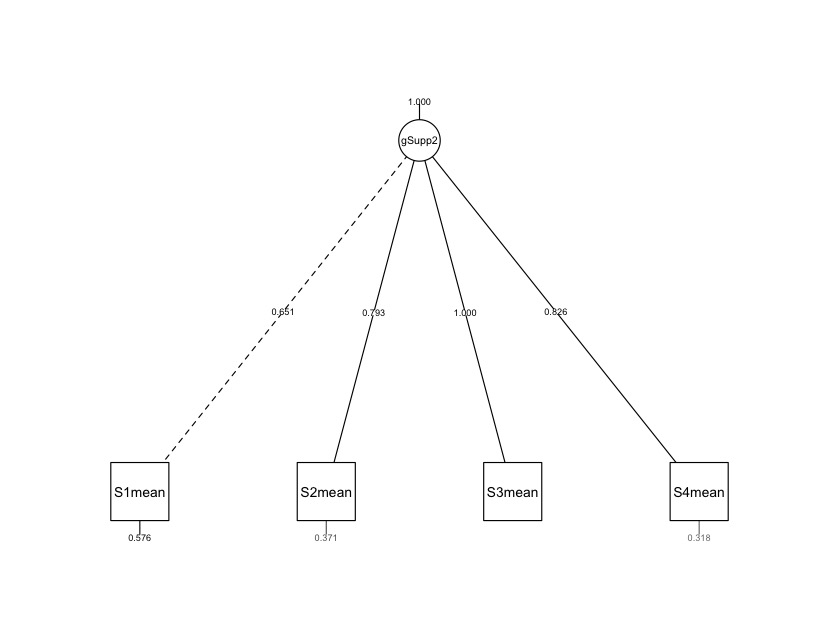
\includegraphics[width=0.8\textwidth]{../jpg/sscongeneric}
	\caption[CFA Platzhalter Test]{Modell 1: Kongenerisches Messmodell der \gls{ssauf}. Eingezeichnet sind die standardisierten Koeffizienten.}
	\label{fig:SScongeneric}
\end{figure}

\subsection{Strukturgleichungsmodell \label{subsec:Strukturgleichungsmodell}}

Trotz des schlechten kongenerischen Modell-Fits von Modell 1 wurde das Messmodell mit dem \gls{gfaktor} aus dem \gls{bist} in Verbindung gebracht (Modell 2). Das theoretische Modell bildete die empirischen Daten schlecht ab [$\upchi^2(13)=123.88$, $p<.001$, $\textnormal{CFI}=.85$, $\textnormal{RMSEA}=.22$, $\textnormal{SRMR}=.06$]. Die explizite Modellierung des Messfehlers mittels Strukturgleichungsmodell führte im Unterschied zur Analyse auf manifester Ebene dazu, dass ein moderat negativer Zusammenhang zwischen der \gls{ssauf} und psychometrischer Intelligenz festgestellt werden konnte. Die aus den vier Bedingungen der \gls{ssauf} extrahierte latente Variable sagte den \gls{gfaktor} aus dem \gls{bist} mit einem Regressionskoeffizienten $\upbeta~=~-.23$ ($p~=~.01$) vorher (siehe Abbildung \ref{fig:SSglatent}).
Eine bessere Wahrnehmungsleistung in der \gls{ssauf} (d.h. tiefere Wahrnehmungsschwellen) war folglich mit besserer kognitiver Leistung im \gls{bist} verbunden.


\begin{figure}[htbp]
	\centering
	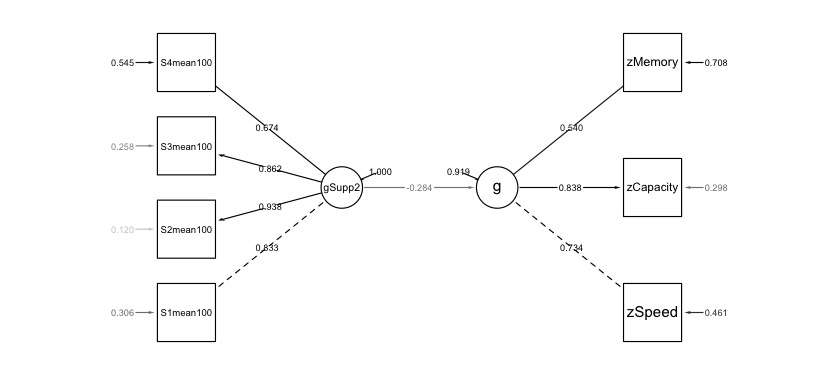
\includegraphics[width=\textwidth]{../jpg/supp-g}
	\caption[CFA Platzhalter Test]{Modell 2: Latenter Zusammenhang zwischen der \gls{ssauf} und dem \gls{gfaktor} des \gls{bist}. Eingezeichnet sind die standardisierten Koeffizienten.}
	\label{fig:SSglatent}
\end{figure} 















\section{4. Fragestellung \label{sec:4Fragestellung}}

\subsection{Fixed-Links-Messmodell der \gls{ssauf} \label{subsec:flss}}

Für die Beantwortung der vierten Fragestellung wurde versucht, die Varianzen und Kovarianzen der vier Spatial-Suppression-Bedingungen mit einem \gls{flm} zu beschreiben. Weil die Aufgabe bisher noch nie mit einem \gls{flm} beschrieben wurde, wurden unterschiedliche Modelle getestet und miteinander verglichen. Bei allen berechneten Modellen wurden zwei voneinander unabhängige latente Variablen angenommen: 
Die erste latente Variable beinhaltete aufgabenrelevante Prozesse, deren Einflüsse sich über die vier Bedingungen hinweg nicht geändert haben. In allen Messmodellen wurde dieser gleichbleibende Einfluss hergestellt, indem die unstandardisierten Faktorladungen aller manifesten Variablen auf denselben Wert (1) fixiert wurden. Weil mit diesen Fixierungen der Einfluss der in der latenten Variable abgebildeten Prozesse über die vier Bedingungen konstant gehalten wird, wird diese latente Variable im Folgenden \textit{konstante} latente Variable genannt. 
Die zweite latente Variable beinhaltete aufgabenrelevante Prozesse, die durch die vier Bedingungen systematisch manipuliert wurden. Der unterschiedlich starke Einfluss der in der latenten Variable abgebildeten Prozesse auf die Bedingungen der \gls{ssauf} wurde durch sich unterscheidende unstandardisierte Faktorladungen hergestellt. Diese latente Variable wird im Folgenden \textit{dynamische} latente Variable genannt. Um die in der Diskussion folgende Interpretation der beiden latenten Variablen zu vereinfachen, wurde die konstante latente Variable in allen Messmodellen unabhängig von der dynamischen latenten Variable gehalten.

Das erste berechnete \gls{flm} (Modell 3) berücksichtigte die Tatsache, dass die Mustergrössen über die vier Bedingungen linear zunahm ($1.8^{\circ}$, $3.6^{\circ}$, $5.4^{\circ}$, $7.2^{\circ}$).
Die unstandardisierten Faktorladungen der dynamischen latenten Variable in Modell 3 wurden deshalb linear ansteigend [$y=x,\,x\in\{1, 2, 3, 4\}$] gewählt. Modell 3 bildete die empirischen Varianzen und Kovarianzen der \gls{ssauf} nicht gut ab [$\upchi^2(4)=17.32$, $p=.002$, $\textnormal{CFI}=.89$, $\textnormal{RMSEA}=.14$, $\textnormal{SRMR}=.34$]. Die Varianz der konstanten latenten Variable betrug $642.03$ ($z=6.71$, $p<.001$) und die Varianz der dynamischen latenten Variable betrug $253.50$ ($z=4.48$, $p<.001$).
Mit Modell 4 wurde das Ergebnis der exponentiellen Regression (siehe Abschnitt \ref{sec:2Fragestellung}) berücksichtigt, welches auf manifester Ebene eine Steigung von $b=0.102$ ergeben hat. Die unstandardisierten Faktorladungen der dynamischen latenten Variable wurden deshalb mit diesem Parameter [$y=e^{0.102x},\,x\in\{1, 2, 3, 4\}$] gebildet. Das Modell konnte nicht interpretiert werden, weil die Varianz der konstanten latenten Variable negativ war.

Nach diesen zwei Modellen, welche klare Annahmen über den Verlauf der Faktorladungen der dynamischen latenten Variable machten, wurden als nächstes explorativ Verläufe von Faktorladungen gesucht, welche die empirischen Daten bestmöglich beschreiben.  In Modell 5 wurde der lineare Ladungsverlauf der dynamischen latenten Variable von Modell 3 beibehalten, die erste Bedingung aber auf $0$ gesetzt [$y=x,\,x\in\{0,1,2,3\}$]. Dieses Modell konnte nicht interpretiert werden, weil die $1.8^{\circ}$-Bedingung eine negative Fehlervarianz aufwies.
In Modell 6 wiesen die Faktorladungen der dynamischen latenten Variable einen logarithmischen Verlauf [$y=\log_{e}x,\,x\in\{1, 2, 3, 4\}$] auf. Auch diese Modell konnte aufgrund einer negativen Fehlervarianz nicht interpretiert werden. Im Gegensatz zu Modell 5 wies in Modell 6 aber die $1.8^{\circ}$-Bedingung eine negative Fehlervarianz auf.
Die Faktorladungen der dynamische latente Variable von Modell 7 wurden mit einer exponentiellen Funktion [$y=2^x,\,x\in\{1, 2, 3, 4\}$] bestimmt. Dieses Modell bildete die empirischen Daten akzeptabel ab [$\upchi^2(4)=6.61$, $p=.16$, $\textnormal{CFI}=.98$, $\textnormal{RMSEA}~=~.06$, $\textnormal{SRMR}~=~.12$]. Zwar wurde der \gls{cst} nicht signifikant, das \gls{srmr} zeigte aber an, dass die durchschnittlichen Korrelationsresiduen der manifesten Variablen hoch sind. Die Varianz der konstanten latenten Variable betrug $604.08$ ($z~=~6.92$, $p~<.001$) und die Varianz der dynamischen latenten Variable betrug $25.47$ ($z~=~3.56$, $p~<~.001$).
Nach Inspektion von Modell 7 wurde der Ladungsverlauf der dynamischen latenten Variable von Modell 8 getestet. In Modell 8 wurde ein quadratischer Ladungsverlauf [$y=x^2,\,x\in\{1, 2, 3, 4\}$] eingesetzt. Das Modell (siehe Abbildung \ref{fig:ssfl})
\begin{figure}[htb]
	\centering
	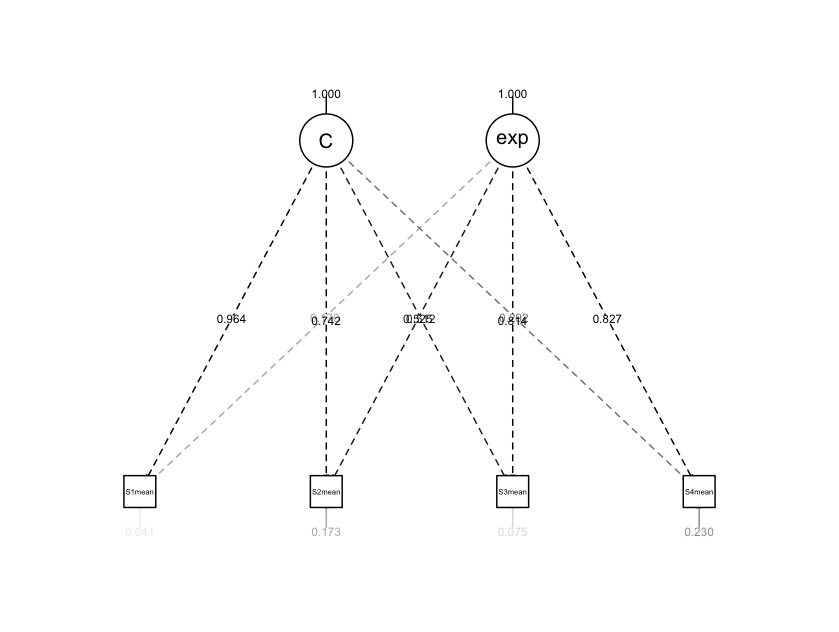
\includegraphics[width=\textwidth]{../jpg/ssfl}
	\caption[CFA Platzhalter Test]{Modell 8: \gls{flm} der \gls{ssauf}. Eingezeichnet sind die standardisierten Koeffizienten.}
	\label{fig:ssfl}
\end{figure} 
bildete die empirischen Daten gut ab [$\upchi^2(4)=4.22$, $p=.38$, $\textnormal{CFI}=1$, $\textnormal{RMSEA}~=~.02$, $\textnormal{SRMR}~=~.06$]. Der \gls{cst} war nicht signifikant und alle Fit-Indizes (auch das SRMR) zeigten ein gutes Modell an. Die Varianz der konstanten latenten Variable betrug $647.14$ ($z~=~7.43$, $p~<.001$) und die Varianz der dynamischen latenten Variable betrug $20.24$ ($z~=~3.74$, $p~<~.001$). Um den relativen Einfluss der beiden latenten Variablen auf die manifesten Variablen zu bestimmen, wurden die beiden geschätzten Varianzen skaliert \citep{Schweizer2011a}. Nach Skalierung der Varianzen betrug die Varianz der konstanten latenten Variable $647.14$ ($z~=~7.43$, $p~<.001$) und die Varianz der dynamischen latenten Variable $1790.82$ ($z~=~3.74$, $p~<~.001$). Die in der dynamischen latenten Variable gebundenen Prozesse sind folglich für die Bearbeitung der \gls{ssauf} fast drei Mal so wichtig wie die in der konstanten latenten Variable gebundenen Prozesse. Weil Modell 8 die empirischen Daten am besten abbildete, wurde für alle weiteren Berechnungen Modell 8 verwendet. Eine Übersicht über alle \gls{flm}e der \gls{ssauf} gibt Tabelle \ref{tab:ssflm}.

\begin{table}[htbp]
	%\flushleft
	\centering
	\captionsetup{labelsep = none}
	\caption[Konfirmatorische Faktorenanalyse]{\newline  \textit{Übersicht über die berichteten Fixed-Links-Modelle der \gls{ssauf}} \vspace{.2cm}}
	\label{tab:ssflm}
	%	\resizebox{\columnwidth}{!}{%	
	\begin{threeparttable}
		
		
		\begin{tabular}{
				S[table-format = 1.0, table-space-text-post = $^{*a}$]
				l
				S[table-format = 2.2]
				S[table-format = 1.0]
				S[table-format = 0.3, add-integer-zero=false]
				S[table-format = 1.2, add-integer-zero=false]
				S[table-format = 0.2, add-integer-zero=false]
				S[table-format = 0.2, add-integer-zero=false]
				%				S[table-format = 1.2, add-integer-zero=false]
			}
			
			\hline
			{Modell}		& Ladungsverlauf		& 	{$\upchi^2$}	& \textit{df}	& {\textit{p}}	&	{\textnormal{CFI}} 	&	{\textnormal{RMSEA}}	&	{\textnormal{SRMR}}\\
			\hline
			
			%			1			&	SS kongenerisch	&	28.44		&	2			&	<.001			&	.78		&	.27					&	.09	\\
			%			2			&	SGM				&	91.06	&	13			&	<.001			&	.77		&	.19					&	.06	\\
			3	&	 $y=x$			&	17.32	&	4	&	.002	&	.89		&	.14		&	.34	\\
			4{$^{*}$}	&	$y=e^{0.102x}$	&	{\textemdash}		&	{\textemdash}	&	{\textemdash}		&	{\textemdash}		&	{\textemdash}		&	{\textemdash}	\\
			5{$^{*}$}	&	$y=x$			&	{\textemdash}		&	{\textemdash}	&	{\textemdash}		&	{\textemdash}		&	{\textemdash}		&	{\textemdash}	\\
			6{$^{*}$}	&	$y=\log_e x$	&	{\textemdash}		&	{\textemdash}	&	{\textemdash}		&	{\textemdash}		&	{\textemdash}		&	{\textemdash}	\\
			7			&	$y=2^x$			&	6.61	&	4	&	.16		&	.98		&	.06		&	.12	\\
			8			&	$y=x^2$			&	4.22	&	4	&	.38		&	1.00	&	.02		&	.06	\\
			\hline
			
			
		\end{tabular}%
		%}
		\begin{tablenotes}[flushleft]
			\footnotesize				% font size
			\setlength\labelsep{0pt}	% no indent on second line
			\item \textit{Anmerkungen.} Der Ladungsverlauf bezieht sich auf die unstandardisierten Faktorladungen der dynamischen latenten Variable. Die unstandardisierten Faktorladungen der konstanten latenten Variable betrugen immer $1$. Es gilt für alle Funktionen $x\in\{1,2,3,4\}$ (ausgenommen Modell 5, in welchem $x\in\{0,1,2,3\}$). $\upchi^2 =$ Satorra-Bentler \citeyearpar{Satorra1994} korrigierter $\upchi^2$-Wert. \textit{df} = Freiheitsgrade. \gls{cfi} = comparative fit index. \gls{rmsea} = root mean square error of approximation. \gls{srmr} = standardized root mean square residual.
			%\item {$^{a}$} Die Fehlervarianz der $5.4^{\circ}$-Bedingung wurde gezwungen, keinen negative Werte anzunehmen.
			\item {$^{*}$} Das Modell konnte nicht interpretiert werden, weil eine geschätzte Varianz negativ war.

		\end{tablenotes}%
	\end{threeparttable}%
	%}
\end{table}





\subsection{Strukturgleichungsmodell}

Modell 8 wurde mit dem \gls{gfaktor} aus dem \gls{bist} in Verbindung gebracht (Modell 9; siehe Abbildung \ref{fig:ssflg}).
Das Modell bildete die empirischen Daten gut ab [$\upchi^2(14)=14.03$, $p=.45$, $\textnormal{CFI}=1$, $\textnormal{RMSEA}~=~.00$, $\textnormal{SRMR}~=~.05$]. Die konstante latente Variable sagte den \gls{gfaktor} mit $\upbeta~=~-.24$ ($p~=~.03$) und die dynamische latente Variable den \gls{gfaktor} mit $\upbeta~=~-.14$ ($p~=~.13$) vorher.

\begin{figure}[htb]
	\centering
	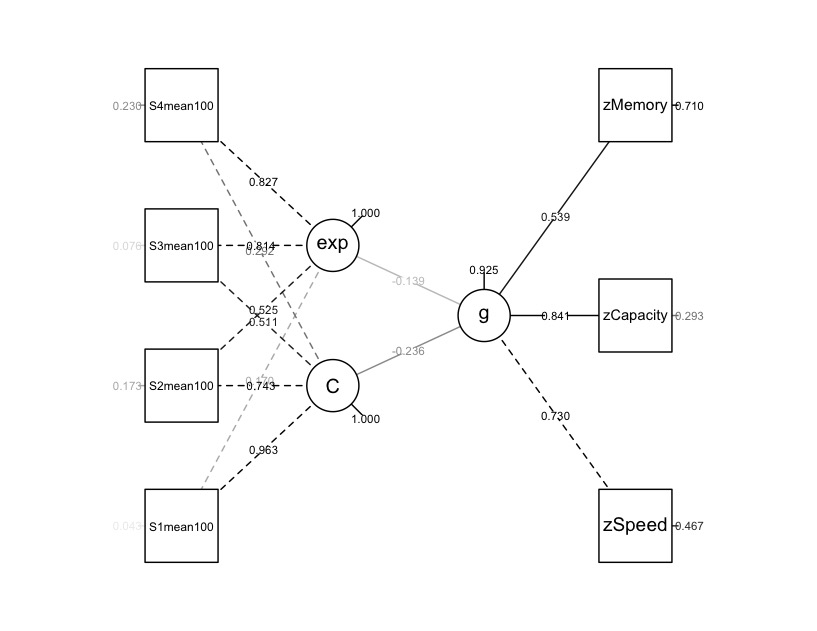
\includegraphics[width=\textwidth]{../jpg/ssflg}
	\caption[CFA Platzhalter Test]{Modell 9: Latenter Zusammenhang zwischen dem \gls{flm} der \gls{ssauf} und dem \gls{gfaktor} aus dem \gls{bist}. Eingezeichnet sind die standardisierten Koeffizienten.\\
	$^{*}~p~<~.05$. $^{**}~p~<~.01$. $^{***}~p~<~.001$.
	
	}
	\label{fig:ssflg}
\end{figure} 









\clearpage
\section{5. Fragestellung}

Der Zusammenhang der \gls{ssauf} mit der \gls{ha} und dem \gls{bist} wurde zum einen auf manifester Ebene und zum anderen auf latenter Ebene bestimmt. 

\subsection{Analyse auf manifester Ebene}

In einem ersten Schritt wurden die vier Bedingungen der \gls{ssauf}, die vier Bedingungen der \gls{ha} und der \textit{z}-Wert des \gls{bist} miteinander korreliert. Tabelle \ref{tab:shzmanifest} gibt eine Übersicht über die Resultate dieser korrelativen Analyse. Es korrelierten nur die $3.6^{\circ}$-Bedingung ($r_{s}~=~.20$, $p~=~.006$) und die $5.4^{\circ}$-Bedingung ($r_{s}~=~.17$, $p~=~.024$) mit der 0-bit Bedingung der \gls{ha}. Alle restlichen Zusammenhänge zwischen der \gls{ssauf} und der \gls{ha} waren nicht signifikant.
Die vier Bedingungen der \gls{ha} hingegen korrelierten alle signifikant mit dem \textit{z}-Wert (siehe Tabelle \ref{tab:shzmanifest}).




In einem zweiten Schritt wurden die vier \glspl{rz} der \gls{ha} mit einer linearen Regression der Form $y=a+bx$ vorhergesagt (siehe Abbildung \ref{fig:linmodel}). Deskriptive Angaben zu den daraus resultierenden Parametern $a$, dem Achsenabschnitt, und $b$, der Steigung, sind in Tabelle \ref{tab:InterSlope} zu finden. Über alle \glspl{vp} gemittelt betrug $R^2=.96$, wobei im Gegensatz zur regressionsanalytischen Analyse der \gls{ssauf} (siehe Abschnitt \ref{sec:2Fragestellung}) geringere individuelle Variabilität (\gls{sd} $=.04$, Min = .732, Max = .999) bestand.
\begin{figure}[b]
	\centering
	\resizebox{\textwidth}{!}{

% Created by tikzDevice version 0.10.1 on 2016-06-01 11:19:08
% !TEX encoding = UTF-8 Unicode
\begin{tikzpicture}[x=1pt,y=1pt]
\definecolor{fillColor}{RGB}{255,255,255}
\path[use as bounding box,fill=fillColor,fill opacity=0.00] (0,0) rectangle (505.89,505.89);
\begin{scope}
\path[clip] ( 54.00, 78.00) rectangle (451.89,475.89);
\definecolor{drawColor}{RGB}{0,0,0}

\path[draw=drawColor,line width= 0.4pt,line join=round,line cap=round] (  0.00, 91.24) --
(  1.19, 92.21) --
(  2.42, 93.20) --
(  3.65, 94.20) --
(  4.88, 95.19) --
(  6.11, 96.18) --
(  7.33, 97.18) --
(  8.56, 98.17) --
(  9.79, 99.17) --
( 11.02,100.16) --
( 12.25,101.15) --
( 13.47,102.15) --
( 14.70,103.14) --
( 15.93,104.14) --
( 17.16,105.13) --
( 18.39,106.12) --
( 19.61,107.12) --
( 20.84,108.11) --
( 22.07,109.11) --
( 23.30,110.10) --
( 24.53,111.09) --
( 25.75,112.09) --
( 26.98,113.08) --
( 28.21,114.08) --
( 29.44,115.07) --
( 30.67,116.06) --
( 31.90,117.06) --
( 33.12,118.05) --
( 34.35,119.05) --
( 35.58,120.04) --
( 36.81,121.03) --
( 38.04,122.03) --
( 39.26,123.02) --
( 40.49,124.02) --
( 41.72,125.01) --
( 42.95,126.00) --
( 44.18,127.00) --
( 45.40,127.99) --
( 46.63,128.99) --
( 47.86,129.98) --
( 49.09,130.97) --
( 50.32,131.97) --
( 51.54,132.96) --
( 52.77,133.96) --
( 54.00,134.95) --
( 55.23,135.94) --
( 56.46,136.94) --
( 57.68,137.93) --
( 58.91,138.93) --
( 60.14,139.92) --
( 61.37,140.91) --
( 62.60,141.91) --
( 63.82,142.90) --
( 65.05,143.90) --
( 66.28,144.89) --
( 67.51,145.88) --
( 68.74,146.88) --
( 69.96,147.87) --
( 71.19,148.87) --
( 72.42,149.86) --
( 73.65,150.85) --
( 74.88,151.85) --
( 76.10,152.84) --
( 77.33,153.83) --
( 78.56,154.83) --
( 79.79,155.82) --
( 81.02,156.82) --
( 82.25,157.81) --
( 83.47,158.80) --
( 84.70,159.80) --
( 85.93,160.79) --
( 87.16,161.79) --
( 88.39,162.78) --
( 89.61,163.77) --
( 90.84,164.77) --
( 92.07,165.76) --
( 93.30,166.76) --
( 94.53,167.75) --
( 95.75,168.74) --
( 96.98,169.74) --
( 98.21,170.73) --
( 99.44,171.73) --
(100.67,172.72) --
(101.89,173.71) --
(103.12,174.71) --
(104.35,175.70) --
(105.58,176.70) --
(106.81,177.69) --
(108.03,178.68) --
(109.26,179.68) --
(110.49,180.67) --
(111.72,181.67) --
(112.95,182.66) --
(114.17,183.65) --
(115.40,184.65) --
(116.63,185.64) --
(117.86,186.64) --
(119.09,187.63) --
(120.31,188.62) --
(121.54,189.62) --
(122.77,190.61) --
(124.00,191.61) --
(125.23,192.60) --
(126.46,193.59) --
(127.68,194.59) --
(128.91,195.58) --
(130.14,196.58) --
(131.37,197.57) --
(132.60,198.56) --
(133.82,199.56) --
(135.05,200.55) --
(136.28,201.55) --
(137.51,202.54) --
(138.74,203.53) --
(139.96,204.53) --
(141.19,205.52) --
(142.42,206.52) --
(143.65,207.51) --
(144.88,208.50) --
(146.10,209.50) --
(147.33,210.49) --
(148.56,211.49) --
(149.79,212.48) --
(151.02,213.47) --
(152.24,214.47) --
(153.47,215.46) --
(154.70,216.46) --
(155.93,217.45) --
(157.16,218.44) --
(158.38,219.44) --
(159.61,220.43) --
(160.84,221.43) --
(162.07,222.42) --
(163.30,223.41) --
(164.52,224.41) --
(165.75,225.40) --
(166.98,226.39) --
(168.21,227.39) --
(169.44,228.38) --
(170.67,229.38) --
(171.89,230.37) --
(173.12,231.36) --
(174.35,232.36) --
(175.58,233.35) --
(176.81,234.35) --
(178.03,235.34) --
(179.26,236.33) --
(180.49,237.33) --
(181.72,238.32) --
(182.95,239.32) --
(184.17,240.31) --
(185.40,241.30) --
(186.63,242.30) --
(187.86,243.29) --
(189.09,244.29) --
(190.31,245.28) --
(191.54,246.27) --
(192.77,247.27) --
(194.00,248.26) --
(195.23,249.26) --
(196.45,250.25) --
(197.68,251.24) --
(198.91,252.24) --
(200.14,253.23) --
(201.37,254.23) --
(202.59,255.22) --
(203.82,256.21) --
(205.05,257.21) --
(206.28,258.20) --
(207.51,259.20) --
(208.73,260.19) --
(209.96,261.18) --
(211.19,262.18) --
(212.42,263.17) --
(213.65,264.17) --
(214.88,265.16) --
(216.10,266.15) --
(217.33,267.15) --
(218.56,268.14) --
(219.79,269.14) --
(221.02,270.13) --
(222.24,271.12) --
(223.47,272.12) --
(224.70,273.11) --
(225.93,274.11) --
(227.16,275.10) --
(228.38,276.09) --
(229.61,277.09) --
(230.84,278.08) --
(232.07,279.08) --
(233.30,280.07) --
(234.52,281.06) --
(235.75,282.06) --
(236.98,283.05) --
(238.21,284.05) --
(239.44,285.04) --
(240.66,286.03) --
(241.89,287.03) --
(243.12,288.02) --
(244.35,289.02) --
(245.58,290.01) --
(246.80,291.00) --
(248.03,292.00) --
(249.26,292.99) --
(250.49,293.98) --
(251.72,294.98) --
(252.94,295.97) --
(254.17,296.97) --
(255.40,297.96) --
(256.63,298.95) --
(257.86,299.95) --
(259.09,300.94) --
(260.31,301.94) --
(261.54,302.93) --
(262.77,303.92) --
(264.00,304.92) --
(265.23,305.91) --
(266.45,306.91) --
(267.68,307.90) --
(268.91,308.89) --
(270.14,309.89) --
(271.37,310.88) --
(272.59,311.88) --
(273.82,312.87) --
(275.05,313.86) --
(276.28,314.86) --
(277.51,315.85) --
(278.73,316.85) --
(279.96,317.84) --
(281.19,318.83) --
(282.42,319.83) --
(283.65,320.82) --
(284.87,321.82) --
(286.10,322.81) --
(287.33,323.80) --
(288.56,324.80) --
(289.79,325.79) --
(291.01,326.79) --
(292.24,327.78) --
(293.47,328.77) --
(294.70,329.77) --
(295.93,330.76) --
(297.15,331.76) --
(298.38,332.75) --
(299.61,333.74) --
(300.84,334.74) --
(302.07,335.73) --
(303.30,336.73) --
(304.52,337.72) --
(305.75,338.71) --
(306.98,339.71) --
(308.21,340.70) --
(309.44,341.70) --
(310.66,342.69) --
(311.89,343.68) --
(313.12,344.68) --
(314.35,345.67) --
(315.58,346.67) --
(316.80,347.66) --
(318.03,348.65) --
(319.26,349.65) --
(320.49,350.64) --
(321.72,351.64) --
(322.94,352.63) --
(324.17,353.62) --
(325.40,354.62) --
(326.63,355.61) --
(327.86,356.61) --
(329.08,357.60) --
(330.31,358.59) --
(331.54,359.59) --
(332.77,360.58) --
(334.00,361.57) --
(335.22,362.57) --
(336.45,363.56) --
(337.68,364.56) --
(338.91,365.55) --
(340.14,366.54) --
(341.36,367.54) --
(342.59,368.53) --
(343.82,369.53) --
(345.05,370.52) --
(346.28,371.51) --
(347.51,372.51) --
(348.73,373.50) --
(349.96,374.50) --
(351.19,375.49) --
(352.42,376.48) --
(353.65,377.48) --
(354.87,378.47) --
(356.10,379.47) --
(357.33,380.46) --
(358.56,381.45) --
(359.79,382.45) --
(361.01,383.44) --
(362.24,384.44) --
(363.47,385.43) --
(364.70,386.42) --
(365.93,387.42) --
(367.15,388.41) --
(368.38,389.41) --
(369.61,390.40) --
(370.84,391.39) --
(372.07,392.39) --
(373.29,393.38) --
(374.52,394.38) --
(375.75,395.37) --
(376.98,396.36) --
(378.21,397.36) --
(379.43,398.35) --
(380.66,399.35) --
(381.89,400.34) --
(383.12,401.33) --
(384.35,402.33) --
(385.57,403.32) --
(386.80,404.32) --
(388.03,405.31) --
(389.26,406.30) --
(390.49,407.30) --
(391.72,408.29) --
(392.94,409.29) --
(394.17,410.28) --
(395.40,411.27) --
(396.63,412.27) --
(397.86,413.26) --
(399.08,414.26) --
(400.31,415.25) --
(401.54,416.24) --
(402.77,417.24) --
(404.00,418.23) --
(405.22,419.23) --
(406.45,420.22) --
(407.68,421.21) --
(408.91,422.21) --
(410.14,423.20) --
(411.36,424.20) --
(412.59,425.19) --
(413.82,426.18) --
(415.05,427.18) --
(416.28,428.17) --
(417.50,429.17) --
(418.73,430.16) --
(419.96,431.15) --
(421.19,432.15) --
(422.42,433.14) --
(423.64,434.13) --
(424.87,435.13) --
(426.10,436.12) --
(427.33,437.12) --
(428.56,438.11) --
(429.78,439.10) --
(431.01,440.10) --
(432.24,441.09) --
(433.47,442.09) --
(434.70,443.08) --
(435.93,444.07) --
(437.15,445.07) --
(438.38,446.06) --
(439.61,447.06) --
(440.84,448.05) --
(442.07,449.04) --
(443.29,450.04) --
(444.52,451.03) --
(445.75,452.03) --
(446.98,453.02) --
(448.21,454.01) --
(449.43,455.01) --
(450.66,456.00) --
(451.89,457.00) --
(453.12,457.99) --
(454.35,458.98) --
(455.57,459.98) --
(456.80,460.97) --
(458.03,461.97) --
(459.26,462.96) --
(460.49,463.95) --
(461.71,464.95) --
(462.94,465.94) --
(464.17,466.94) --
(465.40,467.93) --
(466.63,468.92) --
(467.85,469.92) --
(469.08,470.91) --
(470.31,471.91) --
(471.54,472.90) --
(472.77,473.89) --
(473.99,474.89) --
(475.22,475.88) --
(476.45,476.88) --
(477.68,477.87) --
(478.91,478.86) --
(480.14,479.86) --
(481.36,480.85) --
(482.59,481.85) --
(483.82,482.84) --
(485.05,483.83) --
(486.28,484.83) --
(487.50,485.82) --
(488.73,486.82) --
(489.96,487.81) --
(491.19,488.80) --
(492.42,489.80) --
(493.64,490.79) --
(494.87,491.79) --
(496.10,492.78) --
(497.33,493.77) --
(498.56,494.77) --
(499.78,495.76) --
(501.01,496.76) --
(502.24,497.75) --
(503.47,498.74) --
(504.70,499.74) --
(505.89,500.70);
\end{scope}
\begin{scope}
\path[clip] (  0.00,  0.00) rectangle (505.89,505.89);
\definecolor{drawColor}{RGB}{0,0,0}

\node[text=drawColor,anchor=base,inner sep=0pt, outer sep=0pt, scale=  1.20] at (252.94, 32.40) {Bits ($\log_{2}\textnormal{n}$)};

\node[text=drawColor,rotate= 90.00,anchor=base,inner sep=0pt, outer sep=0pt, scale=  1.20] at ( 15.60,276.94) {Reaktionszeit (ms)};
\end{scope}
\begin{scope}
\path[clip] (  0.00,  0.00) rectangle (505.89,505.89);
\definecolor{drawColor}{RGB}{0,0,0}

\path[draw=drawColor,line width= 0.4pt,line join=round,line cap=round] ( 68.74, 78.00) -- (437.15, 78.00);

\path[draw=drawColor,line width= 0.4pt,line join=round,line cap=round] ( 68.74, 78.00) -- ( 68.74, 72.00);

\path[draw=drawColor,line width= 0.4pt,line join=round,line cap=round] (191.54, 78.00) -- (191.54, 72.00);

\path[draw=drawColor,line width= 0.4pt,line join=round,line cap=round] (314.35, 78.00) -- (314.35, 72.00);

\path[draw=drawColor,line width= 0.4pt,line join=round,line cap=round] (437.15, 78.00) -- (437.15, 72.00);

\node[text=drawColor,anchor=base,inner sep=0pt, outer sep=0pt, scale=  1.20] at ( 68.74, 60.00) {0};

\node[text=drawColor,anchor=base,inner sep=0pt, outer sep=0pt, scale=  1.20] at (191.54, 60.00) {1};

\node[text=drawColor,anchor=base,inner sep=0pt, outer sep=0pt, scale=  1.20] at (314.35, 60.00) {2};

\node[text=drawColor,anchor=base,inner sep=0pt, outer sep=0pt, scale=  1.20] at (437.15, 60.00) {2.58};

\path[draw=drawColor,line width= 0.4pt,line join=round,line cap=round] ( 54.00, 92.74) -- ( 54.00,461.15);

\path[draw=drawColor,line width= 0.4pt,line join=round,line cap=round] ( 54.00, 92.74) -- ( 48.00, 92.74);

\path[draw=drawColor,line width= 0.4pt,line join=round,line cap=round] ( 54.00,166.42) -- ( 48.00,166.42);

\path[draw=drawColor,line width= 0.4pt,line join=round,line cap=round] ( 54.00,240.10) -- ( 48.00,240.10);

\path[draw=drawColor,line width= 0.4pt,line join=round,line cap=round] ( 54.00,313.79) -- ( 48.00,313.79);

\path[draw=drawColor,line width= 0.4pt,line join=round,line cap=round] ( 54.00,387.47) -- ( 48.00,387.47);

\path[draw=drawColor,line width= 0.4pt,line join=round,line cap=round] ( 54.00,461.15) -- ( 48.00,461.15);

\node[text=drawColor,anchor=base east,inner sep=0pt, outer sep=0pt, scale=  1.20] at ( 45.60, 88.60) {200};

\node[text=drawColor,anchor=base east,inner sep=0pt, outer sep=0pt, scale=  1.20] at ( 45.60,162.29) {250};

\node[text=drawColor,anchor=base east,inner sep=0pt, outer sep=0pt, scale=  1.20] at ( 45.60,235.97) {300};

\node[text=drawColor,anchor=base east,inner sep=0pt, outer sep=0pt, scale=  1.20] at ( 45.60,309.65) {350};

\node[text=drawColor,anchor=base east,inner sep=0pt, outer sep=0pt, scale=  1.20] at ( 45.60,383.34) {400};

\node[text=drawColor,anchor=base east,inner sep=0pt, outer sep=0pt, scale=  1.20] at ( 45.60,457.02) {450};
\end{scope}
\begin{scope}
\path[clip] ( 54.00, 78.00) rectangle (451.89,475.89);
\definecolor{drawColor}{RGB}{0,0,0}
\definecolor{fillColor}{RGB}{0,0,0}

\path[draw=drawColor,line width= 0.4pt,line join=round,line cap=round,fill=fillColor] ( 68.74,151.84) circle (  2.25);

\path[draw=drawColor,line width= 0.4pt,line join=round,line cap=round,fill=fillColor] (191.54,234.94) circle (  2.25);

\path[draw=drawColor,line width= 0.4pt,line join=round,line cap=round,fill=fillColor] (314.35,353.59) circle (  2.25);

\path[draw=drawColor,line width= 0.4pt,line join=round,line cap=round,fill=fillColor] (437.15,443.70) circle (  2.25);

\path[draw=drawColor,line width= 0.4pt,line join=round,line cap=round] ( 68.74,148.62) -- ( 68.74,155.06);

\path[draw=drawColor,line width= 0.4pt,line join=round,line cap=round] ( 65.12,148.62) --
( 68.74,148.62) --
( 72.35,148.62);

\path[draw=drawColor,line width= 0.4pt,line join=round,line cap=round] ( 72.35,155.06) --
( 68.74,155.06) --
( 65.12,155.06);

\path[draw=drawColor,line width= 0.4pt,line join=round,line cap=round] (191.54,231.43) -- (191.54,238.45);

\path[draw=drawColor,line width= 0.4pt,line join=round,line cap=round] (187.93,231.43) --
(191.54,231.43) --
(195.16,231.43);

\path[draw=drawColor,line width= 0.4pt,line join=round,line cap=round] (195.16,238.45) --
(191.54,238.45) --
(187.93,238.45);

\path[draw=drawColor,line width= 0.4pt,line join=round,line cap=round] (314.35,347.62) -- (314.35,359.56);

\path[draw=drawColor,line width= 0.4pt,line join=round,line cap=round] (310.73,347.62) --
(314.35,347.62) --
(317.96,347.62);

\path[draw=drawColor,line width= 0.4pt,line join=round,line cap=round] (317.96,359.56) --
(314.35,359.56) --
(310.73,359.56);

\path[draw=drawColor,line width= 0.4pt,line join=round,line cap=round] (437.15,436.20) -- (437.15,451.20);

\path[draw=drawColor,line width= 0.4pt,line join=round,line cap=round] (433.54,436.20) --
(437.15,436.20) --
(440.77,436.20);

\path[draw=drawColor,line width= 0.4pt,line join=round,line cap=round] (440.77,451.20) --
(437.15,451.20) --
(433.54,451.20);
\end{scope}
\end{tikzpicture}




%
}
\caption[Lineare Regression der \gls{ha}]{Linearer Einfluss der Anzahl Bits auf die Reaktionszeit in der \gls{ha}. Eingezeichnet sind die Mittelwerte $\pm$ Standardfehler der Mittelwerte. $y = 237 + 67x $, $R^2=.96$. n = Anzahl Antwortalternativen.}
\label{fig:linmodel}
\end{figure}
\begin{table}[htbp]
	%\flushleft
	\centering
	\captionsetup{labelsep = none}
	\caption[Deskriptive Angaben zur ]{\newline  \textit{Deskriptive Angaben zur linearen Regression ($y=a+bx$) für die Vorhersage der Reaktionszeiten durch die Anzahl Antwortalternativen in der \gls{ha}} \vspace{.2cm}}
	\label{tab:InterSlope}
	%	\resizebox{\columnwidth}{!}{%	
	\begin{threeparttable}
		
		\begin{tabular}{
				c
				S[table-format = 3.0]
				S[table-format = 2.0]
				S[table-format = 3.0]
				S[table-format = 3.0]
				S[table-format = 1.2]
				S[table-format = 1.2]
				%				S[table-format = 1.2, add-integer-zero=false]
			}
			
			\hline
			& 	\multicolumn{4}{c}{in Millisekunden}	&		&				\\
			
			\cline{2-5}
			Parameter	& 	{\textit{M}}	&{\textit{SD}}	&	{Min}	&	{Max} 	&	{\textnormal{Schiefe}}	&	{\textnormal{Kurtosis}}\\% &S-W \textit{p}-Wert\\
			\hline
			\textit{a}	&		237			&	28			&	177		&	350		&	1.13					&	2.64	\\%				& 		$.008$			\\
			\textit{b}	&		67			&	80			&	28		&	121		&	0.53					&	-0.18	\\%				& 		$<.001$			\\
			%			&&&&&&\\
			%			$R^2$			&	.01		&	.80			&	.25			&	1.00	&	&\\
			
			
			\hline
		\end{tabular}%
		%}
		\begin{tablenotes}[flushleft]
			\footnotesize				% font size
			\setlength\labelsep{0pt}	% no indent on second line
			\item \textit{Anmerkungen.} \textit{a}~=~Achsenabschnitt, \textit{b}~=~Steigung, Min~=~Minimum, Max~=Maximum.
		\end{tablenotes}%
	\end{threeparttable}%
	%}
\end{table}
Während der Achsenabschnitt ($a~=~237$) gering mit dem \textit{z}-Wert aus dem \gls{bist} korrelierte ($r_{s}~=~-.16$, $p~=~.03$), zeigte die Steigung ($b~=~67$) eine mittlere Korrelation  mit dem \textit{z}-Wert ($r_{s}~=~-.26$, $p~<~.001$).

Für die letzte Analyse auf manifester Ebene wurden die regressionsanalytisch hergeleiteten Parameter der \gls{ssauf} und der \gls{ha} mit dem \textit{z}-Wert aus dem \gls{bist} in Zusammenhang gesetzt. Die Analyse zeigte, dass die regressionsanalytisch abgeleitetend Parameter der \gls{ssauf} weder signifikant mit den aus der \gls{ha} abgeleiteten Parameter, noch mit dem \textit{z}-Wert des \gls{bist} signifikant korrelierten (siehe Tabelle \ref{tab:ababz}).

\begin{table}[htbp] % see http://tex.stackexchange.com/questions/247921/different-column-widths-under-a-multicolumn-prevent-appropriate-centering
	%	\flushleft
	\centering
	\captionsetup{labelsep = none}
	\caption[Korrelationen all]{\newline  \textit{Spearmans Rangkorrelationen zwischen regressionsanalytisch abgeleiteten Parametern der \gls{ssauf}, der \gls{ha} und dem \textit{z}-Wert des \gls{bist}} \vspace{.2cm}}
	\label{tab:ababz}
	%	\resizebox{1.5\columnwidth}{!}{%	
	\begin{threeparttable}
		\sisetup{table-space-text-post = $^{***}$}
		\newlength{\tempdima}
		\settowidth{\tempdima}{\gls{ssauf}}% compute width needed
		\addtolength{\tempdima}{-2\tabcolsep}% minus default column sep
		\begin{tabular}{
				p{.1cm}
				c
				S[table-format = 0.2, add-integer-zero=false]
				S[table-format = 0.2, add-integer-zero=false]
				p{.001cm}
				S[table-format = 0.2, add-integer-zero=false]
				S[table-format = 0.2, add-integer-zero=false]
				p{.001cm}
				S[table-format = 0.2, add-integer-zero=false]
				>{\centering\arraybackslash}p{1.2cm}
			}
			\hline
			
				&					& 	\multicolumn{2}{c}{\gls{ssauf}}	&	&	\multicolumn{2}{c}{\gls{ha}}	&	&	\multicolumn{1}{c}{\gls{bist}}	\\
			
			\cline{3-4}
			\cline{6-7}
			\cline{9-9}
			
				&	{Parameter}		&	{\makebox[0.5\tempdima]{1}}	&	{\makebox[0.5\tempdima]{2}}		&&	{3}				&	 {4}			&&{5}\\
			\hline
			1	&	\textit{a}		&					&			&& 					&					&&\\
			2	&	\textit{b}		&	-.67{$^{***}$}	&			&& 					&					&&\\
			\rule{0pt}{4ex}%  EXTRA vertical height
			3	&	\textit{a}		&	.14				&	.01		&&					&					&&\\
			4	&	\textit{b}		&	.04				&	-.08	&&	-.07			&					&&\\
			\rule{0pt}{4ex}%  EXTRA vertical height
			5	&	\textit{z}-Wert	&	-.13			&	.04		&&	-.16{$^{*}$}	&	-.26{$^{***}$}	&&\\

			\hline
			
		\end{tabular}%
		%}
		\begin{tablenotes}[flushleft]
			\footnotesize				% font size
			\setlength\labelsep{0pt}	% no indent on second line
			\item \textit{Anmerkungen.} \textit{a}~=~Asymptote bei der \gls{ssauf}, Achsenabschnitt bei der \gls{ha}. \textit{b}~=~Steigung. \\
			$^{*}~p~<~.05$. $^{**}~p~<~.01$. $^{***}~p~<~.001$ (zweiseitig).
		\end{tablenotes}%
	\end{threeparttable}%
	%	}
\end{table}

\clearpage
\subsection{Analyse auf latenter Ebene}

Für die Analyse der Zusammenhänge auf latenter Ebene musste für die \gls{ha} zuerst ein Fixed-Links-Messmodell gefunden werden. Dabei wurden analog zum Vorgehen in Abschnitt \ref{subsec:flss} zwei unabhängige latente Variablen angenommen, die die Varianz und Kovarianz der vier Hick-Bedingungen erklären. Die unstandardisierten Faktorladungen der konstanten latenten Variable betrug bei allen Messmodellen 1, die unstandardisierten Faktorladungen der dynamischen latenten Variable hingegen wurden variiert.

Die regressionsanalytische Analyse der \gls{ha} (siehe Abbildung \ref{fig:linmodel}) hat zwischen der Anzahl Bits und der \gls{rz} einen linearen Zusammenhang ergeben. In Modell 10 wurden die unstandardisierten Faktorladungen der dynamischen latenten Variable deshalb linear ansteigend gewählt [$y=x,\,x\in\{1, 2, 3, 4\}$]. Modell 10 bildete die empirischen Varianzen und Kovarianzen der \gls{ha} nicht gut ab [$\upchi^2(4)=37.34$, $p<.001$, $\textnormal{CFI}=.89$, $\textnormal{RMSEA}=.22$, $\textnormal{SRMR}=.17$]. Die Varianz der konstanten latenten Variable betrug $470.13$ ($z=3.81$, $p<.001$) und die Varianz der dynamischen latenten Variable betrug $186.10$ ($z=6.53$, $p<.001$).
In Modell 11 wurden die unstandardisierten Faktorladungen der dynamischen latenten Variable entsprechend der Anzahl Bit der Bedingung gewählt [$y=\log_{2}x,\,x\in\{1, 2, 4, 6\}$]. Modell 11 bildete die empirischen Varianzen und Kovarianzen der \gls{ha} ebenfalls nicht gut ab [$\upchi^2(4)=32.19$, $p<.001$, $\textnormal{CFI}=.91$, $\textnormal{RMSEA}=.20$, $\textnormal{SRMR}=.14$]. Die Varianz der konstanten latenten Variable betrug $759.80$ ($z=6.72$, $p<.001$) und die Varianz der dynamischen latenten Variable betrug $310.18$ ($z=5.74$, $p<.001$).
Modell 12 testete die Annahme, dass die Ladungen der unstandardisierten Faktorladungen der dynamischen latenten Variable entsprechend der Anzahl Antwortalternativen verlaufen [$y=x,\,x\in\{1, 2, 4, 6\}$]. Modell 12 bildete die empirischen Varianzen und Kovarianzen der \gls{ha} erstmals gut ab [$\upchi^2(4)=8.64$, $p=.07$, $\textnormal{CFI}=.99$, $\textnormal{RMSEA}=.08$, $\textnormal{SRMR}=.09$]. Die Varianz der konstanten latenten Variable betrug $559.73$ ($z=4.87$, $p<.001$) und die Varianz der dynamischen latenten Variable betrug $102.83$ ($z=7.26$, $p<.001$).

Modelle 10 bis 12 beinhalteten klare Annahmen über den Verlauf der unstandardisierten Faktorladungen der dynamischen latenten Variable. Als nächstes wurden explorativ Ladungsverläufe getestet, um die empirischen Daten bestmöglich zu beschreiben. 
In Modell 13 wiesen die Faktorladungen der dynamischen latenten Variable einen logarithmischen Verlauf [$y=\log_{e}x,\,x\in\{1, 2, 3, 4\}$] auf. Dieses Modell konnte nicht interpretiert werden, weil eine geschätzte Fehlervarianz negativ war.
Modell 14 beinhaltete einen quadratisch ansteigenden Ladungsverlauf der dynamischen latenten Variable [$y=x^2,\,x\in\{1, 2, 3, 4\}$]. Modell 14 bildete die empirischen Varianzen und Kovarianzen der \gls{ha} nicht gut ab [$\upchi^2(4)=11.36$, $p=.02$, $\textnormal{CFI}=.98$, $\textnormal{RMSEA}=.10$, $\textnormal{SRMR}=.07$]. Die Varianz der konstanten latenten Variable betrug $624.88$ ($z=5.49$, $p<.001$) und die Varianz der dynamischen latenten Variable betrug $13.53$ ($z=6.93$, $p<.001$).
Die besten Ergebnisse erzielte Modell 15, in welchem ein logistischer Ladungsverlauf der dynamischen latenten Variable eingesetzt wurde [$y={1}/({1 + e^{(-x/.8)}}),\,x\in\{-3,-1,1,3\}$]. Das theoretische Modell (siehe Abbildung \ref{fig:hafl}) 
\begin{figure}[b]
	\centering
	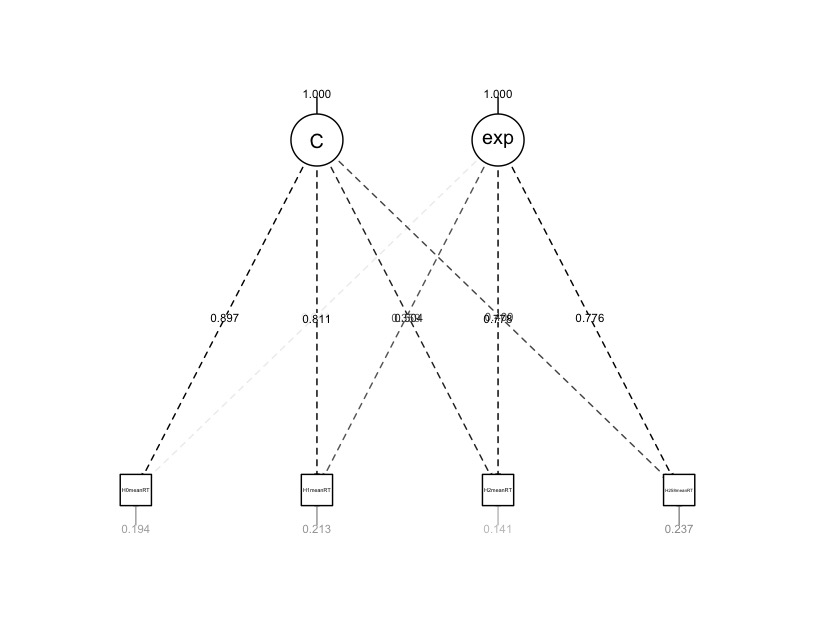
\includegraphics[width=\textwidth]{../jpg/hafl}
	\caption[CFA Platzhalter Modell 15]{Modell 15: \gls{flm} der \gls{ha}. Eingezeichnet sind die standardisierten Koeffizienten.}
	\label{fig:hafl}
\end{figure}
bildete die empirischen Varianzen und Kovarianzen der \gls{ha} sehr gut ab [$\upchi^2(4)=4.59$, $p=.33$, $\textnormal{CFI}=1.00$, $\textnormal{RMSEA}=.03$, $\textnormal{SRMR}=.08$].
Die Varianz der konstanten latenten Variable betrug $654.91$ ($z=5.74$, $p<.001$) und die Varianz der dynamischen latenten Variable betrug $2586.48$ ($z=6.89$, $p<.001$). 
Nach Skalierung der Varianzen \citep{Schweizer2011a} betrug die Varianz der konstanten latenten Variable $654.91$ ($z~=~5.74$, $p~<.001$) und die Varianz der dynamischen latenten Variable $1040.34$ ($z~=~6.89$, $p~<~.001$). Die in der dynamischen latenten Variable gebundenen Prozesse waren also für die Bearbeitung der \gls{ha} fast eineinhalb Mal so wichtig wie die in der konstanten latenten Variable gebundenen Prozesse. Weil Modell 15 die empirischen Daten am besten abbildete, wurde für alle weiteren Berechnungen Modell 15 verwendet. Eine Übersicht über alle \gls{flm}e der \gls{ha} gibt Tabelle \ref{tab:haflm}.


\begin{table}[htbp]
	%\flushleft
	\centering
	\captionsetup{labelsep = none}
	\caption[Konfirmatorische Faktorenanalyse]{\newline  \textit{Übersicht über die berichteten Fixed-Links-Modelle der \gls{ha}} \vspace{.2cm}}
	\label{tab:haflm}
	%	\resizebox{\columnwidth}{!}{%	
	\begin{threeparttable}
		
		{\renewcommand{\arraystretch}{1.0} % <- modify value to suit your needs: line spacing inside table
		\begin{tabular}{
				S[table-format = 2.0, table-space-text-post = $^{*a}$]
				l
				S[table-format = 2.2]
				S[table-format = 1.0]
				S[table-format = <0.3, add-integer-zero=false]
				S[table-format = 1.2, add-integer-zero=false]
				S[table-format = 0.2, add-integer-zero=false]
				S[table-format = 0.2, add-integer-zero=false]
				%				S[table-format = 1.2, add-integer-zero=false]
			}
			
			\hline
			{Modell}		& Ladungsverlauf	&	{$\upchi^2$}	& \textit{df}	& {\textit{p}}	&	{\textnormal{CFI}} 	&	{\textnormal{RMSEA}}	&	{\textnormal{SRMR}}\\
			\hline

			%			1			&	SS kongenerisch	&	28.44		&	2			&	<.001			&	.78		&	.27					&	.09	\\
			%			2			&	SGM				&	91.06	&	13			&	<.001			&	.77		&	.19					&	.06	\\

		10			&	$y=x$						&	37.34			&	4				&	<.001			&	.89				&	.22				&	.17	\\
		11			&	$y=\log_2 x$				&	32.19			&	4				&	<.001			&	.91				&	.20				&	.14	\\
		12			&	$y=x$					&	8.64			&	4				&	.07				&	.99				&	.08				&	.09	\\
		13{$^{*}$}	&	$y=\log_e x$				&	{\textemdash}	&	{\textemdash}	&	{\textemdash}	&	{\textemdash}	&	{\textemdash}	&	{\textemdash}\\
%		13			&	$y=x$					&	26.95			&	4				&	<.001			&	.93				&	.18				&	.12	\\
		14			&	$y=x^2$						&	11.36			&	4				&	.02				&	.98				&	.10				&	.07	\\
		15			&	$y=\dfrac{1}{1 + e^{(-x/.8)}}$	&	4.59			&	4				&	.33				&	1.00			&	.03				&	.08	\\
%			\rule{0pt}{4ex}%  EXTRA vertical height
			\hline
			
			
		\end{tabular}%
		}
		\begin{tablenotes}[flushleft]
			\footnotesize				% font size
			\setlength\labelsep{0pt}	% no indent on second line
			\item \textit{Anmerkungen.} Der Ladungsverlauf bezieht sich auf die unstandardisierten Faktorladungen der dynamischen latenten Variable. Die unstandardisierten Faktorladungen der konstanten latenten Variable betrugen immer $1$. Für Modelle 10, 13 und 14 gilt $x\in\{1,2,3,4\}$. Für Modelle 11 und 12 gilt $x\in\{1,2,4,6\}$, für Modell 15 $x\in\{-3,-1,1,3\}$. $\upchi^2 =$ Satorra-Bentler \citeyearpar{Satorra1994} korrigierter $\upchi^2$-Wert. \textit{df} = Freiheitsgrade. \gls{cfi} = comparative fit index. \gls{rmsea} = root mean square error of approximation. \gls{srmr} = standardized root mean square residual.
			\item {$^{*}$} Das Modell konnte nicht interpretiert werden, weil eine geschätzte Varianz negativ war.
			
		\end{tablenotes}%
	\end{threeparttable}%
	%}
\end{table}

\clearpage

Mit Modell 8 und 15 wurde in einem letzten Schritt der \gls{gfaktor} vorhergesagt (siehe Abbildung \ref{fig:sem1}).

\begin{figure}[htbp]
	\centering
	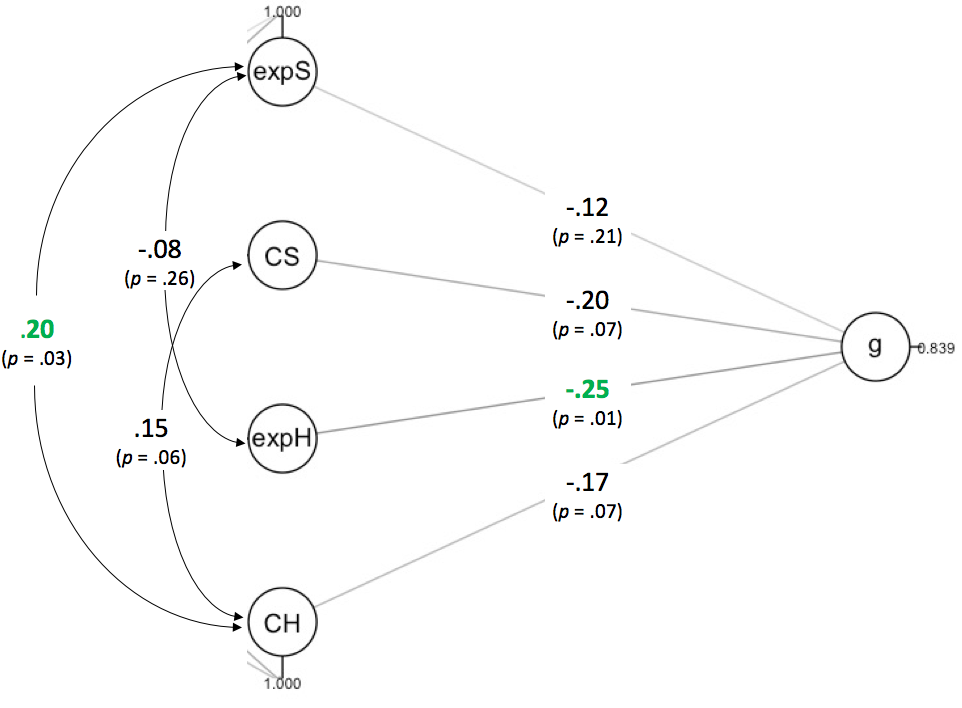
\includegraphics[width=\textwidth]{../jpg/sem1}
	\caption[CFA Platzhalter Modell 16]{Modell 16: Strukturgleichungsmodell \gls{flm} der \gls{ha}. Eingezeichnet sind die standardisierten Koeffizienten.}
	\label{fig:sem1}
\end{figure}



\section{Weitere Analysen}

%Bei der systematischen Abarbeitung der Fragestellungen haben sich weitere Fragen ergeben, welche hier ausgeführt und beantwortet werden.

\subsection{Semipartialkorrelationen}

Hier folgt noch:
\begin{itemize}
	\item Korrelationen der \gls{ss}-Bedingungen mit dem \gls{gfaktor}
	\item \ldots
\end{itemize}



% =================================================================
% D I S C U S S I O N
% =================================================================
\chapter{Diskussion \label{cha:Diskussion}}
%\ac{MLS}
\begin{itemize}
	\item Anderes Resultate, weil anderer IQ-Test eingesetzt?
	\item Anderes Resultat, weil nicht Projektor eingesetzt?
\end{itemize}

p-Wert problematisch:\\
\citet{Gelman2006}\\
\citet{Wasserstein2016}\\
\citet{Nuzzo2014}



% =================================================================
% G L O S S A R Y   &   A C R O N Y M S
% =================================================================
\printglossaries	% put this where you want your list of entries to appear 
% Important:
% 1. compile document with PdfLaTeX
% 2. run 'makeglossaries diss' in terminal
% 3. compile document with pdfLateX
% 4. -> glossaries should appear in pdf

% =================================================================
% R E F E R E N C E S 
% =================================================================
\renewcommand\bibname{Literatur}				% rename bibliography
\bibliography{bib/PhilippLibrary}				% provide .bib file
\addcontentsline{toc}{chapter}{Literatur}		% for a toc entry
%../references

% =================================================================
% A P P E N D I X   A
% =================================================================
\appendix
% not sure if this code works -----------
\setcounter{figure}{0}
\renewcommand\thefigure{\Alph{appndx}\@arabic\c@figure}
% works --------------------------
\setcounter{table}{0}
\renewcommand{\thetable}{A\arabic{table}}



\chapter{Anhang \label{cha:AAnhang}}
Dieser Anhang beschreibt die Vorgehensweise bei der Datenaufbereitung, welche zum Ausschluss von \glspl{vp} geführt hat (vgl. Abschnitt \ref{sec:Stichprobe}). Am Ende des Anhangs fasst Tabelle \ref{tab:Datenbereinigung} die Datenbereinigung zusammen.

\section{Alter}
Trotz sorgfältiger Auswahl der \glspl{vp} hat sich nachträglich bei der Altersberechnung herausgestellt, dass drei \glspl{vp} zum Testzeitpunkt noch nicht $18$~Jahre alt waren. Sie wurden vor der Analyse entfernt.


\section{\gls{ssauf}}
Zu Beginn der Datenerhebung wurde die \gls{ssauf} mit einem Kontrast von $74\,\%$ dargeboten. Nach Inspektion der ersten Daten wurde in Absprache mit Duje Tadin entschieden, den Kontrast der Aufgabe nach sieben getesteten \glspl{vp} auf $99\,\%$ zu erhöhen. Mit dieser Erhöhung des Kontrasts wurde sichergestellt, dass die über die vier Mustergrössen hinweg erwartete Verschlechterung der Wahrnehmungsleistung möglichst gross ausfällt \citep{Tadin2003}. Den restlichen \glspl{vp} wurde die Aufgabe folglich mit einem Kontrast von $99\,\%$ dargeboten und die Daten der ersten sieben \glspl{vp} der Untersuchung wurden ausgeschlossen.

Der Code, der die Darbietungszeiten generierte, hatte eine fest-codierte obere Darbietungszeitlimite von $1000$~ms. Immer wenn der adaptive Alogrithmus des QUEST-Verfahrens \citep{Watson1983} eine Darbietungszeit von $> 1000$~ms ermittelte, wurde der Stimulus deshalb der \gls{vp}  mit einer Darbietungszeit von exakt $1000$~ms präsentiert. 
Die Daten von $12$~\glspl{vp} wurden vor der Analyse entfernt, weil sie bei den sechs Schwellenschätzungen pro Mustergrösse mehr als ein Mal eine Schwellenschätzung von $> 1000$~ms erzielt haben. Exakt dasselbe Ausschlussverfahren verwendeten \citet{Melnick2013}.

Die Daten von zwei \glspl{vp} wurden von der Analyse ausgeschlossen, weil sie verglichen mit den restlichen \glspl{vp} auf der Stimulusgrösse von $1.8^{\circ}$ eine $\log_{10}$-Schwel\-len\-schätz\-ung hatten, die über das dreifache der \gls{sd} der Gesamtstichprobe betrug. Diese drei \glspl{vp} wurden nicht zur Grundpopulation gezählt und vor der Analyse entfernt. \textcolor{red}{Eventuell ausführlicher beschreiben? Darauf hinweisen, dass diese Kontrolle im log-space stattgefunden hat!!!}

%\section{\gls{ha}}
%Bei der \gls{ha} mussten keine \glspl{vp} ausgeschlossen werden.

\section{\gls{bist}}
Bei den Subtests \gls{bd}, \gls{kw}, \gls{oe}, \gls{RZ}, \gls{tg}, \gls{uw} und \gls{xg} ist der Rohwert Null im Manual des \gls{bist} keinem Punktwert zugeordnet. Vier \glspl{vp} erzielten beim Subtest \gls{xg} einen Rohwert von Null, was den Subtest nicht auswertbar machte. Die Daten dieser vier \glspl{vp} wurden vor der Analyse aufgrund dieses nicht auswertbaren Subtests entfernt. Eine \gls{vp} wurde von der Analyse ausgeschlossen, weil sie bei den \gls{b}-Subtests deutlich schlechter Abschnitt als der Rest der Stichprobe und damit einen Einfluss auf die berechneten Zusammenhänge gehabt hätte.



\begin{table}[htbp]
	\centering
	\captionsetup{labelsep = none}
	\caption[Übersicht über die Datenbereinigung]{\newline  \textit{Übersicht über die Datenbereinigung} \vspace{.2cm}}
	\label{tab:Datenbereinigung}
		\resizebox{\columnwidth}{!}{%	
	\begin{threeparttable}

			\begin{tabular}{
					l
					l
					S[table-format = 3.0]
					S[table-format = 2.0]
					S[table-format = 2.0]
					c
					S[table-format = 3.0]
					S[table-format = 2.0]
					S[table-format = 2.0]
					}
				\hline
				\multirow{2}{2cm}{Beschrieb}	& \multirow{2}{3cm}{Korrektur für}	&	\multicolumn{3}{c}{absolut}	&	&	\multicolumn{3}{c}{relativ (\%)} \\
				\cline{3-5}
				\cline{7-9}
				&&{\textit{N}} & {D} & {D kum.}	&	&	{\textit{N}} & {D} & {D kum.}\\
				\hline
				
				Getestet	&	-								&	206	&		&		&&	100	&		&		\\
							&	Alter							&	203	&	-3	&	-3	&&	89	&	-2	&	-2	\\
							&	BIS-Test						&	198	&	-5	&	-8	&&	87	&	-2	&	-4	\\
							&	Spatial-Suppression-Aufgabe		&	177	&	-21	&	-29	&&	86	&	-10	&	-14	\\
				Analysiert	&	-								&	177	&		&		&&	86	&		&		\\
				\hline
			\end{tabular}%
		%}
		\begin{tablenotes}[flushleft]
			\footnotesize				% font size
			\setlength\labelsep{0pt}	% no indent on second line
			\item \textit{Anmerkungen.} \textit{N} = Stichprobengrösse, D = Differenz, D kum. = kumulierte Differenz.
		\end{tablenotes}%
	\end{threeparttable}%
}
\end{table}


% =================================================================
% A P P E N D I X   B
% =================================================================
\chapter{Anhang \label{cha:BAnhang}}

Dieser Anhang gibt die nicht parametrischen Verfahren wieder (vgl. Abschnitt \ref{sec:Deskriptive_Statistik}).

\section{\gls{ssauf}}


Dafür wurde ein Friedman-Test durchgeführt. Der Globaltest hat gezeigt, dass die mittleren Schwellenschätzungen in den vier Bedingungen nicht identisch waren, $\upchi^2(3)=345.26$, $p<.001$. 
Um zu erfahren, welche Bedingungen sich voneinander unterschieden, wurden Post-hoc-Tests \citep{Galili2010, Hollander2014} gerechnet. Diese haben ergeben, dass sich von den (durch die vier Bedingungen bestimmten) sechs Einzelvergleichen nur die $1.8^{\circ}$- und $3.6^{\circ}$-Bedingung nicht signifikant voneinander unterschieden ($p=.09$). Die restlichen fünf Einzelvergleiche waren mit $p<.001$ alle statistisch signifikant.
Mit Ausnahme des Wahrnehmungsleistungsunterschieds zwischen der $1.8^{\circ}$- und der $3.6^{\circ}$-Bedingung verschlechterte sich die Wahrnehmungsleistung der \glspl{vp} also mit zunehmender Mustergrösse signifikant.

\section{\gls{ha}}

Um zu testen, ob die mittlere \gls{rz} der \glspl{vp} von der Anzahl Antwortalternativen abhing, wurde ein Friedman-Test durchgeführt. Der Globaltest war mit $\upchi^2(3)=516.12$, $p<.001$, hochsignifikant und belegte, dass die mittlere \gls{rz} der \glspl{vp} in den vier Bedingungen nicht identisch war. Welche Bedingungen sich voneinander unterschieden, wurde mit Post-hoc-Tests \citep{Galili2010, Hollander2014} geprüft. Diese haben gezeigt, dass sich alle Bedingungen signifikant voneinander unterschieden (alle $p\textnormal{s}<.001$). Die mittlere \gls{rz} der \glspl{vp} erhöhte sich also über die Bedingungen hinweg signifikant.

\section{\gls{bist}}

\begin{sidewaystable}
	
	
	\begin{adjustbox}{width=1\textwidth,totalheight=1\textheight,keepaspectratio}
		
		\begin{threeparttable}
			\captionsetup{labelsep = none}
			\caption[Zusammenhänge zwischen den Subtests]{\newline  \textit{Spearmans Rangkorrelationen zwischen den Subtests des \gls{bist}} \vspace{.2cm}}
			\label{tab:subtestsCorr}
			
			\sisetup{table-space-text-post = $^{*ab}$  }
			\begin{tabular}{
					c
					c
					S[table-format = 0.2, add-integer-zero=false]
					S[table-format = 0.2, add-integer-zero=false]
					S[table-format = 0.2, add-integer-zero=false]
					S[table-format = 0.2, add-integer-zero=false]
					S[table-format = 0.2, add-integer-zero=false]
					S[table-format = 0.2, add-integer-zero=false]
					S[table-format = 0.2, add-integer-zero=false]
					S[table-format = 0.2, add-integer-zero=false]
					S[table-format = 0.2, add-integer-zero=false]
					S[table-format = 0.2, add-integer-zero=false]
					S[table-format = 0.2, add-integer-zero=false]
					S[table-format = 0.2, add-integer-zero=false]
					S[table-format = 0.2, add-integer-zero=false]
					S[table-format = 0.2, add-integer-zero=false]
					S[table-format = 0.2, add-integer-zero=false]
					S[table-format = 0.2, add-integer-zero=false]
					S[table-format = 0.2, add-integer-zero=false]
					S[table-format = 0.2, add-integer-zero=false]
					>{\centering\arraybackslash}p{1.2cm}
				}
				\hline
				&	{Subtest}&	{1}	&	{2}	&	{3}	&	{4}	&	{5}	&	{6}	&	{7}	&	{8}	&	{9}	&	{10}&	{11}&	{12}&	{13}&	{14}&	{15}&	{16}&	{17}&	{18}	\\
				\hline
				
1	&	OG	&					&	.02				&	.05			&.00	&.04	&-.05	&.01	&-.12	&-.02	&.04	&.03	&-.01	&-.02	&.00	&.01	&-.02	&.04	&-.03	\\
2	&	ZN	&	.25{$^{***}$}	&					&	.00			&.01	&.00	&.02	&.00	&.00	&.01	&.04	&.02	&-.03	&.01	&.01	&.00	&.03	&.06	&.04	\\
3	&	AN	&	.26{$^{***}$}	&	.42{$^{***}$}	&				&-.03	&.02	&-.02	&.03	&-.12	&-.01	&.01	&.01	&-.03	&-.01	&.05	&.00	&.01	&.05	&.02	\\
4	&	XG	&	.21{$^{**}$}	&	.55{$^{***}$}	&	.35{$^{***}$}	&	&.01	&.01	&-.04	&-.08	&.00	&.01	&.02	&-.05	&.00	&.00	&-.03	&.01	&.01	&.03	\\
5	&	WA	&	.31{$^{***}$}	&	.41{$^{***}$}	&	.47{$^{***}$}	&	.34{$^{***}$}	&&-.01	&.03	&-.03	&.01	&.01	&.01	&-.02	&-.01	&.06	&.01	&.01	&.05&.00\\
6	&	ZP	&	.27{$^{***}$}	&	.15{$^a$}		&	.15{$^{*}$}	&	.30{$^{***}$}	&	.17{$^{*}$}		&	&	-.03&-.04	&.00	&.02	&-.01	&-.03	&-.02	&.01	&.00	&.03	&-.02	&.02	\\
7	&	TM	&	.29{$^{***}$}	&	.26{$^{***}$}	&	.41{$^{***}$}	&	.36{$^{***}$}	&	.48{$^{***}$}	&	.24{$^{**}$}	&	&-.07	&.00	&.02	&.02	&-.04	&-.03	&.05	&.02	&.01	&.01	&.02	\\
8	&	BD	&	.19{$^{*}$}		&	.08				&	.17{$^{*}$}		&	.19{$^{*}$}		&	.02				&	.08				&	.10	&	&-.05	&.02	&-.05	&-.07	&-.05	&-.05	&-.04	&-.02	&-.12	&-.06	\\
9	&	SC	&	.16{$^{*}$}		&	.51{$^{***}$}	&	.35{$^{***}$}	&	.48{$^{***}$}	&	.22{$^{**}$}	&	.17{$^{*}$}		&	.32{$^{***}$}	&	.25{$^{***}$}	&	&.01	&.01	&.01&.00&-.03	&.02&.01	&.01&.01\\
10	&	ST	&	.34{$^{***}$}	&	.15	{$^{*}$}	&	.23{$^{**}$}	&	.30{$^{***}$}	&	.31{$^{***}$}	&	.22{$^{**}$}	&	.37{$^{***}$}	&	-.03			&	.22{$^{**}$}	&		&.04&.02&.00&-.05&.03&.02&.04&.03\\
11	&	CH	&	.33{$^{***}$}	&	.49{$^{***}$}	&	.51{$^{***}$}	&	.29{$^{***}$}	&	.50{$^{***}$}	&	.14				&	.30				&	.12				&	.31{$^{***}$}	&	.13	&	&-.01&.01&.01&.00&.02&.07&.02	\\
12	&	TG	&	.33{$^{***}$}	&	.36{$^{***}$}	&	.30{$^{***}$}	&	.48{$^{***}$}	&	.45{$^{***}$}	&	.19{$^{*}$}		&	.47{$^{***}$}	&	.18{$^{*}$}		&	.26{$^{***}$}&	.36{$^{***}$}	&	.23{$^{**}$}	&	&-.08&.00&-.05&.02&.00&.00	\\
13	&	RZ	&	.32{$^{***}$}	&	.52{$^{***}$}	&	.42{$^{***}$}	&	.55{$^{***}$}	&	.44{$^{***}$}	&	.29{$^{***}$}	&	.45{$^{***}$}	&	.13				&	.44{$^{***}$}&	.34{$^{***}$}	&	.37{$^{***}$}	&	.41{$^{***}$}&&-.03&.01&.01&.02&.01	\\
14	&	WM	&	.41{$^{***}$}	&	.10				&	.24{$^{**}$}	&	.18{$^{*}$}		&	.20{$^{**}$}	&	.26{$^{***}$}	&	.34{$^{***}$}	&	.13				&	.13			&	.45{$^{***}$}	&	.16{$^{*}$}		&	.18{$^{*}$}		&	.15{$^{*}$}	&&-.01&.01&-.02&-.03	\\
15	&	KW	&	.26{$^{***}$}	&	.24{$^{***}$}	&	.28{$^{***}$}	&	.39{$^{***}$}	&	.39{$^{***}$}	&	.24{$^{**}$}	&	.54{$^{***}$}	&	.19{$^{*}$}		&	.26{$^{***}$}&	.49{$^{***}$}	&	.21{$^{**}$}	&	.60{$^{***}$}	&	.35{$^{***}$}	&	.34{$^{***}$}	&&.03&.04&-.01	\\
16	&	ZZ	&	.31{$^{***}$}	&	.02				&	.03				&	.20{$^{**}$}	&	.00				&	.34{$^{***}$}	&	.09				&	.11				&	.04			&	.28{$^{***}$}	&	.05				&	.05				&	.08				&	.38{$^{***}$}	&	.10	&&.02&.01	\\
17	&	OE	&	.06				&	-.01			&	-.01			&	.07				&	-.05			&	.04				&	.12				&	.46{$^{***}$}	&	.15{$^{*}$}&	-.01			&	-.13			&	.15{$^{*}$}		&	.13					&	.03	&	.13		& -.05&&.02	\\
18	&	WE	&	.42{$^{***}$}	&	.27{$^{***}$}	&	.26{$^{***}$}	&	.19{$^{*}$}		&	.29{$^{***}$}	&	.25{$^{***}$}	&	.06				&	.04				&	.14			&	.21{$^{**}$}	&	.25{$^{**}$}	&	.20{$^{**}$}	&	.33{$^{***}$}	&.19{$^{*}$}&	.23{$^{**}$}&.18{$^{*}$}&-.12&\\
\hline			
			\end{tabular}
			
			\begin{tablenotes}[flushleft]
				\footnotesize				% font size
				\setlength\labelsep{0pt}	% no indent on second line
				\item \textit{Anmerkung.} Siehe Tabelle \ref{tab:BIS} für eine Beschreibung der Subtests.
				\item {$^a$}Der exakte Zusammenhang betrug $r_{s}=.147$, $p=.051$. Alle restlichen in der Tabelle mit $r_{s}=.15$ bezeichneten Korrelationskoeffizienten wiesen \textit{p}-Werte $<.05$ auf.
				\item {$^{*}$}$p<.05$. {$^{**}$}$p<.01$. {$^{***}$}$p<.001$ (zweiseitig).
			\end{tablenotes}
			
		\end{threeparttable}
	\end{adjustbox}
	
\end{sidewaystable}

\section{Zusammenhangsmasse}

Bevor ausgewählte Zusammenhänge zwischen den Aufgaben in den folgenden Abschnitten mit den Fragestellungen abgearbeitet werden, ist der Vollständigkeit halber in Tabelle \ref{tab:rank_order_correlations_manifest} eine umfassende Korrelationsmatrix abgebildet. 

Abgesehen von den bereits erwähnten Zusammenhängen innerhalb der Bedingungen der \gls{ssauf} respektive der \gls{ha} und den noch zu besprechenden Zusammenhängen ist an dieser Stelle gesondert auf Folgendes hinzuweisen.
Der \gls{si} wies eine negative Korrelation mit der $1.8^{\circ}$-Be\-ding\-ung auf ($r_{s}=-.33$, $p<.001$) und korrelierte positiv mit der $7.2^{\circ}$-Bedingung ($r_{s}=.53$, $p<.001$). 
Diese Zusammenhänge können als Hinweis dafür gesehen werden, dass der \gls{si} als Differenz zwischen der $\log_{10}$-Schwel\-len\-schätz\-ung für die Mustergrösse $7.2^{\circ}$ und der $\log_{10}$-Schwel\-len\-schätz\-ung für die Mustergrösse $1.8^{\circ}$ korrekt gebildet wurde.
Weiter korrelierte einzig die 0-bit-Bedingung der \gls{ha} signifikant mit der $3.6^{\circ}$- und der $5.4^{\circ}$-Bedingung der \gls{ssauf}  ($r_{s}=.19$ respektive $r_{s}=.16$, beide $p\textnormal{s}<.05$), während alle restlichen Zusammenhänge zwischen den beiden Aufgaben so gering ausfielen, dass sie die gewählte Irrtumswahrscheinlichkeit von weniger als $5\,\%$ nicht erreichten.
Und als letztes sei noch erwähnt, dass die Bedingungen der \gls{ha} alle erwartungsgemäss  signifikant negativ mit dem \gls{zwert} des \gls{bist} korrelierten \citep[$r_{s}=-.15$ bis $-.32$, alle $p\textnormal{s}<.05$; vgl. ][]{Sheppard2008}, während die Bedingungen der \gls{ssauf} hingegen alle nicht signifikant mit dem \gls{zwert} zusammenhingen ($r_{s}=.04$ bis $-.14$, alle $p\textnormal{s}>.05$).


\begin{sidewaystable}
	
	\begin{adjustbox}{width=.80\textwidth, keepaspectratio}
		
		\begin{threeparttable}
			\centering
			\captionsetup{labelsep = none}
			\caption[Korrelationen zwischen den Aufgaben]{\newline  \textit{Spearmans Rangkorrelationen zwischen den Bedingungen der \gls{ssauf}, dem \gls{si}, den Bedingungen der \gls{ha}, dem \textit{z}-Wert und dem \gls{gfaktor} des \gls{bist}} \vspace{.2cm}}
			\label{tab:rank_order_correlations_manifest}
			\sisetup{table-space-text-post = $^{***}$}
			\begin{tabular}{
					c
					c
					S[table-format = 0.2, add-integer-zero=false]
					S[table-format = 0.2, add-integer-zero=false]
					S[table-format = 0.2, add-integer-zero=false]
					S[table-format = 0.2, add-integer-zero=false]
					S[table-format = 0.2, add-integer-zero=false]
					p{.001cm}
					S[table-format = 0.2, add-integer-zero=false]
					S[table-format = 0.2, add-integer-zero=false]
					S[table-format = 0.2, add-integer-zero=false]
					S[table-format = 0.2, add-integer-zero=false]
					p{.001cm}
					S[table-format = 0.2, add-integer-zero=false]
					S[table-format = 0.2, add-integer-zero=false]
					>{\centering\arraybackslash}p{1.2cm}
				}
				\hline
				
				
				&	& 	\multicolumn{5}{c}{\gls{ssauf}}	&	&	\multicolumn{4}{c}{\gls{ha}}	&	&	\multicolumn{2}{c}{\gls{bist}}	\\
				
				\cline{3-7}
				\cline{9-12}
				\cline{14-15}
				
				&	{Mass}			&	{1}				&	{2}				&	{3}				&	 {4}	& {5}& 	& {6}	& {7}	& {8}	&{9}&&{10}&{11} \\
				\hline
				1	&	$1.8^{\circ}$	&		&		&		&		&		&		&		&		&		&		&\\
				2	&	$3.6^{\circ}$	&	.84{$^{***}$}	&		&		&		&		&		&		&		&		&		&\\
				3	&	$5.4^{\circ}$	&	.73{$^{***}$}	&	.86{$^{***}$}	&		&		&		&		&		&		&		&		&\\
				4	&	$7.2^{\circ}$	&	.55{$^{***}$}	&	.76{$^{***}$}	&	.88{$^{***}$}	&		&		&		&		&		&		&		&\\
				5	&	SI 				&	-.33{$^{***}$}	&	.03				&	.26{$^{***}$}	&	.53{$^{***}$}	& & & & & & & \\
				\rule{0pt}{4ex}%  EXTRA vertical height
				6	&	0-bit			&	.12				&	.19{$^{**}$}	&	.16{$^{*}$}	&	.12		&.01&	&		&&&&&\\
				7	&	1-bit			&	.03				&	.06				&	.03			&	.00		&-.05&	&.72{$^{***}$}	&	&	&	&	&		\\
				8	&	2-bit			&	.11				&	.11				&	.07			&	.04		&-.08&	&.52{$^{***}$}	&	.71{$^{***}$}	&	&	&	&		\\
				9	&	2.58-bit		&	.07				&	.05				&	.02			&	-.01	&-.09&	&.40{$^{***}$}	&	.63{$^{***}$}	&	.81{$^{***}$}	&	&	&		\\
				\rule{0pt}{4ex}%  EXTRA vertical height
				10	&	\textit{z}-Wert	&	-.14			&	-.12			&	-.09		&	-.06	&.04&	&	-.15{$^{*}$}	&	-.32{$^{***}$}	&	-.31{$^{***}$}	&	-.31{$^{***}$}	&				&		\\
				11	&	\gls{gfaktor}	&	-.18{$^{*}$}	&	-.18{$^{*}$}	&	-.14		&	-.11	&.03&	&	-.15{$^{*}$}	&	-.29{$^{***}$}	&	-.29{$^{***}$}	&	-.28{$^{***}$}	&				&	.97{$^{***}$}	\\
				\hline
				
			\end{tabular}%
			%}
			\begin{tablenotes}[flushleft]
				\footnotesize				% font size
				\setlength\labelsep{0pt}	% no indent on second line
				\item \textit{Anmerkungen}. SI = \gls{si}. \gls{zwert} = Mittelwert aus allen 18 \textit{z}-standardisierten Subtests.
				\item {$^{*}$}$p<.05$. {$^{**}$}$p<.01$. {$^{***}$}$p<.001$ (zweiseitig).
			\end{tablenotes}
			
		\end{threeparttable}%
	\end{adjustbox}
	
\end{sidewaystable}

\end{document}




